% UCL Thesis LaTeX Template
%  See below for info

%%%%%%%%%%%%% Preamble/Setup %%%%%%%%%%%%%%%%%
% This package goes first
\RequirePackage[l2tabu, orthodox]{nag}


% ------ Main document class specification ------
% The draft option here prevents images being inserted,
% Option = phd : )
%\documentclass[12pt,phd,draft,a4paper,oneside]{ucl_thesis}
\documentclass[11pt,phd,a4paper,oneside]{ucl_thesis}
\usepackage{mathptmx}
\usepackage[11pt]{moresize}
\setlength \parskip {1em}

% Package configuration:
% -------- Packages --------

% This package just gives you a quick way to dump in some sample text.
% You can remove it -- it's just here for the examples.
\usepackage{blindtext}

% This package means empty pages (pages with no text) won't get stuff
%  like chapter names at the top of the page. It's mostly cosmetic.
\usepackage{emptypage}

% The graphicx package adds the \includegraphics command,
%  which is your basic command for adding a picture.
\usepackage{graphicx}

% This command is provided by the graphicx package, and 
%  controls the default dpi resolution of images you use.
%  72 is the default, but 300 is more normal, and 600 is
%  as good as you can expect to be able to get on normal paper.
%\pdfimageresolution=300


% The float package improves LaTeX's handling of floats,
%  and also adds the option to *force* LaTeX to put the float
%  HERE, with the [H] option to the float environment.
\usepackage{float}

\usepackage{placeins}

% The amsmath package enhances the various ways of including
%  maths, including adding the align environment for aligned
%  equations.
\usepackage{amsmath}

% Use these two packages together -- they define symbols
%  for e.g. units that you can use in both text and math mode.
\usepackage{gensymb}
\usepackage{textcomp}
% You may also want the units package for making little
%  fractions for unit specifications.
%\usepackage{units}


% The setspace package lets you use 1.5-sized or double line spacing.
\usepackage{setspace}
\setstretch{1.5}

% That just does body text -- if you want to expand *everything*,
%  including footnotes and tables, use this instead:
%\renewcommand{\baselinestretch}{1.5}


% PGFPlots is either a really clunky or really good way to add graphs
%  into your document, depending on your point of view.
% There's waaaaay too much information on using this to cover here,
%  so, you might want to start here:
%   http://pgfplots.sourceforge.net/
%  or here:
%   http://pgfplots.sourceforge.net/pgfplots.pdf
%\usepackage{pgfplots}
%\pgfplotsset{compat=1.3} % <- this fixed axis labels in the version I was using

% PGFPlotsTable can help you make tables a little more easily than
%  usual in LaTeX.
% If you're going to have to paste data in a lot, I'd suggest using it.
%  You might want to start with the manual, here:
%  http://pgfplots.sourceforge.net/pgfplotstable.pdf
%\usepackage{pgfplotstable}

% These settings are also recommended for using with pgfplotstable.
%\pgfplotstableset{
%	% these columns/<colname>/.style={<options>} things define a style
%	% which applies to <colname> only.
%	empty cells with={--}, % replace empty cells with '--'
%	every head row/.style={before row=\toprule,after row=\midrule},
%	every last row/.style={after row=\bottomrule}
%}


% The mhchem package provides chemistry formula typesetting commands
%  e.g. \ce{H2O}
%\usepackage[version=3]{mhchem}

% And the chemfig package gives a weird command for adding Lewis 
%  diagrams, for e.g. organic molecules
%\usepackage{chemfig}

% The linenumbers command from the lineno package adds line numbers
%  alongside your text that can be useful for discussing edits 
%  in drafts.
% Remove or comment out the command for proper versions.
%\usepackage[modulo]{lineno}
% \linenumbers 


% Alternatively, you can use the ifdraft package to let you add
%  commands that will only be used in draft versions
%\usepackage{ifdraft}

% For example, the following adds a watermark if the draft mode is on.
%\ifdraft{
%  \usepackage{draftwatermark}
%  \SetWatermarkText{\shortstack{\textsc{Draft Mode}\\ \strut \\ \strut \\ \strut}}
%  \SetWatermarkScale{0.5}
%  \SetWatermarkAngle{90}
%}


% The multirow package adds the option to make cells span 
%  rows in tables.
\usepackage{multirow}

%%\usepackage{fourier} 
\usepackage{array}
\usepackage{makecell}

\renewcommand\theadalign{bc}
\renewcommand\theadfont{\bfseries}
\renewcommand\theadgape{\Gape[4pt]}
\renewcommand\cellgape{\Gape[4pt]}


% Subfig allows you to create figures within figures, to, for example,
%  make a single figure with 4 individually labeled and referenceable
%  sub-figures.
% It's quite fiddly to use, so check the documentation.
%\usepackage{subfig}

% The natbib package allows book-type citations commonly used in
%  longer works, and less commonly in science articles (IME).
% e.g. (Saucer et al., 1993) rather than [1]
% More details are here: http://merkel.zoneo.net/Latex/natbib.php
%\usepackage{natbib}
\usepackage{url}

% The bibentry package (along with the \nobibliography* command)
%  allows putting full reference lines inline.
%  See: 
%   http://tex.stackexchange.com/questions/2905/how-can-i-list-references-from-bibtex-file-in-line-with-commentary
\usepackage{bibentry} 

% The isorot package allows you to put things sideways 
%  (or indeed, at any angle) on a page.
% This can be useful for wide graphs or other figures.
%\usepackage{isorot}

% The caption package adds more options for caption formatting.
% This set-up makes hanging labels, makes the caption text smaller
%  than the body text, and makes the label bold.
% Highly recommended.
\usepackage[format=hang,font=small,labelfont=bf]{caption}
\usepackage{subcaption}

% If you're getting into defining your own commands, you might want
%  to check out the etoolbox package -- it defines a few commands
%  that can make it easier to make commands robust.
\usepackage{etoolbox}

% For lists
\usepackage{enumitem}
\setlist{nosep}

\usepackage{siunitx}

\DeclareSIUnit\mm{\milli\metre}
\DeclareSIUnit\km{\kilo\metre}


\DeclareSIUnit\micron{\micro\metre}
\DeclareSIUnit\mrad{\milli\rad}
\DeclareSIUnit\gauss{G}
\DeclareSIUnit\eVperc{\eV\per\clight}

\DeclareSIUnit\TeV{\teva\ev}
\DeclareSIUnit\GeV{\giga\ev}
\DeclareSIUnit\MeV{\mega\ev}

\DeclareSIUnit\nanobarn{\nano\barn}
\DeclareSIUnit\picobarn{\pico\barn}
\DeclareSIUnit\femtobarn{\femto\barn}
\DeclareSIUnit\attobarn{\atto\barn}
\DeclareSIUnit\zeptobarn{\zepto\barn}
\DeclareSIUnit\yoctobarn{\yocto\barn}

\DeclareSIUnit\nb{\nano\barn}
\DeclareSIUnit\pb{\pico\barn}
\DeclareSIUnit\fb{\femto\barn}
\DeclareSIUnit\ab{\atto\barn}
\DeclareSIUnit\zb{\zepto\barn}
\DeclareSIUnit\yb{\yocto\barn}

%%%%%% From ATLAS stuff
% +--------------------------------------------------------------------+
% |                                                                    |
% |  Useful things for proton-proton physics                           |
% |                                                                    |
% +--------------------------------------------------------------------+
%
\def\mjj{\ensuremath{m_{jj}}}
\def\pt{\ensuremath{p_{\mathrm{T}}}} % Subscript roman not italic (EE)
\def\pT{\ensuremath{p_{\mathrm{T}}}} % Subscript roman not italic (EE)
\def\et{\ensuremath{E_{\mathrm{T}}}} % Subscript roman not italic (EE)
\def\eT{\ensuremath{E_{\mathrm{T}}}} % Subscript roman not italic (EE)
\def\ET{\ensuremath{E_{\mathrm{T}}}} % Subscript roman not italic (EE)
\def\HT{\ensuremath{H_{\mathrm{T}}}} % Subscript roman not italic (EE)
\def\ptsq{\ensuremath{p^2_{\mathrm{T}}}} % Fixed so it works correctly (EE)

\def\degr{\ensuremath{^\circ}} % Removed mbox - caused problems and not needed (EE)
\def\abseta{\ensuremath{|\eta|}}
\def\Hgg{\ensuremath{H\to\gamma\gamma}}
\def\mh{\ensuremath{m_h}}
\def\mW{\ensuremath{m_W}}
\def\mZ{\ensuremath{m_Z}}
\def\mH{\ensuremath{m_H}}
\def\mA{\ensuremath{m_A}}
\def\MET{\ensuremath{E_{\mathrm{T}}^{\mathrm{miss}}}} % Sub/superscript roman not italic (EE)
\def\met{\ensuremath{E_{\mathrm{T}}^{\mathrm{miss}}}} % Sub/superscript roman not italic (EE)
\def\Wjj{\ensuremath{W \rightarrow jj}}
\def\tjjb{\ensuremath{t \rightarrow jjb}}
\def\Hbb{\ensuremath{H \rightarrow b\bar b}}
\def\Zmm{\ensuremath{Z \rightarrow \mu\mu}}
\def\Zee{\ensuremath{Z \rightarrow ee}}
\def\Zll{\ensuremath{Z \rightarrow \ell\ell}}
\def\Wln{\ensuremath{W \rightarrow \ell\nu}}
\def\Wen{\ensuremath{W \rightarrow e\nu}}
\def\Wmn{\ensuremath{W \rightarrow \mu\nu}}
\def\Hllll{\ensuremath{H \rightarrow ZZ^{(*)} \rightarrow \mu\mu\mu\mu}}
\def\Hmmmm{\ensuremath{H \rightarrow \mu\mu\mu\mu}}
\def\Heeee{\ensuremath{H \rightarrow eeee}}
\def\Amm{\ensuremath{A \rightarrow \mu\mu}}
\def\Ztau{\ensuremath{Z \rightarrow \tau\tau}}
\def\Wtau{\ensuremath{W \rightarrow \tau\nu}}
\def\Atau{\ensuremath{A \rightarrow \tau\tau}}
\def\Htau{\ensuremath{H \rightarrow \tau\tau}}
\def\begL{10$^{31}$~cm$^{-2}$~s$^{-1}$}
\def\lowL{10$^{33}$~cm$^{-2}$~s$^{-1}$}
\def\highL{10$^{34}$~cm$^{-2}$~s$^{-1}$}
\newcommand{\EjetRec}{\ensuremath{E_{\mathrm{rec}}}} % Subscript roman not italic (EE)
\newcommand{\PjetRec}{\ensuremath{p_{\mathrm{rec}}}} % Subscript roman not italic (EE)
\newcommand{\EjetTru}{\ensuremath{E_{\mathrm{truth}}}} % Subscript roman not italic (EE)
\newcommand{\PjetTru}{\ensuremath{p_{\mathrm{truth}}}} % Subscript roman not italic (EE)
\newcommand{\EjetDM}{\ensuremath{E_{\mathrm{DM}}}} % Subscript roman not italic (EE)
\newcommand{\Rcone}{\ensuremath{R_{\mathrm{cone}}}} % Subscript roman not italic (EE)
%
% +--------------------------------------------------------------------+
% |                                                                    |
% |  Some useful units                                                 |
% |                                                                    |
% +--------------------------------------------------------------------+
%
\def\TeV{\ifmmode {\mathrm{\ Te\kern -0.1em V}}\else
                   \textrm{Te\kern -0.1em V}\fi}%
\def\GeV{\ifmmode {\mathrm{\ Ge\kern -0.1em V}}\else
                   \textrm{Ge\kern -0.1em V}\fi}%
\def\MeV{\ifmmode {\mathrm{\ Me\kern -0.1em V}}\else
                   \textrm{Me\kern -0.1em V}\fi}%
\def\keV{\ifmmode {\mathrm{\ ke\kern -0.1em V}}\else
                   \textrm{ke\kern -0.1em V}\fi}%
\def\eV{\ifmmode  {\mathrm{\ e\kern -0.1em V}}\else
                   \textrm{e\kern -0.1em V}\fi}%
\let\tev=\TeV
\let\gev=\GeV
\let\mev=\MeV
\let\kev=\keV
\let\ev=\eV

\def\TeVc{\ifmmode {\mathrm{\ Te\kern -0.1em V}/c}\else
                   {\textrm{Te\kern -0.1em V}/$c$}\fi}%
\def\GeVc{\ifmmode {\mathrm{\ Ge\kern -0.1em V}/c}\else
                   {\textrm{Ge\kern -0.1em V}/$c$}\fi}%
\def\MeVc{\ifmmode {\mathrm{\ Me\kern -0.1em V}/c}\else
                   {\textrm{Me\kern -0.1em V}/$c$}\fi}%
\def\keVc{\ifmmode {\mathrm{\ ke\kern -0.1em V}/c}\else
                   {\textrm{ke\kern -0.1em V}/$c$}\fi}%
\def\eVc{\ifmmode  {\mathrm{\ e\kern -0.1em V}/c}\else
                   {\textrm{e\kern -0.1em V}/$c$}\fi}%
\let\tevc=\TeVc
\let\gevc=\GeVc
\let\mevc=\MeVc
\let\kevc=\keVc
\let\evc=\eVc

\def\TeVcc{\ifmmode {\mathrm{\ Te\kern -0.1em V}/c^2}\else
                   {\textrm{Te\kern -0.1em V}/$c^2$}\fi}%
\def\GeVcc{\ifmmode {\mathrm{\ Ge\kern -0.1em V}/c^2}\else
                   {\textrm{Ge\kern -0.1em V}/$c^2$}\fi}%
\def\MeVcc{\ifmmode {\mathrm{\ Me\kern -0.1em V}/c^2}\else
                   {\textrm{Me\kern -0.1em V}/$c^2$}\fi}%
\def\keVcc{\ifmmode {\mathrm{\ ke\kern -0.1em V}/c^2}\else
                   {\textrm{ke\kern -0.1em V}/$c^2$}\fi}%
\def\eVcc{\ifmmode  {\mathrm{\ e\kern -0.1em V}/c^2}\else
                   {\textrm{e\kern -0.1em V}/$c^2$}\fi}%
\let\tevcc=\TeVcc
\let\gevcc=\GeVcc
\let\mevcc=\MeVcc
\let\kevcc=\keVcc
\let\evcc=\eVcc

\def\cm{\ifmmode  {\mathrm{\ cm}}\else
                   \textrm{~cm}\fi}%
%
\def\ifb{\mbox{fb$^{-1}$}}%  Inverse femtobarns.
\def\ipb{\mbox{pb$^{-1}$}}%  Inverse picobarns.
\def\inb{\mbox{nb$^{-1}$}}%  Inverse nanobarns.
%
\def\mass#1{\ensuremath{m_{#1#1}}}%  "\mass{\mu}" produces "msub{mumu}".
\def\twomass#1#2{\ensuremath{m_{#1#2}}}% 
%
\def\Ecm{\ensuremath{E_{\mathrm{cm}}}} % Subscript roman not italic (EE)
%

\def\gt{\ensuremath{>}}
\def\lt{\ensuremath{<}}

\def\Like{\ensuremath{\mathcal{L}}}

% Sets up links within your document
%%
%% This file uses the hyperref package to make your thesis have metadata embedded in the PDF, 
%%  and also adds links to be able to click on references and contents page entries to go to 
%%  the pages.
%%

% Some hacks are necessary to make bibentry and hyperref play nicely.
% See: http://tex.stackexchange.com/questions/65348/clash-between-bibentry-and-hyperref-with-bibstyle-elsart-harv
\usepackage{bibentry}
\makeatletter\let\saved@bibitem\@bibitem\makeatother
\usepackage[pdftex,hidelinks]{hyperref}
\makeatletter\let\@bibitem\saved@bibitem\makeatother
\makeatletter
\AtBeginDocument{
    \hypersetup{
        pdfsubject={Thesis Subject},
        pdfkeywords={Thesis Keywords},
        pdfauthor={Author},
        pdftitle={Title},
    }
}
\makeatother
    

% And then some settings in separate files.
% These settings are from:
%  http://mintaka.sdsu.edu/GF/bibliog/latex/floats.html

% They give LaTeX more options on where to put your figures, and may
%  mean that fewer of your figures end up at the tops of pages far
%  away from the thing they're related to.

% Alters some LaTeX defaults for better treatment of figures:
% See p.105 of "TeX Unbound" for suggested values.
% See pp. 199-200 of Lamport's "LaTeX" book for details.

%   General parameters, for ALL pages:
\renewcommand{\topfraction}{0.9}	% max fraction of floats at top
\renewcommand{\bottomfraction}{0.8}	% max fraction of floats at bottom

%   Parameters for TEXT pages (not float pages):
\setcounter{topnumber}{2}
\setcounter{bottomnumber}{2}
\setcounter{totalnumber}{4}     % 2 may work better
\setcounter{dbltopnumber}{2}    % for 2-column pages
\renewcommand{\dbltopfraction}{0.9}	% fit big float above 2-col. text
\renewcommand{\textfraction}{0.07}	% allow minimal text w. figs

%   Parameters for FLOAT pages (not text pages):
\renewcommand{\floatpagefraction}{0.7}	% require fuller float pages
% N.B.: floatpagefraction MUST be less than topfraction !!
\renewcommand{\dblfloatpagefraction}{0.7}	% require fuller float pages

%Adjust space around figures
\setlength{\textfloatsep}{20pt plus 4.0pt minus 2.0pt}
\setlength{\intextsep}   {20pt plus 4.0pt minus 2.0pt}
% remember to use [htp] or [htpb] for placement,
% e.g. 
%  \begin{figure}[htp]
%   ...
%  \end{figure}
\usepackage[bottom]{footmisc}
 % For things like figures and tables
\bibliographystyle{unsrt}   % For bibliographies
%%%%%%%%%%%%%%%%%%%%%%%%%%%%%%%%%%%


%%%%%%%%%%%%% Content starts here %%%%%%%%%%%%%%%%%
% Title Settings
\setcounter{secnumdepth}{3}
\setcounter{tocdepth}{3}
%\title{ \Huge In the Search of Beauty:\\ \vspace{0.3em} Searches for New Physics using \mbox{Pairs of Jets Containing $b$-quarks} \mbox{at the ATLAS Detector}}
\title{\Huge  Searches for New Physics using \mbox{Pairs of Jets Containing $b$-quarks} \mbox{at the ATLAS Detector}}
\author{\LARGE Laurie M\hspace{1pt}$\textsuperscript{c}$\hspace{-1pt}Clymont}
\department{Department of Physics and Astronomy,}

\begin{document}

\nobibliography*
% Lets you put bibliography entries whereever you like.
 

% If you haven't finished making your full BibTex file yet, you
%  might find this useful -- it'll just replace all your
%  citations with little superscript notes.
% Uncomment to use.
%\renewcommand{\cite}[1]{\emph{\textsuperscript{[#1]}}}

% At last, content! Remember filenames are case-sensitive and 
%  *must not* include spaces.
\maketitle
\makedeclaration

\begin{abstract} % 300 word limit

Two searches for Beyond Standard Model resonances are performed                                                                                 %% 9
%decaying to a pair of $b$-quarks or a $b$-quark and a gluon are performed.                                                                     %%%%%
using 13~TeV \mbox{proton--proton} collision data collected by the ATLAS detector in 2015 and 2016                                              %% 16
using the invariant mass distribution of pairs of jets,                                                                                         %% 9
where at least one or both jets are identified as containing a \mbox{$b$-quark}.                                                                %% 13
The searches are sensitive to resonances decaying to a pair of \mbox{$b$-quarks} or a \mbox{$b$-quark} and a gluon.                             %% 18
A high-mass search probes the mass region 1.4~--~6~TeV using a data-set corresponding to an integrated luminosity of 13.3~\ifb{}.               %% 22
A low-mass search utilises real-time $b$-jet identification to                                                                                  %% 10
probe the mass region 0.6~--~1.5~TeV using a data-set corresponding to an integrated luminosity of 24.3~\ifb{}.                                 %% 18
No evidence of a resonance is found.                                                                                                            %% 7
Excited $b^*$ quarks with masses from 1.4 to 2.3~TeV and                                                                                        %% 11                        
a set of $Z'$ boson models with masses from 0.6 to 1.25~TeV or at 1.5~TeV are excluded at the 95\% credibility-level.                           %% 24
In addition, 95\% credibility-level upper limits are set on generic signals with a Gaussian distribution in the mass range 0.65~--~6~TeV.               %% 20

\end{abstract}                                                                                                                                  %% == 177

\begin{acknowledgements}

%% Andreas
I would like to thank Andreas for always being eager to provide advice, support and macchiatos.
Your supervision has made this thesis possible and is greatly appreciated.

%% Di-b-jet
Thanks to Rui, Andrea, Bing, Nishu, Sergei, Jeff, Jimmy and all those I worked with in the di-$b$-jet analysis team;
I hope that your hard work is given justice in this thesis.

%% ATLAS postdocs
I would also like to thank all the students, fellows and post-docs at ATLAS and UCL who provided help throughout my PhD;
the way that so many are always willing to drop what they are doing to aid another is something that makes ATLAS a great collaboration to be a part of.
Particular thanks go to Tim, Kate, John and Gabriel for always providing help and guidance when I needed it.
Also thanks to Andy and Jiggins for putting up with me in the office for so long and answering every one of my inane questions.

%% Family
Thanks to my family and friends in Manchester, Glasgow, London and Geneva who have made the last three and a bit years an enjoyable experience.

%% Parents
Finally, a huge thanks to my parents who have always supported and encouraged me;
without you this wouldn't have been possible. 

\end{acknowledgements}

\setcounter{tocdepth}{2} 
% Setting this higher means you get contents entries for
%  more minor section headers.

\tableofcontents
\listoffigures
\listoftables


\chapter{Introduction}
\label{sec:int}
%\vspace{-2em}
The Standard Model is the current best description of the fundamental particles of the universe and their interactions.
However, inconsistencies within the Standard Model indicate that
there must be Beyond Standard Model (BSM) physics.
Many proposed BSM models predict the existence of new particles
which preferentially decay to a pair of $b$-quarks or a $b$-quark and a gluon.
The observation of such a BSM particle would provide crucial experimental
evidence in the development of a more complete theory of particle physics.

%The high-energy $pp$ collisions produced by the LHC and observed
%by the ATLAS experiment provide an opportunity to search for
%BSM phyics in unexplored regions of phase space.

One experimental technique to discover a BSM particle is to search for
the dominant resonant production of that particle using a particle collider.
Resonant production occurs when the invariant mass of the colliding partons is equal to the mass of the BSM particle.
The experimental signature of resonant production is known as a resonance.

Many searches for resonances of BSM particles decaying to a pair of quarks or gluons
have been performed using the invariant mass distribution of pairs of hadronic jets created
by high-energy hadron collisions~\cite{theo-dijet_harris}, such searches are known as inclusive dijet searches.
%Dijet searches are particularly interesting at hadron colliders as BSM particles
%that decay to quarks will be strongly produced.
Inclusive dijet searches have been performed using 13~TeV \mbox{proton--proton} ($pp$) collisions at the
Large Hadron Collider (LHC) by the ATLAS and CMS collaborations;
the searches have probed the mass ranges 1.1~--~8~TeV~\cite{dijet-mori16_paper,dijet-mori17_paper,dijet-cms}
and 0.1~--~1.5~TeV~\cite{dijet-isr,dijet-TLA,dijet-isr_cms},
no evidence of a BSM resonance has yet been found.

The sensitivity of dijet searches to BSM particles decaying to one or two $b$-quarks can be increased
using $b$-jets, where a $b$-jet is a hadronic jet containing a $b$-quark.
Such searches are known as di-$b$-jet searches.
Di-$b$-jet searches have previously been performed by
the CDF collaboration using 1.8~TeV $p\bar{p}$ collisions at the Tevatron~\cite{dibjet-cdf}
and by the CMS collaboration using 8~TeV $pp$ collisions at the LHC~\cite{dibjet-cms};
no evidence of a BSM resonance was found by either collaboration.

Di-$b$-jet searches have been performed using the ATLAS experiment
with higher-energy $pp$ collisions than any previous \mbox{di-$b$-jet} search,
representing an unprecedented opportunity to search for BSM particles decaying to $b$-quarks.
This thesis presents two di-$b$-jet searches performed using
13~TeV $pp$ collision data collected in 2015 and 2016 by the ATLAS detector.
A high-mass di-$b$-jet search probes the mass region 1.4~--~6~TeV using an integrated luminosity of 13.3~\ifb{};
the analysis has been published as a conference note~\cite{dibjet-ichep_conf}.
A low-mass di-$b$-jet search probes the mass region 0.6~--~1.5~TeV using an integrated luminosity of 24.3~\ifb{};
the analysis has been submitted to Phys. Rev. D.~\cite{dibjet-full}.

For the low-mass di-$b$-jet search, real-time identification of $b$-jets is used to collect data,
this data-acquisition tool is known as the ATLAS $b$-jet trigger.
Therefore, for the low mass di-$b$-jet search, a detailed understanding of the performance of the ATLAS $b$-jet trigger is required.
The measurement of the ATLAS $b$-jet trigger efficiency in 2016 data is also presented in this thesis.

%\section{Structure of Thesis}
%
\noindent
The thesis presents the di-$b$-jet searches in the following structure.\vspace{-0.5em}

\noindent
Firstly, the theoretical and experimental background to the di-$b$-jet searches is discussed.
\vspace{-0.5em}
\begin{itemize}[leftmargin=*]
\item\textbf{Chapter~\ref{sec:theo}} presents a description of the Standard Model,
  a summary of the motivations for BSM physics and
  an outline of some BSM models that predict particles
  decaying to one or two $b$-quarks.%\vspace{0.5em}
\item\textbf{Chapter~\ref{sec:det}} presents a description of the LHC accelerator and the ATLAS detector.%\vspace{0.5em}
\item\textbf{Chapter~\ref{sec:obj}} presents the reconstructed physics objects used in the di-$b$-jet searches. %\vspace{0.5em}
\item\textbf{Chapter~\ref{sec:trig}} presents a description of the triggers used in the di-$b$-jet searches
  and the measurement~of the ATLAS $b$-jet trigger efficiency in 2016 data. %\vspace{0.5em}
\end{itemize}

\noindent
Then, the two di-$b$-jet searches are presented. %\vspace{-0.5em}
\vspace{-0.5em}
\begin{itemize}[leftmargin=*]
\item\textbf{Chapter~\ref{sec:ana}} presents an introduction to the analysis strategy used in the \mbox{di-$b$-jet} searches.
\item\textbf{Chapter~\ref{sec:evt}} presents the event selection utilised by the \mbox{di-$b$-jet} searches.
\item\textbf{Chapter~\ref{sec:bkg}} presents the search phase of the di-$b$-jet searches;
  which is a search for evidence of resonances in the di-$b$-jet events selected.
  The strategy and results from the search phase for both di-$b$-jet searches are shown.%\vspace{0.5em}
\item\textbf{Chapter~\ref{sec:lim}} presents the limit setting phase of the di-$b$-jet searches.
  The strategy and results of the limit setting phase for both di-$b$-jet searches are shown.%\vspace{0.5em}
\end{itemize}

\noindent
Finally, the work presented in this thesis is summarised.
\vspace{-0.5em}
  \begin{itemize}[leftmargin=*]
\item\textbf{Chapter~\ref{sec:fut}} presents an outlook of the future prospects of di-$b$-jet searches.%\vspace{0.5em}
\item\textbf{Chapter~\ref{sec:conc}} presents the conclusions of the research presented in this thesis%\vspace{0.5em}
\end{itemize}
\clearpage
\section{Personal Contributions}

\vspace{-0.5em}
In modern experimental particle physics, most research is performed as part of large collaborations,
such that the experimental challenges of construction, operation and data-analysis can be shared amongst many.
One such of these collaborations is the ATLAS experiment at the LHC, comprised of over 3,000 physicists and engineers.

This thesis presents research performed between September 2014 and December 2017 carried out as part of the ATLAS collaboration.
To present the research in a complete form, the work must be presented within the context of the research carried out by the ATLAS collaboration.
Furthermore, only the most significant contributions of the work are presented
such that this thesis forms a coherent and consistent document without repetition or the presentation of superseded studies.

For clarity, this section summarises my personal contributions to the research activities of the ATLAS collaboration
and highlights where these are presented in the thesis.
In addition, all figures and tables that I did not produce are indicated using a citation in the caption;
only figures that I produced do not have a citation.


\begin{itemize}[leftmargin=*]
\item\textbf{$b$-Tagging}:\\
  I was a member of the $b$-tagging group between September 2014 and September 2015.
  I investigated improvements to $b$-tagging at high jet-\pT{} and
  performed the first data/simulation comparisons of $b$-tagging performance in 13 TeV data using dijet events collected between May and July 2015 by the ATLAS detector. 
  This work is not presented in this thesis.\vspace{1em}
\item\textbf{Di-$b$-Jet Search with the \textit{Full15\_HighMass} data-set}:\\
  Between September 2015 and February 2016 I was a member of the analysis team that performed the first ever di-$b$-jet search at ATLAS.
  This analysis searched the mass range 1.2~--~5~TeV using 3.2~\ifb{} of 13~TeV $pp$ collision data collected in 2015 by the ATLAS detector.
  The analysis has been published in Physics Letters B~\cite{dibjet-mori16_paper}. 
  I performed validation studies for the background estimation procedure. 
  This work is not presented in this thesis.\vspace{1em}
\item\textbf{Di-$b$-Jet Search with the \textit{Full15\_LowMass} data-set}:\\
  Between February 2015 and June 2016 I was a member of the analysis team that performed the first ever di-$b$-jet search at ATLAS using a $b$-jet trigger.
  This analysis searched the mass range 0.6~--~1.2~TeV using 3.2~\ifb{} of 13~TeV $pp$ collision data collected in 2015 by the ATLAS detector.
  This analysis has been published as a conference note~\cite{dibjet-lhcp_conf}.
  I performed validation studies for the background estimation procedure.
  This work is not presented in this thesis.\vspace{1em}

\item\textbf{Di-$b$-Jet Search  with the \summer{} data-set}: (Presented in Chapters~\ref{sec:ana}~--~\ref{sec:lim})\\ 
  Between June 2015 and September 2016 I was a member of the analysis team for the \summer{} data-set analysis
  This analysis is presented in Chapters~\ref{sec:ana}~--~\ref{sec:lim}.
  The analysis has been published as a conference note~\cite{dibjet-ichep_conf}. 
  I was responsible for:
  \begin{itemize}
    \item Validating the background estimation and search phase (presented in Section~\ref{sec:bkg-summer}).
    \item Selection of the mass range of the analysis (Section~\ref{sec:evt-sel-event}).
    \item Creation of event displays (Section~\ref{sec:evt-sel-acc}).
  \end{itemize}
  \vspace{1em}
\item\textbf{$b$-Jet Trigger Efficiency Measurement in 2016 data}: (Presented in Section~\ref{sec:trig-bjet_eff})\\
  Between September 2016 and March 2017, as part of the $b$-jet trigger group,
  I performed the $b$-jet trigger efficiency measurement in 2016 data which is presented in Section~\ref{sec:trig-bjet_eff}.
  I was responsible for all aspects of the analysis, using a framework and strategy developed jointly with John Alison.
  \vspace{1em}
\item\textbf{Di-$b$-Jet Search with the \lm{} data-set}: (Presented in Chapters~\ref{sec:ana}~--~\ref{sec:lim})\\ 
  Between September 2016 and December 2017 I was a member of the analysis team for the \lm{} data-set analysis.
  From May 2017, I co-lead the analysis team as analysis contact.
  The analysis is presented in Chapters~\ref{sec:ana}~--~\ref{sec:lim}.
  The analysis has been submitted to Phys. Rev. D.~\cite{dibjet-full}.
  %This analysis is soon to be published; therefore internal ATLAS documentation~\cite{dibjet-full_int} is cited to indicate work performed by other members of the analysis team.
  I was responsible for:
  \begin{itemize}
    \item All aspects of event selection, except $b$-tagging optimisation (Chapter~\ref{sec:evt}).
    %\item All aspects relating to the use of the $b$-jet trigger including application of scale factors and trigger emulation.
    \item Validation and results of the search phase (Section~\ref{sec:bkg-full}).
    \item Adapting the data processing framework for the use of the $b$-jet trigger.
    \item Derivation of the $b$-jet trigger and background systematic uncertainties,
      creation of the background templates used in the limit-setting phase (both Section~\ref{sec:lim-full}).
    \item Organising and representing the analysis within the ATLAS collaboration.
  \end{itemize}
  \vspace{1em}
\item\textbf{Di-$b$-Jet Search  with the \hm{} data-set}: \\
  Between September 2016 and December 2017 I was a member of the analysis team for the \hm{} data-set analysis.
  This analysis has been submitted jointly with the \lm{} data-set analysis to Phys. Rev. D.~\cite{dibjet-full}.
  The analysis is not presented in this thesis.
  I contributed towards the validation of the background estimation and search phase.
  This work is not presented in this thesis.\vspace{1em}
\item\textbf{Event Display}: \\
  Between July 2015 and December 2016 I carried out maintenance of the {\sc ATLANTIS} Event Display used in the ATLAS control room
  and performed shifts as on-call expert.
\end{itemize}

\chapter{An Incomplete Theory}
\label{sec:theo}

One of the great questions that humans have always tried to answer is
what are the fundamental building blocks of the universe and what are the rules that govern them?
%Attempts at answering this question have ranged from the
%philosophical approach of \textit{`atomism'} by the ancient Greeks \cite{theo-atomism}
%to the discovery of atomic structure by Ernest Rutherford \cite{theo-rutherford}.
%
The current best answer to this question is the \textit{`Standard Model of Particle Physics'},
a mathematical description of a finite set of fundamental particles and their interactions.
The Standard Model has been found to agree with experimental data at great precision~\cite{theo-ewTests}
and as a result is the foundation of the field of particle physics.
However, it is known that this is not a complete theory and there must be
a deeper underlying theory that lies beyond the Standard Model.

This chapter firstly aims to describe the Standard Model and
possible Beyond Standard Model physics in the context of di-$b$-jet searches.
Section~\ref{sec:theo-sm} briefly describes the particles and forces of the Standard Model.
Section~\ref{sec:theo-qcd} describes hadronic jet formation and the production of the dominant Standard Model background to di-$b$-jet searches.
Section~\ref{sec:theo-bsm} will discuss Beyond Standard Model (BSM) physics;
specifically the problems in the Standard Model that require BSM physics
and proposed BSM models that predict resonances preferentially decaying to one or two $b$-quarks.

\section{The Standard Model}
\label{sec:theo-sm}

The Standard Model is a quantum field theory,
meaning that the theory describes a finite set of particles and their interactions in
terms of a set of fields.
%The end product of the Standard Model is a prediction
%of what will happen when any two particles in nature interact;
%which in the context of a collider experiment means predicting what is the cross-section of any given interaction.

%Section~\ref{sec:theo-sm_particles} contains a description of the particles that make up the Standard Model 
%and Section~\ref{sec:theo-sm_forces} contains a description of the types of interactions between the particles, known as forces.

\subsection{Particles}
\label{sec:theo-sm_particles}

There are 18 fundamental matter particles in the Standard Model,
where fundamental means that they are not composed of other constituent particles.
Full details of the Standard Model particles are found in~\cite{obj-bjets_PDG}.

\noindent
These particles form three groups of particles with similar properties, which are:

\begin{itemize}[leftmargin=*]
\item\textbf{Quarks:}
  %Quarks are spin-$\frac{1}{2}$ fermions.
  There are 6 different types of quarks, known as flavours, arranged in 3 generations.
  %Table~\ref{tab:theo-sm_quarks} summarises the flavours of quark and their key properties.
  For each quark there is also an anti-quark, which has identical mass and spin, but opposite charge and quantum numbers.  \vspace{1em}
  %\end{itemize}
  
 % \vspace{-0.5em}
 % {\renewcommand{\arraystretch}{1.2}
 % \begin{table}[!ht]
 % \begin{center}
 %   \begin{tabular}{|c||c|c|c|c|}
 %     \hline
 %   Quark Flavour & Symbol & Charge            &  Spin           &  Mass [GeV]\\
 %   \hline
 %   Up            &   $u$  &  $+\frac{2}{3}$   &  $\frac{1}{2}$  &  0.002\\
 %   Down          &   $d$  &  $-\frac{1}{3}$   &  $\frac{1}{2}$  &  0.005\\
 %   \hline                                                   
 %   Charm         &   $c$  &  $+\frac{2}{3}$   &  $\frac{1}{2}$  &  1.3 \\
 %   Strange       &   $s$  &  $-\frac{1}{3}$   &  $\frac{1}{2}$  &  0.096 \\
 %   \hline                                                      
 %   Top           &   $t$  &  $+\frac{2}{3}$   &  $\frac{1}{2}$  &  173  \\
 %   Bottom        &   $b$  &  $-\frac{1}{3}$   &  $\frac{1}{2}$  &  4.2  \\
 %   \hline  
 %   \end{tabular}
 % \end{center}
 % \vspace{-0.25em}
 %   \caption{The key properties of the 6 flavours of quark in the Standard Model,
 %     organised into the three generations of quarks.}
 %   \label{tab:theo-sm_quarks}
 % \end{table}}
 % \vspace{-1em}

\item\textbf{Leptons:}
  %Leptons are fermions that, unlike the quarks, do not interact with the strong force.
  There are 6 different types of leptons,
  arranged into  3 generations, each containing a charge $-1$ particle and a charge 0 neutrino.
  %Table~\ref{tab:theo-sm_leptons} summarises the leptons and their key properties.
  %Neutrinos masses are not well known, but they are known to be non-zero
  %and upper limits on the masse
  %and the masses of the three flavours of neutrino is less than a few eV,
  %hence are negligible compared to the other particles of the Standard Model.
  %\footnote{The upper constraint on neutrino mass means that neutrinos are much lighter than the other particles
  %in the Standard Model and the energy scale considered in this thesis; so they will be treated as massless here.}
  For each lepton there is also an anti-lepton. \vspace{1em}

 %\vspace{-0.5em}
 %{\renewcommand{\arraystretch}{1.2}
 %\begin{table}[!ht]
 %\begin{center}
 %  \begin{tabular}{|c||c|c|c|c|}
 %    \hline
 %  Lepton            & Symbol        & Charge  &  Spin           &  Mass [GeV]\\
 %  \hline
 %  Electron          &   $e$         &  -1    &  $\frac{1}{2}$   &  \num{5.1e-4}\\
 %  Electron Neutrino &   $\nu_e$     &  0     &  $\frac{1}{2}$   &  -\\
 %  \hline                                   
 %  Muon              &   $\mu$       &  -1    &  $\frac{1}{2}$   &  0.11 \\
 %  Muon Neutrino     &   $\nu_{\mu}$  &  0     &  $\frac{1}{2}$   &  -\\
 %  \hline                                      
 %  Tau               &   $\tau$       &  -1   &  $\frac{1}{2}$   &  1.8\\
 %  Tau Neutrino      &   $\nu_{\tau}$  &  0    &  $\frac{1}{2}$   &  -\\
 %  \hline  
 %  \end{tabular}
 %  \vspace{-0.25em}
 %  \caption{The 6 types of lepton in the Standard Model and their key properties,
 %  organised into the three generations of leptons. Neutrino masses are not well known. }
 %\label{tab:theo-sm_leptons}
 %\end{center}
 %\end{table}}
 %\vspace{-1em}
 
\item\textbf{Bosons:}
  There are a set of integer-spin particles  known as bosons.
  The bosons act as the mediators of the forces that will be described below.  \vspace{1em}
  %Table~\ref{tab:theo-sm_bosons} summarises the bosons and their key properties.
  %The bosons are their own anti-particle, with the exception of the $W^{+}$ and $W^{-}$
  %which are each others anti-particle.
  
\end{itemize}
  
  %\vspace{-0.5em}
  %{\renewcommand{\arraystretch}{1.2}
  %\begin{table}[!ht]
  %\begin{center}
  %  \begin{tabular}{|c||c|c|c|c|}
  %    \hline
  %  Boson            & Symbol        & Charge  &  Spin  &  Mass [GeV]\\
  %  \hline
  %  Photon           &   $\gamma$    &  0      &  1     &  0 \\
  %  W-boson          &   $W^{\pm}$    & $\pm$1  &  1     &  80 \\
  %  Z-boson          &   $Z_0$       &  0      &  1     &  91\\
  %  Gluon            &   $g$         &  0      &  1     &  0 \\
  %  Higgs Boson      &   $H$         &  0      &  0     &  125\\
  %  \hline  
  %  \end{tabular} 
  %\vspace{-0.25em}
  %  \caption{The key properties of the bosons of the Standard Model. }
  %\label{tab:theo-sm_bosons}
  %\end{center}
  %\end{table}}

\noindent
Table~\ref{tab:theo-sm_particles} summarises the key properties of the matter particles.
%The particles are organised into the particle groups and then into the three generations for the quarks and leptons.

  {\renewcommand{\arraystretch}{1.2}
  \begin{table}[!ht]
  \begin{center}
    \begin{tabular}{|c|c||c|c|c|c|}
      \hline
    Particle Group          & Particle Name   & Symbol        & Charge  &  Spin  &  Mass [GeV]\\
    \hline
    \multirow{6}{*}{Quark}  &Up            &   $u$  &  $+2/3$   &  $1/2$  &  0.002\\
                            &Down          &   $d$  &  $-1/3$   &  $1 / 2$  &  0.005\\
                            \cline{2-6}                                            
                            &Charm         &   $c$  &  $+2/3$   &  $1 / 2$  &  1.3 \\
                            &Strange       &   $s$  &  $-1/3$   &  $1 / 2$  &  0.096 \\
                            \cline{2-6}                                                      
                            &Top           &   $t$  &  $+2/3$   &  $1 / 2$  &  173  \\
                            &Bottom        &   $b$  &  $-1/3$   &  $1 / 2$  &  4.2  \\
    \hline                  
    \multirow{6}{*}{Lepton} &Electron          &   $e$         &  $-1$    &  $1 / 2$   &  \num{5.1e-4}\\
                            &Electron Neutrino &   $\nu_e$     &  0     &  $1 / 2$   &  $< $\num{2e-9}\\
                            \cline{2-6}                                   
                            &Muon              &   $\mu$       &  $-1$    &  $1 / 2$   &  0.11 \\
                            &Muon Neutrino     &   $\nu_{\mu}$  &  0     &  $1 / 2$     &  $<$\num{1.9e-4}\\
                            \cline{2-6}                                      
                            &Tau               &   $\tau$       &  $-1$   &  $1 / 2$   &  1.8\\
                            &Tau Neutrino      &   $\nu_{\tau}$  &  0    &  $1 / 2$     &  $<$\num{1.8e-2}\\
    \hline
    \multirow{5}{*}{Boson}  &Photon           &   $\gamma$    &  0      &  1     &  0 \\
                            &W-boson          &   $W^{\pm}$    & $\pm1$  &  1     &  80 \\
                            &Z-boson          &   $Z_0$       &  0      &  1     &  91\\
                            &Gluon            &   $g$         &  0      &  1     &  0 \\
                            &Higgs Boson      &   $H$         &  0      &  0     &  125\\
    \hline  
    \end{tabular} 
  \caption[The key properties of the particles of the Standard Model]
          {The key properties of the particles of the Standard Model, organised by particle group and then by generation.
            Values taken from~\cite{obj-bjets_PDG}.}
  \label{tab:theo-sm_particles}
  \end{center}
  \end{table}}

  \newpage
\subsection{Forces}
\label{sec:theo-sm_forces}

The Standard Model combines three key quantum field theories.
%in a $SU(3)~\text{x}~SU(2)~\text{x}~U(1)$ gauge symmetry.
The first is the electro-weak theory~\cite{theo-glashow}
which describes three interactions grouped into two forces: the electro-magnetic and weak forces.
The second is Quantum Chromodynamics (QCD)~\cite{theo-qcd} which describes the strong force.
Finally, the Brout-Englert-Higgs Mechanism~\cite{theo-be,theo-higgs} describes the origin of mass in the Standard Model
\footnote{With the exception of the neutrinos, whose mass is not described by the Standard Model.}.
Each of the forces is discussed below.

\begin{itemize}[leftmargin=*]
\item\textbf{Electro-magnetic (EM) Force:}

  The EM force is an interaction between electrically charged particles and is mediated by the photon.
  The strength of the EM coupling is proportional to the EM coupling constant, $\alpha_{EM}$,
  multiplied by the product of the charges of the two particles, where $\alpha_{EM} \sim$ 1/137.\vspace{1em} %\vspace{1em}

\item\textbf{Weak Force:} \\
  The weak force is composed of the two remaining interactions from electro-weak theory;
  the neutral current interaction and the charged current interaction.
  \begin{itemize}[leftmargin=*]  
  \item The \textit{`neutral current interaction'} is mediated by the $Z_0$ boson, interacts with all fermions,
    and does not allow flavour changing interactions.
  \item The \textit{`charged current interaction'} is mediated by the $W^+$ and $W^-$ bosons,
    has a universal interaction with all fermions,
    and flavour changing interactions are allowed.
    In the quark sector, the charged current interaction
    couples with weak eigenstates of fermions rather than their flavour eigenstates,
    allowing for interactions that change the generation of the quark's flavour.
    The relative amplitudes of each flavour changing interaction is described by the CKM matrix;
    the values of this matrix highly suppresses generational changing interactions involving the 3rd generation of quarks.
  %This high supprestion will prove important for identifying the presence of $b$-quarks at the ATLAS detector, which will be discussed in Section~\ref{sec:obj-bjets}.
  \end{itemize}
  At low energies ($Q < m_W$) the weak force is less strong than the EM force due to the large mass of the $W/Z$ boson
  \mbox{($\text{Weak}/\text{EM} \sim 10^{-4}$)} and at larger energies ($Q \geq m_W$)
  the EM force and weak force become comparable in strength.\vspace{1em} %\vspace{0.5em}
  
\item\textbf{Strong Force:}\\
  Quantum Chromodynamics (QCD) describes the strong force.
  The strong force is mediated by the gluon 
  and interacts with particles that have colour charge; which are quarks and gluons.
  %The fact that the gluon has colour charge means that the gluon is self interacting.
  QCD has 3 colour charges: known as red, green and blue.
  A quark has a colour charge, an anti-quark has an anti colour charge and 
  a gluon has a colour charge and an anti-colour charge, leading to 8 independent colour states of a gluon.
  A colour neutral object can be formed if all three colour charges are present (i.e. in a baryon containing three quarks)
  or if a colour and the corresponding anti-colour is present (i.e. in a meson that contains $q\bar{q}$).
  QCD describes hadronic jet formation and the largest background in a di-$b$-jet search, so is discussed further in Section~\ref{sec:theo-qcd}.\vspace{1em}

\item\textbf{Higgs Mechanism:}\\
  The Higgs mechanism \footnote{Also known as the Higgs-Englert-Brout mechanism}
  introduces an extra scalar field to the Standard Model
  with a Higgs potential given by the so-called `Mexican-hat potential'.
  This allows for spontaneous symmetry breaking which gives mass to the bosons of the Standard Model.
  In addition, a Yukawa coupling term between the scalar field and the fermions gives rise to the mass of the fermions
  \footnote{With the exception of the neutrinos, whose mass is not described by the Standard Model}.
  A final prediction of the Higgs mechanism is the existence of the Higgs boson.
  The first observation the Higgs boson by the ATLAS~\cite{theo-higgs_atlas} and CMS~\cite{theo-higgs_cms} experiments
  in 2012 confirms the Higgs mechanism, a great triumph of the Standard Model.
\end{itemize}

\section{QCD: Hadronic Jet Formation and Dijet Production}
\label{sec:theo-qcd}

As described above Quantum Chromodynamics (QCD) is a theory that describes the strong interaction between quarks and gluons.
This section will firstly describe renormalisation of QCD, which is important for understanding how QCD works.
Then I will describe two elements of QCD that are critical to the analyses being presented in this thesis;
the formation of hadronic jets and the production of dijet events through QCD in proton--proton collisions,
the dominant background in di-$b$-jet searches.
Quarks and gluons can often fill similar roles in hadronic jet formation and dijet production, hence I will refer to them collectively as `partons' in this section.

\subsection{Renormalisation and the Running of $\alpha_S$}
\label{sec:theo-qcd_dijet_running}

For any calculation in QCD, or indeed any quantum field theory, one must consider the higher-order loop diagrams;
for example a simple gluon propagator has additional first-order loops as shown in Figure~\ref{fig:theo-qcd_gluon}.
The summation over all higher-order loops leads to divergences in calculations of scattering events in QCD.

\begin{figure}[!hbt]
  \begin{center}
    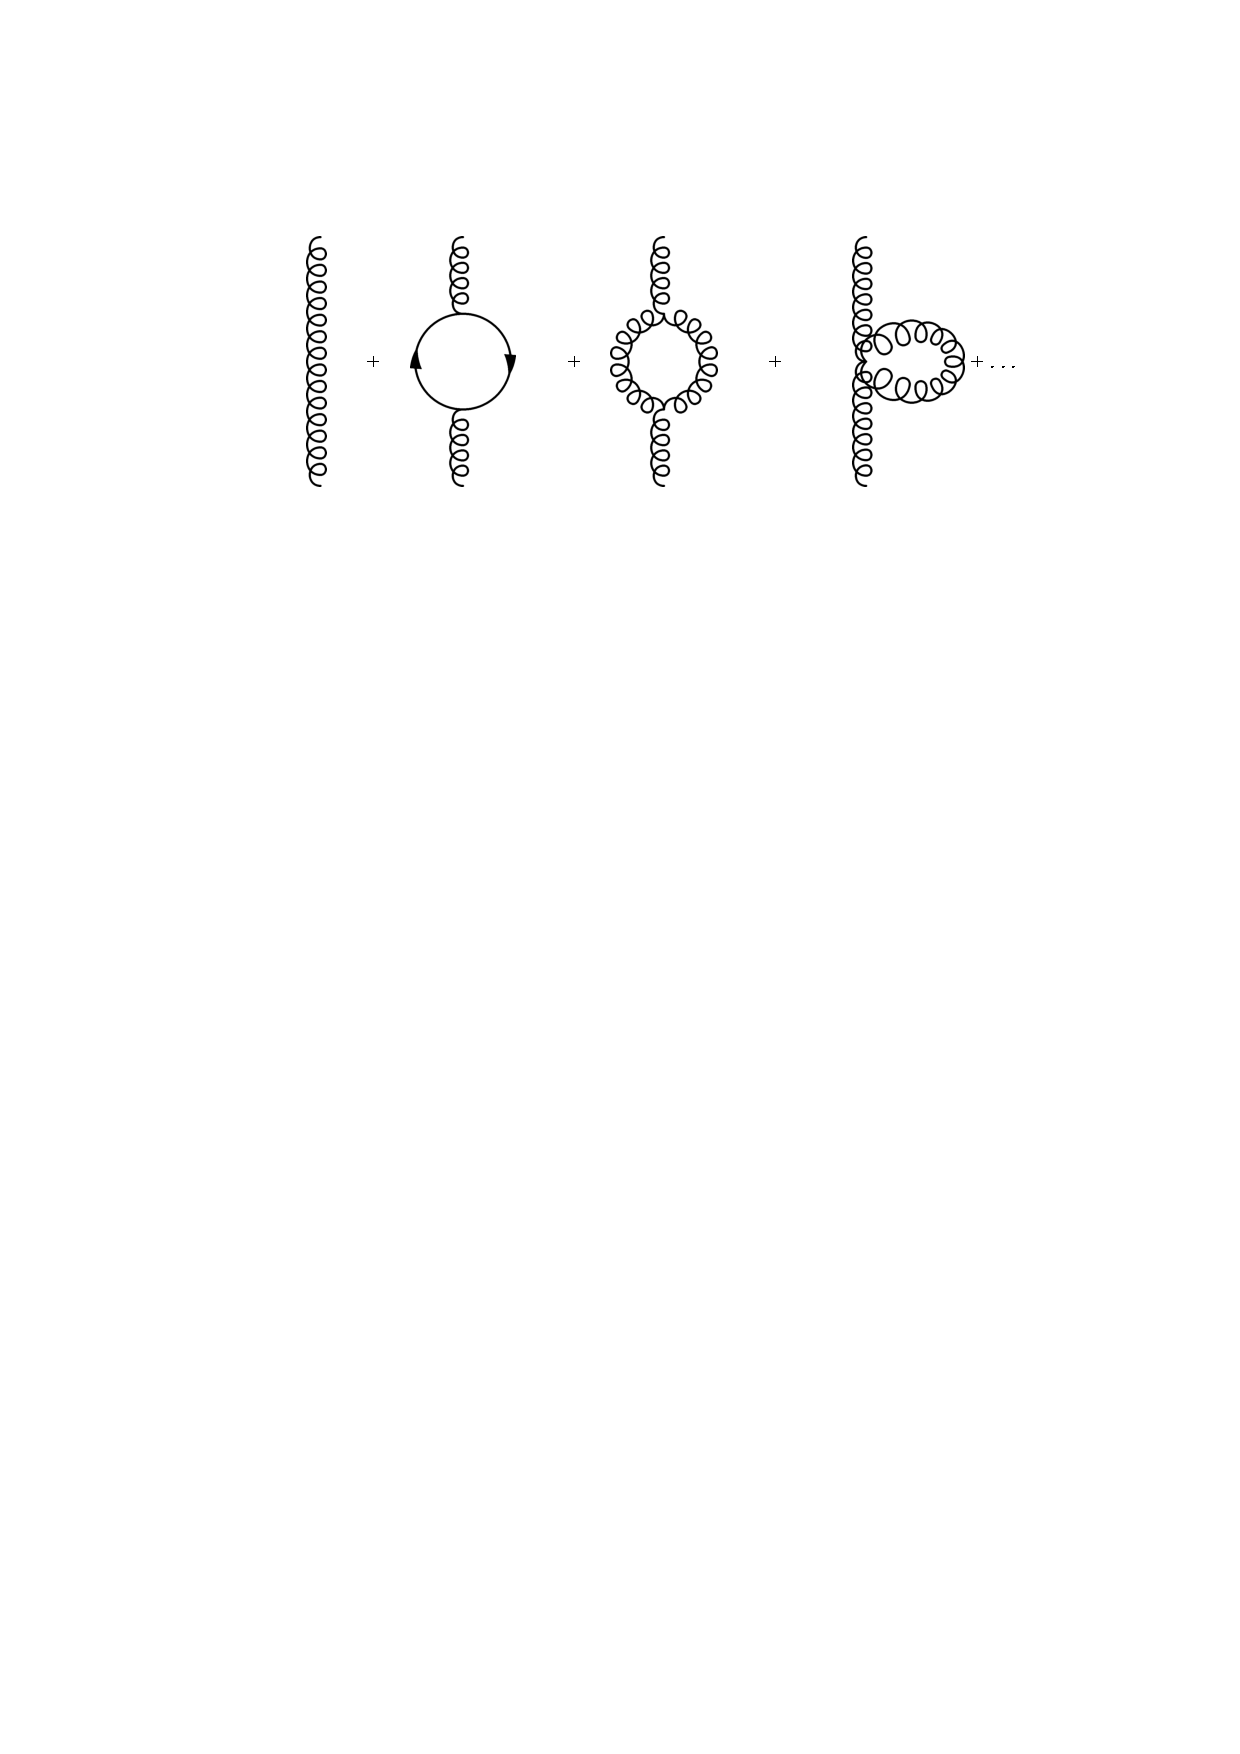
\includegraphics[width=0.7\linewidth, angle=0]{figs/Theory/qcd_gluon_loop.pdf}
  \end{center}
  \caption[A schematic showing the gluon propagator with the additional first order loops.]
  {A schematic showing the gluon propagator with the additional first order loops~\cite{det-thesis_kate}.}
  \label{fig:theo-qcd_gluon}
\end{figure}

To avoid these divergences, there is a well accepted mathematical tool, known as renormalisation,
where one effectively re-scales the fields in the Lagrangian~\cite{theo-qcd}.
Renormalisation is done such that the divergences are removed
when performing perturbative calculations of QCD.
This leads to a dependence of the strong coupling constant, $\alpha_S$, on the renormalisation scaled used, $\mu_R$,
an effect known as the running of $\alpha_S$.
To get an effective strength of the strong interaction in any given process,
the value of $\mu_R$ is set as the scale of the momentum transfer, $Q$, of the process.
%%which is the natural choice for the process.
%$\alpha_S($\mu_R \sim Q^{2}$).
The running of $\alpha_{S}$ can be measured through experimental observation;
Figure~\ref{fig:theo-qcd_running} shows the measured values of $\alpha_S$
as a function of the energy scale, $Q$, in a range of experiments.

\begin{figure}[!hbt]
  \begin{center}
    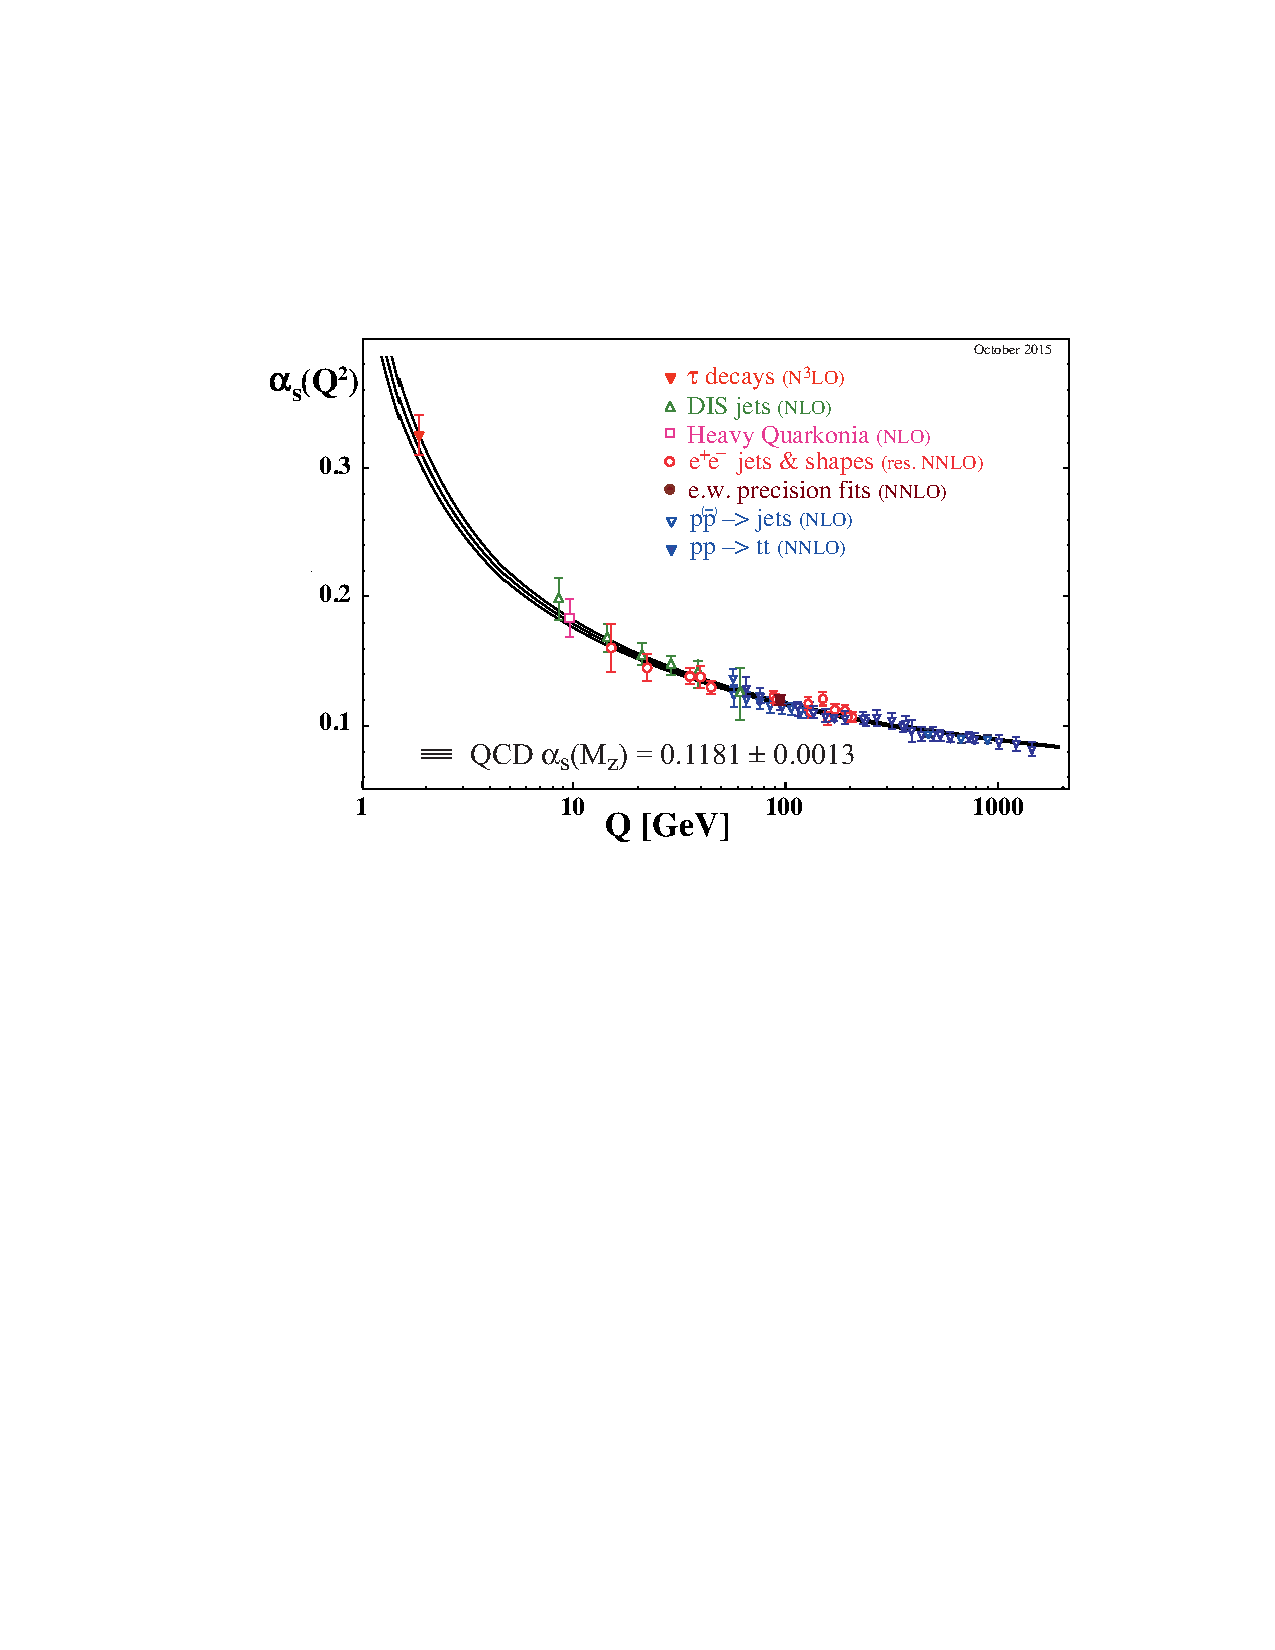
\includegraphics[width=0.7\linewidth, angle=0]{figs/Theory/qcd_running.pdf}
  \end{center}
  \caption[Summary of measurements of $\alpha_S$ as a function of the energy scale, $Q$.]
          {Summary of measurements of $\alpha_S$ as a function of the energy scale, $Q$.
            The respective degree of QCD perturbation theory used in the extraction of $\alpha_S$ is indicated in brackets
            (NLO: next-to-leading order; NNLO: next-to-next-to leading order; res. NNLO: NNLO matched with resummed next-to-leading logs; N3LO: next-to-NNLO)~\cite{theo-qcd}.}
  \label{fig:theo-qcd_running}
\end{figure}

There are three features of Figure~\ref{fig:theo-qcd_running} that should be noted.
Firstly, the size of $\alpha_S$ is generally large compared to $\alpha_{EM}$;
this means that, depending on the energy scale, the strong force is typically stronger than the EM force by one or two orders of magnitude.
Secondly, at high energies/small distances the strong force becomes relatively weak, this phenomenon is known as
\textit{`asymptotic freedom'}.
At these energy scales, perturbative expansions of QCD are possible.
Finally, at low energies/large distances the strong force is exceptionally strong.
As a result, if two interacting quarks become separated by a large distance then it becomes energetically favourable to
pair-produce $q\bar{q}$ pairs from the vacuum until a colour neutral object can be formed.
Therefore quarks are not observed in isolation, but instead quarks form colour neutral hadrons; this feature of QCD is known as \textit{`confinement'}.
At low-energy scales perturbative expansions of QCD are not possible.

\subsection{Hadronic Jet Formation}
\label{sec:theo-qcd_jets}

It is common in hadronic colliders that a high-momentum quark or gluon will be produced in the final-state
\footnote{An example of this is dijet production, as will be described in Section~\ref{sec:theo-qcd_dijet}.}.
However, due to the effect of quark confinement described above, an isolated quark or gluon will not be observed.
Instead a stream of energetic, collimated hadrons will be formed, known as a hadronic jet.
Hadronic jet formation occurs through two distinct processes; parton-shower and hadronisation.

\begin{itemize}[leftmargin=*]
  
\item\textbf{Parton Shower:}

  The high-energy final-state quark or gluon will split into a $qg$ or $q\bar{q}$ pair respectively.
  The resulting quarks and gluons will also undergo splitting to form more partons,
  which in turn can split. This process continues to form the parton shower.
  Due to relativistic effects, each splitting will generally be at a small opening angle in the lab-frame
  and as such the partons will be highly collimated in the direction of the initial parton.
  The parton shower process occurs at high energy such that the value of $\alpha_S$ is small
  and thus perturbative expansions of QCD can be used to perform calculations.
  However, at each step of the splitting the energy of the partons decreases
  and thus the value of $\alpha_S$ increases.\vspace{0.5em}
  
\item\textbf{Hadronisation:}
  
  When the energy scale becomes small
  \footnote{This is generally defined as small relative to the hadronic scale, $\Lambda$, which is typically a few hundred MeV},
  $\alpha_S$ becomes large such that the dominant QCD effect is quark confinement.
  Therefore, the quarks and anti-quarks produced in the parton shower form hadrons.
  The hadrons are colour neutral objects, meaning that stable hadrons that do not interact through QCD will be formed
  \footnote{Some unstable hadrons, such as a $\Delta^{++}$, may be initially formed in the process but these will decay rapidly through the strong interaction.
    In addition, some hadrons might not be stable under the weak interaction, such as a Kaon, but the time-scale of their decays will be much larger.}.
  The hadronisation process occurs at large values of $\alpha_S$ so cannot be calculated using perturbative expansions;
  models such as the string model~\cite{theo-qcd_jet_string} and the
  cluster model~\cite{theo-qcd_jet_cluster} are used to simulate hadronisation.

\end{itemize}
  
The end result of the hadronisation process is a set of collimated stable hadrons,
known as a hadronic jet, which can be observed in an experiment.
Note that our understanding of how one goes from an initial parton to a hadronic jet is model dependant,
for example there is a choice of hadronisation model.
Hence, in experiment this dependence is removed by defining a jet in terms of observables,
such that the experimental results are model-independent and results can be reinterpreted when improved models become available
\footnote{A good explanation of why model-independent jets is desirable is found here~\cite{theo-jets_jb}}.
The details of the experimental definition of a hadronic jet is discussed in Section~\ref{sec:obj-jets}.

%\subsection{Parton shower}
%\subsection{Hadronisation}

\subsection{Dijet Production in $pp$ Collisions}
\label{sec:theo-qcd_dijet}

QCD dijet production is one of the most common process that occurs in proton--proton colliders.
QCD dijet production occurs when the two protons interact through QCD to give two quarks or gluons in the final state;
the frequency of this interaction is described by the hadronic cross-section, $\sigma_{had}$.
The free partons will then form hadronic jets through the processes described in Section~\ref{sec:theo-qcd_jets}.
Figure~\ref{fig:theo-qcd_dijet_feynman} shows the Feynman diagram of
dijet production in a proton--proton collision through the $qg \to qg$ channel.

\begin{figure}[!hbt]
\vspace{-1em}
  \begin{center}
    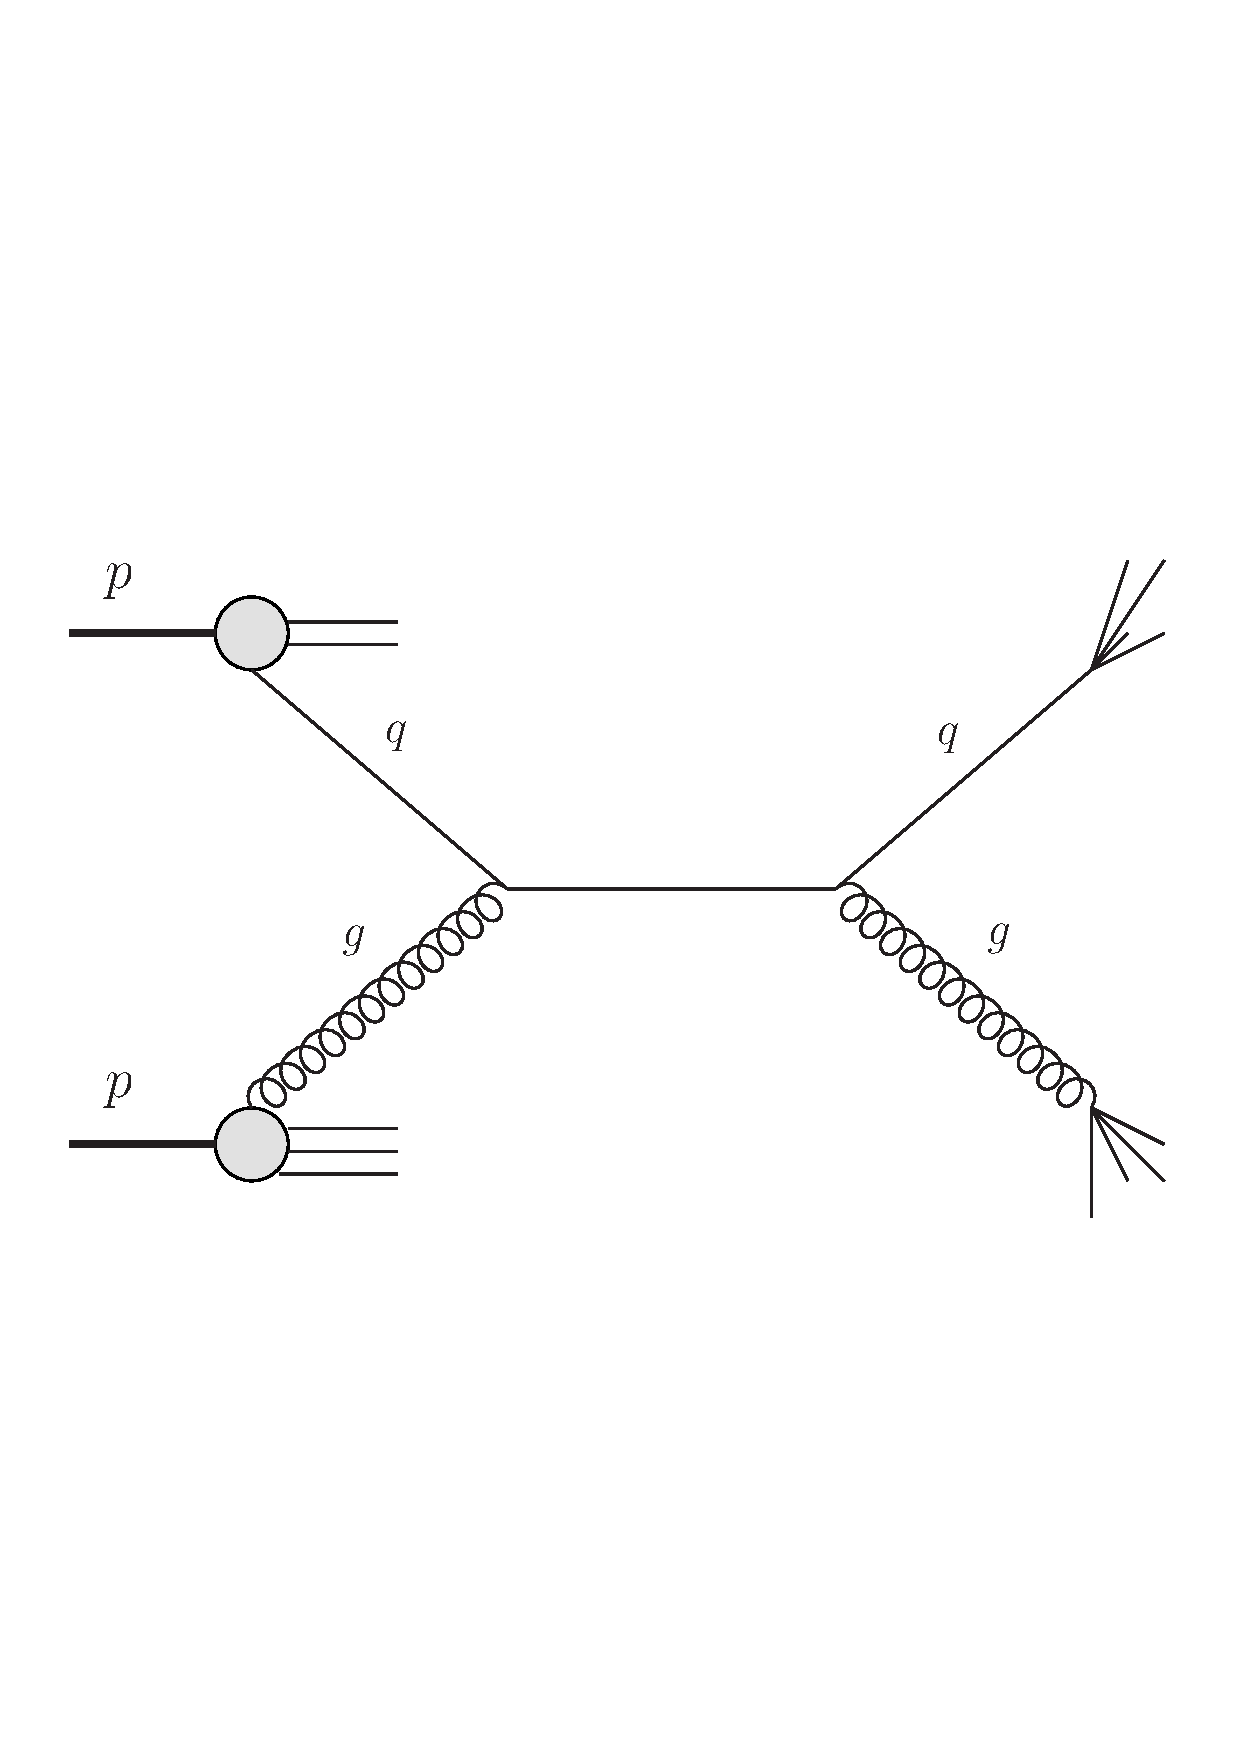
\includegraphics[width=0.65\linewidth, angle=0]{figs/Theory/qcd_dijet_feynman.pdf}
  \end{center}
%  \caption[Three feynman diagrams illustrating the parton level scatter process in dijet production at the LHC.]
  %          {Three feynman diagrams illustrating the parton level scatter process in dijet production at the LHC~\cite{theo-qcd_dijet_feynman}.}
  \vspace{-1em}
  \caption[A Feynman diagram showing dijet production in a proton--proton collision through the $qg \to qg$ channel.]
          {A Feynman diagram showing dijet production in a proton--proton collision through the $qg \to qg$ channel. Adapted from~\cite{theo-qcd_dijet_feynman}.}
          \label{fig:theo-qcd_dijet_feynman}
\vspace{-1em}
\end{figure}

To calculate the hadronic cross-section, $\sigma_{had}$, in a proton--proton collision,
two elements are separated out in a process called \textit{`factorisation'}.

The first element is the \textit{`parton-level cross-section'}, $\hat{\sigma}$, which is the cross-section of
two partons from the proton ($p_i$ and $p_j$) scattering to give two final state partons ($p_k$ and $p_l$).
In Figure~\ref{fig:theo-qcd_dijet_feynman}, $p_i$ and $p_j$ represent the incoming $q$ and $g$ and $p_k$ and $p_l$ represent the the outgoing $q$ and $g$.
The parton-level cross section is discussed further in Section~\ref{sec:theo-qcd_dijet_xs}.
%This is effectively the central part of the Feynman diagram in Figure~\ref{fig:theo-qcd_dijet_feynman}.

The second element is the \textit{Parton Distribution Function} (PDF), $F_i(x_i)$,
which gives the number density of a specific parton, $p_i$, with momentum fraction, $x_i$, in a proton.
Momentum fraction is defined as the fraction of the proton's total momentum that the parton is carrying, $x = p_{\text{parton}}/p_{\text{proton}}$.
%The number density affects the overall cross-section, as it changes the probability that a specific parton
%can form the initial parton propagators.
This part of the interaction is indicated by the circles on the left of the Feynman diagram in Figure~\ref{fig:theo-qcd_dijet_feynman}.
Further details on PDFs is found in Section~\ref{sec:theo-qcd_pdf}.

The elements are combined to calculate $\sigma_{had}$;
\begin{equation}
%  \sigma(p_1p_2\to q/g_k q/g_l) = \int dx_1 dx_2 F_1(x_1,\mu^2_F)F_2(x_2\mu^2_F) \sigma(q/g_1,q/g_2, \alpha_s(\mu^2_R),Q^2/\mu^2_F,Q^2/\mu^2_R)
  \sigma_{had} = \sum_{i,j,k,l} \int dx_i\hspace{0.3mm} dx_j \hspace{1mm} F_i(x_i,Q^2)\hspace{1mm}F_j(x_j,Q^2)\hspace{1mm}\hat{\sigma}(p_i, p_j\to p_k p_l)
\end{equation}
where there is an integral over all possible values of momentum fractions $x_i$ and $x_j$,
a sum over all possible initial partons from the two protons labelled $i$ and $j$,
and a sum over all possible final-state partons labelled by $k$ and $l$
\footnote{The final state sums do not include top-quarks because, as will be discussed in Section~\ref{sec:theo-ttbar}, they do not form regular jets. 
  In addition, due to its heavy mass, the top-quark is heavily suppressed in the PDFs so can be ignored in the sum over initial partons.}.
$Q^2$ is the energy scale of the collision.

\noindent
With the two elements separated we can discuss each separately.

\subsubsection{Parton-level Cross-Section}
\label{sec:theo-qcd_dijet_xs}

To describe the parton-level cross-section, some useful variables must first be defined.
The first is the invariant mass of the outgoing partons, $m_{kl}$, which is given in terms of the four-momentum of the two partons;
\begin{equation}
  m_{kl}^2 = (p^\mu_k + p^\mu_l)^2  
\end{equation}
\noindent
Then there are two related angular variables, $y^*$ and $\theta^*$,
defined in terms of the rapidities of the outgoing partons, $y_k$ and $y_l$;
\begin{equation}
  y^* = (\frac{y_k - y_l}{2})
\end{equation}
\begin{equation}
  cos(\theta^*) = \tanh(y^*)
\end{equation}
\noindent
Finally the Mandelstam variables are defined as, %generally used to describe a 2$\to$2 particle scatter event, 
\begin{equation}
  \hat{s} = m_{kl}^2, \hspace{3mm}  \hat{t} = -\hat{s}\hspace{1mm}(1 - \cos{\theta^*}), \hspace{3mm} \hat{u} = - \hat{s}\hspace{1mm}(1+\cos{\theta^*})
  \label{eqn:theo-mandy}
\end{equation}
The Mandelstam variables represent the square of the 4-momentum of the propagator in a 2$\to$2 particle scatter event
for an s, t or u-channel Feynman diagram respectively.

\noindent
The parton-level differential cross-section of incoming partons $i$ and $j$ scattering to give
outgoing partons $k$ and $l$ is given in terms of the variables $\theta^*$ and $m_{kl}$~\cite{theo-qcd_xs};
\begin{equation}
  \frac{d^2 \hat{\sigma}(p_i, p_j \to p_k p_l)}{dm_{kl}^{2}\hspace{1mm}d\cos{\theta^*}} = \frac{ \pi \alpha_s^2}{2 \,  m_{kl}^2}
  \ \delta(x_i x_j s - m_{kl}^{2})\ \text{S}(ij \to kl) \hspace{1mm} \frac{1}{1+\delta_{kl}}
  \label{eq:theo-qcd_dijet_xs}
\end{equation}
where $\sqrt{s}$ is the centre-of-mass energy and $\text{S}(ij \to kl)$ is the process dependant kinematics of a $ij \to kl$ parton scatter.
The $\delta(x_i x_j s - m_{kl}^{2})$ term requires that the invariant mass of the incoming partons is same as the invariant mass of the propagator.
%The $\text{S}\nobreak(ij~\to~kl)$ for each process is given in Table~\ref{tab:theo-qcd_dijet_s}.

The $\text{S}\nobreak(ij~\to~kl)$ for each process is given in Table 1 in~\cite{theo-dijet_harris}.
All but one process can occur through a t-channel diagram and therefore the 
$\text{S}\nobreak(ij~\to~kl)$ for those processes contains a $1/\,\hat{t}\,$ or $(1/\,\hat{t})^2\,$ term.
The importance of this will be discussed in Section~\ref{sec:theo-qcd-dijet_features}.

%  \begin{table}[!hbt]
%  \begin{center}
%    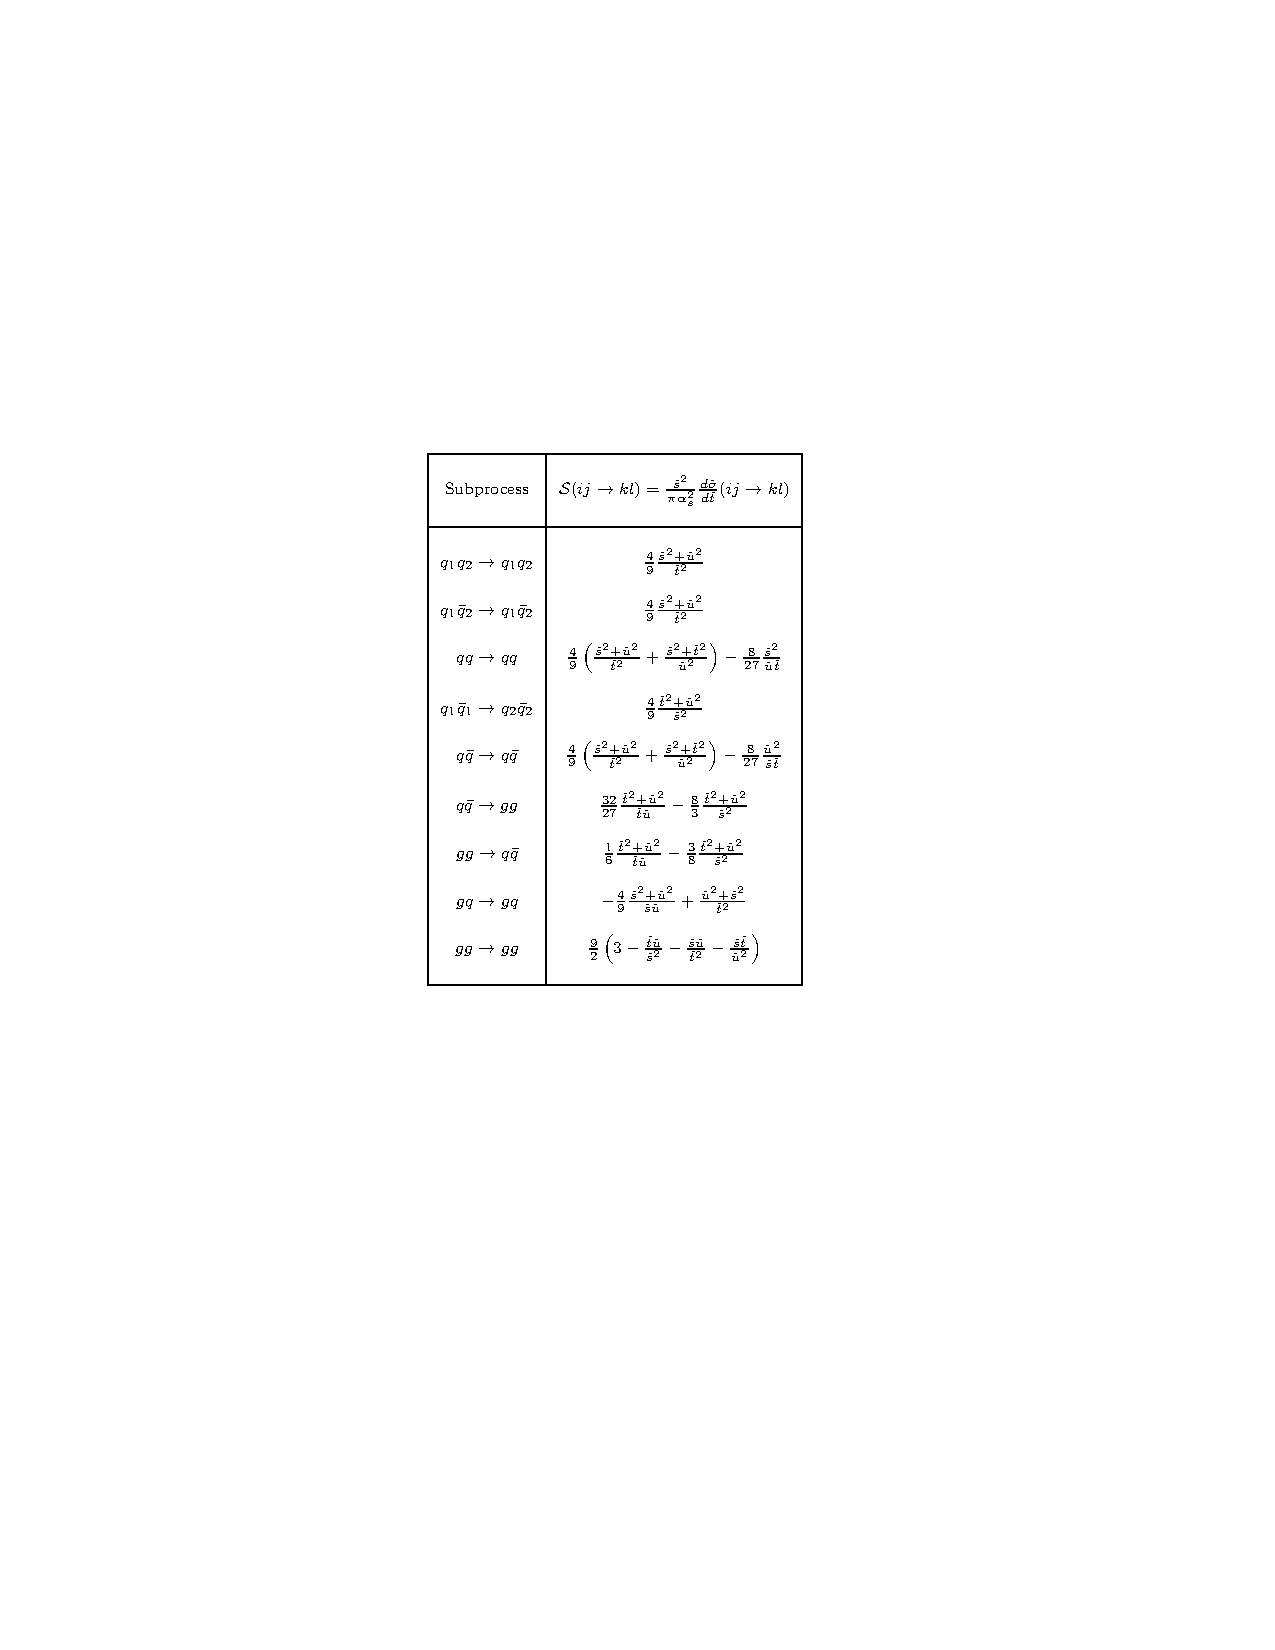
\includegraphics[width=0.5\linewidth, angle=0]{figs/Theory/qcd_dijet_stable.pdf}
%  \end{center}
%  \caption[A table showing $\text{S}(ij \to kl)$, the process dependant part of the parton cross-section, for all possible processes.]
%          {A table showing $\text{S}(ij \to kl)$, the process dependant part of the parton cross-section, for all possible processes.
%            The indices refer to quark flavour, if no indices are used then the same flavour is used for all quarks in that process. Taken from Table 1 of~\cite{theo-dijet_harris}. }
%  \label{tab:theo-qcd_dijet_s}
%\end{table}

\subsubsection{Parton Distribution Functions}
\label{sec:theo-qcd_pdf}

%A naive model of the proton contains two up-quarks and a down-quark,
%known as valence quarks, each carrying $\frac{1}{3}$ of the proton's momentum.
%However, QCD interactions within the proton mean that gluons can be emitted from the valence quarks
%and $q\bar{q}$ pairs can be produced from the emitted gluons.
The proton contains two $u$-quarks and a $d$-quark, known as valence quarks, and a sea of quarks and gluons created
through QCD interactions, such as gluons being emitted from the valence quarks and $q\bar{q}$ pairs being produced from the emitted gluons.
%The valence quarks will typically carry a lower fraction of the proton's momentum.
% typically carrying a large fraction of the proton's momentum.

Parton Distribution Functions (PDFs) give the number density of a specific parton $p_i$ in a proton $P_i$
for a given momentum fraction $x_i$ and energy scale, $Q$.
Due to the large value of $\alpha_S$ in the proton, QCD cannot be considered in perturbative expansions and as such the PDFs cannot be calculated directly.
Instead the PDFs can be measured by combining a range of experimental scattering results.
In particular, strong constraints on the PDFs come from deep inelastic scattering using $ep$ colliders, such as HERA~\cite{theo-qcd_hera};
the strong constraints are due, in part, to there only being one parton in the collision allowing direct access to the PDFs in a cross-section measurement.

%%%%%%%%%  Note Laurie %%%%%%%%%
%%%% In general one would do e- + p -> e- + jet at HERA
%%%% For sensitiviy to certain versions would could vary the analysis
%%%% For example  e- + s -> mu_e + c->D meson -> mu_e + (jet with muon).

\begin{figure}[!b]
  \begin{center}
    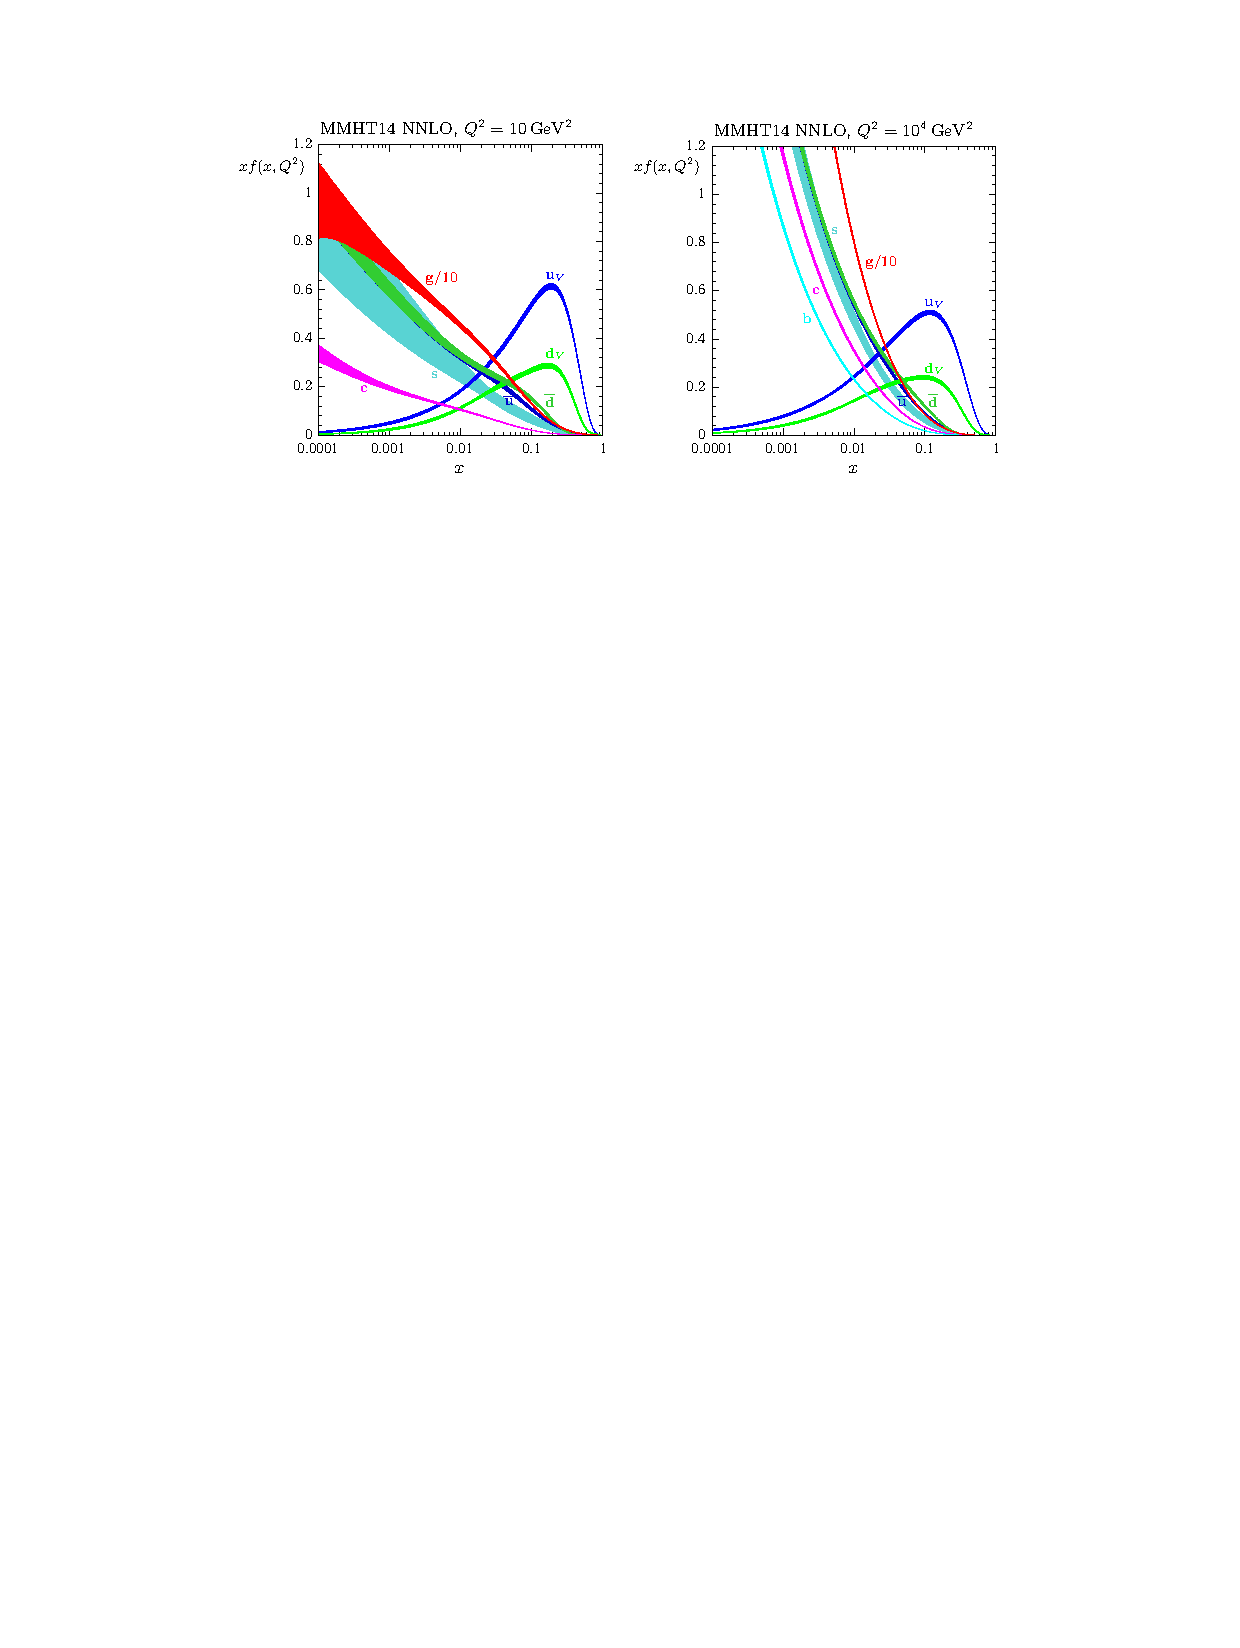
\includegraphics[width=1\linewidth, angle=0]{figs/Theory/qcd_pdf.pdf}
  \end{center}
  \caption[MMHT2014 NNLO PDFs at $Q^2$ = 10 $\text{GeV}^2$ and $Q^2$ = $10^4$ $\text{GeV}^2$, with associated 68\% confidence-level uncertainty bands.]
  {MMHT2014 NNLO PDFs at $Q^2$ = 10 $\text{GeV}^2$ and $Q^2$ = $10^4$ $\text{GeV}^2$, with associated 68\% confidence-level uncertainty bands~\cite{theo-qcd_pdf}.}
  \label{fig:theo-qcd_pdf}
\end{figure}


Figure~\ref{fig:theo-qcd_pdf} shows the $x\hspace{0.3mm}F(x,Q^2)$ for a $Q^2$ of 10 and $10^4$ $\text{GeV}^2$
from the MMHT2014 PDF set~\cite{theo-qcd_pdf}.
The various coloured lines represent the PDF for each of the different partons.
It shows that as $x$ increases the values of the PDF for the sea quarks and gluons will fall smoothly;
this is because it is energetically unfavourable to produce high momentum gluons or $q\bar{q}$ pairs.
The fall in the PDFs with respect to $x$ is particularly notable for the gluon which is the dominant contribution at large $Q^2$ and at low $x$.
The PDFs of the valence quarks, $u_v$ and $d_v$, have a peak value around $x \sim \frac{1}{3}$, and then fall off rapidly at higher $x$.
This shape is caused as at leading-order the quarks share the momentum equally, but higher-order QCD effects smear this distribution.


%If one considered the proton in the initial naive model of the proton then we find the PDFs of valence quarks as delta peaks at exactly $\frac{1}{3}$
%with amplitude of $\frac{2}{3}$ and $\frac{1}{3}$ for the $u$ and $d$ quark respectively;
%however, QCD interactions have smeared this peak to what is observed.

\subsubsection{Features of the QCD Dijet Production}
\label{sec:theo-qcd-dijet_features}

From the two factorised elements discussed above,
%shown in Section~\ref{sec:theo-qcd_dijet_xs}~and~\ref{sec:theo-qcd_pdf}.t
there are four important features of the dijet hadronic cross-section
that are significant when forming the di-$b$-jet search strategy.% in Chapters~\ref{sec:evt}~and~\ref{sec:bkg}.

\begin{itemize}[leftmargin=*]
\item\textbf{Large cross-section :}\\
  The strong coupling constant $\alpha_s$ is large meaning that the dijet cross-section is large.
  Therefore QCD dijet production is the dominant background in di-$b$-jet searches.\vspace{0.5em}
  
\item\textbf{Smoothly falling with respect to $m_{kl}$ :}\\
  QCD dijet production will be smooth and monotonically decreasing
  with respect to $m_{kl}$ as a result of three factors.
  Firstly, the cross section has a $1/m_{kl}^{2}$ term.
  Secondly, as shown in Section~\ref{sec:theo-qcd_dijet_running},
  $\alpha_S$ will smoothly decrease with increasing $Q$, which in this case is correlated with $m_{kl}$.
  Finally, as $m_{kl}$ increases then the momentum fraction of the \mbox{proton, $x$,} required to create
  the dijet event will also increase.
  As shown in Figure~\ref{fig:theo-qcd_pdf}, the parton distribution functions are generally falling 
  with respect to $x$, which will lead to falling behaviour in the hadronic cross-section.
  \vspace{0.5em}
  
\item\textbf{Increased production at large values of $|y^*|$ :}\\
  A discussed in Section~\ref{sec:theo-qcd_dijet_xs}, all but one of the $\text{S}(ij \to kl)$ terms
  contains a $1/\hat{t}$ or $(1/\,\hat{t})^2\,$ contribution from t-channel Feynman diagrams.
  These terms will become large when $\hat{t} \to 0$ which, from the definition of $\hat{t}$ in Equation~\ref{eqn:theo-mandy},
  occurs when $\cos{\theta^*} \to 1$.
  This means that QCD dijet production is increased large values of $|y^*|$.
  \vspace{0.5em}
  
\item\textbf{Preference of light-flavour quarks:}\\
  Most $ij \to kl$ processes that produce heavy flavour quarks ($c$ or $b$),
  with the exception of $q \bar{q} \to b\bar{b} \ (\text{or}\ c\bar{c})$ and $g g \to b\bar{b} \ (\text{or}\ c\bar{c})$,
  require a heavy flavour quark to be one of the initial partons.
  Figure~\ref{fig:theo-qcd_pdf} shows the heavy flavour quarks are suppressed in the PDFs relative to the other partons.
  Therefore, dijet events will be dominated by jets initiated by gluons or light-quarks ($u$, $d$ or $s$).
 
\end{itemize}

Finally, it should be noted that the above description of the QCD dijet production is not complete;
only considered tree-level diagrams have been considered, but there also exists higher-orders diagrams.
Related to that issue is the occurrence of initial state and final state radiation, known as ISR and FSR respectively.
ISR is when an additional parton is radiated off the incoming parton and FSR is when an additional parton is radiated off an outgoing parton.
ISR and FSR can lead to additional jets in an event, creating a multi-jet event.

In addition, there is also the Underlying Event (UE) which effectively comprises of the remnants of the proton not used in the hard-scatter.
The UE will mostly be hadronic activity and as a result can lead to additional jets in the event, again creating a multi-jet event.

\subsection{A Special Case: $t\bar{t}$}
\label{sec:theo-ttbar}

The top-quark is a special case when discussing the formation of jets from quarks,
due to two properties of the top quark which are distinctive.
Firstly, due to the large suppression of decays from the 3rd generation in the CKM matrix,
the top quark decays to a $b$-quark and a $W$-boson with a branching ratio of close to~1.
Secondly, the top quark is much heavier than the bottom quark
meaning that the decay to a $b$-quark is very energetically favourable.
Therefore, the top-quark decays on a shorter time-scale than parton shower process
resulting in two separate objects; the $W$-boson and the hadronic jet.
%\footnote{If the top-quark has a large-$p_T$ then the resulting $W$-boson and jet can merge.}.

As in dijet production, $t\bar{t}$ pairs can be pair-produced in proton--proton collisions through QCD interactions.
The two top quarks will decay into two $W$-bosons and two jets containing $b$-quarks.
One mode of $t\bar{t}$ decay is when one $W$-boson decays into a $l^+~\nu_l$ pair and the other into a $l^{-}~\bar{\nu_l}$ pair.
This is known as a di-lepton $t\bar{t}$ event, a Feynman diagram showing an example of a di-lepton $t\bar{t}$ event is shown in
Figure~\ref{fig:theo-ttbar} \footnote{ This figure shows the $q\bar{q}$ mode of $t\bar{t}$ production. The $gg$ mode is the dominant at the LHC}.

\begin{figure}[!hbt]
  \begin{center}
    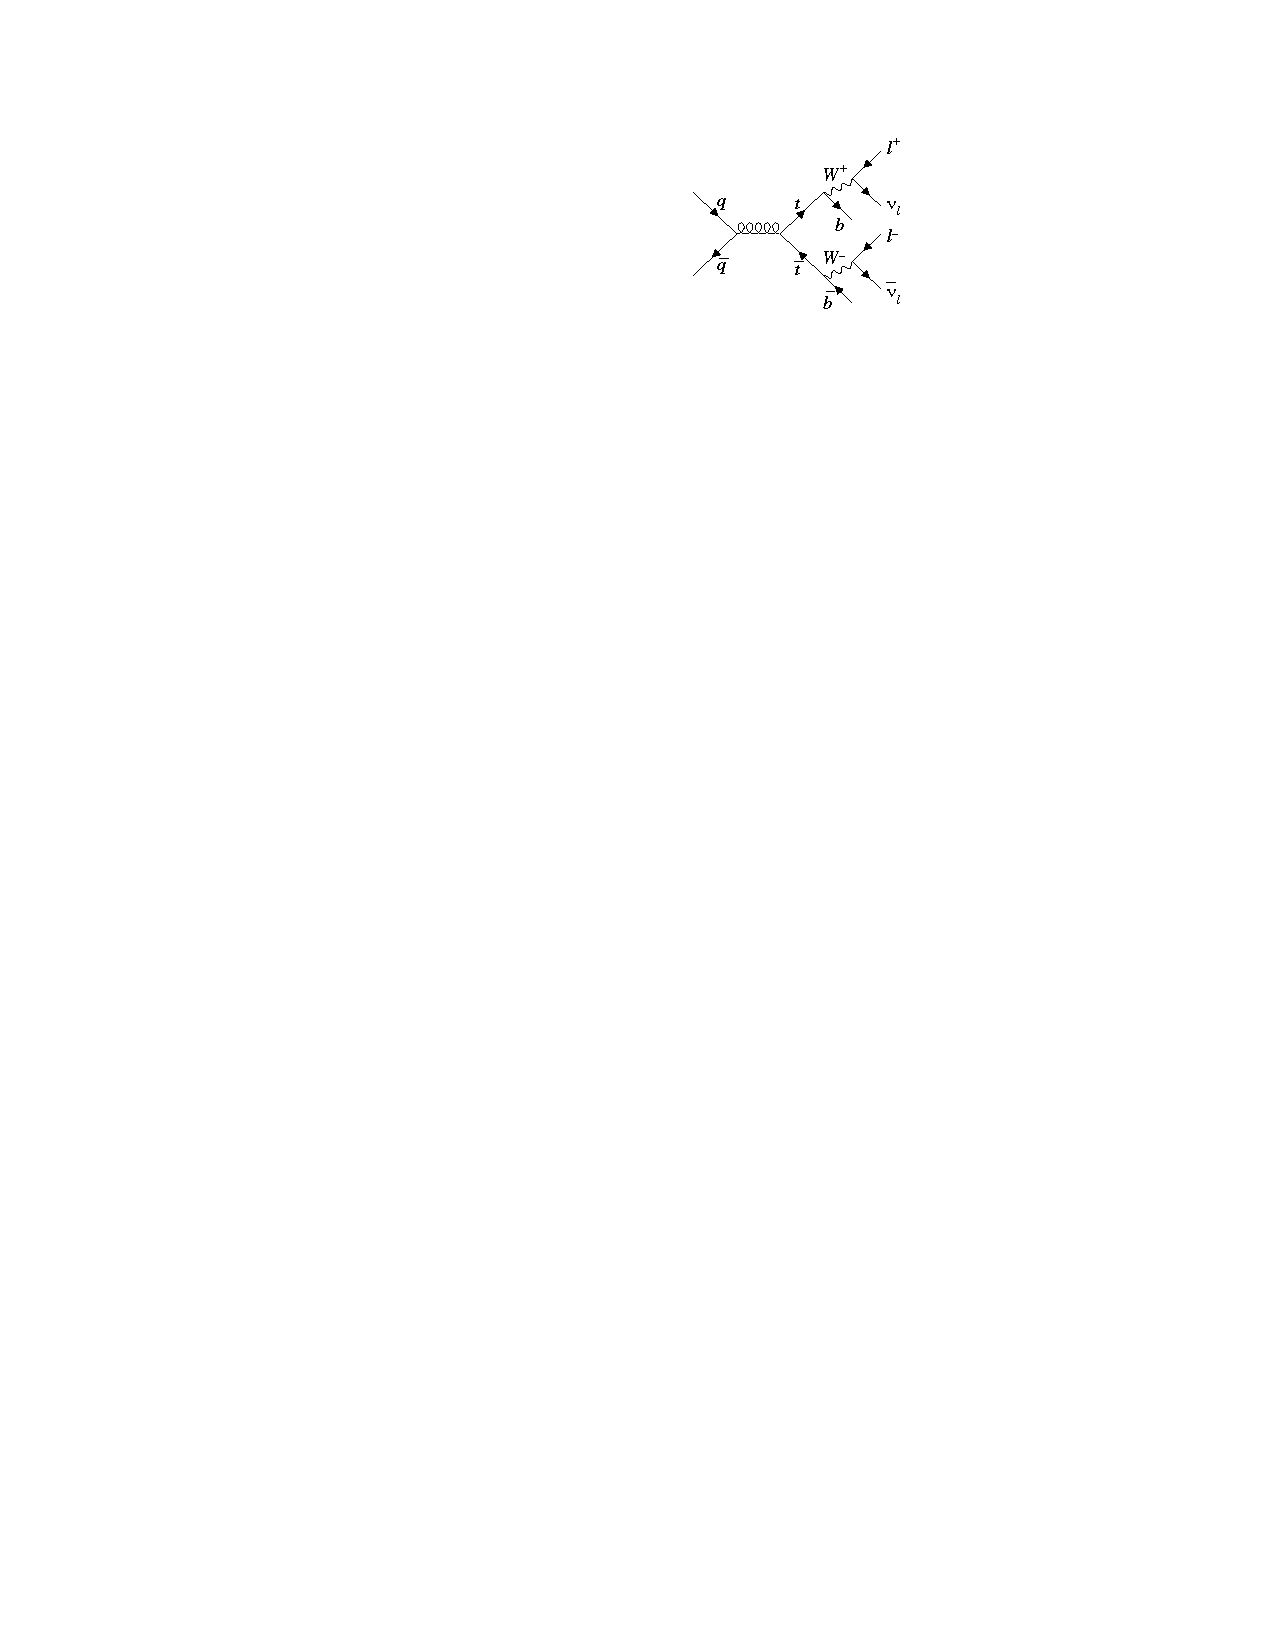
\includegraphics[width=0.6\linewidth, angle=0]{figs/Theory/ttbar.pdf}
  \end{center}
  \vspace{-1em}
  \caption[A Feynman diagram showing an example of a di-lepton $t\bar{t}$ event.]
          {A Feynman diagram showing an example of a di-lepton $t\bar{t}$ event~\cite{theo-ttbar_feyn}.}
          \label{fig:theo-ttbar}
  \vspace{-1em}
\end{figure}

Di-lepton $t\bar{t}$ forms a distinct experimental signature.
In particular, the case of opposite flavour di-lepton $t\bar{t}$, where the two leptons have different flavours, is very distinct
as this can only be caused by two separate weak-decays.
%which would typically be suppressed,
%but here the large mass of the top overcomes this suppression.
In addition we have two jets formed from $b$-quarks, which can be observed.
The distinct signature of di-lepton $t\bar{t}$ events and the fact that the top-quark nearly always decays to a $b$-quark
means that this decay topology is often used to obtain a pure sample of jets containing $b$-quarks,
as will be done in Section~\ref{sec:obj-bjets_calib}~and~\ref{sec:trig-bjet_eff}.

\newpage
\section{Beyond Standard Model Physics}
\label{sec:theo-bsm}

The preceding sections of this chapter described the Standard Model and some of its successes.
%such as the prediction of the Higgs boson and the ability to describe complex phenomena such as dijet production.
However, the Standard Model is known to be an incomplete picture of the universe.
This section will present some of the key deficiencies of the Standard Model demonstrating that Beyond Standard Model (BSM) physics is required
and discuss some proposed BSM models that motivate the analyses shown in this thesis.

\subsection{Motivations}

The motivations for BSM physics listed in this section
describe only a subset of deficiencies of the Standard Model,
with a focus on the most important missing parts and
those that motivate models searched for in this thesis.

\subsubsection{Gravity}

When listing forces in Section~\ref{sec:theo-sm_forces}, we made no reference to gravity.
This is because our description of gravity, Einstein's General Theory of Relativity,
has not been successfully merged with the Standard Model in a so-called `Quantum Theory of Gravity'.
It is a clear inadequacy of the Standard Model that there is no explanation of gravity
%partly due to the fact that gravity is hard to study at the quantum-level because
%it is so much weaker than the other forces
%(of order $10^{-39}$ compared to the strong interaction) .
% \textbf{LM Fix: Reference?}.
%There have been theoretical attempts to decribe gravity such that it is comptible with the Standard Model,
%such as the Randall-Sundrum Graviton~\cite{theo-bsm_randall},
%but so far these have not been substantiated by experimental evidence.%~\cite{trig-H4b}.

\subsubsection{Dark Matter}
\label{sec:theo_bsm_dm}

%It is remarkable that the physics that describes the largest and smallest scale known,
%Astronomy and particle physics,
%are often deeply related; the prediction of Dark Matter (DM) is a great example of this.

%Astronomers are able to make observations of distant galaxies using
%EM-waves, that allows observation of Standard Model particles  
%and are have been succesful in explaining the observed galaxies in terms of the particles of the Standard Model,
%listed in Section~\ref{sec:theo-sm_particles}.
%However, due to the large masses of astronomical objects,
%astronomers also have access to observing the action of gravity.

%Astronomers are able to make observations of distant galaxies and stars
%to study their dynamics in terms of both Standard Model processes
%and, due to the large masses of galaxies, gravitational interactions.

Astronomers have been able to make the remarkable observation that
$\sim$80\% of the universe's matter must be so-called `Dark Matter'~\cite{theo-bsm_dm_peskin}.
Dark Matter are particles not described by the Standard Model,
so is clear evidence of Beyond Standard Model physics.
It is known that Dark Matter interacts through gravity
and can only interact weakly, if at all, with the Standard Model,
otherwise we would have already observed it through interactions with Standard Model particles .

The evidence for Dark Matter comes from many separate astronomical observations:
such as studies of
galaxy rotation curves,
the cosmic microwave background
and a collision of two clusters of galaxies known as the bullet cluster,
%and galaxies using gravitataional lensing.
A wider summary of the evidence for Dark Matter can be found here~\cite{theo-bsm_dm_evidence}.

%\begin{figure}[!b]
%  \begin{center}
%    \captionsetup[subfigure]{aboveskip=0pt,justification=centering}
%    \subcaptionbox{Visible Spectrum}{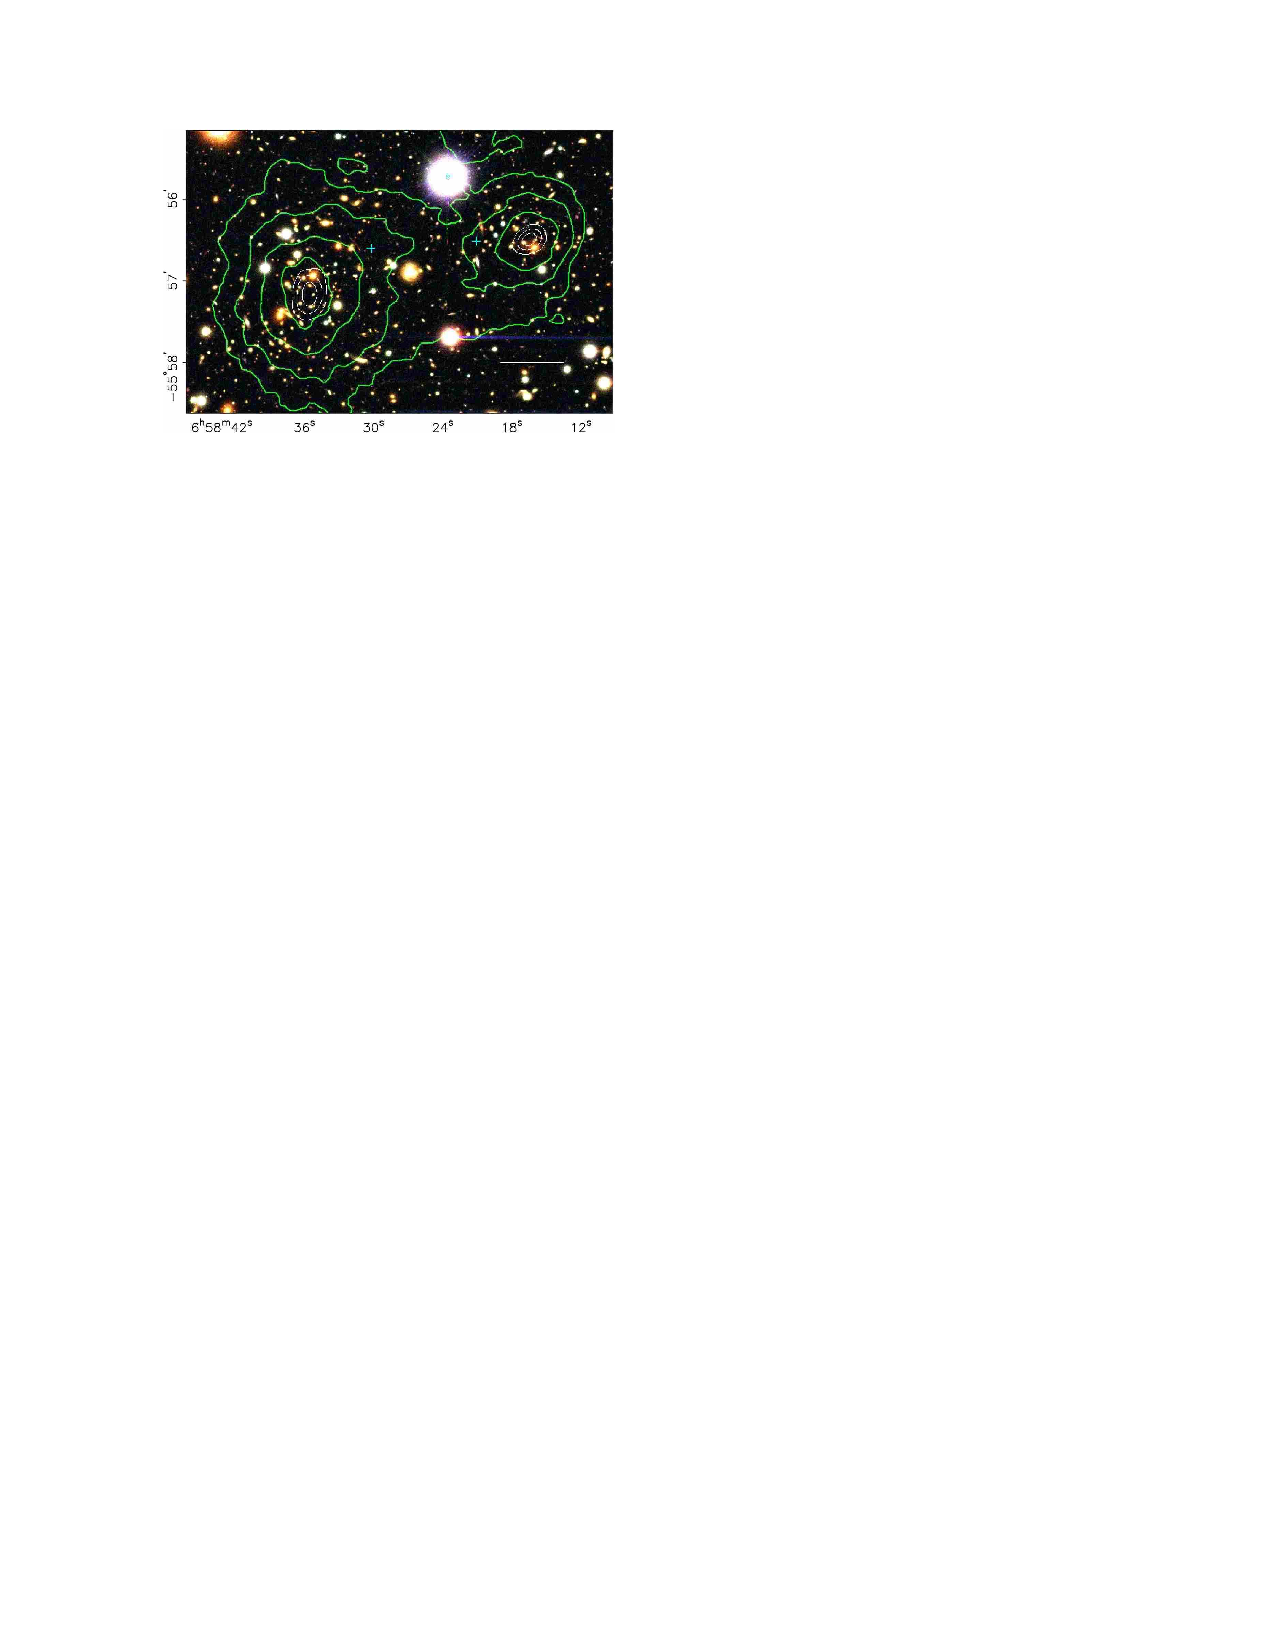
\includegraphics[width=0.48\linewidth, angle=0]{figs/Theory/bsm_gl_vis} }
%    \subcaptionbox{X-Ray Spectrum}{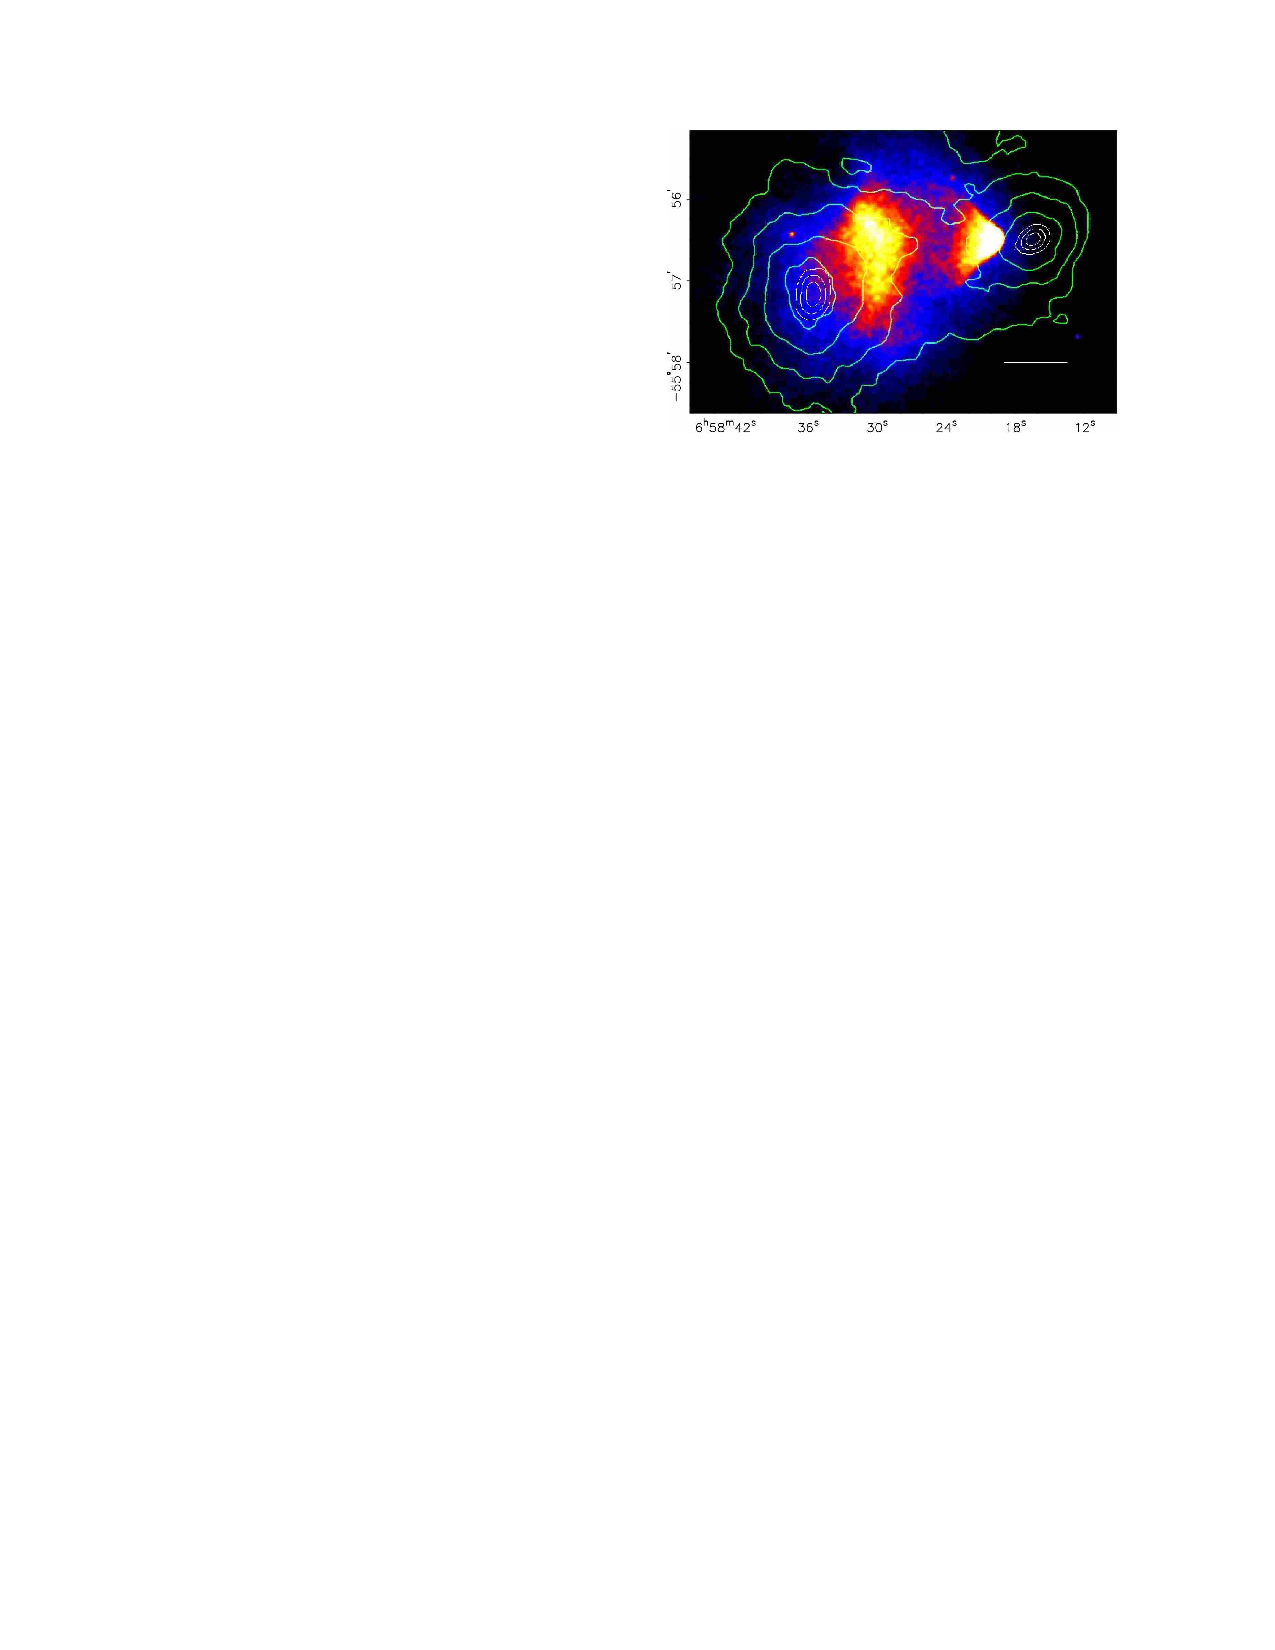
\includegraphics[width=0.48\linewidth, angle=0]{figs/Theory/bsm_gl_xray}}
%  \end{center}
%  \caption{An image of the same bullet cluster
%    (a) in the visible spectrum using the Hubble Space Telescope
%    and (b) in the X-ray spectrum using the Chandra telescope.
%    The mass density profile estimated using gravitational lensing is overlaid on both plots.}
%  \label{fig:theo-bsm_dm_gl}
%\end{figure}
%
%The cited summary provides a more rigorous explanation of the evidence than can be provided here.
%But I would like to discuss one particular bit of evidence,
%specifically measurements of bullet clusters using X-ray telescopes and gravitational lensing~\cite{theo-bsm_dm_gl}.
%Gravitational lensing occurs when the path of light from some distant astronomical source is bent by the gravitational effect of a nearer galaxy.
%Figure~\ref{fig:theo-bsm_dm_gl}(a) shows an image of a bullet cluster and the surrounding galaxies in the visible part of the light spectrum using the Hubble telescope.
%Using the gravitational lensing effect in this image one can infer the mass density profile of the bullet cluster, which is shown by the green contour lines.
%One can also observe the galaxy using an X-ray telescope,
%allowing an observation of the number density profile of Standard Model particles in a galaxy which, when hot, will emit X-ray radiation.
%Figure~\ref{fig:theo-bsm_dm_gl}(b) shows an image of the same bullet cluster in the X-ray part of the light spectrum using the Chandra telescope;
%the mass density profile estimated using the visible spectrum has again been overlaid.
%One can see that the mass density profile of the bullet cluster is inconsistent with the
%number density profile of the Standard Model particles from the X-ray telescope.
%Hence one can conclude that there must be additional Dark Matter particles in this bullet cluster
%causing the shift in the mass density profile.

Furthermore, it is believed the Dark Matter couples to the Standard Model.
This is required in many models of Dark Matter~\cite{theo-bsm_dm_feng} to explain the
observed relative abundance of Dark Matter particles in the universe.
As a result this means that there may be some yet unknown mechanism that couples to both Dark Matter and
Standard Model particles; this mechanism is referred to as a Dark Matter mediator.

%The evidence for such a statement stems from the observed relative abundance of Dark Matter particles in the universe.
%The most common method of explaining the abundance
%, known as 'freeze-out',
%argues that in the early and hot universe Dark Matter and Standard Model particles
%freely interacted such that they were in thermal equilibrium.
%As the universe expanded and cooled this interaction was suppressed
%and the number density of Dark Matter was fixed at the value we observe today~\cite{theo-bsm_dm_feng}.
%The most common method of explaining the abundance is by postulating that
%DM and SM particles were produced in the same abundance in the Big Bang,
%and in the early hot and dense universe they could interact freely such that they are in thermal equilibrium.
%As the universe begins to cool and expand this number density will fall in equilibrium with the SM particles.
%However, at some point the universe is sufficiently cool that this interaction becomes supressed and the
%number density of Dark Matter is fixed at the value we observe today; this process is known as 'freeze-out'.
%As a result this means that there may be some yet unknown mechanism that couples to both Dark Matter and
%Standard Model particles; this mechanism is referred to as a Dark Matter mediator.
%%%%% Note to laurie
%% => WIMP is if mediator is weak and particle is massive
%% => WIMP miracle is that freeze-out occurs at roughly right abundance with no extra work. Great news
%% => Unfortunately WIMP is starting to become very constrained (https://arxiv.org/pdf/1507.03800.pdf)
%% => So we might need other mediator models, such as the Z'.
%\textbf{Do I need to talk about the WIMP miracle; I was going to say no as I want to talk about Z' which is not the weak force as such}

\subsubsection{Hierarchy Problem}

The Hierarchy problem~\cite{theo-hierarchy} is the fact that the energy scale of the Higgs mechanism, ($M_{H}\nobreak=\nobreak125~\text{GeV}$),
is much smaller than the energy scale of gravity,
known as the Planck scale ($M_{Planck}\nobreak\sim\nobreak10^{19}~\text{GeV}$)~\cite{obj-bjets_PDG}.
This means that the energy scale of the Standard Model is very far
from the energy scale of the next known interaction, gravity.

The Hierarchy problem leads to complications in theoretical calculations, such as the that of the Higgs boson mass~\cite{theo-hierarchy}.
When calculating the Higgs boson mass one must consider
%the bare mass of the Higgs boson from the Lagrangian in addition to
radiative contributions from additional loop diagrams,
similar to the corrections considered for a gluon propagator shown in Figure~\ref{fig:theo-qcd_gluon}. %Section~\ref{sec:theo-qcd_dijet_running}.
However, these contributions are found to be of the order $\delta m_H^2 \sim \frac{1}{16\pi^2} M_{Planck}^2$\hspace{0.2mm},
orders of magnitude larger than the observed mass of the Higgs boson.
This means that some mechanism must either cancel the contributions or reduce their size.
Whilst the free parameters of the Standard Model can be chosen such that these different contributions approximately cancel out,
such fine-tuning of the parameters is hard to believe without some underlying explanation.

Instead, there are two solutions typically proposed to stabilise the effect of the loop corrections.
Firstly, one can introduce BSM physics that has loop contributions that cancel the Standard Model contributions.
For example this occurs in theories of supersymmetry~\cite{theo-bsm_susy}.
Secondly, one can introduce some BSM physics at a new energy scale
such that the loop diagram contributions are cut off at $\delta m_H^2 \sim \frac{1}{16\pi^2} M_{BSM}^2$.
If the BSM physics is on the TeV scale then this would reduce to size of the loop corrections to the scale of the Higgs boson's mass,
giving some prior belief that new physics could be found at this energy scale.
%Both solutions could result in BSM physics around the TeV scale.

\subsubsection{Generational Structure of Quarks}
\label{sec:theo-bsm_3g}

The quarks of the Standard Model have a well ordered generational symmetry.
However the generational symmetry is not perfect;
each generation is heavier than the previous one
and within the generations quarks have different masses.
In particular, the third generation of quarks is somewhat special;
the top quark is much heavier than the bottom quark
and is the heaviest particle of the Standard Model.
Furthermore, as the mass of the top quark is close mass of the Higgs boson,
the 3rd generation of quarks have a role symmetry breaking within the Higgs mechanism for some BSM models~\cite{theo-bsm_top}.

There is no good explanation of why there is generational structure in the Standard Model,
why the mass hierarchy is unsymmetric 
or why the third generation has one quark with such a large mass.
The generational structure could be a result of some underlying broken symmetry
which forms a part of a deeper theory of particle physics.
Any deeper theory explaining the generational structure could contain observable BSM particles,
and, given the special nature of the third generation,
the BSM particles could couple strongest with the third generation of quarks.

Unlike the case of Dark Matter,
the generational structure of quarks
and the special nature of the third generation is not concrete evidence of BSM physics.
But it does mean that there are motivations to be particularly interested in
searches for resonances decaying to the third generation of quarks.

\subsection{Beyond Standard Model Theories}
\label{sec:theo-bsm_models}

The previous section discussed a list of deficiencies of the Standard Model,
which makes us confident that Beyond Standard Model physics must exist.
This leads us to ask what the new theory of physics could be and
how can one obtain evidence of such a theory.

Many proposed theories of BSM physics include the addition of a new particle and,
in particular, the special nature of the third generation
\footnote{Discussed in Section~\ref{sec:theo-bsm_3g}}
means that some models of BSM predict new particles
that preferentially decay to two $b$-quarks or a $b$-quark and a gluon.
Furthermore, the Hierarchy Problem suggests that BSM physics may exist at the TeV energy-scale.
The observation of such a resonance would be evidence of BSM physics.

Two such models that predict resonances with preferential decays to $b$-quarks are discussed below.
These are used as \textit{`benchmark models'} in the analyses presented in this thesis,
where a benchmark model is a plausible signal model that is used to form and optimise a search strategy.
Furthermore the benchmark models are used to represent many models that decay to one or more $b$-quarks.

\subsubsection{$Z'$ Boson}
\label{sec:theo-bsm_zprime}

One of the most simple additions to the Standard model is that of a $U(1)'$ gauge symmetry
which would result in an additional spin-1 boson, known as the $Z'$ boson.
An additional $U(1)'$ symmetry appears in many different BSM models and is therefore a well motivated BSM extension~\cite{theo-bsm_zprime}.
The $Z'$ boson can decay to a pair of $b$-quarks, as shown in Figure~\ref{fig:theo-bsm_zprime}.
%Often theses models use the breaking of some higher gauge symmetry to give $G_{SM}~\text{x}~U'(1)^n$ gauge symmetry group,
%and thus giving additional predicting the existence of new gauge bosons in addition to the Standard Model
%\footnote{$G_{SM} = SU(3)~\text{x}~SU(2)~\text{x}~U(1)$, which is the gauge symmetry group of the Standard Model discussed in Section~\ref{sec:theo-sm}}.

\begin{figure}[!hbt]
  \begin{center}
    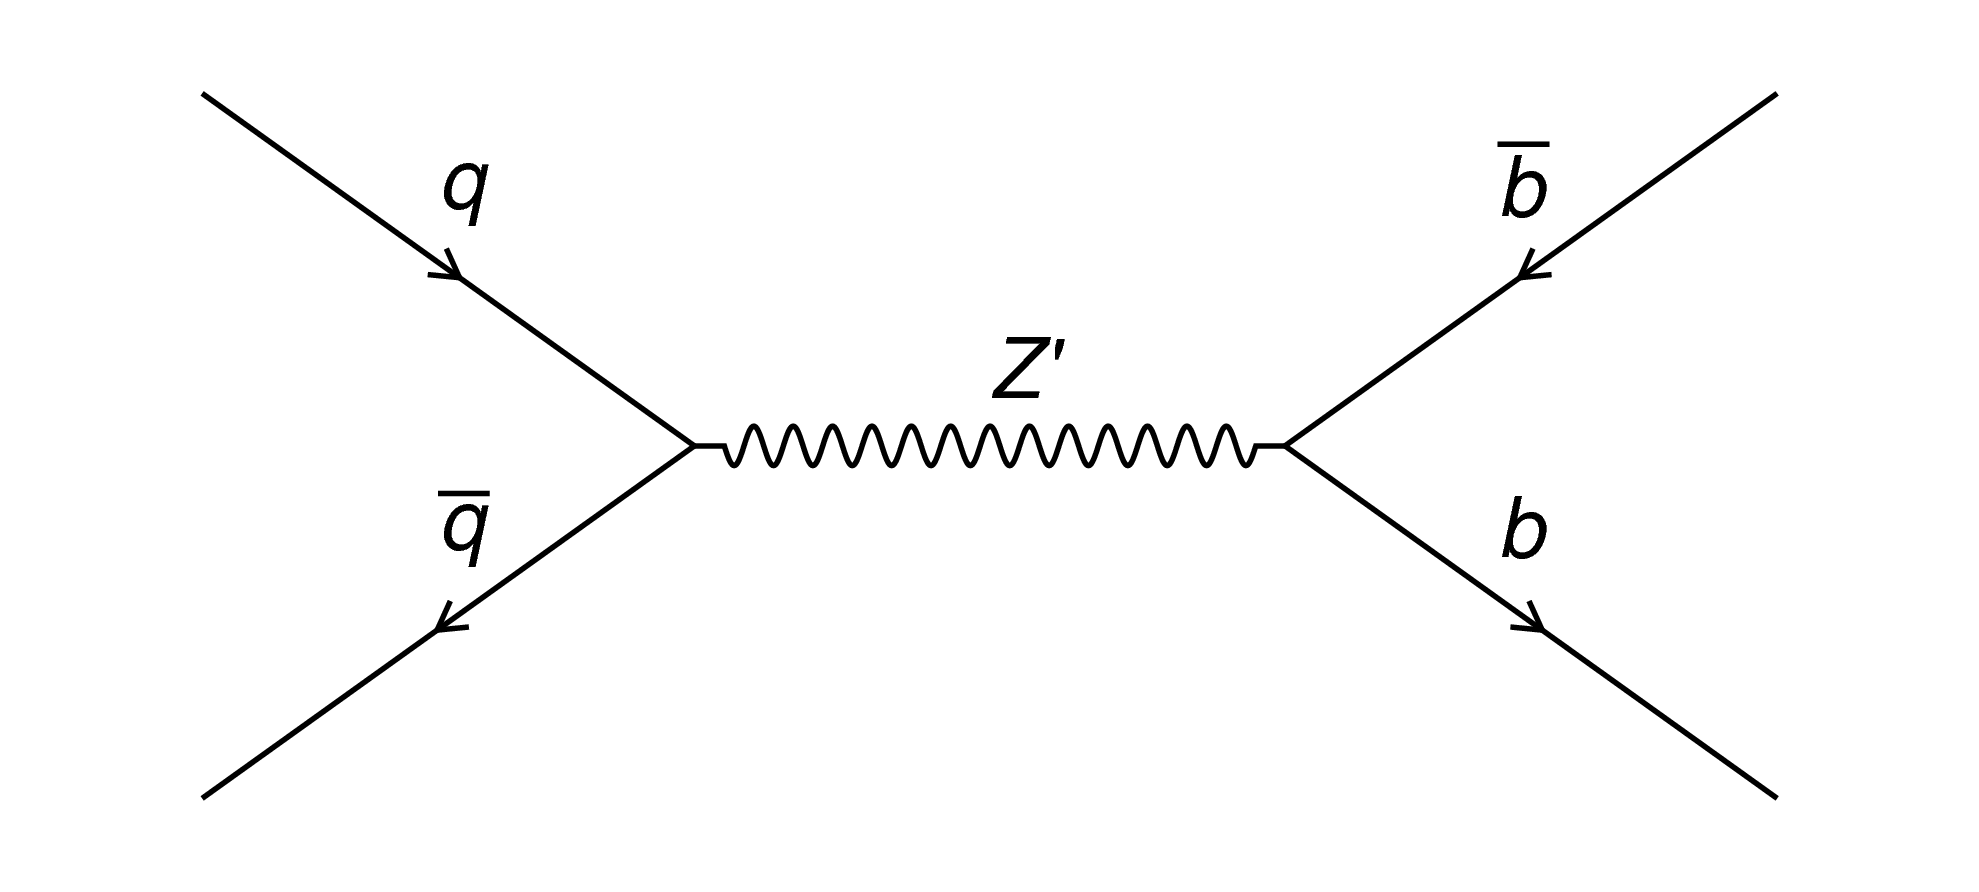
\includegraphics[width=0.7\linewidth, angle=0]{figs/Theory/bsm_zprime.png}
  \end{center}
  \caption{The leading-order Feynman diagram of the process $q\bar{q} \to Z' \to b\bar{b}$.}
  \label{fig:theo-bsm_zprime}
\end{figure}

Three different $Z'$ boson models are considered.
The first is known as the \textit{`Sequential Standard Model'} (SSM) $Z'$ in which the couplings
of the new $Z'$ boson are the same as the Standard Model.
The strongest limits on the SSM $Z'$ boson at the TeV scale are set by searching for a $Z'$ boson decaying
to lepton pairs~\cite{theo-bsm_dilep} \footnote{Because a di-lepton signature is distinct to the large QCD dijet backgrounds produced in $pp$ collisions}.
The second model is a \textit{`leptophobic'} $Z'$ boson that does couple to the lepton sector
but has the same coupling to each of the quarks as the Standard Model~\cite{theo-bsm_zprime_leptophobic},
this model is therefore not strongly constrained by di-lepton searches.

The final model is a \textit{`Dark Matter inspired'} (DM) $Z'$ model;
in which the DM $Z'$ boson acts as a Dark Matter mediator which can couple to both the Dark Matter sector and the Standard Model quark sector~\cite{theo_bsm-zprime_dm}.
The motivation for a Dark Matter mediator was discussed in Section~\ref{sec:theo_bsm_dm}.
This model introduces an additional $U(1)'$ symmetry and a Dirac fermion Dark Matter particle that only interacts through the new gauge group.
The resulting DM $Z'$ boson does not couple with the lepton sector
and couples with the DM fermion and the Standard Model quark sector with couplings $g_\chi$\hspace{0.1mm} and $g_{SM}$\hspace{0.1mm}, respectively.

It is worth noting in the models considered the $Z'$ boson does not preferentially decay to $b$-quarks but rather with similar branching ratio as the other quarks.
However, this can still be considered as preferential decay to $b$-quarks with respect to the dijet background,
which is dominated by gluons and quarks from the first two generations, as discussed in Section~\ref{sec:theo-qcd_dijet}.
Furthermore, there exists $Z'$ models that do not couple to all generations equally~\cite{theo-bsm_zprime_3g},
such that a $Z'$ boson preferentially decaying to $b$-quarks is possible.
%For example; attempts to merge the electro-weak and strong interactions in a so-called 'Grand Unified Theory'
%often use higher symmetries, such as $SU(5)$ or $SO(10)$.

\subsubsection{Excited Third-Generation Quark}
\label{sec:theo-bsm_bstar}

To explain the generational and mass structure of the quark sector, discussed in Section~\ref{sec:theo-bsm_3g},
quark compositeness models describe quarks, not as fundamental particles, but instead constructed of other fundamental particles.
One consequence of quark compositeness models is the prediction of excited quarks, $q^{*}$, which can be observed as heavy resonances.

In particular we consider an excited 3rd generation quark, the $b^{*}$ quark.
The dominant decay mode of a $b^{*}$ quark is to $bg$ with a branching ratio of 85\%
while the remaining decay modes are to $Wt$, $bZ$ and $b\gamma$ with branching ratios of 10\%, 4.5\% and 0.5\% respectively
\footnote{Using the assumptions outlined in~\cite{theo-bsm_bstar}.}.
A Feynman diagram showing the  dominant production and decay mode of a $b^*$ quark is shown in Figure~\ref{fig:theo-bsm_bstar}.

\begin{figure}[!hbt]
  \begin{center}
    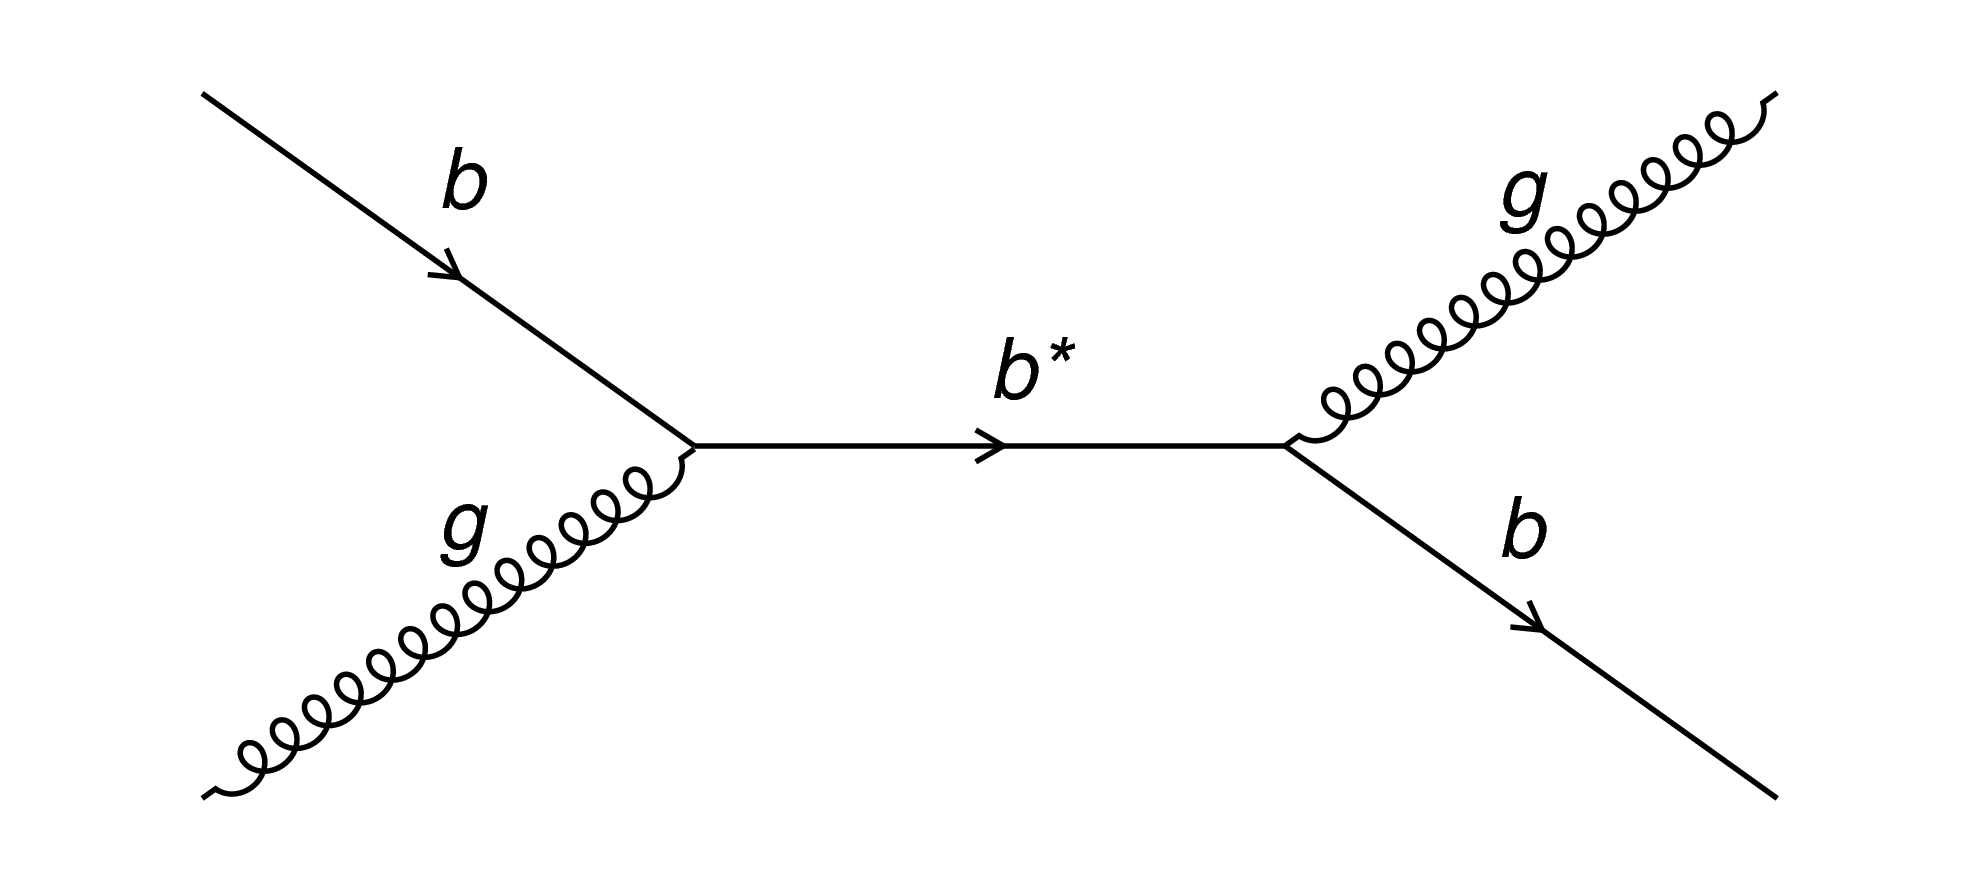
\includegraphics[width=0.7\linewidth, angle=0]{figs/Theory/bsm_bstar.png}
  \end{center}
  \caption{The leading-order Feynman diagram of the process $bg \to b^* \to bg$}
  %\caption{A Feynman diagram showing the dominant production and decay mode of a $b^{*}$ quark.}
  \label{fig:theo-bsm_bstar}
\end{figure}


\subsubsection{Model Independence}

The two benchmark models demonstrate that searching for particles decaying to one or two $b$-quarks is well motivated.
However, it is important to note that the prior belief in any specific model of BSM is small.
This is because there are many BSM theories proposed and there is little evidence to prefer one model over another.
In addition, one must also consider that the true theory may not have been anticipated, such that experiments might be able to see evidence of something truly unexpected.

%Therefore, one should construct searches for BSM to be as model independent as possible,
%rather than optimising specifically for any one model in particular.

This means that the di-$b$-jet searches should be constructed to be
sensitive to as many BSM models as possible
and allow for the unexpected gifts that nature might throw up.

\chapter{The ATLAS Detector}
\label{sec:det}

\section{The Large Hadron Collider}
\label{sec:det-LHC}

High-energy particle colliders have been an essential tool in high-energy physics research for over 50 years,
with a rich history of discovering new particles as each generation of collider pushes the energy frontier;
including the discovery of the Z and W bosons using the Super Proton Synchotron at CERN in 1983~\cite{det-Wdisc_UA1, det-Zdisc_UA1, det-Wdisc_UA2, det-Zdisc_UA2} 
and the discovery of the  top-quark at the Tevatron in 1995~\cite{det-tdisc_CDF, det-tdisc_D0}.

The Large Hadron Collider (LHC) is the highest energy collider ever built,
operated by the \textit{Conseil Europ\'een pour la Recherche Nucl\'eaire (CERN)}.
Lying in a tunnel \SI{100}{\metre} beneath the Swiss/French border near Geneva,
the LHC is a \SI{27}{\km} circumference ring of superconducting magnets and accelerating structures,
which accelerate beams of protons to a maximum energy of \SI{6.5}{\TeV}.
These proton beams are collided in four different locations on the LHC ring
and around each collision point a different detector is constructed to observe these collisions;
one such of these detectors is ATLAS.

\subsection{LHC running conditions in 2015 and 2016}

Since May 2015 the LHC has been colliding bunches of protons at a center-of-mass energy of \SI{13}{\TeV},
the highest energy collisions ever obtained by a particle collider
\footnote{The period of data-taking from 2015 is known as Run-2.}.
In 2015 and 2016 the LHC produced pp collisions 
with a bunch spacing of \SI{25}{\nano\second}\footnote{A small amount of data in 2015 was collected with a bunch spacing of \SI{50}{\nano\second}}
and an average number of collisions per bunch-crossing ($<\mu>$) of 23.7.
%and a maximum peak instantaneous luminosity of \SI{13.8e33}{\cm^{2}\second^{-1}}.
Figure \ref{fig:det-lumi_2015_2016} shows the total luminosity
delivered by the LHC and recorded by ATLAS against date in 2015 and 2016,
showing that a luminosity of \SI{39.5}{\fb^{-1}} was recorded by ATLAS in 2015 and 2016 combined \cite{det-ATLAS_lumi_twiki}.

\begin{figure}[!ht]
  \begin{center}
    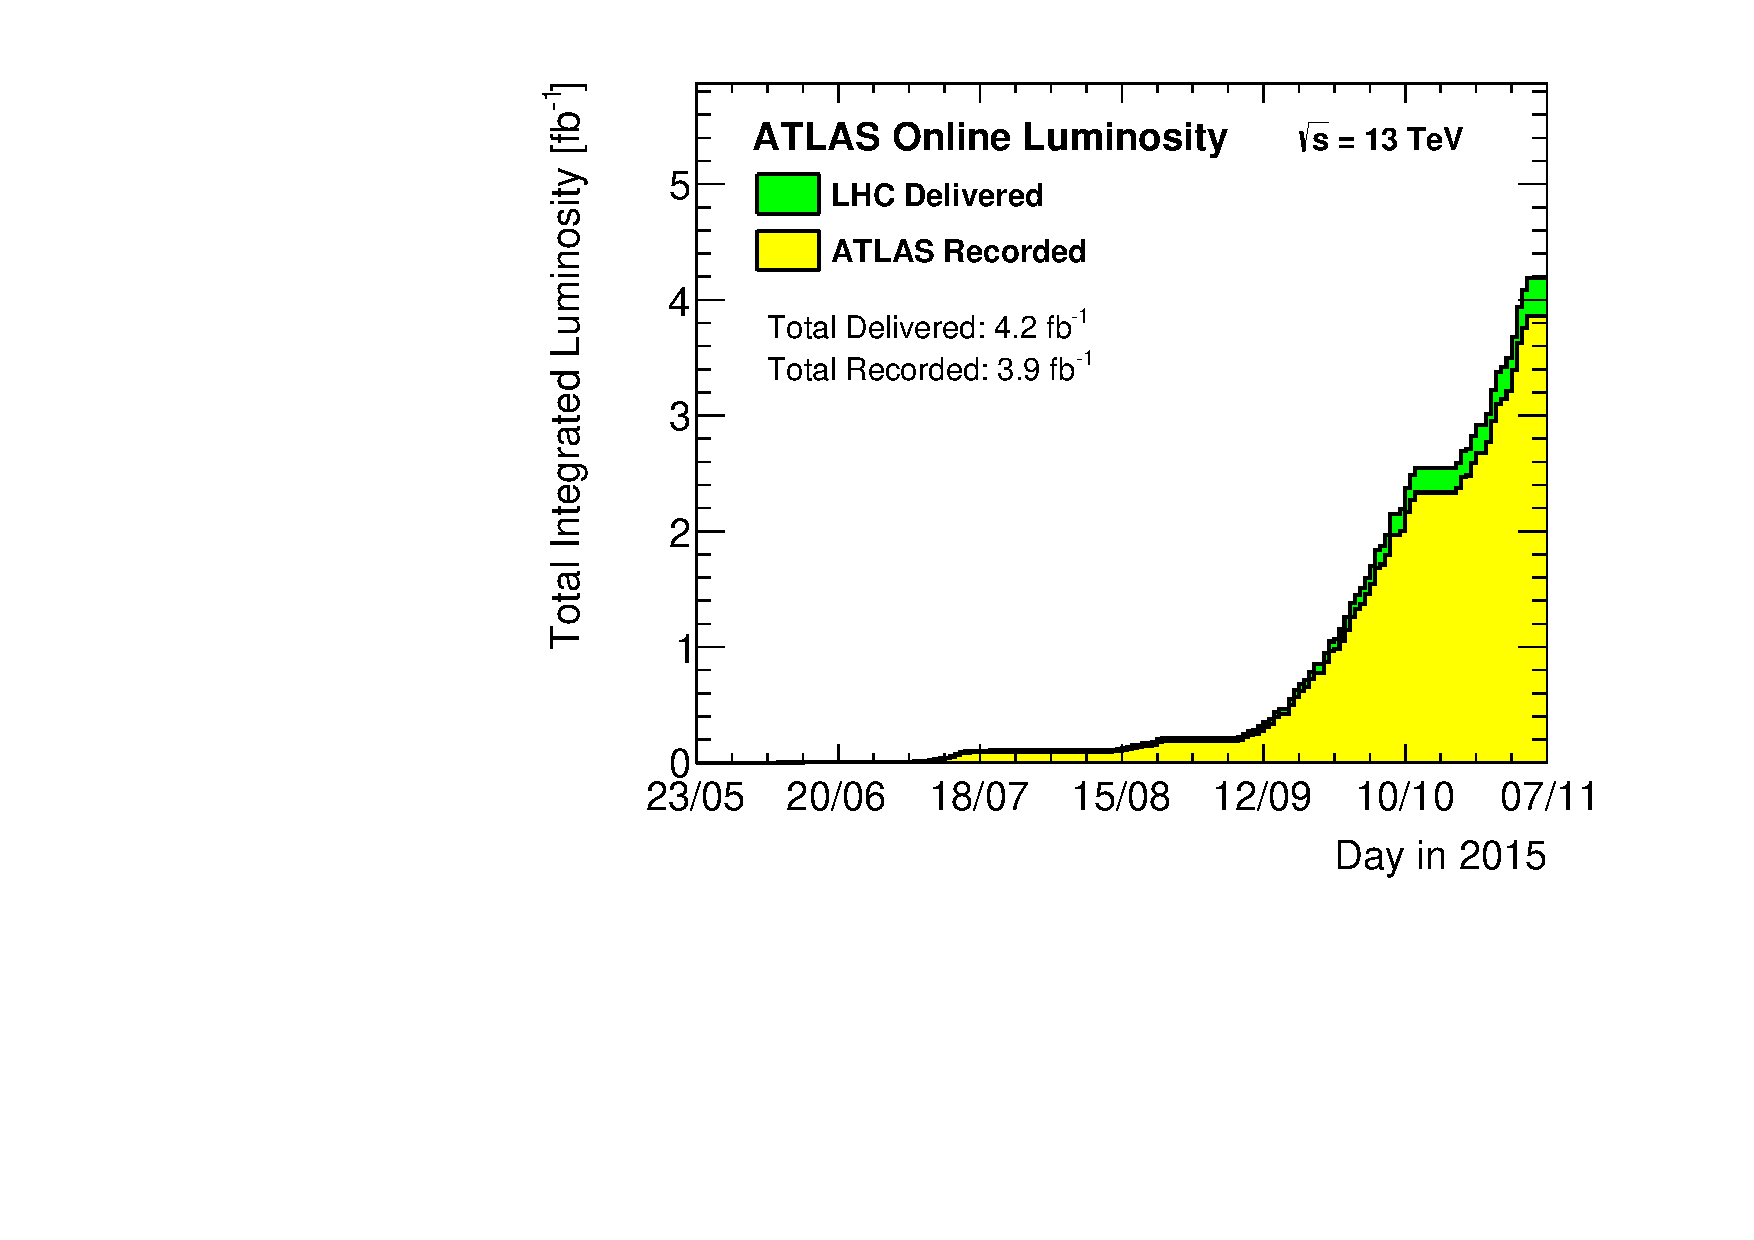
\includegraphics[width=0.45\linewidth, angle=0]{figs/Detector/lumi_2015.pdf}
    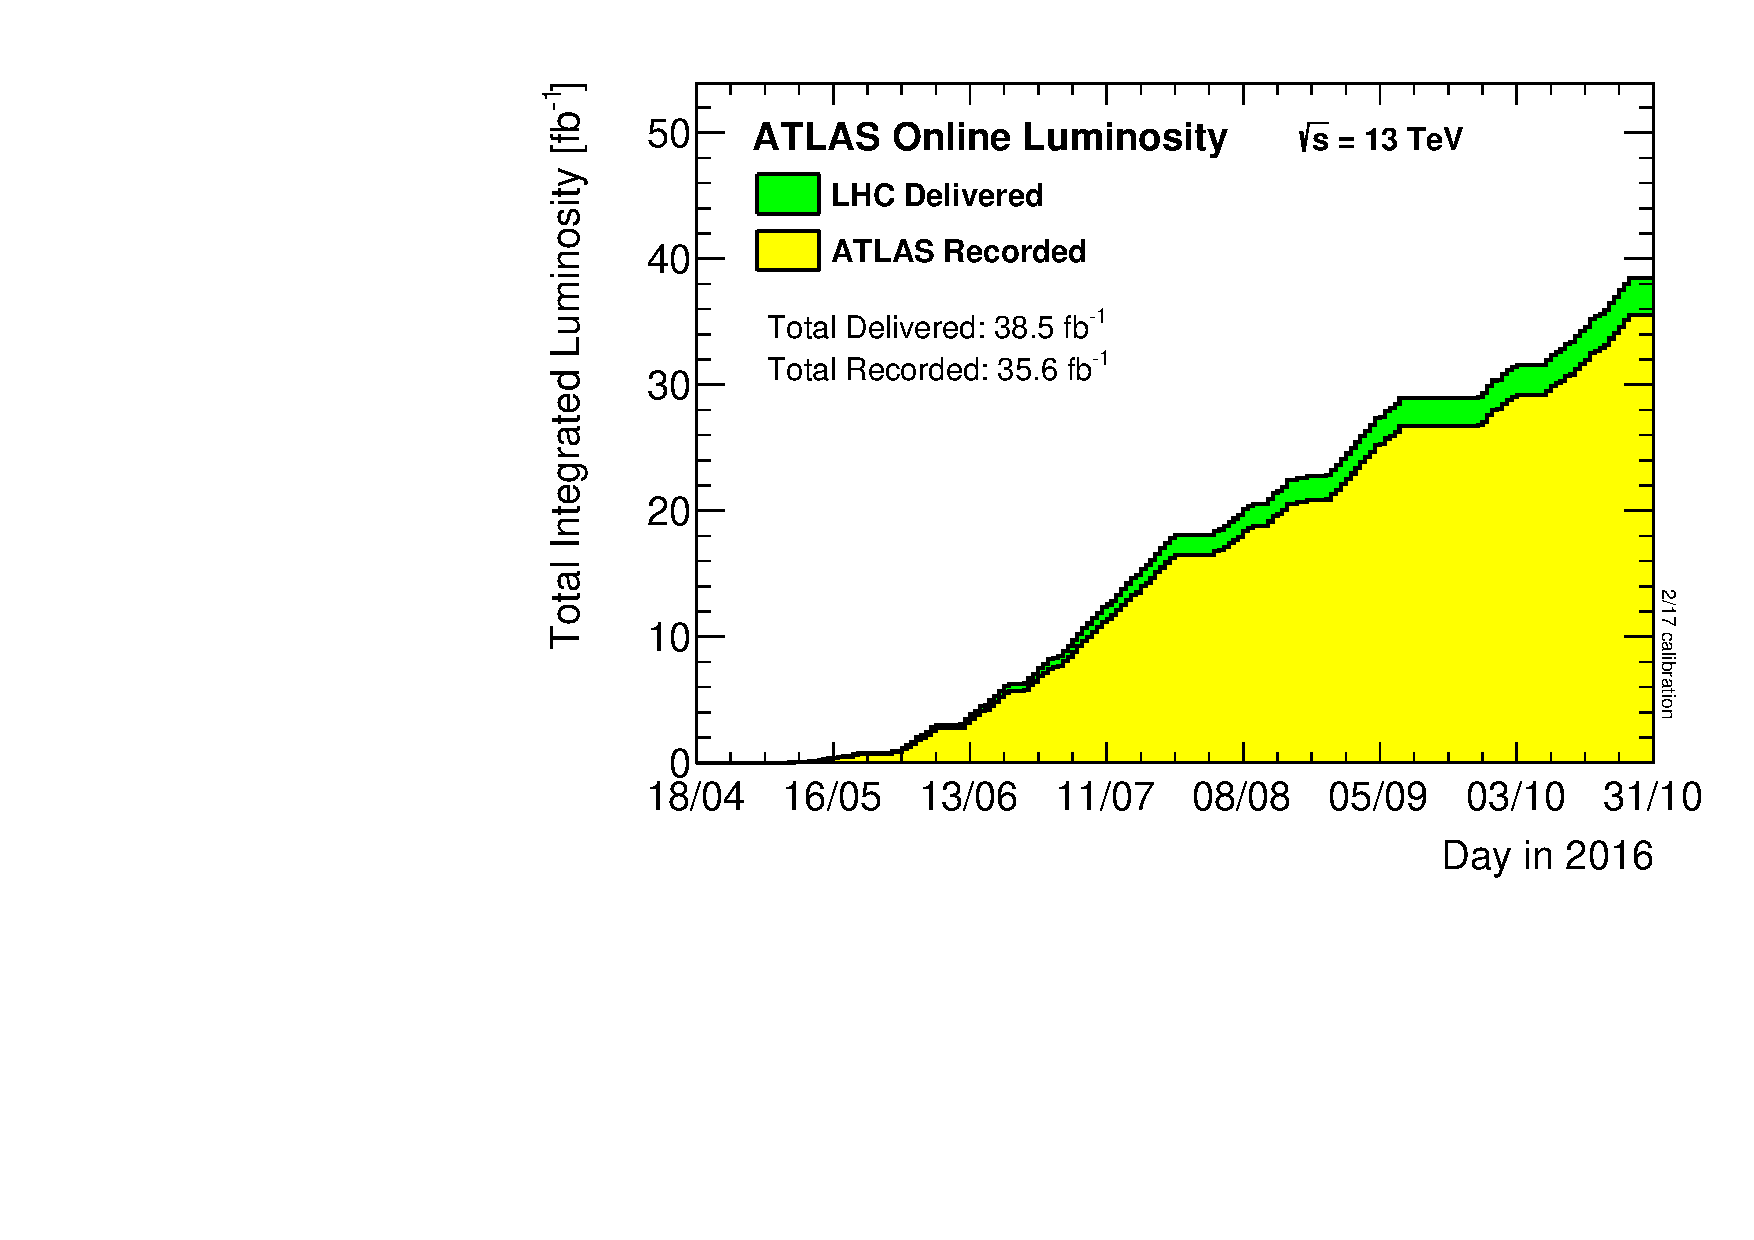
\includegraphics[width=0.45\linewidth, angle=0]{figs/Detector/lumi_2016.pdf}
  \end{center}
  \caption[Cumulative luminosity versus time delivered to (green) and recorded by ATLAS (yellow) during stable beams for pp collisions at 13 TeV centre-of-mass energy in (a) 2015 and (b) 2016]
      {Cumulative luminosity versus time delivered to (green) and recorded by ATLAS (yellow) during stable beams for pp collisions at 13 TeV centre-of-mass energy in (a) 2015 and (b) 2016~\cite{det-ATLAS_lumi_twiki}.}
  \label{fig:det-lumi_2015_2016}
\end{figure}

\section{ATLAS Detector Description}
\label{sec:det-ATLAS}

The ATLAS (\textbf{A} \textbf{T}oroidal \textbf{L}arge Hadron Collider \textbf{A}pparatu\textbf{S}) detector
design, construction and performance has been described in detail previously
\cite{det-ATLAS_Exp, det-ATLAS_TDR, det-ATLAS_Perf},
so what follows in this chapter is a general description of the detector with a focus on the
needs of the analysis that is being presented.
The ATLAS detector is effectively a large closed cylindrical detector,
made up of four key components which sit in concentric rings around the interaction point, where the proton bunches collide.
These components are the inner detector, calorimeters, muon spectrometer and the magnets; each of which are described in further detail below.
This design is used as each sub-detector measures different quantities and interacts differently to the various range of particles that ATLAS is required to observe,
meaning the ATLAS detector is able to identify and measure the key properties of particles that pass through its volume.
Figure~\ref{fig:det-ATLAS_schem} shows a cut-away schematic of the detector
and Figure~\ref{fig:det-ATLAS_slice} shows a slice of the detector in the plane perpendicular to the beam-pipe,
overlaid are simplified illustrations how the detector can respond to a range of particles~\cite{det-thesis_gutchow}.


\begin{figure}[!ht]
  \begin{center}
    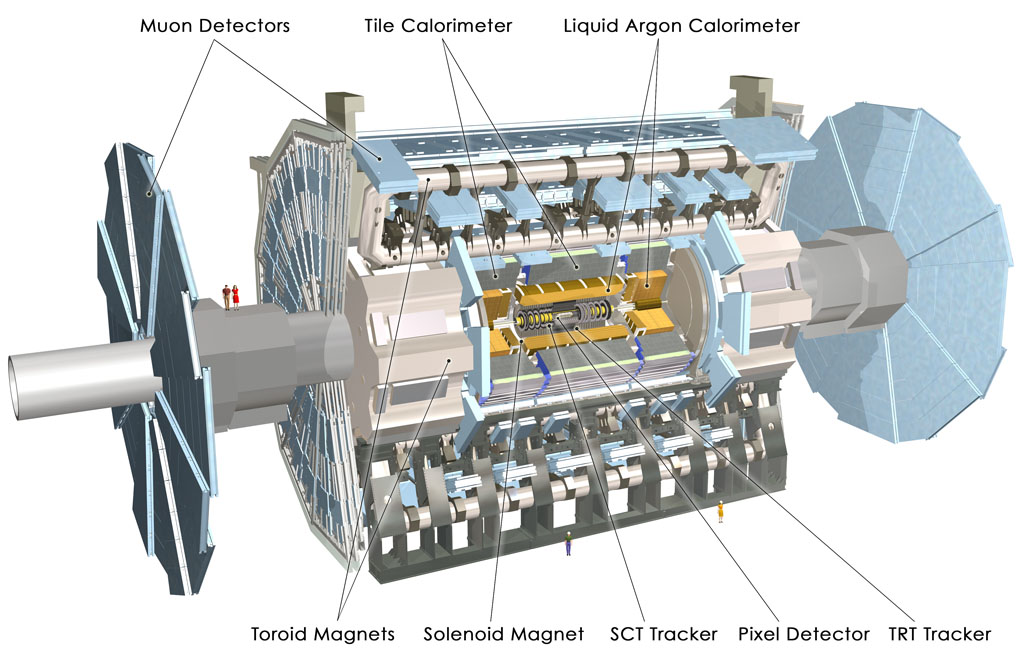
\includegraphics[width=1\linewidth, angle=0]{figs/Detector/ATLAS_schem.jpg}
  \end{center}
  \caption[A cut-away schematic of the ATLAS detector.]{ A cut-away schematic of the ATLAS detector~\cite{det-ATLAS_Exp}.}
  \label{fig:det-ATLAS_schem}
\end{figure}

\begin{figure}[!ht]
  \begin{center}
    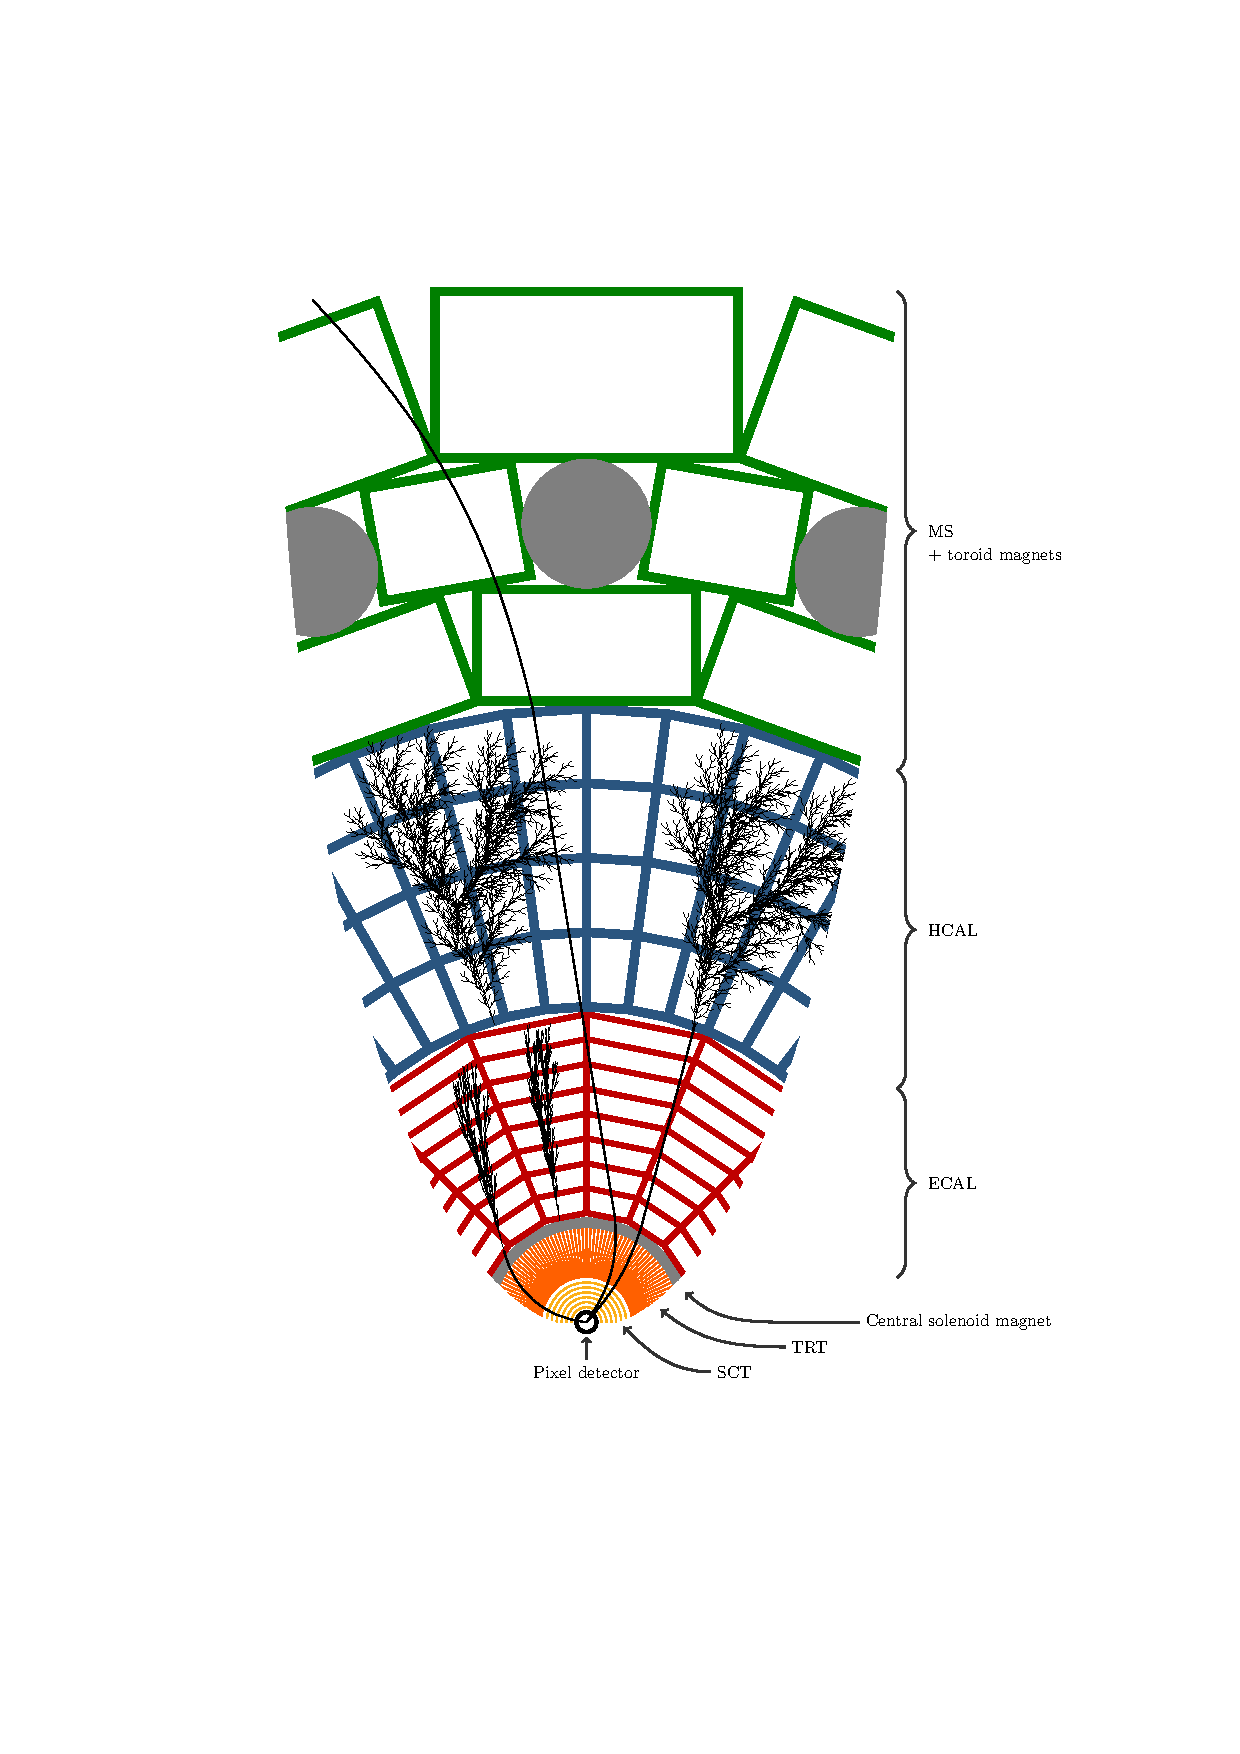
\includegraphics[width=1\linewidth, angle=0]{figs/Detector/ATLAS_slice.pdf}
  \end{center}
  %When citing in a caption, use this set-up
  \caption[A visualisation of the ATLAS detector and the various sub-detectors.
    The view is taken as a slice in a plane perpendicular to the beam-pipe,
    showing the radial range from the beam-pipe to the edge of the detector.
    Overlaid are simplified illustrations of how various types of particles interact with the ATLAS detector;
    specifically from left to right the particles are an electron, a chargeless hadron (e.g. a neutron), a photon, a muon and a charged hadron (e.g. proton).
    The sub-detector components are not to scale.]
          {A visualisation of the ATLAS detector and the various sub-detectors.
    The view is taken as a slice in a plane perpendicular to the beam-pipe,
    showing the radial range from the beam-pipe to the edge of the detector.
    Overlaid are simplified illustrations of how various types of particles interact with the ATLAS detector;
    specifically from left to right the particles are an electron, a chargeless hadron (e.g. a neutron), a photon, a muon and a charged hadron (e.g. proton).
    The sub-detector components are not to scale~\cite{det-thesis_gutchow}.}
  \label{fig:det-ATLAS_slice}
\end{figure}

\subsection{ATLAS Co-ordinate System}
\label{sec:det-coordinate}

Firstly, to describe the detail of the ATLAS detector there must be a description of the co-ordinate system that is used.
ATLAS uses a right-handed coordinate system, in which the origin lies at the interaction point.
The $x$-axis points to the centre of the LHC ring parallel to the surface of the earth,
the $y$-axis points towards the surface of the earth
and the $z$-axis runs along the beam-pipe, pointing anti-clockwise along the LHC beam-pipe.
The azimuthal angle, $\phi$, is defined right-handedly around the $z$-axis starting at the $x$-axis.
%Figure~\ref{fig:det_coordinate} illustrates this co-ordinate system.


The polar angle, $\theta$, is defined as the angle measured from the $z$-axis,
such that along the $z$-axis corresponds to $\theta = 0$
and anti-aligned with the $z$-axis corresponds to $\theta = \pi$.
However, to define the angular direction with respect to the z-axis the ATLAS co-ordinate system uses pseudo-rapidity, $\eta$, instead of using \theta, for reasons that will be outlined below.
$\eta$ is defined as a function of $\theta$:
\begin{equation}
 \eta = -\ln\left[\tan\left( \frac{\theta}{2} \right) \right]
\end{equation}
Thus, $\eta = 0$ corresponds to a particle travelling perpendicular to the beam-pipe,
where a positive value of $\eta$ corresponds to a particle travelling with a tilt towards the $z$-axis.
The quantity is called pseudo-rapidity as in the massless limit ($\lim_{E\to|\vec{p}|}$)
it can be shown that $\eta$ converges to rapidity, $y$, where rapidity is defined as,
\begin{equation}
  y = \frac{1}{2} \ln \left( \frac{E+p_{z}}{E-p_{z}} \right)
\end{equation}
A key property of rapidity is that the differences in rapidity, $\Delta y$, are invariant against Lorentz boosts along the $z$-axis.
Thus, $\eta$ is the final variable chosen in the ATLAS co-ordinate system due to the relation of $\eta$ with both $\theta$ and $y$
and the above mentioned property of $\Delta y$.
One final quantity commonly used within ATLAS is the variable $\Delta R$, which is defined as
\begin{equation}
  \Delta R = \sqrt{\Delta\eta^{2} + \Delta\phi^{2}}
\end{equation}
\Delta R represents an angular separation between two vectors within the ATLAS co-ordinate system.


Now that we have discussed the ATLAS co-ordinate system, we can provide a description of the components of the ATLAS detector.

\subsection{Inner Detector}
\label{sec:det-ID}

The Inner Detector (ID), the innermost sub-detector on ATLAS,
measures the trajectory of charged particles passing through the detector.
The ID is constructed from many concentric layers of detector,
and as a charged particle passes through the detector each of the layers provides a position measurement, known as a hit.
Then using the hits from the many layers the trajectory of the particle can be determined;
the measured trajectory is known as a track.
The ID is immersed in a 2~T magnetic field which bends the particle's trajectories;
from the sign and magnitude of the track's curvature the charge and momentum of the particle can be inferred.
The ID is made of three main component parts; the pixel detector, the Semi-Conductor Tracker
(SCT) and the Transition Radiation Tracker (TRT), as visualised in Figure~\ref{fig:det-ID_schem}.
The ID consists of the barrel, which are made up of cylinders surrounding the beam-pipe to cover low absolute values of $\eta$,
and the end-caps, which lie  perpendicular to beam-pipe on either end of the barrel to cover large values of absolute $\eta$:
here the description focuses on the barrel as this covers the $\eta$ range considered by the analysis.

\begin{figure}[!ht]
  \begin{center}
    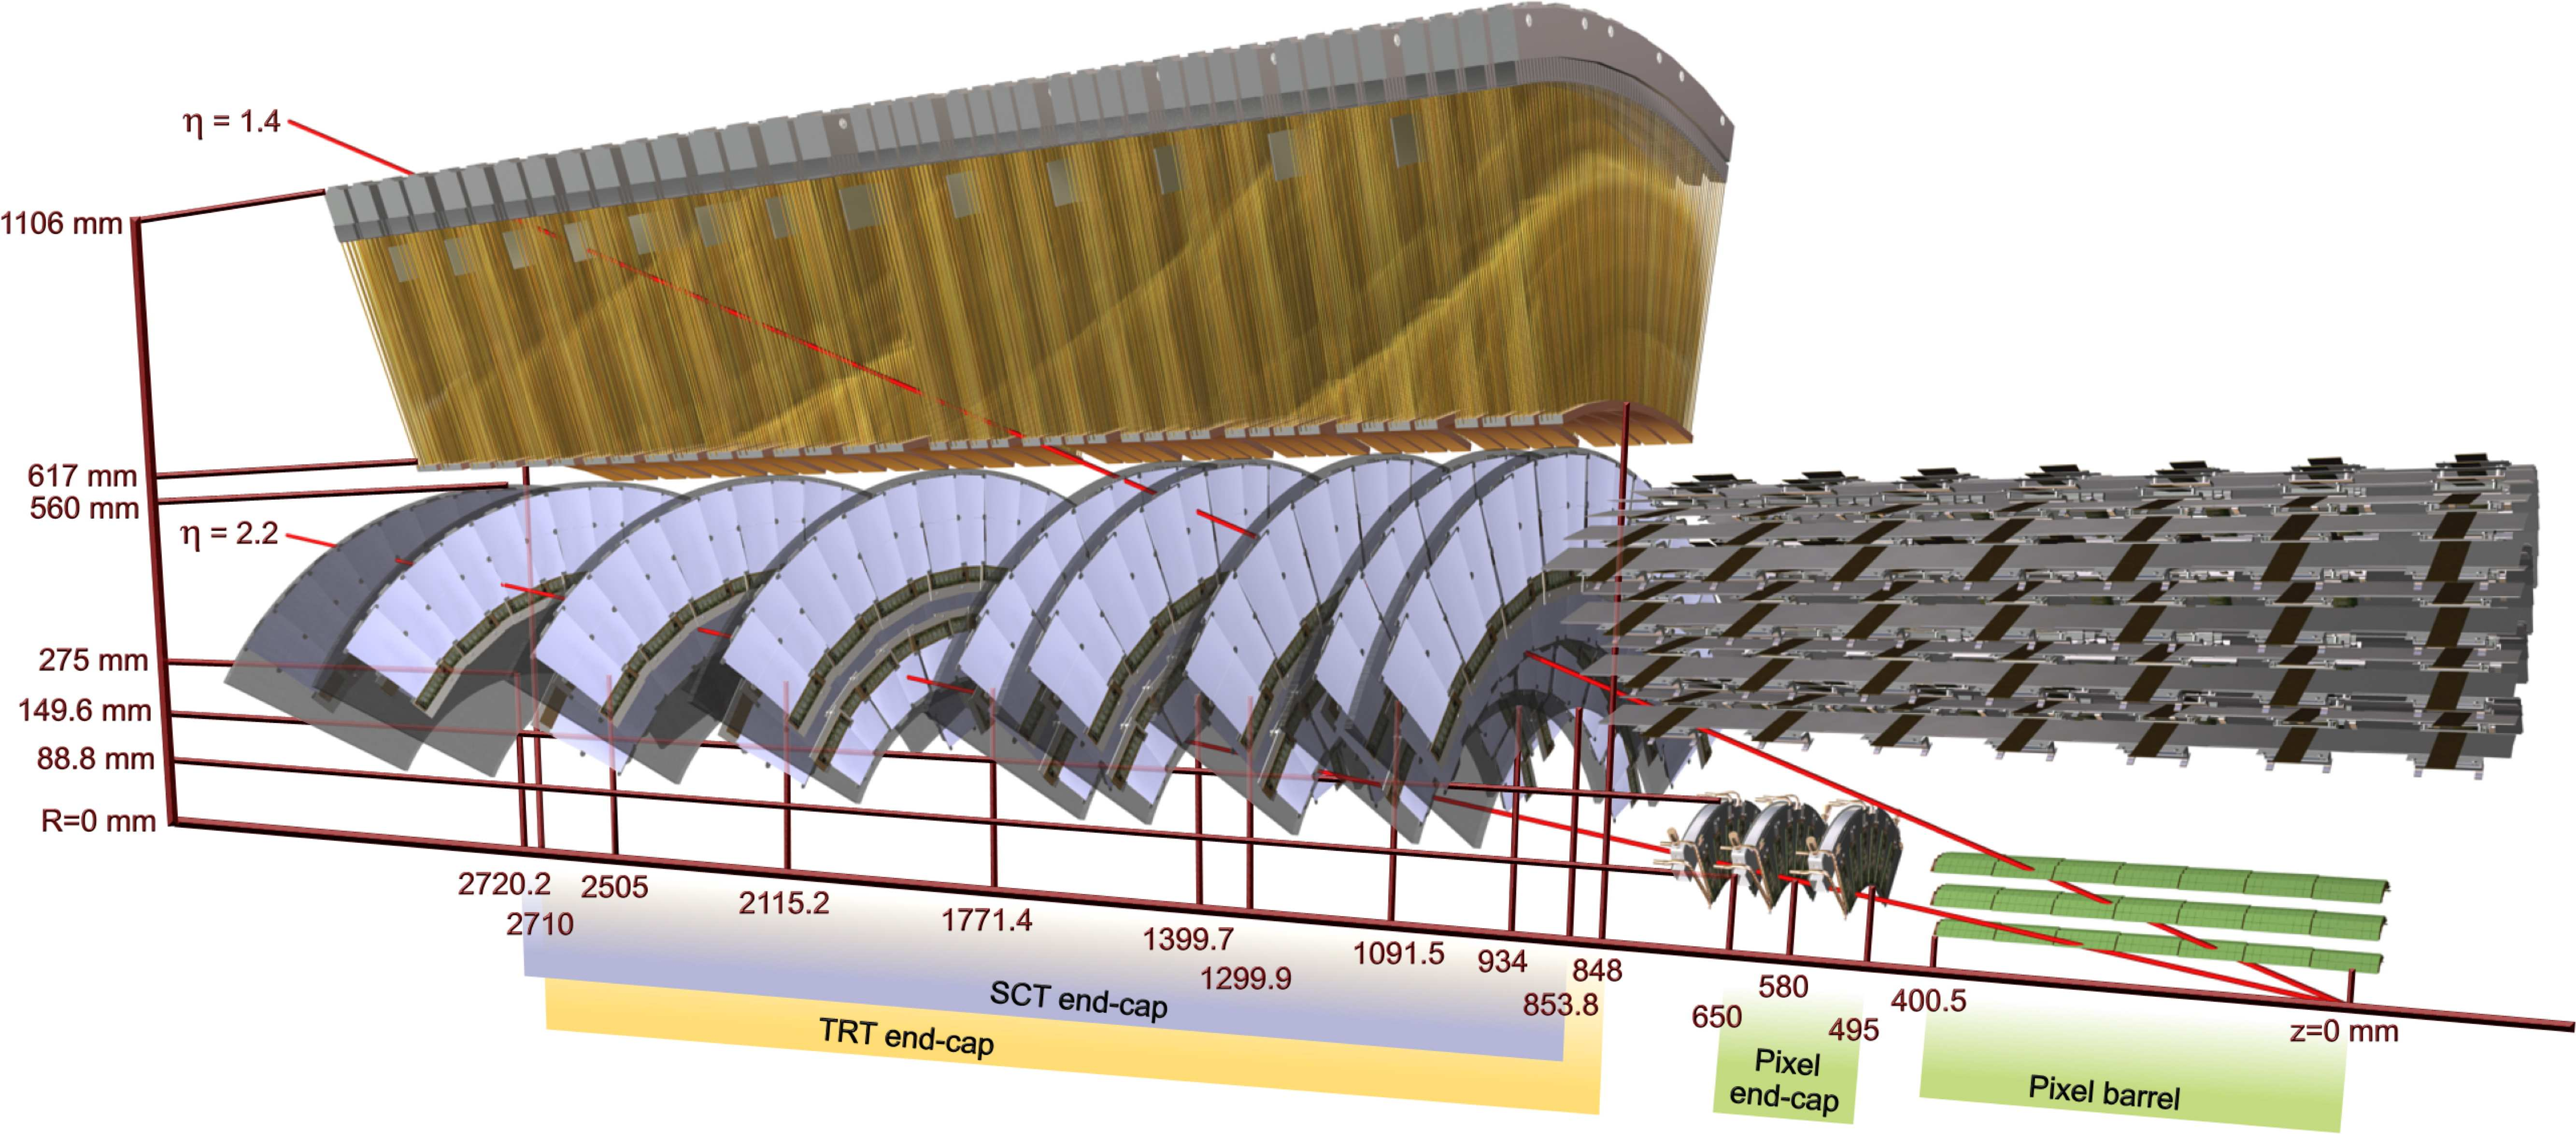
\includegraphics[width=0.8\linewidth, angle=0]{figs/Detector/ID_schem.pdf}
  \end{center}
  \caption[A cut-away schematic of the ATLAS Inner Detector (ID).]{A cut-away schematic of the ATLAS Inner Detector (ID)~\cite{det-ATLAS_Exp}.}
  \label{fig:det-ID_schem}
\end{figure}

The innermost component of the ID is the silicon pixel detector;
in the barrel this detector consists of 4 high-granularity layers of silicon based pixel modules surrounding the beam pipe,
covering a range of $-2.5 < \eta < 2.5$ and a radial distance of \SI{33}{mm} to \SI{122.5}{mm} \cite{det-IBL_TDR, det-IBL_Talk}.
The high-granularity of the pixel layers, allows for high precision measurements,
with an intrinsic resolution of approximately resolution of $\sim$\SI{10}{\micro\metre} in $R-\phi$ plane
and $\sim$\SI{115}{\micro\metre} in the z-direction. 

Moving radial outwards the next component of the ID is the Semi-Conductor Tracker;
which, in the barrel, comprises of 4 cylindrical layers of silicon micro-strips
covering a range of $-2.5 < \eta < 2.5$ and a radial distance of 299 mm to 514 mm.
The SCT has an intrinsic resolution of $\sim$\SI{17}{\micro\metre} in $R-\phi$ plane
and $\sim$\SI{580}{\micro\metre} in the z-direction. 

The outermost component of the ID is the Transition Radiation Tracker (TRT)
constructed of many \SI{4}{\mm} radius tubes filled with xenon.
As a charged particle passes through the gas,
it will cause ionisation allowing a measurement of its position using drift-time.
In the barrel, each tube provides a measurement in the $R-\phi$ plane
with an intrinsic resolution of ~\SI{130}{\micro\metre}
and the TRT will typically provide 36 hits per track.
In addition to a position measurement, due to the choice of the material between the tubes,
a particle passing through the detector will radiate photons
at an intensity inversely correlated to the mass of that particle,
providing additional information for particle identification. 

The trajectory, momentum and charge measurements provided by the Inner Detector are essential for particle identification in ATLAS.
In particular, the high precision measurements close to the beam-line allow for vertex reconstruction,
which is essential for identification of tracks coming from B or C hadrons, and hence the identification of $b$-jets.
This process, known as $b$-tagging, is discussed further in Section~\ref{sec:obj-bjets}\textit{(object definition and selection)}
and is important within the context of this analysis. 

\subsection{Calorimeters}
\label{sec:det-calo}

The ATLAS calorimeter, located on the outside of the magnet solenoid surrounding the ID,
is designed to provide an energy measurement of the traversing particles.
Accurate energy measurements are essential for a good resolution
of the mediator mass reconstructed from its decay products,
which is important within the context of the analysis being presented in this thesis.

The calorimeter at ATLAS is made up of two different systems that are built in concentric rings;
the inner-most is the Electromagnetic Calorimeter system (ECAL), which is used to measure electromagnetic objects such as photons and electrons.
Outside of that is the Hadronic Calorimeter system (HCAL), designed to provide an energy measurement of hadronic material.
The HCAL is built from the Tile and Hadronic Endcap calorimeters.
Both the ECAL and HCAL have barrel and end-cap components to make energy measurements at a large range of $\eta$ values.
Figure \ref{fig:det-calo_schem} shows a cut-away of the ATLAS calorimeter.

\begin{figure}[!ht]
  \begin{center}
    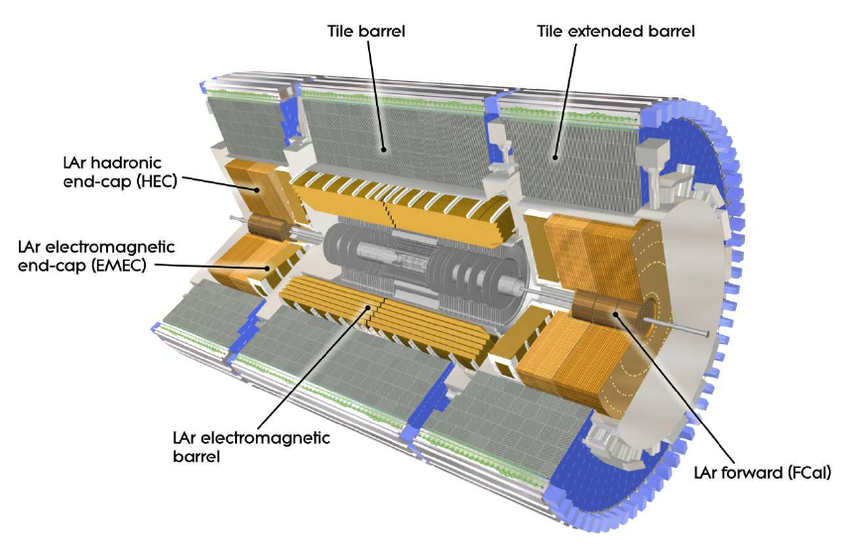
\includegraphics[width=1\linewidth, angle=0]{figs/Detector/Calo_schem.png}
  \end{center}
  \caption[A cut-away schematic of the ATLAS calorimeter system.]
          {A cut-away schematic of the ATLAS calorimeter system~\cite{det-ATLAS_Exp}.}
  \label{fig:det-calo_schem}
\end{figure}

Below I provide a more detailed description of the calorimeter components;
however, the principle behind each detector is common so is described first.
The calorimeters at ATLAS are sampling calorimeters, which means they consist of alternating layers of absorber and active material.
The role of the of the absorber layer is to force the particle, whose energy we want to measure, to emit secondary particles.
These secondary particles will again emit further particles and so on meaning a ``particle cascade'' is formed.
The role of the active material layer is to measure the energy of the many resulting particles from the cascade, known as the cascade particles.
The ATLAS detector is built such that the initial particle will cascade within the volume of the calorimeter system
and then, from a measurement of the energy of all the cascade particles,
the energy of the initial particle can be inferred. 

\subsubsection{Electromagnetic Calorimeter (ECAL)}

For the electromagnetic interaction, at energies $\sim \geq$\SI{1}{\GeV} the particle cascade process is mainly caused by two processes;
bremsstrahlung, ($e^{+/-} \to e^{+/-} + \gamma$) and pair production ($\gamma \to e^{+} + e^{-}$).
The electromagnetic calorimeter at ATLAS is known as the Liquid Argon (LAr) calorimeter.
The absorber material used in the LAr calorimeter is lead, due to its large density of charged particles (high Z)
which increases the rate of the cascade processes.
The active material is liquid argon;
when a cascade particle passes through the liquid argon it causes ionisation,
and the released electrons are captured using an electric field.
The number of released electrons is proportional to the energy of the cascade particle,
meaning that the energy of the cascade particle can be measured. 

As discussed above the LAr is split up into two sections;
the barrel section covers a region of $|\eta| < 1.475$ and two end-cap components cover $1.375 < |\eta| < 3.2$.
The depth of an electromagnetic calorimeter is often expressed in terms of the radiation length, $X_{0}$,
which is the distance that an electron's energy reduces by a factor of $e^{-1}$ through bremsstrahlung,
or 7/9 of the mean free path for a photon to pair produce electrons.
It is worth noting that this quantity is strongly material dependant;
a high-Z material, such as lead, has a shorter $X_0$.
The LAr calorimeter has a depth of $>$ 22 $X_{0}$ in the barrel and $>$ 24 $X_{0}$ in the end-caps,
meaning that almost all of the particle shower from a high-energy photon
or electron can be contained within electromagnetic calorimeter. 

\subsubsection{Hadronic Calorimeter (HCAL)}
\label{sec:det-calo_HCAL}

If a particle can also interact through strong interactions, such as the components of a hadronic jet,
then the particle cascade is a more complicated process.
A hadronic cascade processes is dominated by processes such as
ionisation, nuclear spallation and neutron generation \cite{det-nuclearInt_book, det-thesis_kate}.
For a chargeless hadron, for example a neutron,
strong processes, such as spallation, are the only processes that contribute to its cascade.
During these hadronic cascade processes many $\pi_0$ mesons are made,
which can decay to a pair of photons and thus form electromagnetic cascade as described above. 

For hadronic interactions, the size of detector is measured by the interaction length, $\lambda$,
defined as the distance required to reduce the number of relativistic hadrons by $e^{-1}$.
This means that by the end of the LAr calorimeter there is 2.3 $\lambda$ of active material in the barrel,
so the full hadronic shower cannot be captured by the LAr calorimeter alone.
For a full measurement of the hadronic energy, the Hadronic Calorimeter system (HCAL) is required. 

The Tile Calorimeter is constructed from absorber layers of steel and active material layers of scintillating tiles,
and has a depth of 7.4 $\lambda$, meaning the majority of the hadronic shower can be captured by either the LAr calorimeter or the Tile calorimeter.
The Tile Calorimeter is split up into the barrel and the extended barrel components;
the barrel covers the region $|\eta| <$ 1.0 and the extended barrel covers the region $0.8 < |\eta| < 1.7$. 

To cover the more forward regions there are two more calorimeter detectors.
The Hadronic Endcap Calorimeter (HEC) is housed in two large wheels at either end of the ATLAS detector
and covers a region of $1.5 < ∣\eta∣ < 3.2$.
The HEC is a sampling calorimeter built using copper as the absorber layers and liquid argon as the active material
and has a depth of $\sim 12~\lambda$.
In addition the Forward Calorimeter (FCAL) covers the very forward region of $3.1 < ∣\eta∣ < 4.9$,
which is outside the range considered within this analysis.
It is constructed from absorber layers of
copper (for EM interactions)
and tungsten (for hadronic interactions)
with liquid argon for the active material layers. 

Another important point about the ATLAS calorimeter is that it is non-compensating calorimeter;
that is to say that the response of the detector to an electromagnetic particle (such as an electron)
is larger than the response of a hadronic particle (for example a pion).
The reason for this is some energy is lost in hadronic cascade process;
mainly due to the energy required to release nucleons from calorimeter nuclei during spallation,
but also from the recoil energy given to the calorimeter nuclei
and neutrinos created during strong processes that can escape the calorimeter \cite{det-comp_calo, det-thesis_lene}.
To account for the fact that the ATLAS calorimeter is non-compensation,
calorimeters are calibrated to the EM-scale,
which means that the inital energy measurement of a calorimeter assumes that the particle EM-interacting.
Then for a hadronic object a jet energy scale correction is applied in the jet calibration processs,
which is described further in Section~\ref{sec:obj-jet_calib}.

\subsection{Muon Spectrometer}
\label{sec:det-MS}

The only standard model particle visible to ATLAS which can pass through the calorimeter is the muon;
hence to identify and obtain the momentum of muons an additional detector, the Muon Spectrometer (MS), is used.
The MS is a detector which surrounds the hadronic calorimeter,
measuring the momentum of muons by observing the curvature of their trajectories in magnetic fields.
Trajectories are determined using muon position measurements from multiple layers of detectors,
analogous to what has been described for the inner detector. 

In the barrel region ($|\eta| < 1.4$) the large barrel toroid provides the magnetic field,
in the end-cap region ($1.6 < |\eta| < 2.7$) the two smaller end-cap magnets  provide the magnetic field
and finally in the transition region ($1.4 < |\eta| < 1.6$) both sets of magnets contribute to the magnetic field.
A further description of the magnets used in ATLAS is found in the next section. 

Muon chambers are the detectors tasked with providing the muon position measurements required to reconstruct muon tracks.
The muon chambers come in two types; trigger and precision.
The trigger muon chambers provide a quick position measurement in 3-dimensions which can be used
to identify muons tracks in the trigger.
The trigger muon chambers cover a range $|\eta| < 2.0$;
consisting of Resistive Plate Chambers (RPC’s) in the barrel and Thin Gap Chambers (TGC’s) in the end-cap regions.
The precision muon chambers provide a precise measurement of the muon position co-ordinates in the $R-z$ plane,
the plane in which track curvature occurs in the muon spectrometer, allowing for precise measurements of the muon track-$p_T$. 
In the barrel region, precision muon chambers are arranged in three concentric cylindrical layers of chambers formed around the beam-pipe,
whilst in the transition and end-cap regions there are three layers of chambers either side of the barrel lying in disks perpendicular to the beam-pipe.
In the region $|\eta| < 2.0$, the precision muon chambers are made from Monitored Drift Tubes (MDTs),
whilst at large pseudo-rapidities ($2.0 < |\eta| < 2.7$), Cathode Strip Chambers (CSCs) are used.


There is an additional use of the muon spectrometer that relates to high-energy jets.
Whilst for most jets their shower is fully contained within the calorimeter
there are some jets, particularly at high-$p_T$, where a non-negligible fraction of energy from the shower goes beyond the calorimeter.
This effect, known as `punch-through', is accounted for using energy deposits in the muon spectrometer.

\subsection{Magnets}
\label{sec:det-magnets}

\begin{figure}[!ht]
  \begin{center}
    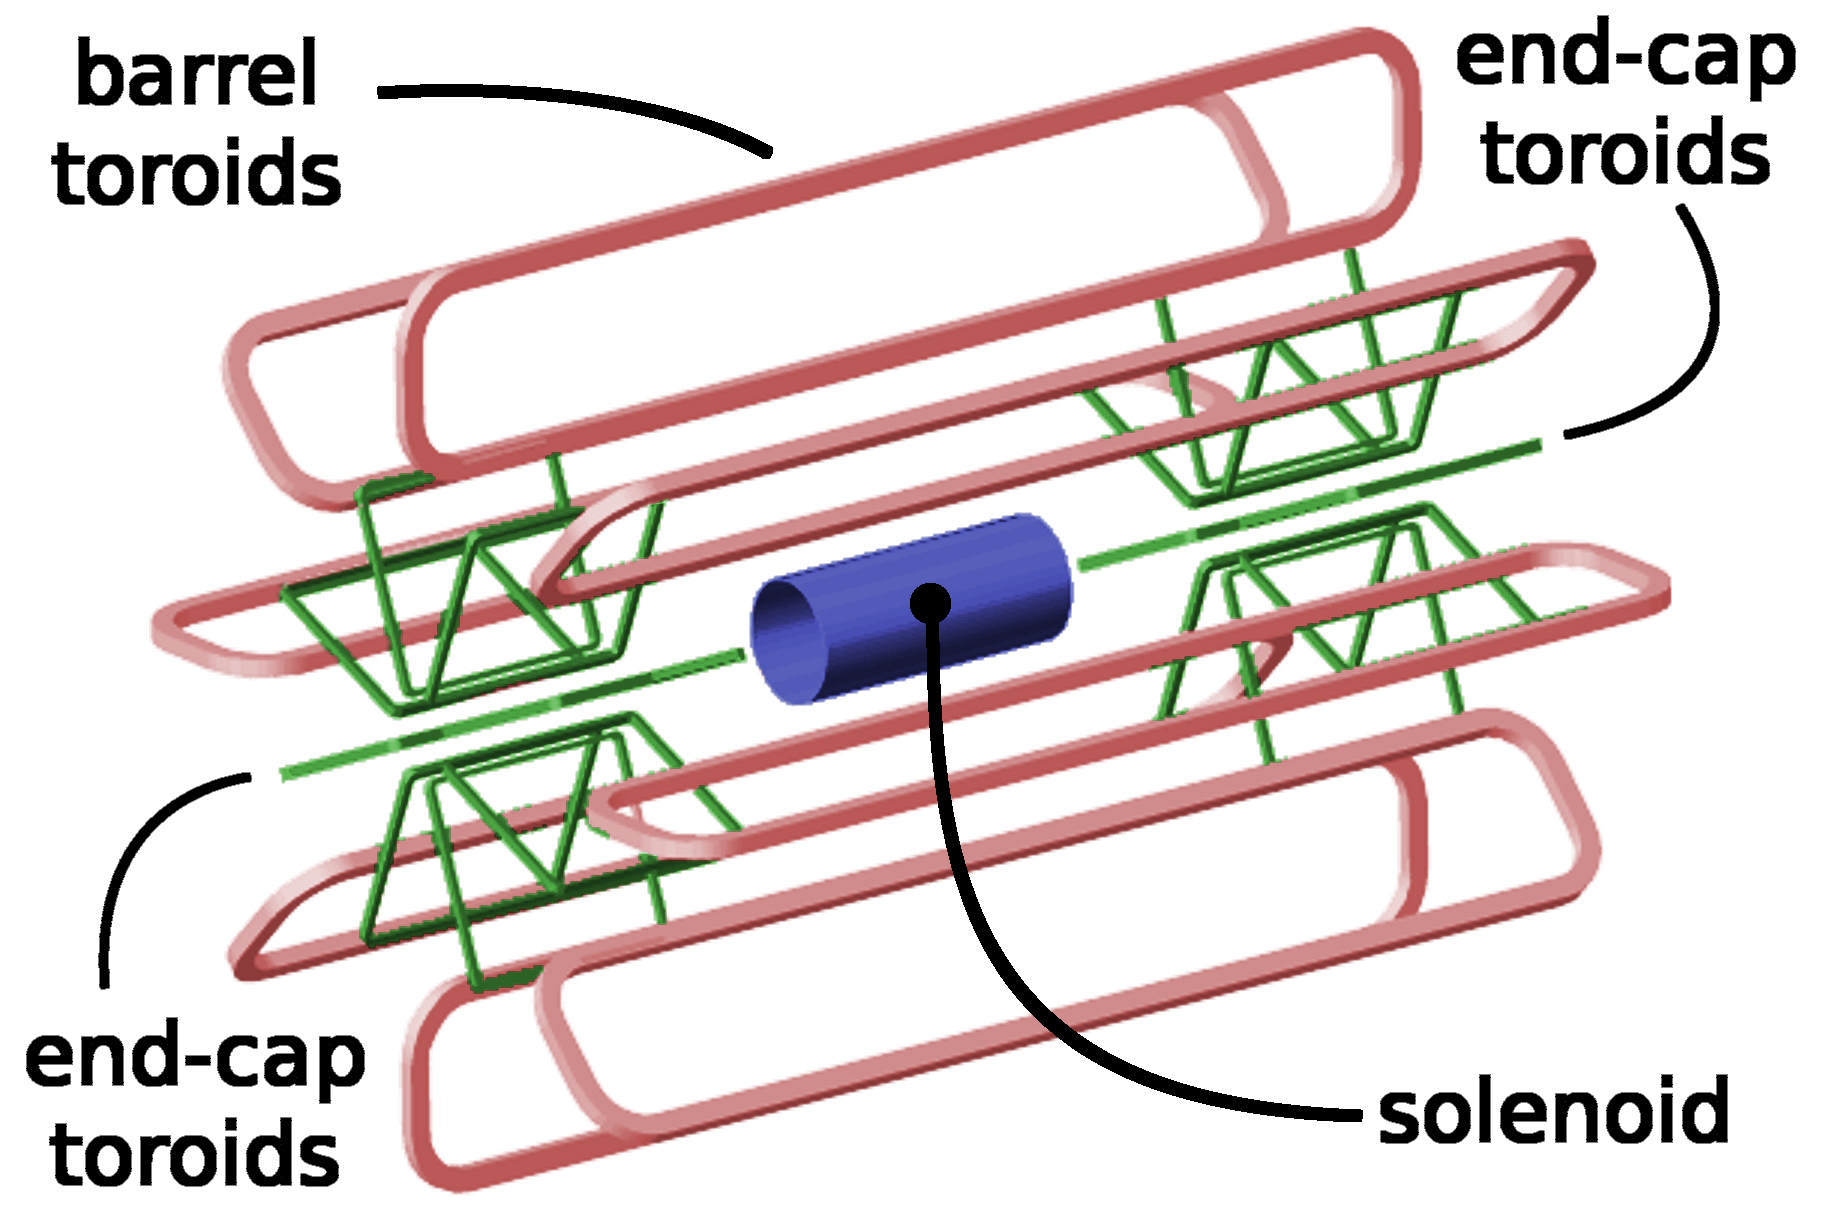
\includegraphics[width=1\linewidth, angle=0]{figs/Detector/Magnet_schem.png}
  \end{center}
  \caption[The layout of the ATLAS magnets.]{The layout of the ATLAS magnets~\cite{det-magnet_fig}.}
  \label{fig:det-magnet_schem}
\end{figure}


In ATLAS magnetic fields are important for obtaining the momentum and charge of particles from their observed trajectories in the ID and Muon Spectrometer.
ATLAS is made up of four large superconducting magnets;
the inner solenoid which surrounds the inner detector and provides a 2~T magnetic field within the ID.
The barrel toroid magnet provides a magnetic field of up to 2.5~T in the central regions of the muon spectrometer and
the two end-cap toroid magnets which produce a magnetic field of up to 3.5~T in the forward regions of the MS.
Figure~\ref{fig:det-magnet_schem} shows the layout of the magnets in ATLAS \cite{det-magnet_fig}.

%\section{Data Acquisition and Trigger}
\section{Trigger}
\label{sec:det-trig}

In 2015 and 2016, the LHC has been colliding proton beams with a spacing of \SI{25}{\nano\second},
meaning that the ATLAS experiment has been taking data at a rate of 40 MHz.
However, due to the large computing resources required to process and store each event,
it is not possible to record all this data for use in an analysis.
To resolve this problem,
the ATLAS experiment uses a trigger system to reduce the event rate by
selecting the events of interest that contain high-$p_{T}$
%$\footnote{$p_{T}$ refers to the component of momentum transverse to the beam-line.} 
physics objects, which indicate that a hard scatter has occurred in that event. 

The ATLAS trigger-system has two levels;
the first level trigger (L1) and the higher level trigger (HLT) \cite{det-run2_trigger}.
Figure~\ref{fig:det-trigger_schem} shows a schematic outlining the trigger used in Run-2 \cite{det-run2_triggerPerf}. 

\begin{figure}[!ht]
  \begin{center}
    \includegraphics[width=1\linewidth, angle=0]{figs/Detector/trigger_schem.png}
  \end{center}
  \caption[A schematic of the ATLAS trigger and data-acquisition system in Run-2, with a focus on the components required for triggering.]
          {A schematic of the ATLAS trigger and data-acquisition system in Run-2, with a focus on the components required for triggering~\cite{det-run2_trigger}.}
  \label{fig:det-trigger_schem}
\end{figure}

The first level trigger (L1) is hardware based which reduces the rate from 40~MHz to 100~kHz within a time window of \SI{2.2}{\micro\second}.
The L1 trigger uses custom electronics to rapidly process information directly from the
calorimeter and the muon spectrometer, searching for high-$p_{T}$ muon tracks and large calorimeter deposits.
The information is then passed to the central trigger which uses a set of pre-defined conditions
to decide if a L1 trigger accept is given and thus events are passed on to the next step of triggering.
At the same time Regions of Interests (ROIs) are constructed around the objects that have fired the L1 trigger,
which are passed on to the HLT. 

The next step is the HLT, a software based trigger,
which further reduces the event rate to 1~kHz within a time window of ~\SI{0.2}{\second}.
The HLT uses the information from the full detector
to perform a more complete reconstruction of the physics objects within the event,
the most time consuming reconstruction algorithms only being run only within the ROIs taken from L1.
The more complex event analysis allowed within the software-based trigger includes
track reconstruction and therefore allows for $b$-jet identification.
If the content of the event reconstruction passes a pre-set criteria, a HLT accept is issued
meaning that the events are passed on for processing and storage. 
% in offline computer farms (known as tier-0). 

A further description of triggers used in the analysis,
with a particular focus on the $b$-jet trigger performance
can be found in \ref{sec:bJetTrigger}\textit{(b-jet trigger chapter)}.


\chapter{Object Definition and Reconstruction}
\label{sec:obj}
\textbf{LM fix} Does citations work here: \cite{trig-evtGen}?


\section{Jets}
\label{sec:obj-jets}
  \subsection{Hadronic cluster reconstruction}
  \subsection{Jet Reconstruction}
   anti-$k_T$
   \subsection{Jet calibration}
    (JES, JER, BJES) description
    
   \section{Identification of $b$-jets}
   \label{sec:obj-bjets}

   Hadronic jets, described in Section~\ref{sec:obj-jets}, can be further categorised into three separate categories based on the flavour of the constituent quarks.
   $b$-jets are defined as jets containing one or more $b$-hadrons,
   $c$-jets are defined as jets containing one or more $c$-hadrons but no $b$-hadrons
   and finally light-flavoured jets comprise of only light hadrons (\textit{u}, \textit{d} and \textit{s} quarks).
   A description of how this definition is practically used in simulation is given in Section~\ref{sec:obj-bjets_label}.

   The identification $b$-jets, known as $b$-tagging, has been an essential tool in a range of ATLAS collaboration results;
   for example analyses studying the $t\bar{t}$ final state \cite{obj-ttbar} \footnote{Section~\ref{sec:trig-sys} contains a concrete example of this.}
   and the first direct evidence of the Higgs boson coupling to the quark-sector \cite{obj-Hbb}.
   %In the former, as the top decays to a \textit{W}-boson and a $b$-quark with a branching ratio close to 100\%, 
   %the application of $b$-tagging can be used increase purity, this is used in the study described in Section~\ref{sec:trig-sys}.
   %In the latter, the Higgs boson coupling is proportional to mass squared, hence the large mass of the
   %$b$-quark means that $H\to b\bar{b}$ is the decay of the Higgs boson with the largest branching-ratio
   %which means that it is the best channel to make the first direct observation of the Higgs boson coupling to fermions.
   In the same sense, identification of $b$-jets is an essential part of the analysis being presented here;
   by selecting $b$-jets we increase our sensitivity to BSM models that decay to 1 or 2 $b$-jets in their final state.
   \textbf{Laurie Fix, link to where I explain why this is good, maybe Intro}.

   \subsection{Assigning a Flavour Label}
   \label{sec:obj-bjets_label}

   In simulation, the particle-level truth information is known, and hence a truth flavour label of a jet can be defined.
   Flavour is assigned to jets by matching truth-level heavy-hadrons with $p_{T} >$ 5 GeV and $\Delta R <$ 0.3 between the hadron and the jet.
   If a $b$-hadron is matched to a jet, the jet is then declared a $b$-jet;
   this process is then repeated for $c$-hadrons and then $\tau$ leptons.
   If no match between $b$, $c$ or $\tau$ is achieved then the jet is assigned as a light-flavour jet.
   The matching is exclusive, which means that each hadron is only assigned to one jet. \textbf{Add a reference, possibly performance}
   This definition of truth flavour in simulation is used generally within this thesis.
   
   \subsection{Algorithm descriptions}

   To identify $b$-jets, $b$-tagging algorithms utilise the long lifetimes of the heavy-hadrons that decay through the flavour changing weak interaction
   \footnote{A $B_{0}$ meson, the most common heavy hadron found in a $b$-jet, has a life time of \SI{-999}{\pico\second} \textbf{Laurie Fix: PDG ref, ref B0 meson, replace time}}.
   A $b$-jet decay chain  will typically contain two of these flavour changing interactions, 
   as at the quark level, the $b$-quark contained in the jet will decay to a $c$-quark, which will then decay into a $u$ or $d$ quark.
   The long lifetimes of the heavy flavour hadrons means that they will decay a measurable distance from the 
   primary vertex, the point where the hard-scatter collision occurs.
   Hence, the flavour of a jet can be inferred from the presence of particles
   that originate from a point offset from the primary vertex.
   In practice this is performed using the topology of tracks formed by the inner detector
   and measurements from the calorimeter, which have been described in Section~\ref{sec:det-ID} and \ref{sec:det-calo} respectively.
   
   There are three base $b$-tagging algorithms utilised to produce discriminating variables, which are described in the next three sections.
   %Sections~\ref{sec:obj-bjets_IP}~to~\ref{sec:obj-bjets_JF}.
   The variables are then combined in a multi-variate algorithm which is described in Section~\ref{sec:obj-bjets_MV2}.
   Figure~\ref{fig:obj_bjet_schem} shows a schematic illustrating how the tracks from the inner detector
   are used by the three $b$-tagging algorithms to identify a $b$-jet, which will be refered to during the individual algorithm descriptions.
   
   \begin{figure}[!htb]
     \begin{center}
       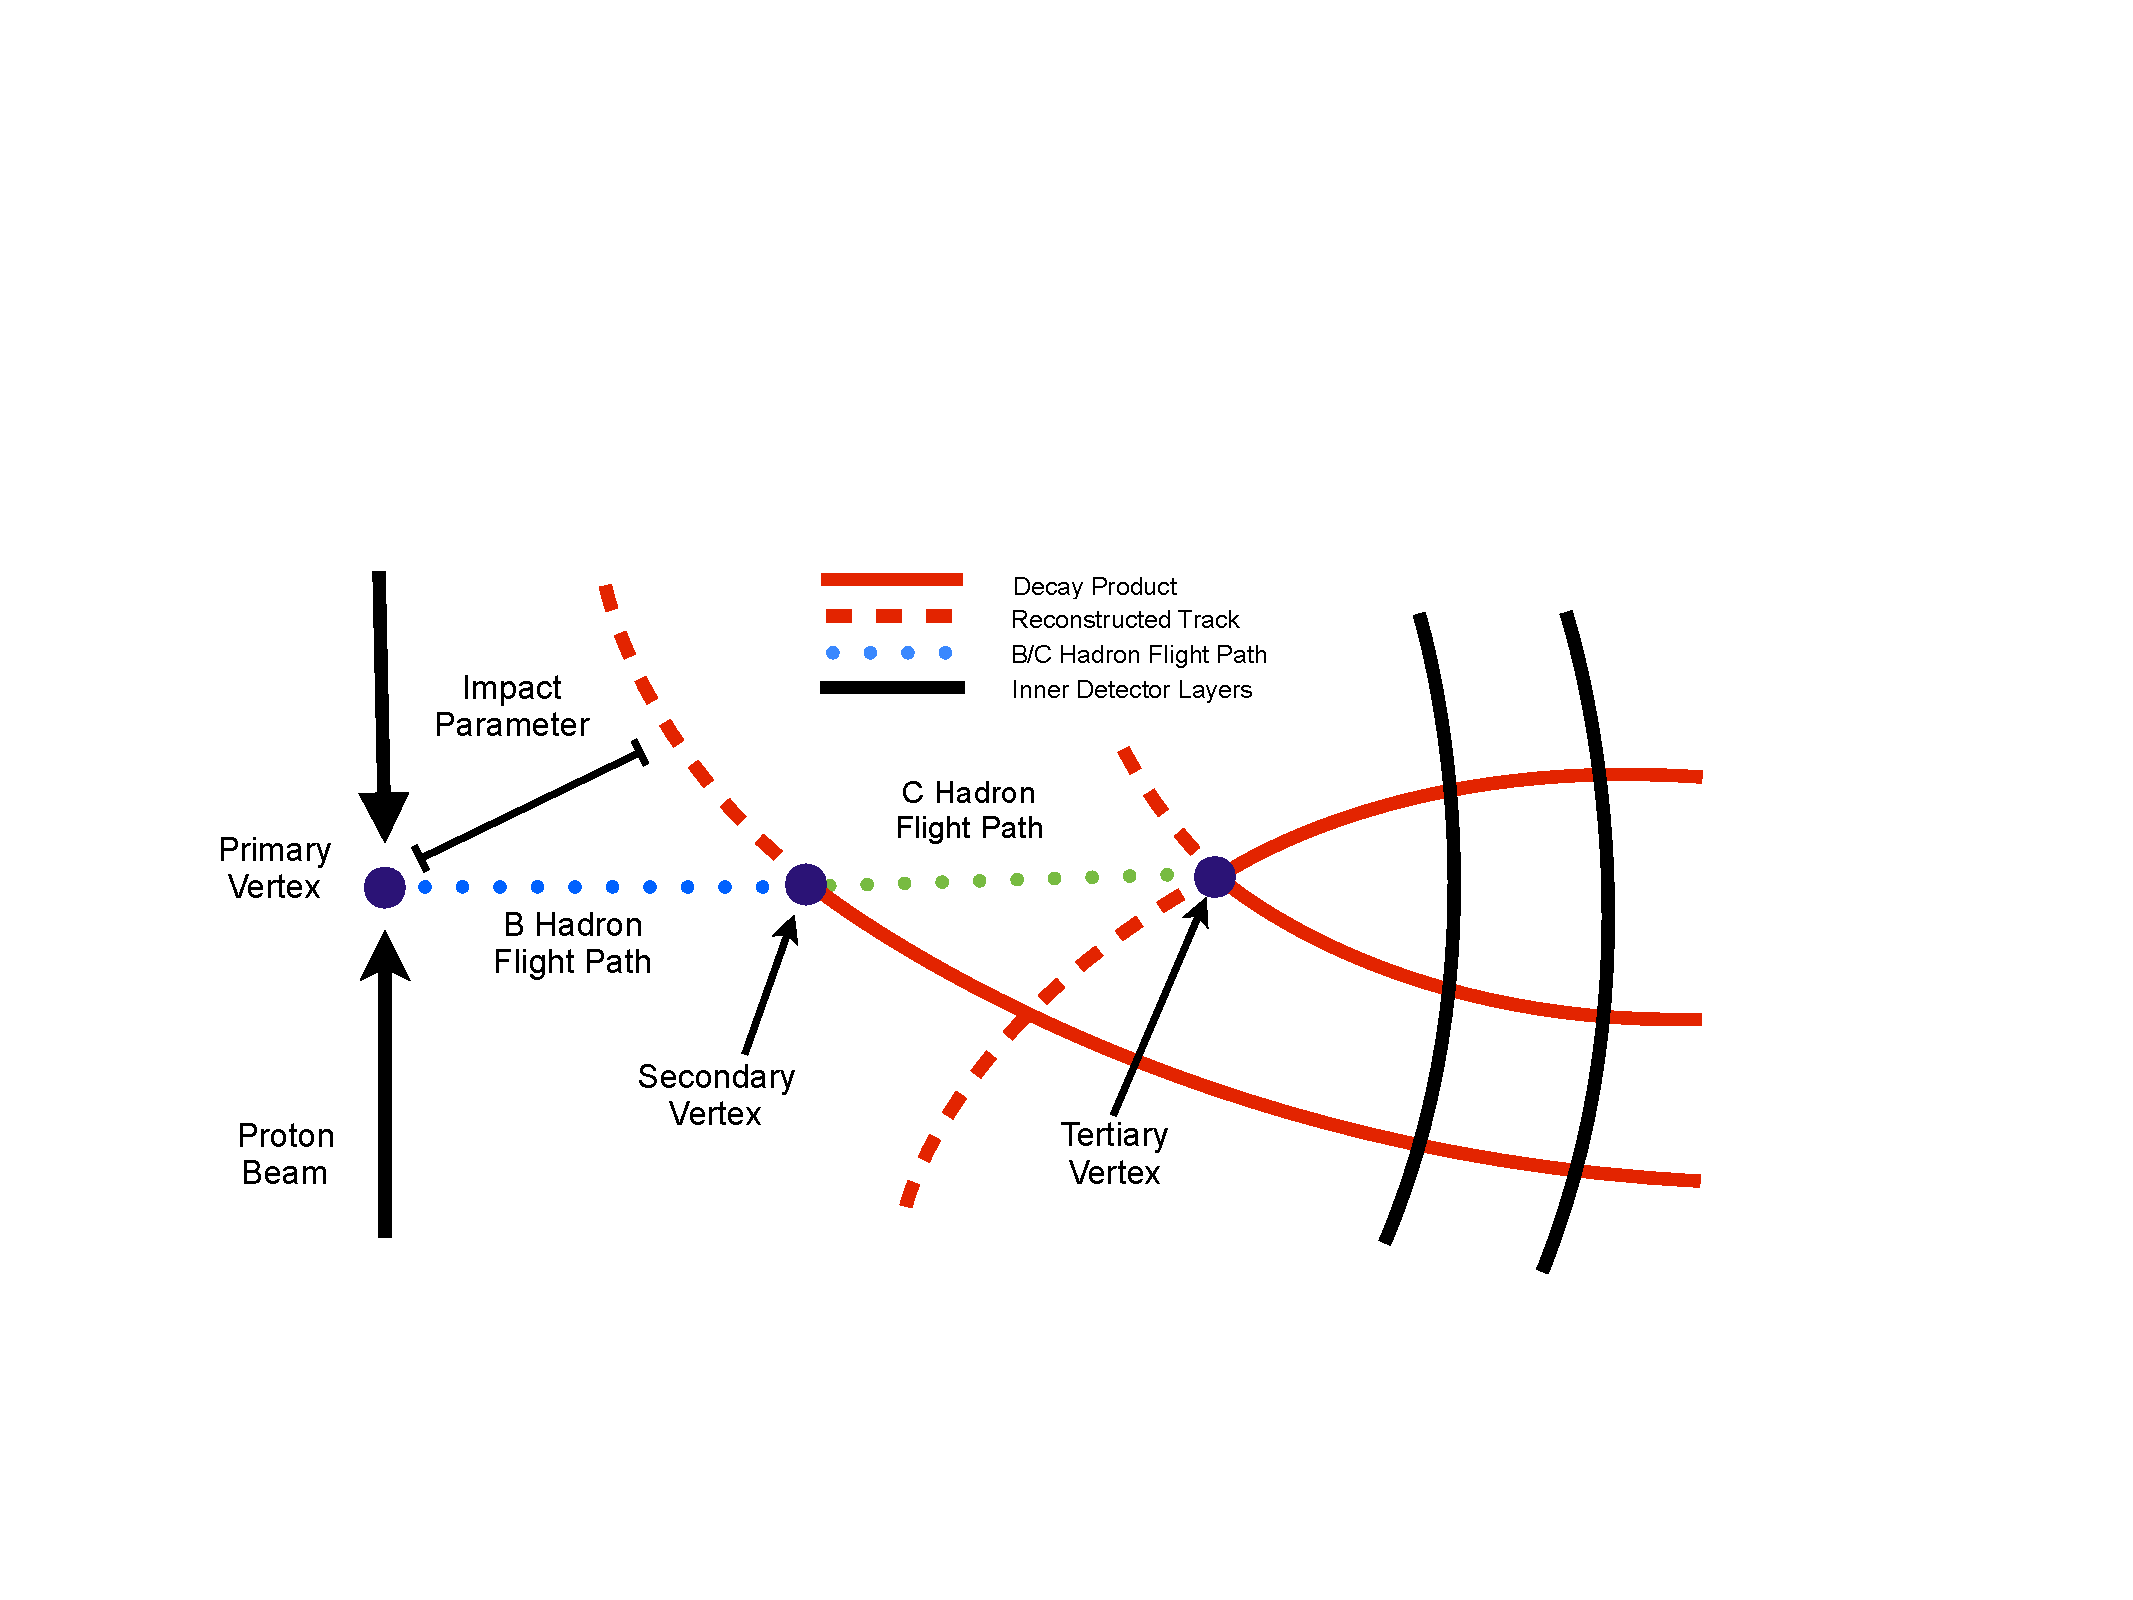
\includegraphics[width=0.9\textwidth]{figs/Objects/bjet_schem.pdf}
       \caption{A diagram to illustrate the key features of a $b$-jet that are utilised by the base $b$-tagging algorithms.}
       \label{fig:obj_bjet_schem}
     \end{center}
     \vspace{-0.5cm}
   \end{figure}

   \subsubsection{Impact parameter based}
   \label{sec:obj-bjets_IP}
 
   The IP3D algorithm is utilises the impact parameter, which is defined as the shortest distance between a specific track and the primary vertex.
   A track corresponding to a particle coming from the offset decay vertex of a heavy-hadron is likely to have a large impact parameter,
   meaning that the distribution of track impact parameter is different for each of the jet-flavours.
   The impact parameter of a track coming from the decay of a heavy hadron is indicated in Figure~\ref{fig:obj_bjet_schem}.
   In this algorithm, for all tracks associated to a jet, the impact parameter is calculated in both the transverse (perpendicular to beam-line)
   and longitudinal (parallel to beam-line) direction, which are referred to as $d_{0}$ and $z_{0}$.
   Then the IP3D algorithm calculates a likelihood of the jet having a specific flavour, 
   based on the distributions of the impact parameters ($d_{0}$, $z_{0}$) and their significances 
   ($d_{0}/\sigma _{d0}$ and  $z_{0}/\sigma_{z0}$) for tracks within the jet. 
   Another similar algorithm, IP2D, also calculates the jet flavour likelihood from just the transverse distributions, ($d_{0}$ and $d_{0}$ significance), which is more
   robust to pile-up, as tracks from pile-up jets are likely to have a large $z_{0}$ significance value.
   
   \subsubsection{Secondary vertex}
   \label{sec:obj-bjets_SV}

   
   The SV1 algorithm aims to reconstruct a secondary vertex of two or more intersecting tracks, corresponding to the decay of a heavy-flavour hadron;
   the secondary vertex within a $b$-jet's decay chain is illustrated in Figure~\ref{fig:obj_bjet_schem}.
   The SV1 algorithm then calculates many variables that are associated with properties of the reconstructed secondary vertex that show flavour discrimination;
   some example variables are the vertex invariant mass,
   which will be larger for $b$-jets due to the heavy mass of the $b$-hadron
   \footnote{Mass of a B-meson $\sim$ 5 GeV and the mass of a D-meson $\sim$ 1.9 GeV, which are the most common heavy hadrons in a $b$- and $c$-jet respectively.}, 
   the distance in the transverse plane between the primary vertex and the secondary vertex, % (2D flight path $L_{XY}$),
   which will be larger for $b$-jets due to the long lifetime of the $b$-hadron,
   and the number of tracks at the secondary vertex, which will be larger for reliable secondary vertices.
   
   \subsubsection{Jet Fitter}
   \label{sec:obj-bjets_JF}

   The JetFitter algorithm (JF) attempts to reconstruct the full decay chain of the $b$-hadron into a charmed-hadron and then into light-hadrons. 
   This is done by assuming that all vertices lie on a common $b$-flight axis, and then constructing vertices from the intersection of
   one or more tracks and the flight axis.
   The aim of this is to reconstruct the secondary and tertiary vertices which correspond to the decays of the $b$-hadron and charmed-hadron,
   as illustrated in Figure \ref{fig:obj_bjet_schem}.
   Similar to SV1, the JetFitter algorithm then calculates a number of flavour discriminating variables:
   for example vertex mass and number of vertices with two or more tracks.
   
   \subsubsection{Multi-variate}
   \label{sec:obj-bjets_MV2}

   The three base algorithms are combined in a boosted decision tree (BDT), a machine-learning technique for combining the many flavour-discriminating variables,
   resulting in an algorithm that is known in MV2
   As shown in Figure \ref{fig:obj-MV2_schem}, MV2 combines the likelihood output of IP3D and IP2D
   with the discriminating variables of SV1 and JF discussed in the preceeding sections,
   resulting in an output between -1 and 1, where 1 indicates that the jet is likely to be a $b$-jet and -1 indicates the inverse.

   A cut is then applied to this MV2 output in order to select jets that are likely to $b$-jets.
   The cut can be varied to create different working points which vary the $b$-jet efficiency, light-jet rejection and $c$-jet rejection
   \footnote{$b$-jet efficiency is defined as the probablitity of accepting a true $b$-jet.
     Light-jet rejection is defined as 1 divided by the probablity of accepting a true light-jet.
     A similar definition applies for $c$-jet rejection.}.
   Looser working points have a relatively low cut on MV2, meaning that the $b$-jet efficiency is higher at the cost of worse light- and $c$-jet rejections,
   and the inverse is true for tighter working points.
   Table~\ref{tab:obj-MV2_WPs} shows the list of fixed cut working points that are used in ATLAS defined by their $b$-jet efficiencies;
   the corresponding $c$-jet rejection rate, light-jet rejection rate and MV2 cut are also shown.
   \footnote{In this thesis only the fixed-cut working points shown obove will be used,
     however, there also exists a set of flat efficiency working points where the MV2 cut depends on jet-\pT}
   %This is in contrast to the previous multivariate tagger used in Run-1, MV1, which inputted
   %the likelihood of a jet having a certain flavour from each of the three base algorithms separately.

   \begin{figure}[!htb]
     \begin{center}
       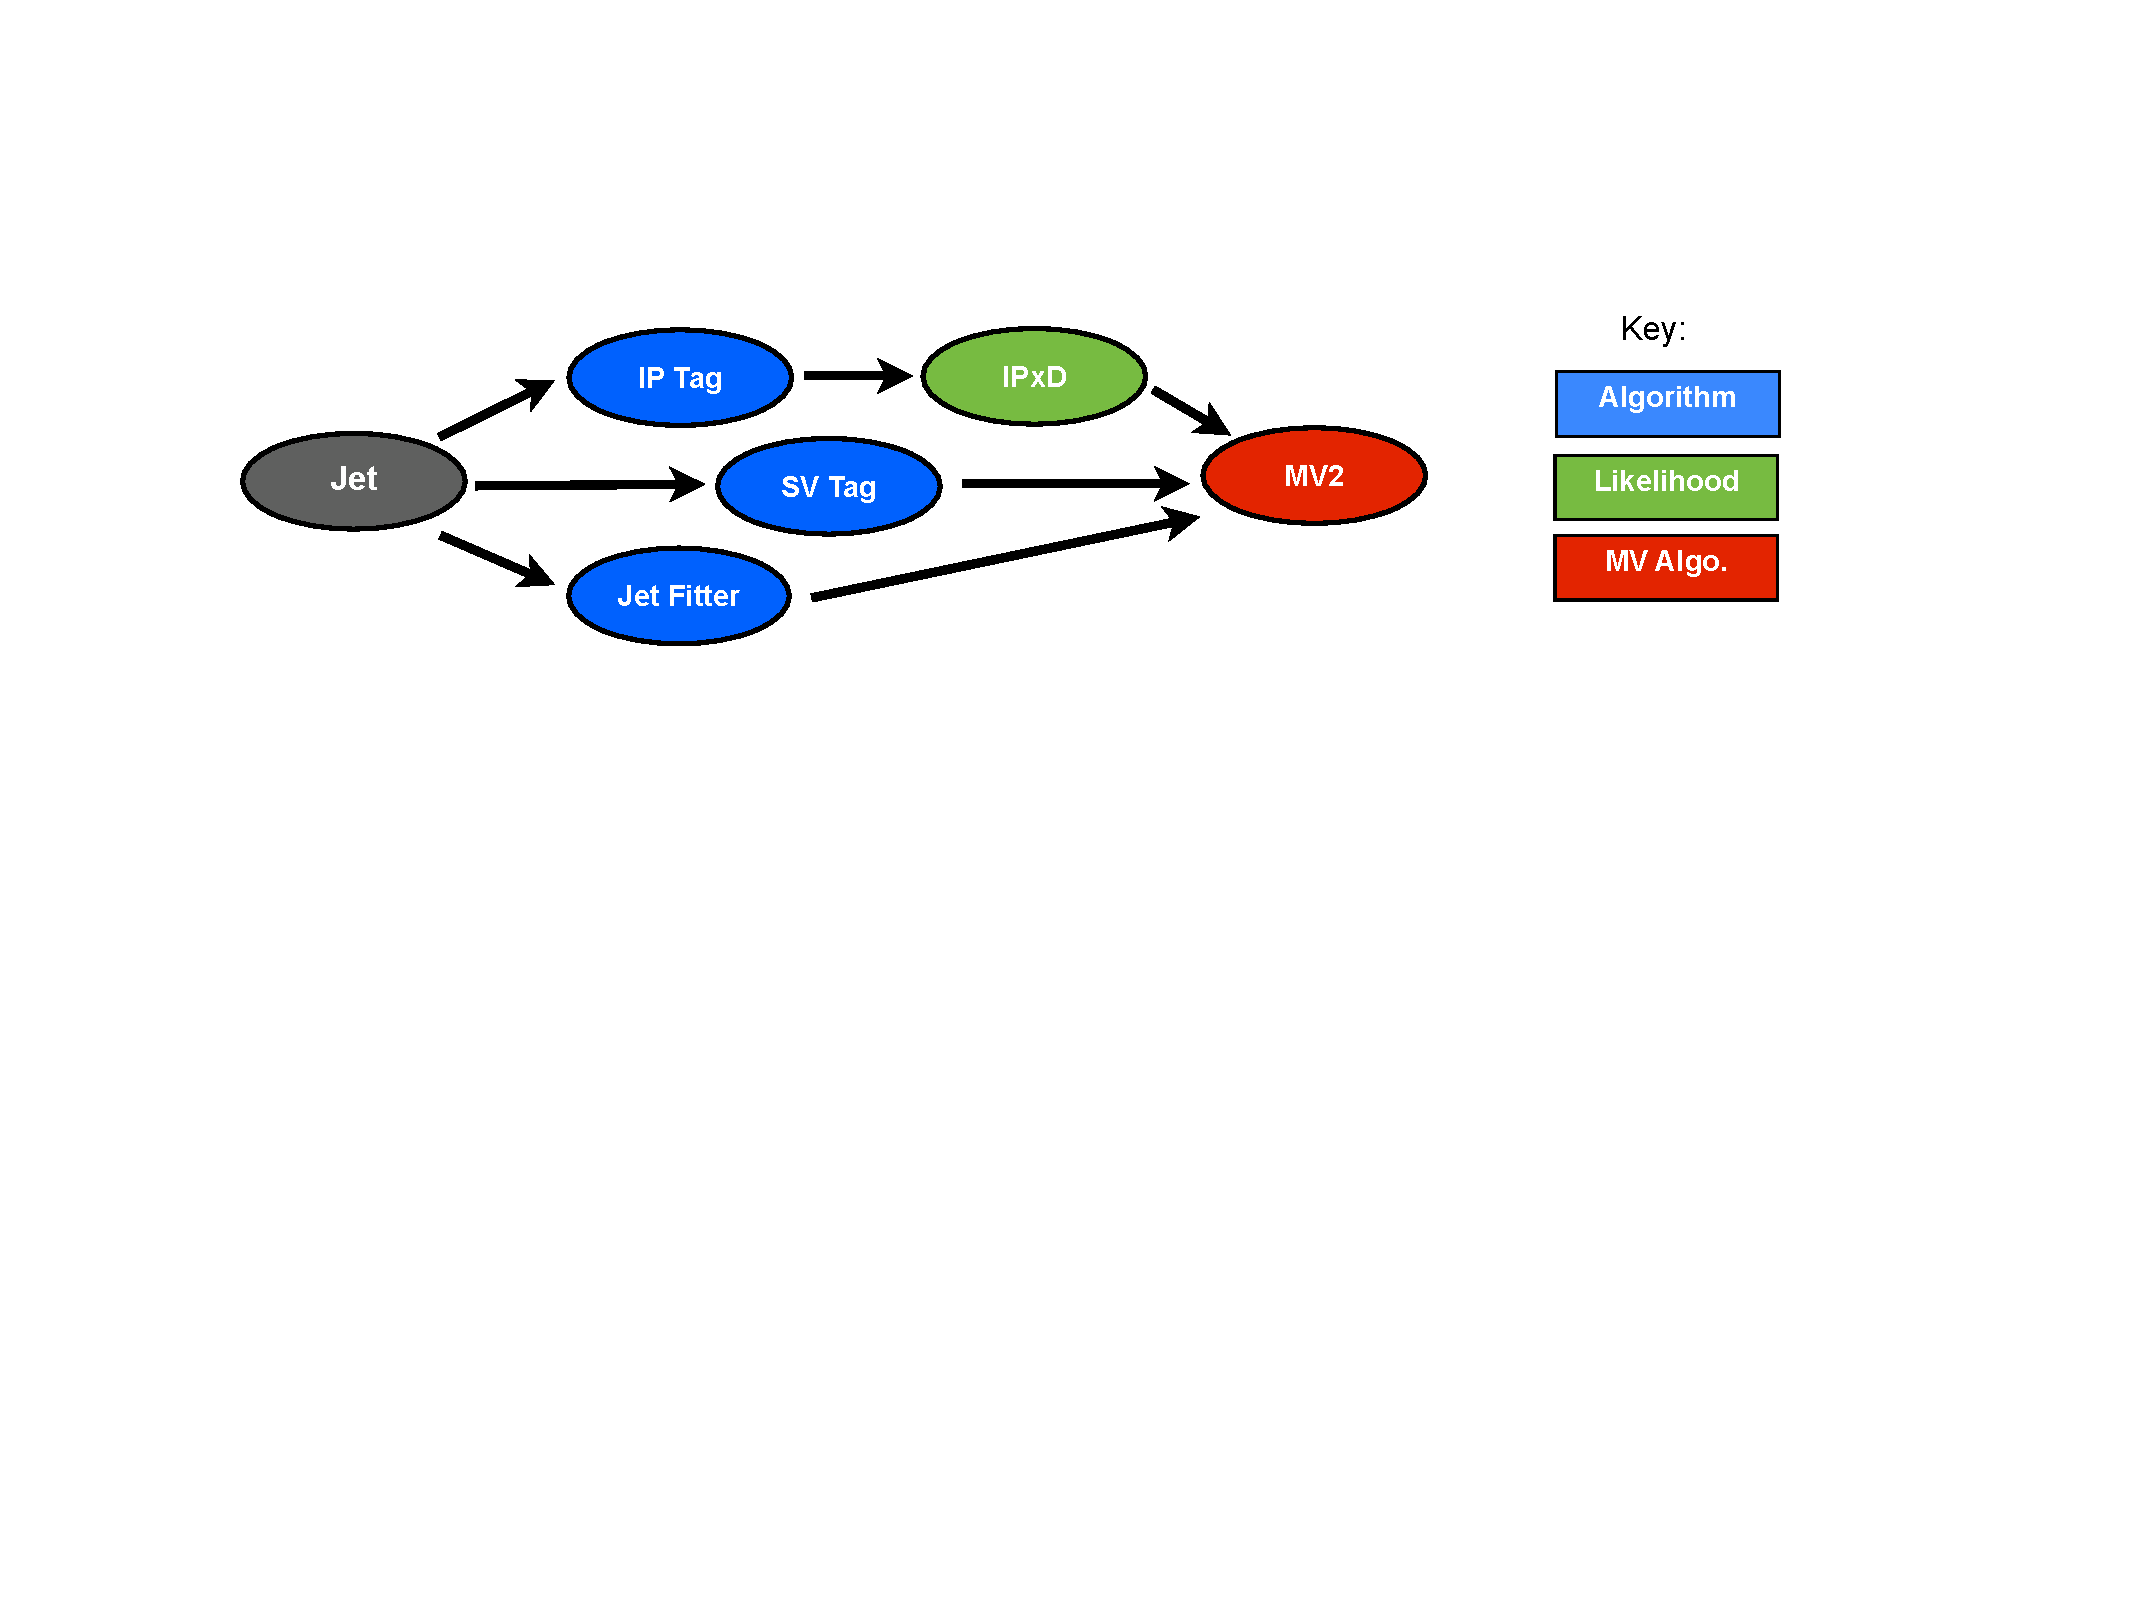
\includegraphics[width=1.0\textwidth]{figs/Objects/MV2_schem.pdf}
       \caption{A diagram showing how the three base flavour tagging algorithms are combined in the MV2 algorithm.}
       \label{fig:obj-MV2_schem}
     \end{center}
     \vspace{-1cm}
   \end{figure}
   
   The BDT is trained using a simulated sample of $t\bar{t}$ events that will contain a mix of  $b$-, $c$- and light-jets
   as well as a sample containing $Z'$ boson decaying to $b$-quarks.
   The training makes use of the truth flavour labels assigned to jets using the process described in Section~\ref{sec:obj-bjets_label}.
   A training sample with known truth labels is required as this allows the BDT to be optimised
   such that it uses the complex correlations between the input variables to allow for high $b$-jet efficiencies
   whilst still obtaining a large $c$- and light-jet rejection.
   The recommended $b$-tagging tool is MV2c10 which has been trained on a sample containing 10\% charm-jets, to give strong light- and $c$-rejection rates.
   
 
   
   \subsection{Calibration/performance}
   \subsection{bTagging: Validation in Dijet Events}
    
  \section{Leptons}   
  \subsection{Electron}
  \label{sec:obj-electron}
  \subsection{Muon}
  \label{sec:obj-muon}
    

\chapter{Triggering in the di-$b$-jet analysis}
\label{sec:trig}

As described in Section~\ref{sec:det-trig},
ATLAS does not have the resources to process and store all the data from the 40~MHz of collisions delivered by the LHC.
To solve this problem the ATLAS trigger system performs the vital role of
reducing the rate of data-taking to 1~kHz by selecting events containing a high-$p_T$ object. 

As a result all analyses must chose a trigger strategy and understand the impact of this trigger on their analysis.
In the di-$b$-jet analysis a single jet trigger is used for the high-mass channel
and a double $b$-jet trigger for the low-mass channel.
This chapter aims to provide a detailed description of the triggers used in this analysis,
and as such is organised in the following manner;
Section~\ref{sec:trig-jet} provides a brief description of jet triggers as used in the high-mass channel and the limitations of this approach,
Section~\ref{sec:trig-bjet} contains a description of $b$-jet triggers that are used in the low-mass channel
and finally Section~\ref{sec:trig-bjet_eff} presents the measurement of the $b$-jet trigger efficiency, an essential input of the low-mass channel.

\section{Jet-Triggers}
\label{sec:trig-jet}

Jet-triggers are tasked with selecting events with one or more jets from the deposits in the ATLAS calorimeter system,
this is one of most challenging triggers in any hadron-hadron collider due to the extremely high cross-sections of hadronic jet production~\cite{trig-run2_proc}.
In Run-2 the jet-triggers are used at both L1 and HLT level; each using different levels of information and different algorithms,
so are described separately within this section.

\subsection{Level 1}

The L1 trigger is a hardware based trigger which accepts or rejects an event within \SI{2.2}{\micro\second}.
The L1 jet-trigger receives trigger towers from the calorimeter;
where a trigger tower is the measured energy deposit in a cell of the ECAL or HCAL of granularity 0.1x0.1 in the $\eta-\phi$ plane.
In the L1 trigger hadronic jet algorithms search for a neighbouring group of 4x4 trigger towers containing energy deposits above some pre-set threshold.
Our analysis uses the L1 trigger known as \verb|L1_J100|, which requires that at least one trigger tower group with an energy deposit of \SI{100}{\GeV} has been found.
Other L1 triggers that search for multiple clusters are also possible to reduce the energy thresholds required.
The L1 trigger then seeds the HLT trigger.
It is also worth noting that at L1 there is no tracking information, meaning that electron and taus
are also triggered on using similar techniques as hadronic jet algorithms, except using narrower groups of trigger towers.


\subsection{HLT}

The HLT trigger is a software based trigger which, due to the lower input rate and larger time window,
is able to use more complex algorithms to reconstruct jets.
At the HLT level jets are reconstructed using topoclusters (TCs) constructed from neighbouring cells selected using the cell's energy significance ($E/\sigma$);
TCs are seeded from cells with $E/\sigma > 4$, then neighbouring cells with $E/\sigma > 2$ are added
and finally all neighbouring cells around are also added.
Jets are then reconstructed from the topoclusters;
in this analysis jets have been reconstructed using
the anti-$k_T$ algorithm with an $R = 0.4$ \footnote{Section~\ref{sec:obj-jets} \textit{(sec:obj-jets)} defines these terms}. 

\subsection{High-mass trigger selection}

For the high-mass analysis the trigger \verb|HLT_j380| is used, that is fired when a jet is found with a $p_T >$ 380 GeV.
This is chosen as it is the lowest un-prescaled single jet-trigger;
meaning that of triggers that accept every event passing a single jet criteria,
this trigger has the lowest jet-$p_T$ threshold.
Due to the exponential increase in jet production cross-section at low jet-$p_T$,
the $p_T$ threshold is set to keep the acceptance rates low enough such that the HLT trigger is within its output rate budget of 1~kHz.

However, as will be discussed further in Section~\ref{sec:evtSel}\textit{(sec:evtSel)},
this $p_T$ threshold limits the high-mass di-$b$-jet analysis to only select events with $m_{jj} >$ 1.2~TeV.
Otherwise the $m_{jj}$ range will enter a kinematic region where
trigger acceptance is less than 1 in such a way that the QCD background is sculpted
in a manner that the background modelling can not adapt to.
To reach lower masses a different trigger strategy is required.

\section{$b$-Jet Triggers}
\label{sec:trig-bjet}

This analysis searches for pairs of $b$-jets,
which, as described in Section~\ref{sec:obj-bjets}\textit{(sec:obj-bjets)},
can be identified from the topology of tracks in the inner detector indicating that a $B$-hadron was within the jet.
The same techniques can be used at the trigger level to reduce rates significantly
\footnote{It is known that the QCD background is dominated by light-jets, see Figure~\ref{fig-dibjet_backgroundFlav}\textit{Plot of background flav comp}}
allowing a lower jet-$p_T$ threshold than was used by the single jet-$p_T$ trigger, and hence lower $m_{jj}$ values to be accessed.
$b$-jet triggers have been used in a range of previous ATLAS analyses
including for searches for exotic particle decaying into a pair of Higgs bosons, which then decay to 4 $b$-jets~\cite{trig-H4b}.

\subsection{General description}

In 2016 data, the $b$-jet trigger configuration contains three steps~\cite{trig-bTrig_desc},
making use of the regions of interest (RoI) described by the jets found by the jet-trigger.
Firstly, a `fast'-tracking algorithm is run in a super-RoI
which is formed around all jets in the event which have $E_T >$ 30 GeV;
these tracks are then used to identify the primary vertex in the event.
Secondly, within each jet RoI precision tracking is run, with a constraint on the PV position from the first step.
Finally, these tracks are the input to the multi-variate $b$-tagging algorithm described in
Section~\ref{sec:obj-bjets_MV2}\textit{(sec:obj-bjets\_MV2)} to identify $b$-jets.
There are several $b$-jet triggers available in the ATLAS trigger menu;
with a variety of requirements on the jet multiplicity, number of tagged jets and $b$-tag operating point used.
Figure~\ref{fig:trig-bTrig_perf} shows ROC curves representing the expected performance of the Run-2 $b$-jet trigger.


\begin{figure}[!ht]
  \begin{center}
    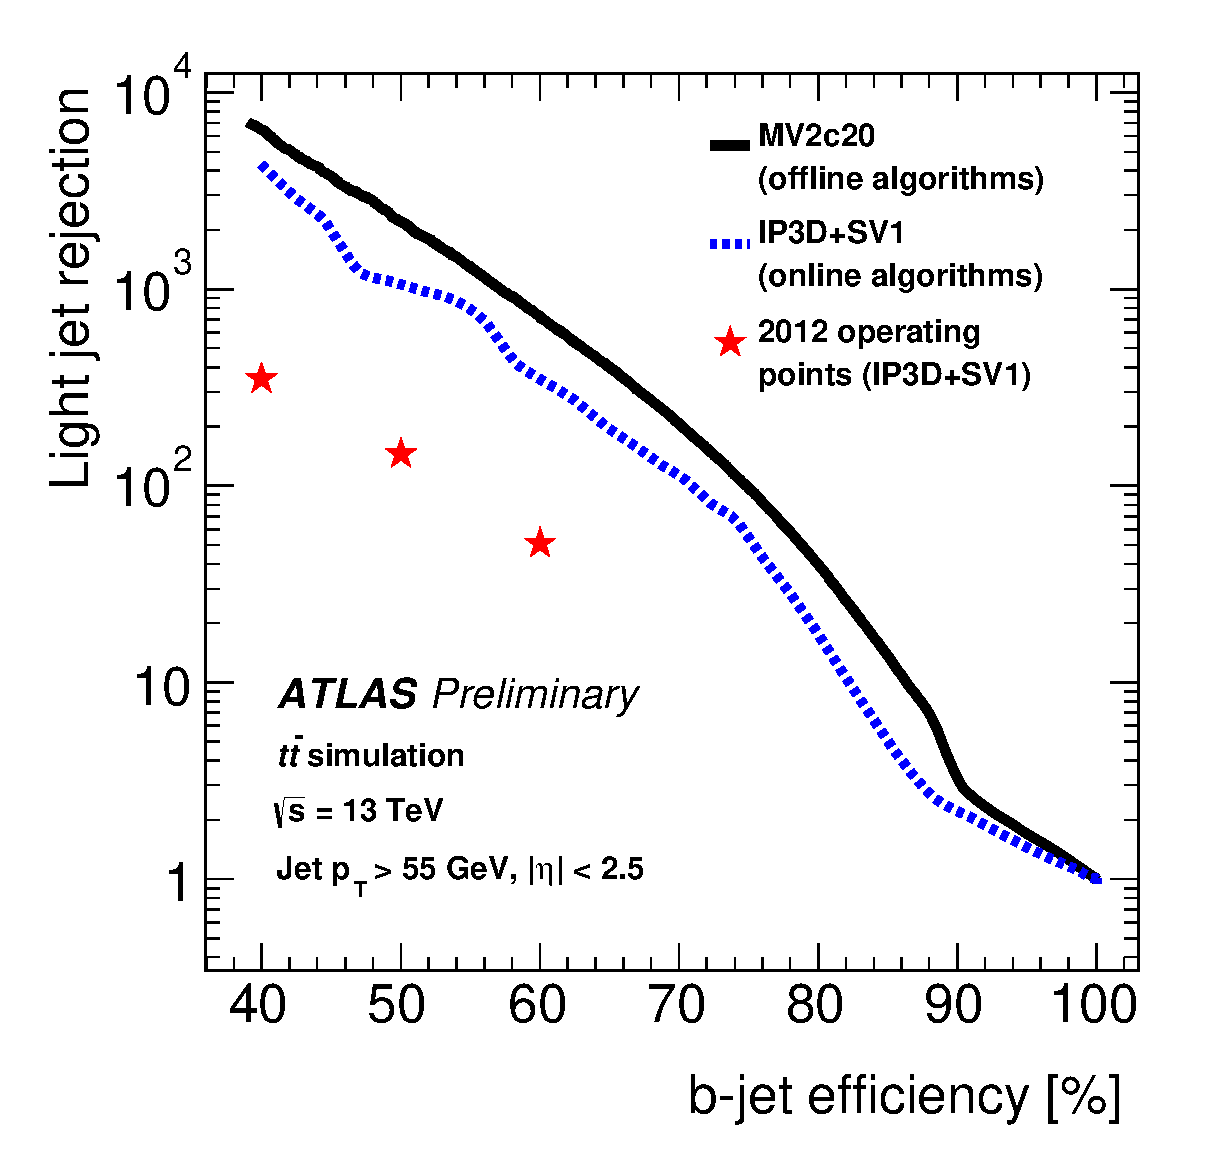
\includegraphics[width=0.48\linewidth, angle=0]{figs/Trigger/trig-bTrig_perf_light.eps}
    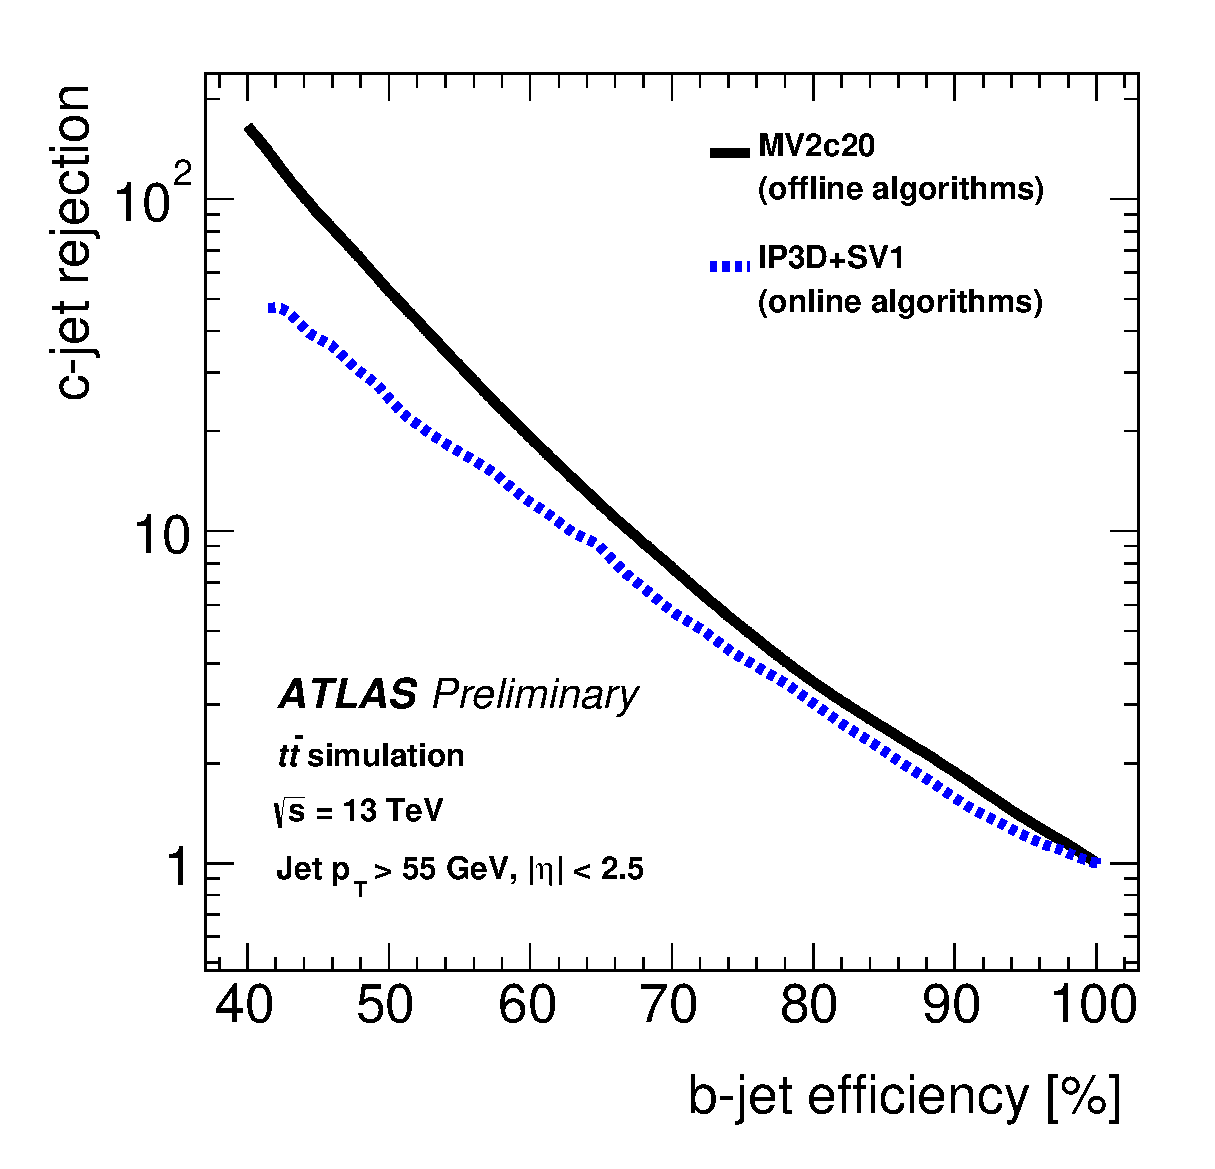
\includegraphics[width=0.48\linewidth, angle=0]{figs/Trigger/trig-bTrig_perf_charm.eps}
  \end{center}
  \caption[The expected $b$-jet efficiency of $b$-jet triggers with respect to (a) light-jet and (b) $c$-jet rejection
    in the case where the $b$-tagging algorithm used is MV2c20 (Black), IP3D+SV1 (Blue) and for the set-up used in Run-1 (red stars)]
    {The expected $b$-jet efficiency of $b$-jet triggers with respect to (a) light-jet and (b) $c$-jet rejection
    in the case where the $b$-tagging algorithm used is MV2c20 (Black), IP3D+SV1 (Blue) and for the set-up used in Run-1 (red stars)~\cite{trig-bTrig_desc}.}
  \label{fig:trig-bTrig_perf}
\end{figure}

There are few subtleties worth commenting on the $b$-jet trigger configuration which affect decisions taken in this analysis.
One is that on this figure there are two lines corresponding to different $b$-tagging algorithms used in $b$-jet trigger;
IP3D+SV1 was used in 2015 data-taking,
whilst the MV2c20 was used in 2016 data-taking.
Another difference between 2015 and 2016 is the primary vertex finding algorithm used;
2016 data-taking employed an algorithm based on offline primary vertex finding, know as \verb|xPrmVtx|,
whilst in 2015 an algorithm using a simpler histogram based approach was employed, known as \verb|EFHist|. 

Finally it is worth noting that there are  differences between online and offline $b$-tagging that will have an impact on what is to follow.
Firstly, coarser tracking information is available online, notably online tracks are not reconstructed from the whole range of the detector.
Secondly, a slightly different training setup is used for the multi-variate algorithm, mainly that a different fraction of $c$-jets were present in the training sample
(10\% offline vs. 20\% online).

In this analysis a double $b$-jet trigger is used,
\begin{center}
\verb|HLT_j150_bmv2c2060_split_j50_bmv2c2060_split|
\end{center}
which triggers on two jets with $p_T >$ 150 and 50 GeV respectively,
which have been $b$-tagged at the 60\% efficiency working point.

\newpage

\section{Efficiency Measurement of the $b$-Jet Trigger}
\label{sec:trig-bjet_eff}

Any part of the ATLAS detector framework needs to be understood and calibrated with data for use in an analysis;
and this includes the trigger which can have a large impact on the analysis.
In this section I discuss the strategy and results of the $b$-jet trigger efficiency measurement in 2016,
which is an important input to the low-mass channel of the di-$b$-jet analysis.

For clarity in this section I would like to make two definitions clear.
Online refers to any algorithms run or objects reconstructed at the trigger level,
offline refers to algorithms run after events have passed the trigger at the data-processing level. 

\subsection{Strategy}
The $b$-jet trigger is always used in tandem with offline $b$-tagging which is calibrated independently of the $b$-trigger.
As mentioned before, there are many differences between offline and online $b$-tagging.
Hence, to do this measurement whilst making use of the offline $b$-tagging calibrations already available,
$b$-jet trigger efficiency with respect to offline $b$-tagging, $\epsilon_{bTrig}$, is measured.
This is defined as the number of offline-tagged true $b$-jets that match an online-tagged trigger-jet
divided by the number of offline tagged $b$-jets that match a trigger jet.
Or to put this in an equation;
\begin{equation}
 \epsilon_{bTrig} = \frac{N(\text{Offline-tagged, online-tagged, true $b$-jets)}}{N(\text{Offline-tagged, trigger-matched, true $b$-jets)}}
\end{equation}
This quantity can be interpreted as the probability that a true $b$-jet is tagged at the trigger-level,
given that it there is a jet at the trigger level and that it would be $b$-tagged at the offline stage.

To measure $\epsilon_{bTrig}$ a sample that has high $b$-jet purity is required,
such that jets used to calculate this ratio are true $b$-jets.
It is also necessary to trigger on this sample in such a way that there is no bias from using $b$-tagging online;
or simply put the $b$-jet trigger cannot be used to select events.
The sample used to fill these criteria is a di-lepton $t\bar{t}$ sample containing a muon and an electron.
Top-quarks decay to a $W$-boson and a $b$-quark with almost 100\% branching ratio meaning that this sample provides a good source of $b$-quarks,
but also the electron and muon give a distinct signature which allows us to select this process with good purity and gives a non-$b$-jet object to trigger on.
The exact event selection is described below. 

The $b$-jet trigger efficiency is determined in data and is compared to the efficiency found in a 
simulated $t\bar{t}$ sample which is used to extrapolate the efficiency to 
higher jet-$p_T$ where the data-derived efficiency loses statistical precision.
The efficiency in data, including the simulation based extrapolation, can then be
compared to simulation to derive a Data/Monte-Carlo scale factor, which is used as the input to the analysis.


$\epsilon_{bTrig}$ and Data/Monte-Carlo scale factors are derived for all combinations of offline and online $b$-tagging working points.
However, only the process for the 70\% offline and 60\% online working point is shown
as this is set of working points used in this analysis.

\subsection{Datasets}
The data used for this analysis is the full 2016 ATLAS data-set.
In addition to the usual data-quality requirements applied,
as discussed in Section~\ref{sec:evtSel_GRL}\textit{(sec:evtSel\_GRL)},
a $b$-jet trigger aware Good Run List (GRL)
\footnote{A GRL is effectively a list of lumi-blocks that pass certain data-quality requirements.
 As mentioned in the text a further discussion is held here in Section~\ref{sec:evtSel_GRL}\textit{(sec:evtSel\_GRL)}}
applies the requirement that the online beamspot $z$-position is within 2mm of the origin in Periods A-I of the data.
This means that the data-set contains 24.5~\ifb~of data.
A discussion of the requirement for this GRL is in Section~\ref{sec:trig-inv}. 

For the simulated $t\bar{t}$ sample, the generation is performed with
a Powheg-Box v2~\cite{trig-powheg} generator with the CT10 PDF sets in the matrix element calculations.
Also considered is a simulated single-top sample;
electroweak t-channel, s-channel and $Wt$-channel single top-quark events are generated using the Powheg-Box v1 generator.
This generator uses the 4-flavour scheme for the NLO matrix elements calculations together with the fixed four-flavour PDF set CT10f4.
%For all top processes, top-quark spin correlations are preserved (for t-channel, top quarks are decayed using MadSpin[10a]).
For both processes the parton shower, fragmentation, and the underlying event are simulated using Pythia6.428~\cite{trig-pythia6} with the CTEQ6L1~\cite{trig-CTEQ6L1} PDF sets
and the corresponding Perugia 2012 tune (P2012)~\cite{trig-perugia}.
The top mass is set to 172.5 GeV.
The EvtGen v1.2.0 program~\cite{trig-evtGen} is used for properties of the bottom and charm hadron decays. 
\newpage

\subsection{Event Selection}
\label{sec:trig-evtSel}

A high-purity sample of $b$-jets is selected using a di-lepton $t\bar{t}$ selection.

\noindent
The event selection is summarised as follows:

\begin{itemize}
\item The event fired a single lepton bperf trigger which are:
    \begin{itemize}[label={$-$}]
      \item\verb|HLT_mu26_imedium_2j35_bperf|
      \item\verb|HLT_e26_tight_iloose_2j35_bperf|
      \item\verb|HLT_e26_lhtight_iloose_2j35_bperf|
    \end{itemize}
\item At least 1 medium muon: $\pT>25~\GeV$, which has no jet within a $\Delta R$ of 0.4.
\item At least 1 medium electron: $\pT>25~\GeV$.
\item 2 offline $b$-tagged jets, defined as:
   \begin{itemize}[label={$-$}]
     \item Offline R=0.4 anti-$k_T$ jets.
     \item $\pT>35~\GeV$ and $|\eta|<2.5$.
     \item Offline $b$-tagged at the 85\%~operating point.
     \item Jet must be matched to a trigger-jet.
    \end{itemize}
\end{itemize}
\vspace{1em}

Descriptions of the object-definitions of muons, electrons, jets and $b$-tagged can be found in
Sections~\ref{sec:obj-muon}\textit{(sec:obj-muon)},~\ref{sec:obj-electron}\textit{(sec:obj-elec)},~\ref{sec:obj-jets}\textit{(sec:obj-jet)}
and \ref{sec:obj-bjets}\textit{(sec:obj-bjet)} respectively.
Online trigger jets are matched exclusively to offline jets using $\Delta R$ matching, requiring for a match the jets must have $\Delta R<0.6$.

The triggers used are bperf trigger, which are special triggers used in data-taking specifically for monitoring the $b$-jet trigger performance.
They fire if a muon or an electron with $\pT > 26$~\GeV~is reconstructed at the trigger level.
The bperf triggers then run the online $b$-tagging algorithm on all trigger jets with $|\eta|<2.5$ and
$p_{T}>35$~\GeV~without performing any cuts on the output of the multi-variate algorithm; ensuring there is no bias in the efficiency measurement. 


\newpage

\subsection{The Initial Problem}
\label{sec:trig-initProb}

To give context to the following section;
the first discussion will be what was first observed when measuring the $b$-jet efficiency.
To show the problems observed clearly, in this section the initial event selection is replicated;
hence  no $b$-jet trigger aware GRL is applied, offline jets are not required to match a trigger jet in the denominator
and the triggers required are single lepton triggers without the additional $b$-perf functionality
\footnote{Specifically HLT\_mu26\_imedium, HLT\_e26\_tight\_iloose and HLT\_e26\_lhtight\_iloose. }.
In addition, for this and the following two sections simulation refers to $t\bar{t}$ only,
but it will be shown later that the effect of single-top production is small so the conclusions here are still valid. 

Figure~\ref{fig:trig-Full_noGRL_eff_noHLTMatch} shows $\epsilon_{bTrig}$ against jet-\pT~and jet-$\eta$;
the efficiency in data is substantially below the efficiency expected from simulation and shows a clear shape in jet-$\eta$ distributions.
This substantial differences need to be investigated and understood. 

\begin{figure}[!ht]
  \begin{center}
    \captionsetup[subfigure]{aboveskip=0pt,justification=centering}
    \subcaptionbox{Jet-\pT}{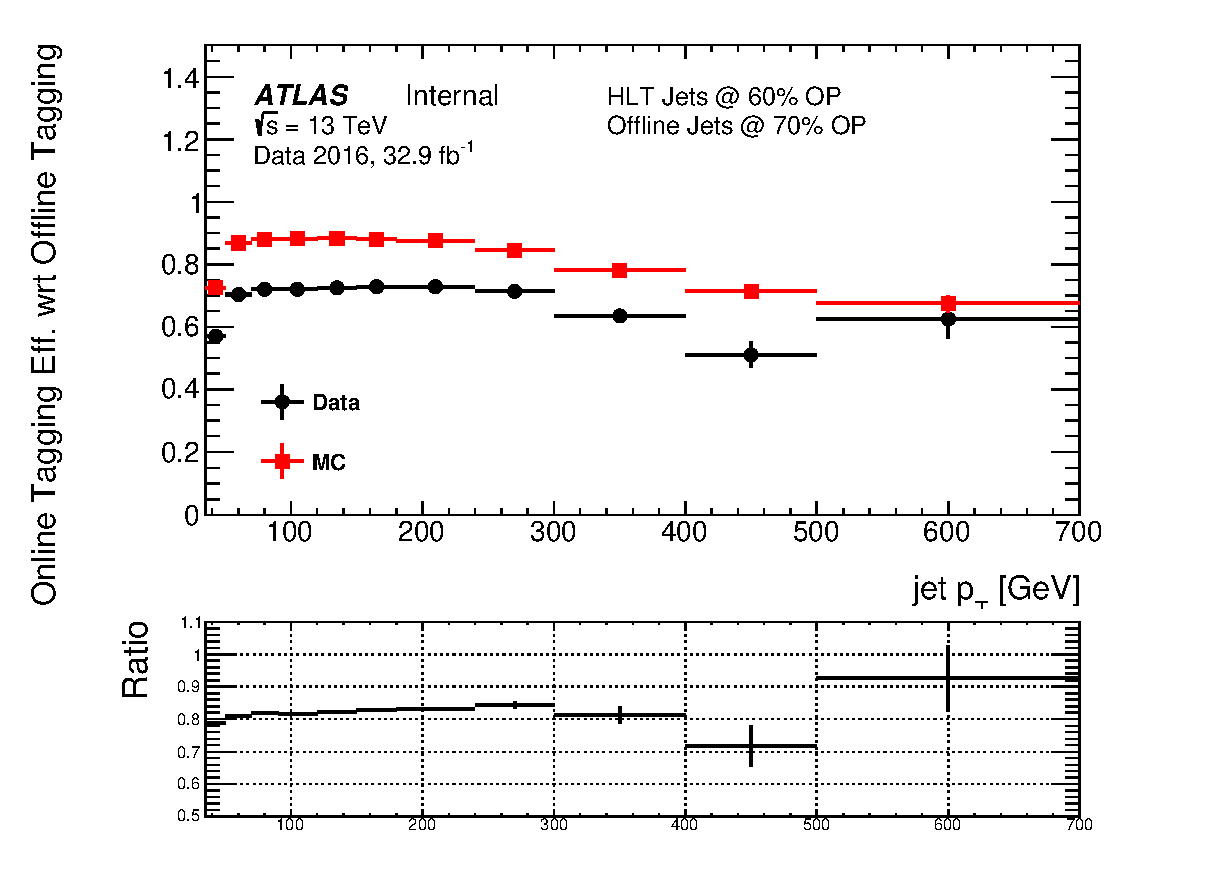
\includegraphics[width=0.48\linewidth, angle=0]{figs/trigger/Full_noGRL_eff_noHLTMatch_jetPt.eps} }
    \subcaptionbox{Jet-$\eta$}{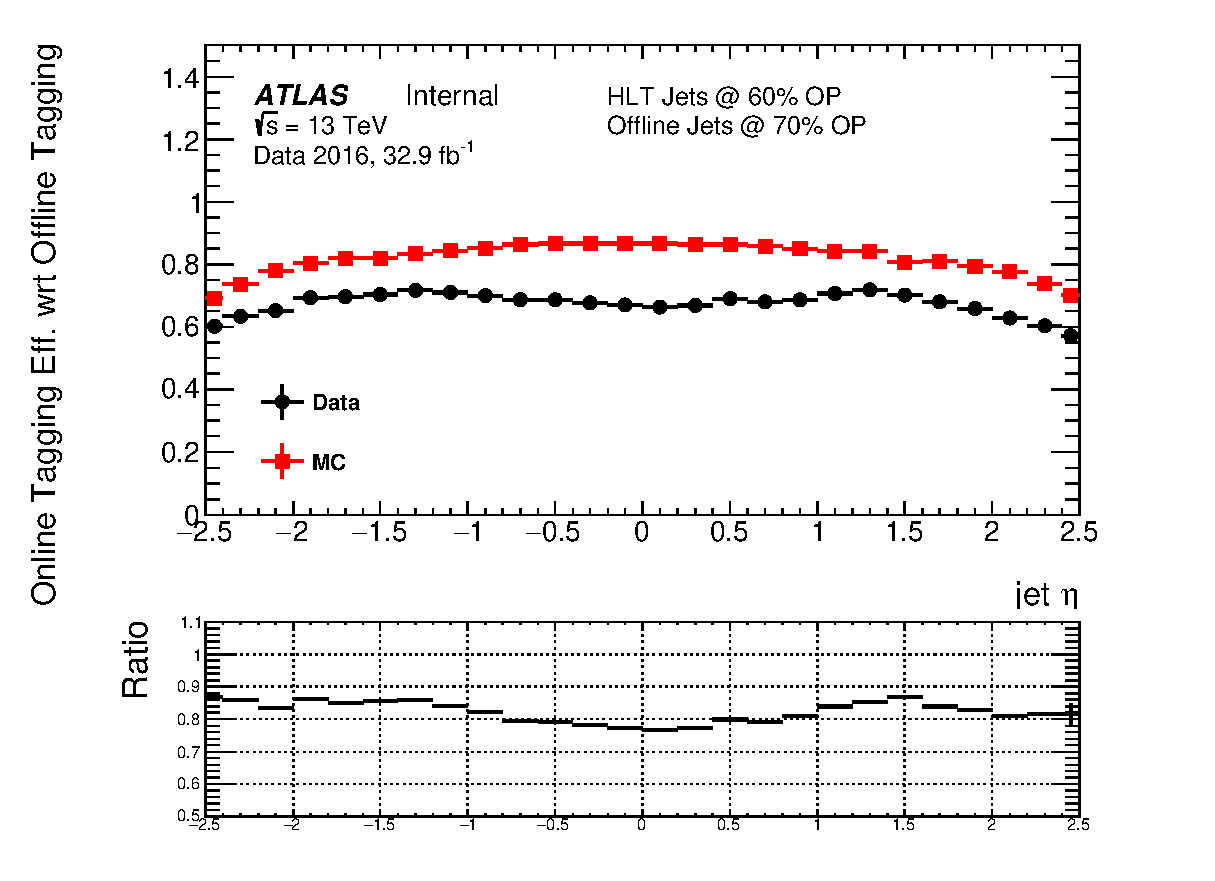
\includegraphics[width=0.48\linewidth, angle=0]{figs/trigger/Full_noGRL_eff_noHLTMatch_jetEta.eps}}
  \end{center}
  \caption{The 60\% $b$-jet trigger efficiency with respect to an offline 70\% operating point tag
    for Data (black) and simulation (red) against jet-\pT~(a) and jet-$\eta$ (b).
    The $b$-trigger aware GRL is not applied and trigger matching is not required.}
  \label{fig:trig-Full_noGRL_eff_noHLTMatch}
\end{figure}

\subsection{Investigation}
\label{sec:trig-inv}

Given the disagreements between data and simulation shown above
a number of cross-checks were performed to understand this discrepancy,
including checking for performance dependence on period,
detector performance, pile-up conditions and online beamspot position.
In this section, I summarise the results of the investigation
and our understanding of the $b$-trigger performance in 2016 data.
For this, the set-up as described in \ref{sec:trig-evtSel} is used
with the exception that the $b$-jet aware GRL is not applied to allow us to see the problems clearly.

The major problem that was discovered to be causing the large discrepancies was related to primary vertex finding.
As described above, in 2016 data an algorithm known as \verb|xPrmVtx| was used to find the primary vertex.
It has since been uncovered that there was a bug in the code used to implement this algorithm;
effectively different co-ordinates were used by different components of the code.
Online tracks passed to \verb|xPrmVtx| use position with respect to online beam-spot position,
where the \verb|xPrmVtx| algorithm assumed track position with respect to the origin.
This means that when the online beamspot $z$-position is far from from the origin,
a dummy vertex with position at the origin is passed to the $b$-tagging algorithms.
This leads to sub-optimal performance, as will be shown below.
For ease of reading online beamspot $z$-position is henceforth referred to as $z_{bs}^{online}$.  

The exact setup for the $b$-jet trigger has changed as data has been taken, to respond to performance issues as they are noticed and patches are applied.
As such the relevant conditions of the $b$-jet trigger can be split into three regions of data-taking, which I will refer to as epochs.
The effect of \verb|xPrmVtx| returning a dummy vertex on $b$-jet trigger performance is different in each of these epochs,
the details are summarised Table~\ref{tab:trig-epochs}.
As a result of these differences in trigger performance, each epoch is now considered independently.

\begin{table}[!htb]
  \begin{tabular}{ | c || c | c | c |}
    \hline			
    Epoch & Runs & Periods & Effect if no \verb|xPrmVtx| PV is found \\ \hline
    1 & \parbox[t]{2.5cm} {296939-300571,\\ 300655 \\}  & A,B(part)             & \parbox[t]{5cm} {\hspace{1mm}An invalid vertex is passed to the online b-tagging } \\
    \hline
    2 & \parbox[t]{2.5cm} {300600,\\ 300784-308084\\}  & B(part),C,D,E,F,G,I,J & \parbox[t]{5cm} {\hspace{1mm}The b-jet trigger is not fired\\ } \\
    \hline
    3 & \parbox[t]{2.5cm} {309331-311481\\}       & K,L                     & \parbox[t]{5cm} {\hspace{1mm}A back-up primary vertex \\ finding algorithm is used.\\} \\
    \hline
  \end{tabular}
  \vspace{10pt}
  \caption{A table describing the effect of not finding a valid xPrmVtx primary vertex on different epochs of data.}
  \label{tab:trig-epochs}
\end{table}
%For Epoch 1, the $\epsilon_{bPerf}$ is 100\% as shown in Figure~\ref{fig:Epoch1_bperf} for Period A.Figure~\ref{fig:Epoch1_eff} shows the $\epsilon_{bTrig}$ in Epoch 1,
Firstly let us consider Epoch 1;
Figure~\ref{fig:Epoch1_eff}(a) shows that efficiency against jet-\pT~is ~80-90\% of that in simulation, similar to that shown in the previous section.
However, Figure~\ref{fig:Epoch1_eff}(b) shows that $\epsilon_{bTrig}$ in Epoch 1 has a strong dependence of  $z_{bs}^{online}$;
when  $z_{bs}^{online}$ is close to zero $\epsilon_{bTrig}$ in data and simulation are comparable
\footnote{In simulation the  $z_{bs}^{online}$ is always set to zero.}
but as $|z_{bs}^{online}|$ increases efficiency falls off steeply.
To understand this performance the variable `vertex class' is studied, which is defined as 0 when a valid \verb|xPrmVtx| vertex is found and 1 if not.
Figure~\ref{fig:Epoch1_vtxClass}(a) shows that when an \verb|xPrmVtx| vertex is found $\epsilon_{bTrig}$ is reasonably high ($\sim$ 0.8) and is comparable between data and simulation (within 5\%),
whilst if no valid \verb|xPrmVtx| vertex is found then efficiency is very low in both simulation and data.
However, Figure~\ref{fig:Epoch1_vtxClass}(b) shows that a valid \verb|xPrmVtx| vertex is found in simulation in $> 99$ \% of the jets,
whilst in data there is $\sim$ 16\% of events where no valid \verb|xPrmVtx| vertex is found.
Hence, combining the information in Table~\ref{tab:trig-epochs}, Figure~\ref{fig:Epoch1_eff} and Figure~\ref{fig:Epoch1_vtxClass}
it can be concluded that in Epoch 1 in events where the  $|z_{bs}^{online}|$ is far from 0
then \verb|xPrmVx| returns an dummy vertex which results in a low $\epsilon_{bTrig}$, explaining the data/simulation differences in Epoch 1. 

\begin{figure}[!ht]
  \begin{center}
    \captionsetup[subfigure]{aboveskip=0pt,justification=centering}
    \subcaptionbox{Jet-\pT}{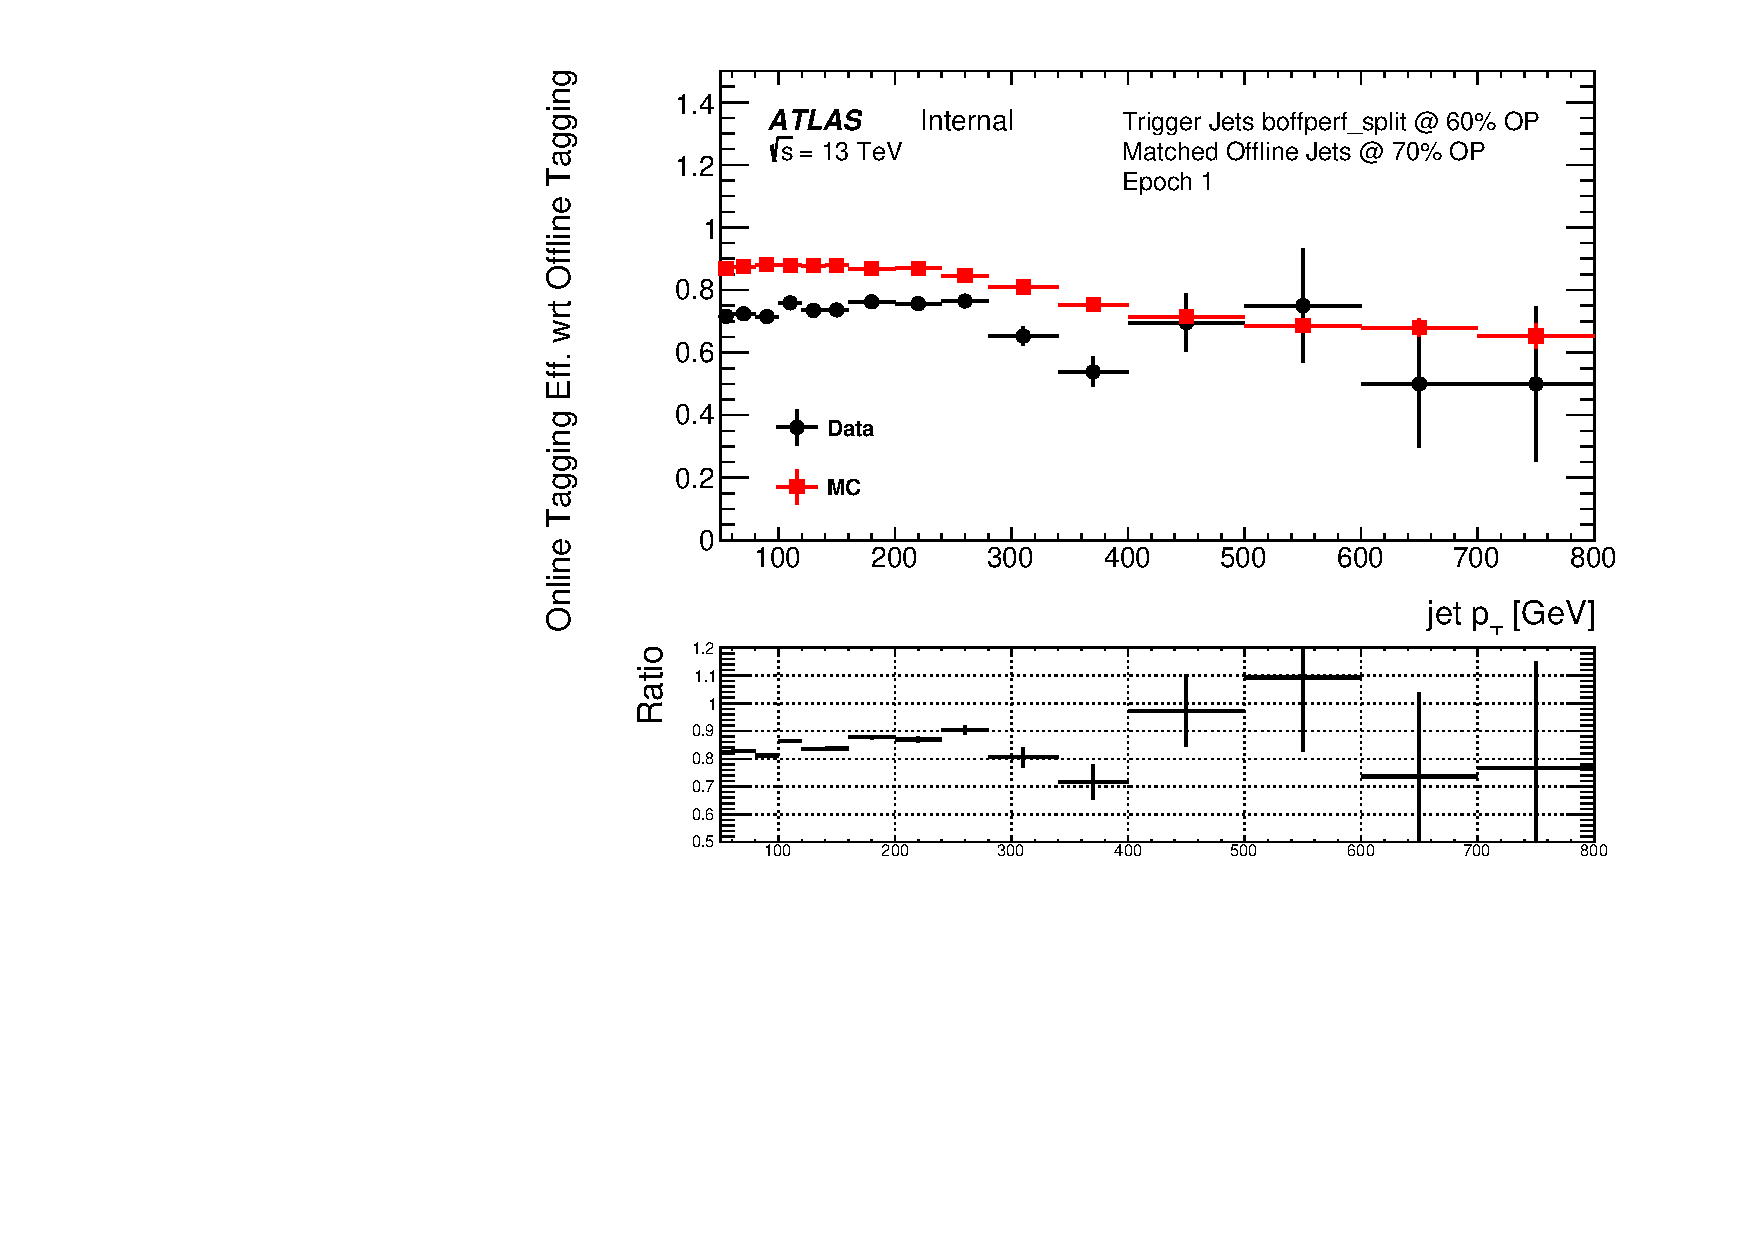
\includegraphics[width=0.48\linewidth, angle=0]{figs/Trigger/btrigger_old/Epoch1_trigReq_eff_jetPt.pdf} }
    \subcaptionbox{ $z_{bs}^{online}$}{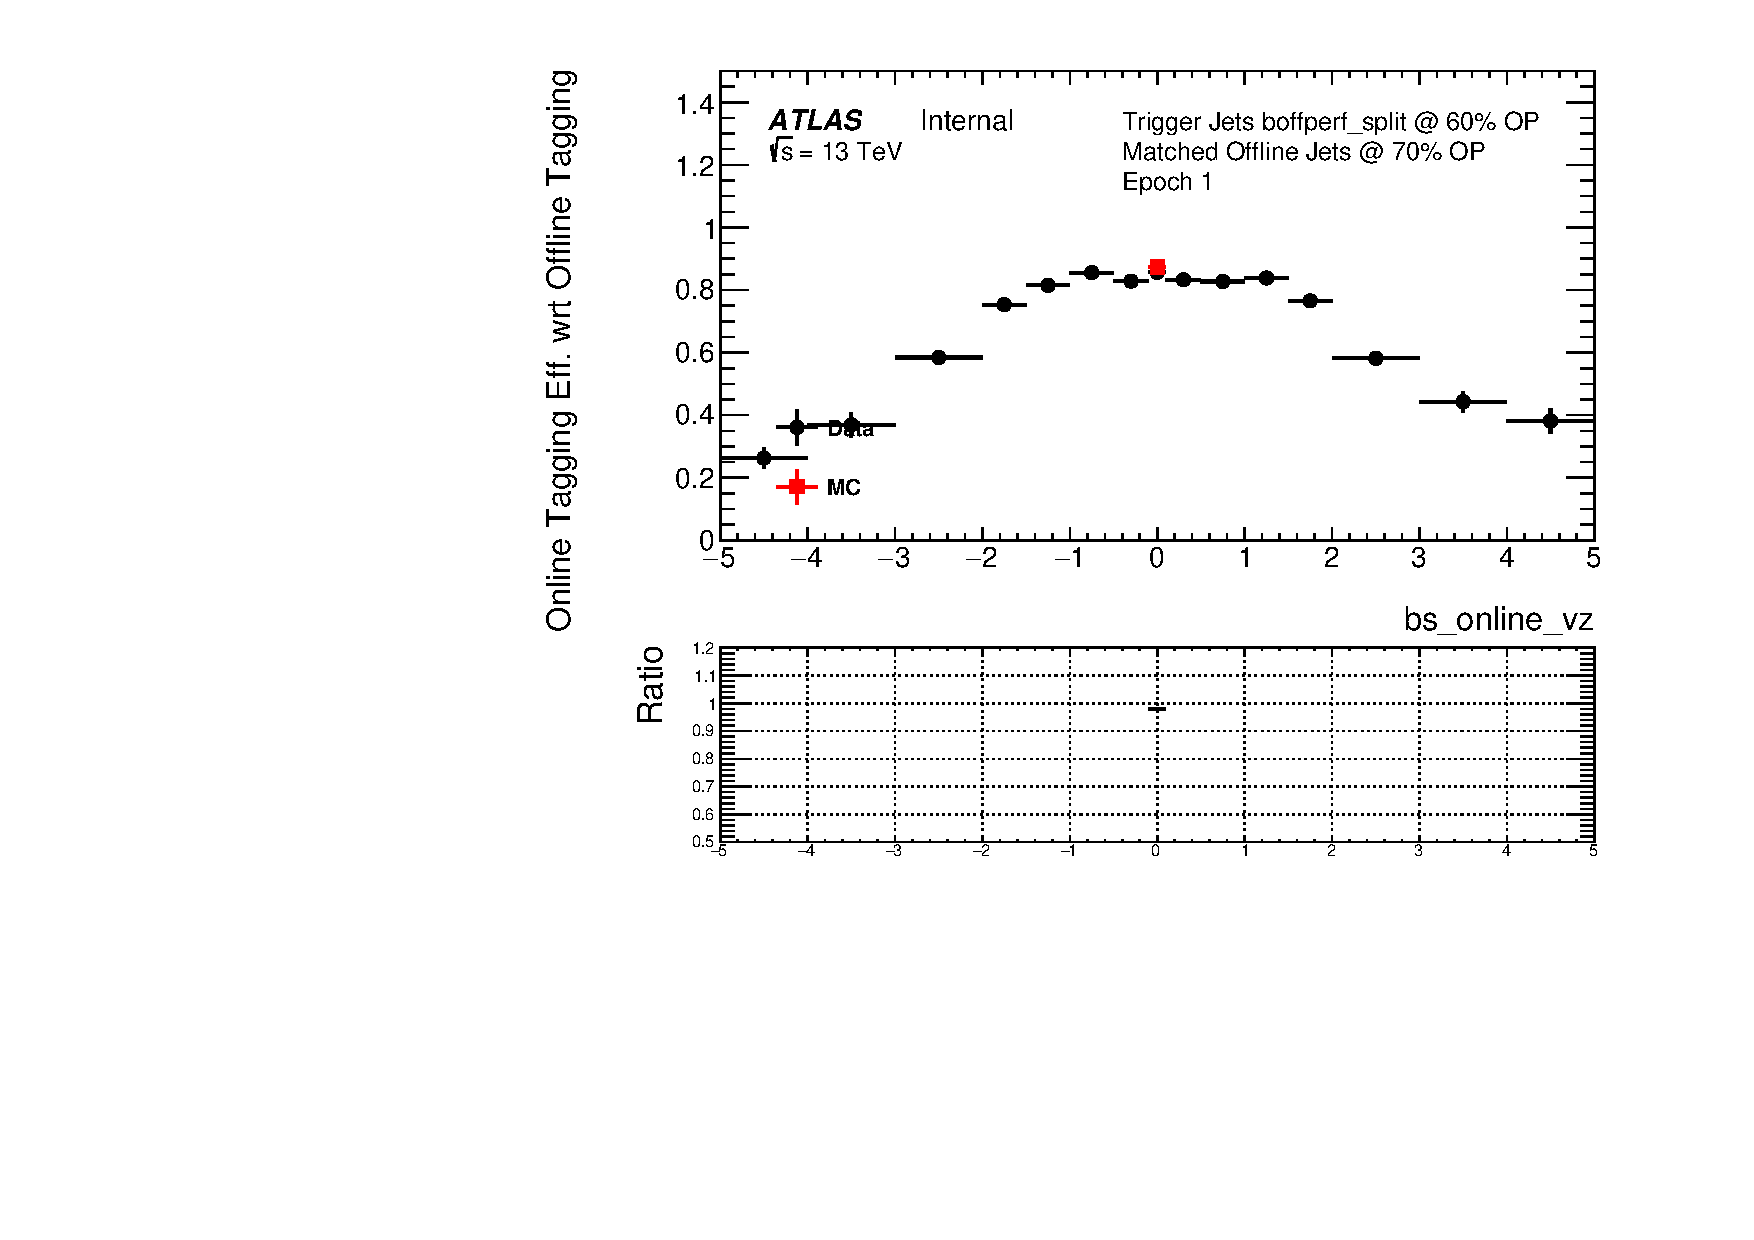
\includegraphics[width=0.48\linewidth, angle=0]{figs/Trigger/btrigger_old/Epoch1_trigReq_eff_bs_online_vz.pdf} }
  \end{center}
  \caption{The 60\% $b$-jet trigger efficiency with respect to an offline 70\% operating point tag
    for data from Epoch 1 (black) and simulation (red) against jet-\pT~(a) and online beamspot $z$-position (b).
    The $b$-jet trigger aware GRL has not been applied.}
  \label{fig:Epoch1_eff}
  \begin{center}
    \captionsetup[subfigure]{aboveskip=0pt,justification=centering}
    \subcaptionbox{$\epsilon_{bTrig}$ against Vertex Class}{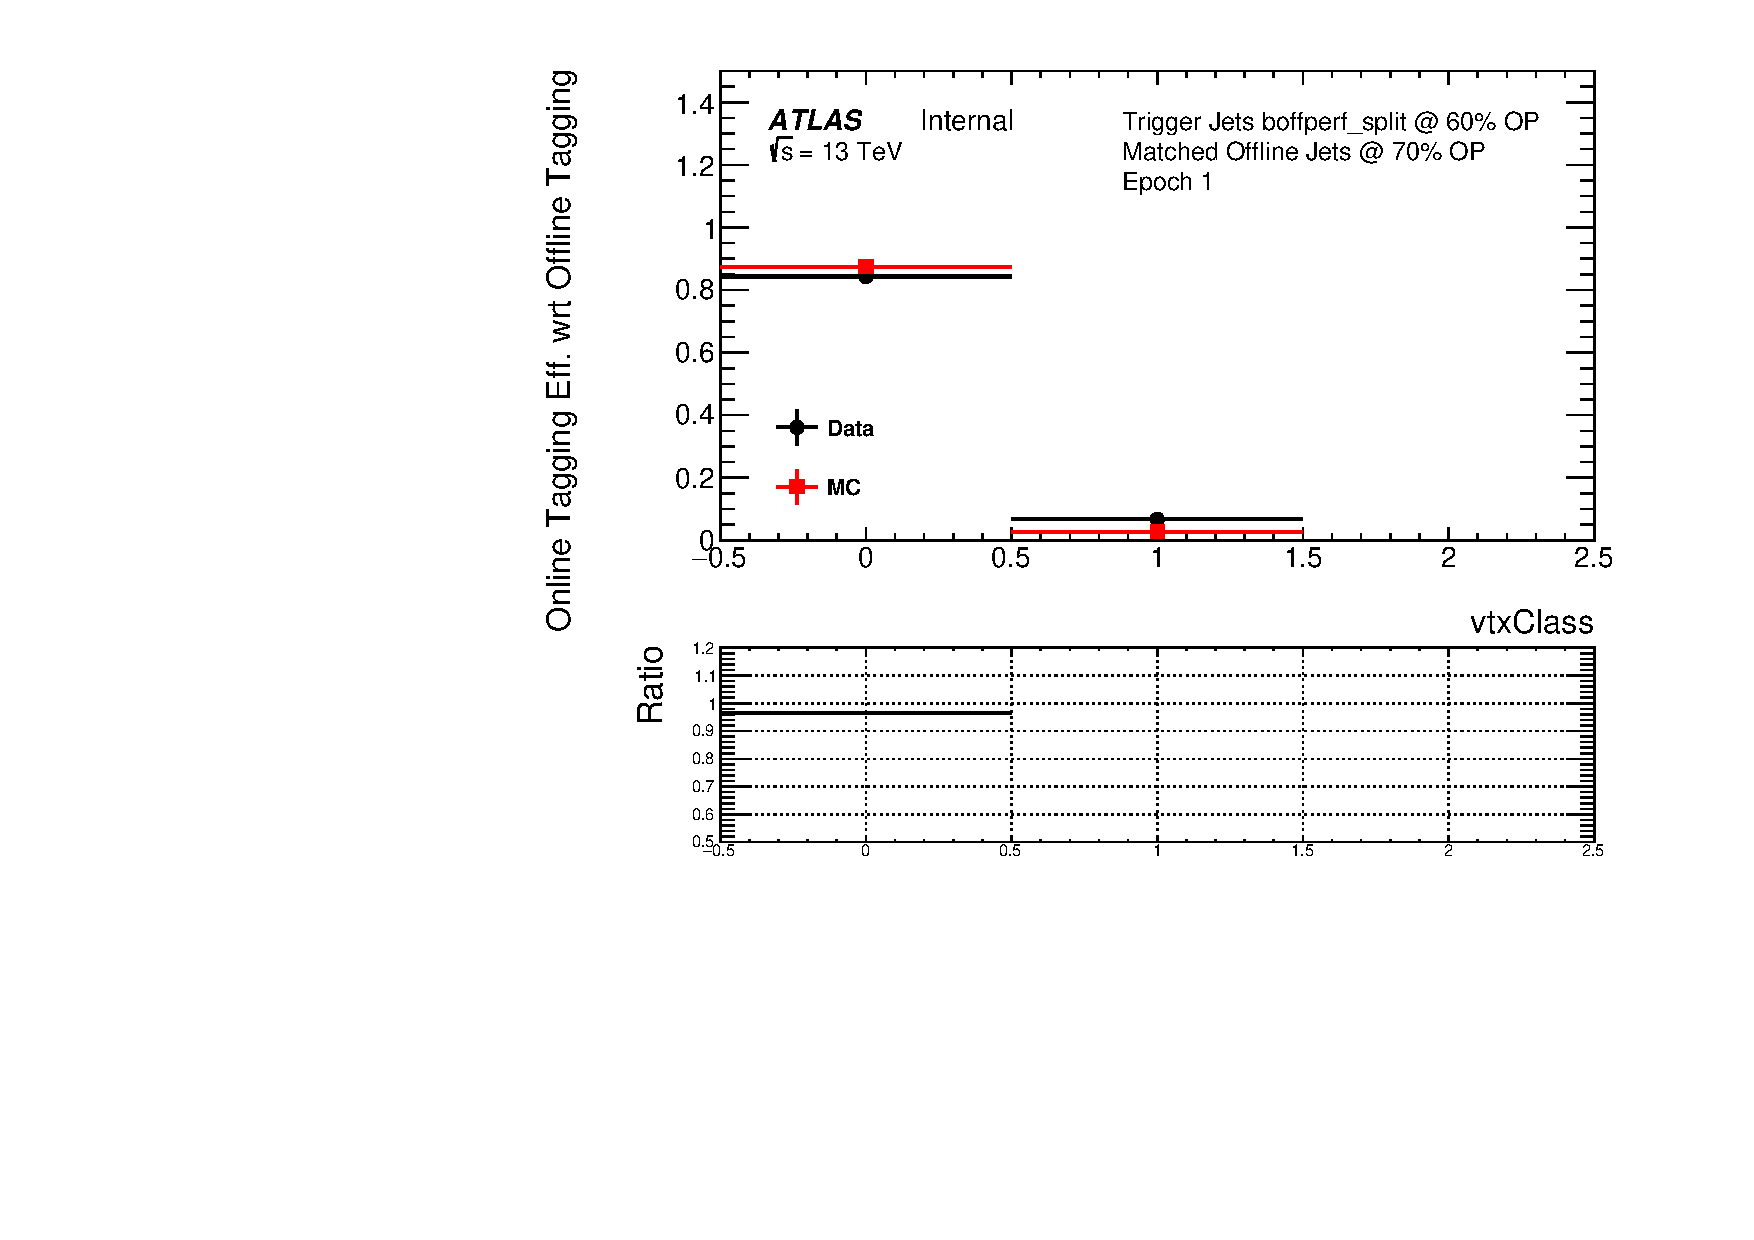
\includegraphics[width=0.48\linewidth, angle=0]{figs/Trigger/btrigger_old/Epoch1_trigReq_eff_vtxClass.pdf}}
    \subcaptionbox{Freq. of Offline Jets against Vertex Class}{\includegraphics[width=0.48\linewidth, angle=0]{figs/Trigger/btrigger_old/Epoch1_trigReq_nOff_vtxClass.pdf}}
    \end{center}
  \caption{(a) The 60\% $b$-jet trigger efficiency with respect to an offline 70\% operating point tag
    and  (b) the number of offline jets passing 70\% operating point tag and matching a HLT trigger jet
    against vertex class for data from Epoch 1 (black) and simulation (red). 
    The $b$-jet trigger aware GRL has not been applied.}
    \label{fig:Epoch1_vtxClass}
\end{figure}

\FloatBarrier


%\begin{figure}[!ht]
%\begin{center}
%  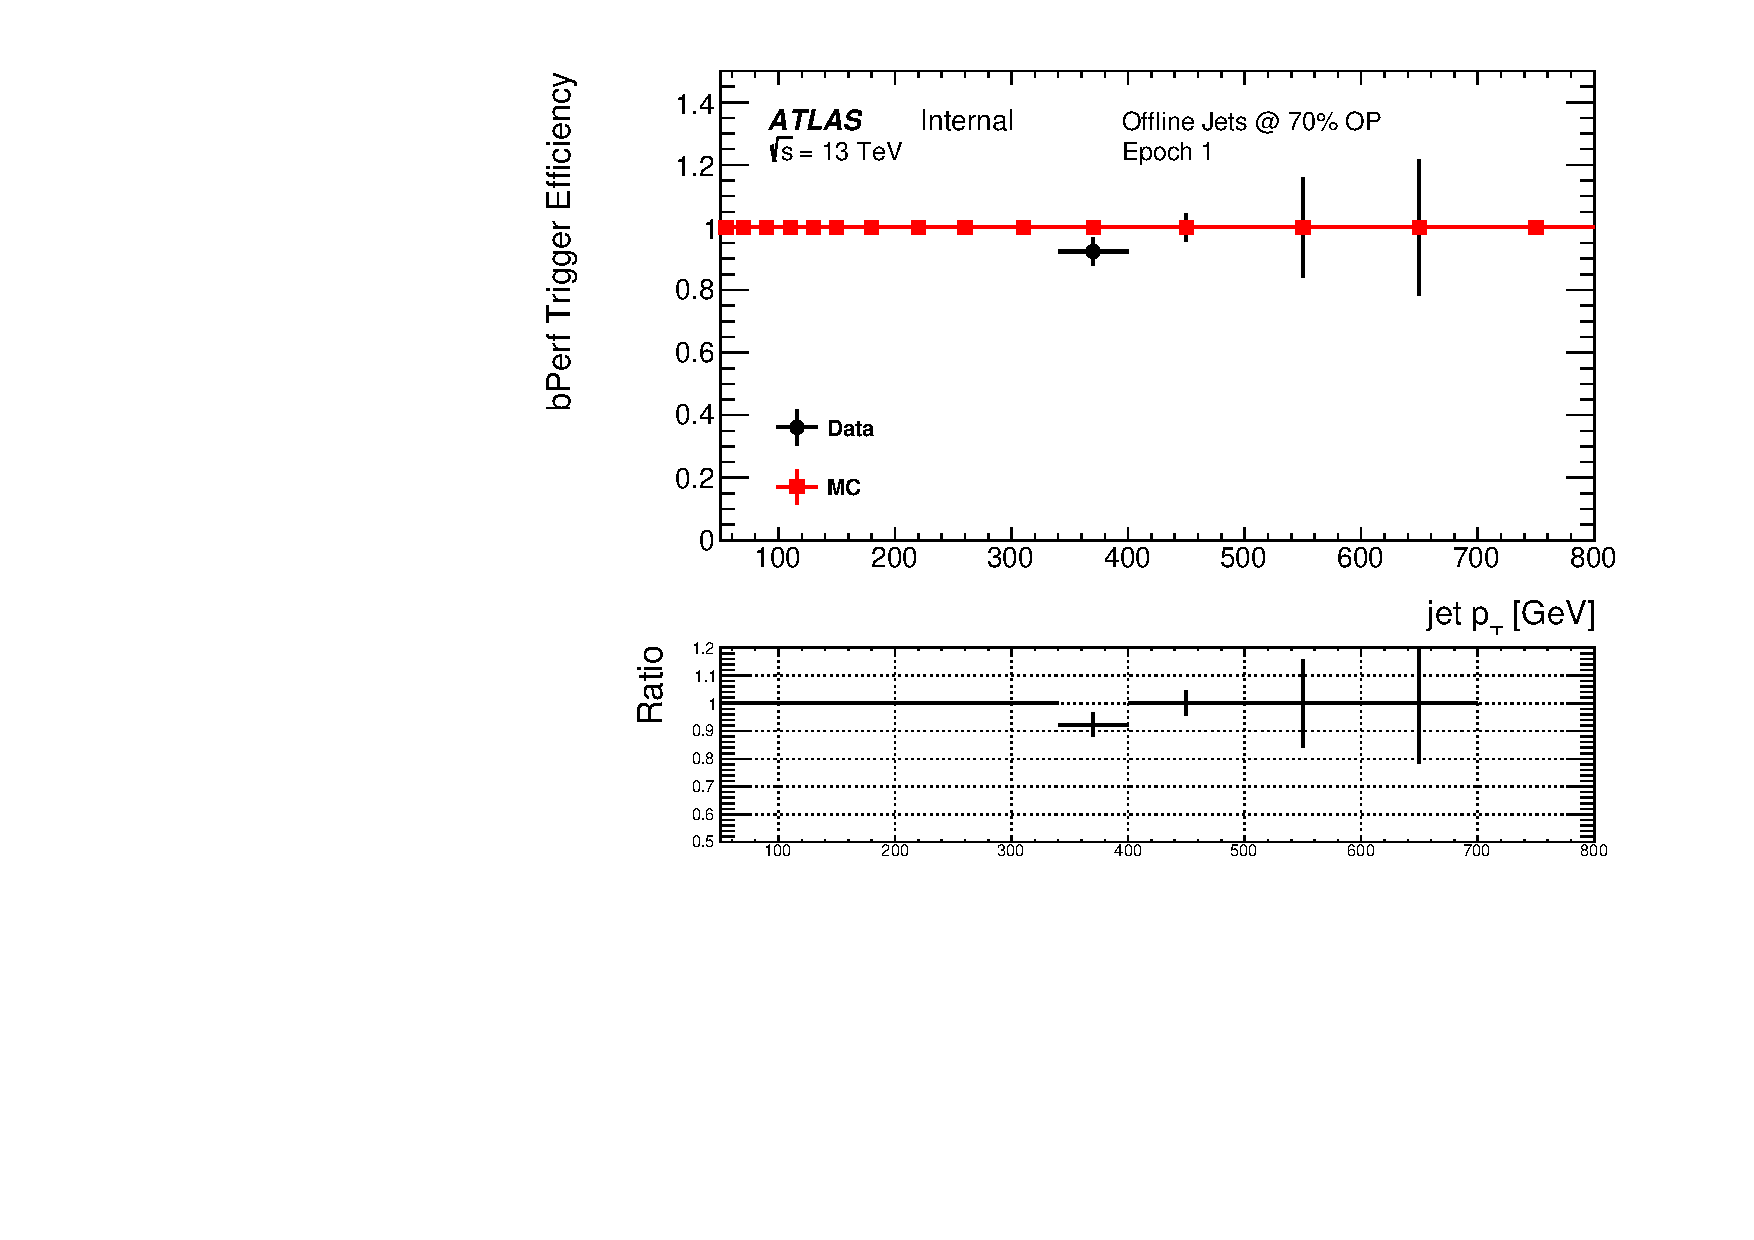
\includegraphics[width=0.47\linewidth, angle=0]{figs/Trigger/btrigger_old/Epoch1_trigReq_bPerfEff_jetPt.pdf}
%  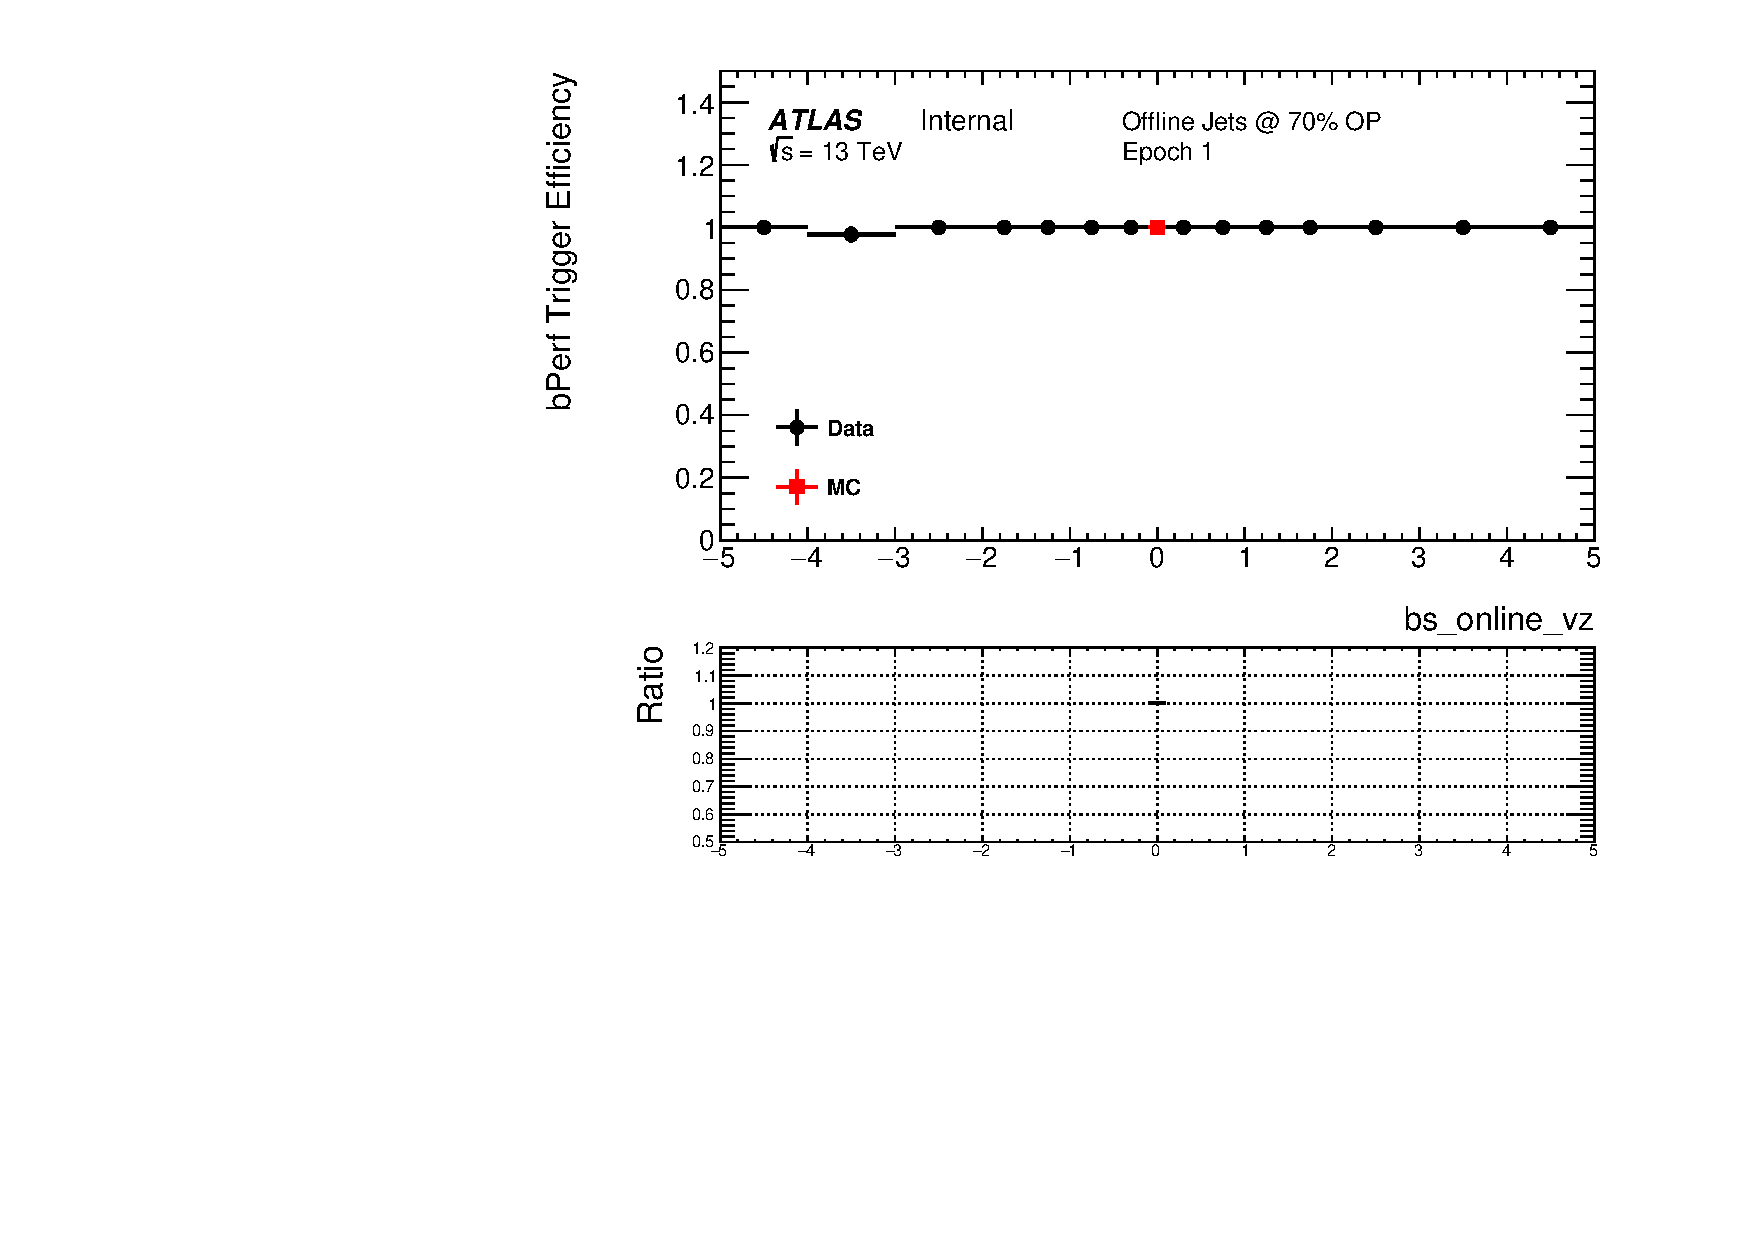
\includegraphics[width=0.47\linewidth, angle=0]{figs/Trigger/btrigger_old/Epoch1_trigReq_bPerfEff_bs_online_vz.pdf}
%\end{center}
%\caption{$b$-perf efficiency, $\epsilon_{bPerf}$, for data from Period A (black) and simulation (red) against jet-pT~(left) and online beamspot $z$-position (right).}
%\label{fig:Epoch1_bperf}
%\end{figure}

In Epoch 2, there is a similar problem to Epoch 1, but there is a subtle difference which requires us to look at this region in a
different way.
As in Epoch 1, when  $z_{bs}^{online}$ is far from zero then a \verb|xPrmVtx| PV is not found.
However in Epoch 2 this means that the  $b$-jet trigger was discovered to falsely terminate whilst processing the event,
meaning that there are no online $b$-jets are available in the event, and therefore the trigger will not fire.
However, the additional complication compared to Epoch 1 is this means that the  $b$-perf triggers used to measure the efficiency
are also not fired when no valid \verb|xPrmVtx| PV is available.
Hence, measuring $\epsilon_{bTrig}$ using the set-up as described will not capture the cases where a valid \verb|xPrmVtx| PV is found
and thus $\epsilon_{bTrig}$ should be consistent in data and simulation;
Figure~\ref{fig:Epoch2_eff} shows that the $\epsilon_{bTrig}$ measured in data to be in agreement with simulation within 5\%.


For Epoch 2, in addition to measuring $\epsilon_{bTrig}$ it is necessary
to also account for the cases when a false \verb|xPrmVtx| PV is found.
This is done by measuring the $b$-perf efficiency, $\epsilon_{bPerf}$,
the efficiency that there is a valid primary vertex in the event.
$\epsilon_{bPerf}$ is calculated by dividing the number of events that pass the trigger
\verb|HLT_mu26_imedium_2j35_bperf| by the number that pass the trigger \verb|HLT_mu26_imedium|,
such that the denominator has no $b$-trigger dependency so is unaffected by \verb|xPrmVtx| PV.
This is an event level quantity and as such is measured with respect to other event level quantities, such as leading jet-\pT.
Figure~\ref{fig:Epoch2_bperf} shows that:
$\epsilon_{bPerf}$ has a data/simulation ratio of around 80\%  which is similar to that in Section~\ref{sec:trig-initProb} and
$\epsilon_{bPerf}$ shows similar behaviour with respect to  $z_{bs}^{online}$ as observed in Epoch 1.
Finally it is observed that $\epsilon_{bPerf}$ has a lower efficiency at smaller values of absolute leading jet-$\eta$;
this is due to the fact that at high-$\eta$ tracks have a larger error on the longitudinal impact parameter, $z_0$,
meaning that the mis-match of co-ordinates can in the \verb|xPrmVtx| algorithm is covered by the errors, mitigating this issue.
This effect must be accounted for in the final efficiency measurement.\textbf{This last two sentances are dodgy}

\begin{figure}[!ht]
\begin{center}
  \captionsetup[subfigure]{aboveskip=0pt,justification=centering}
  \subcaptionbox{Jet-\pT}{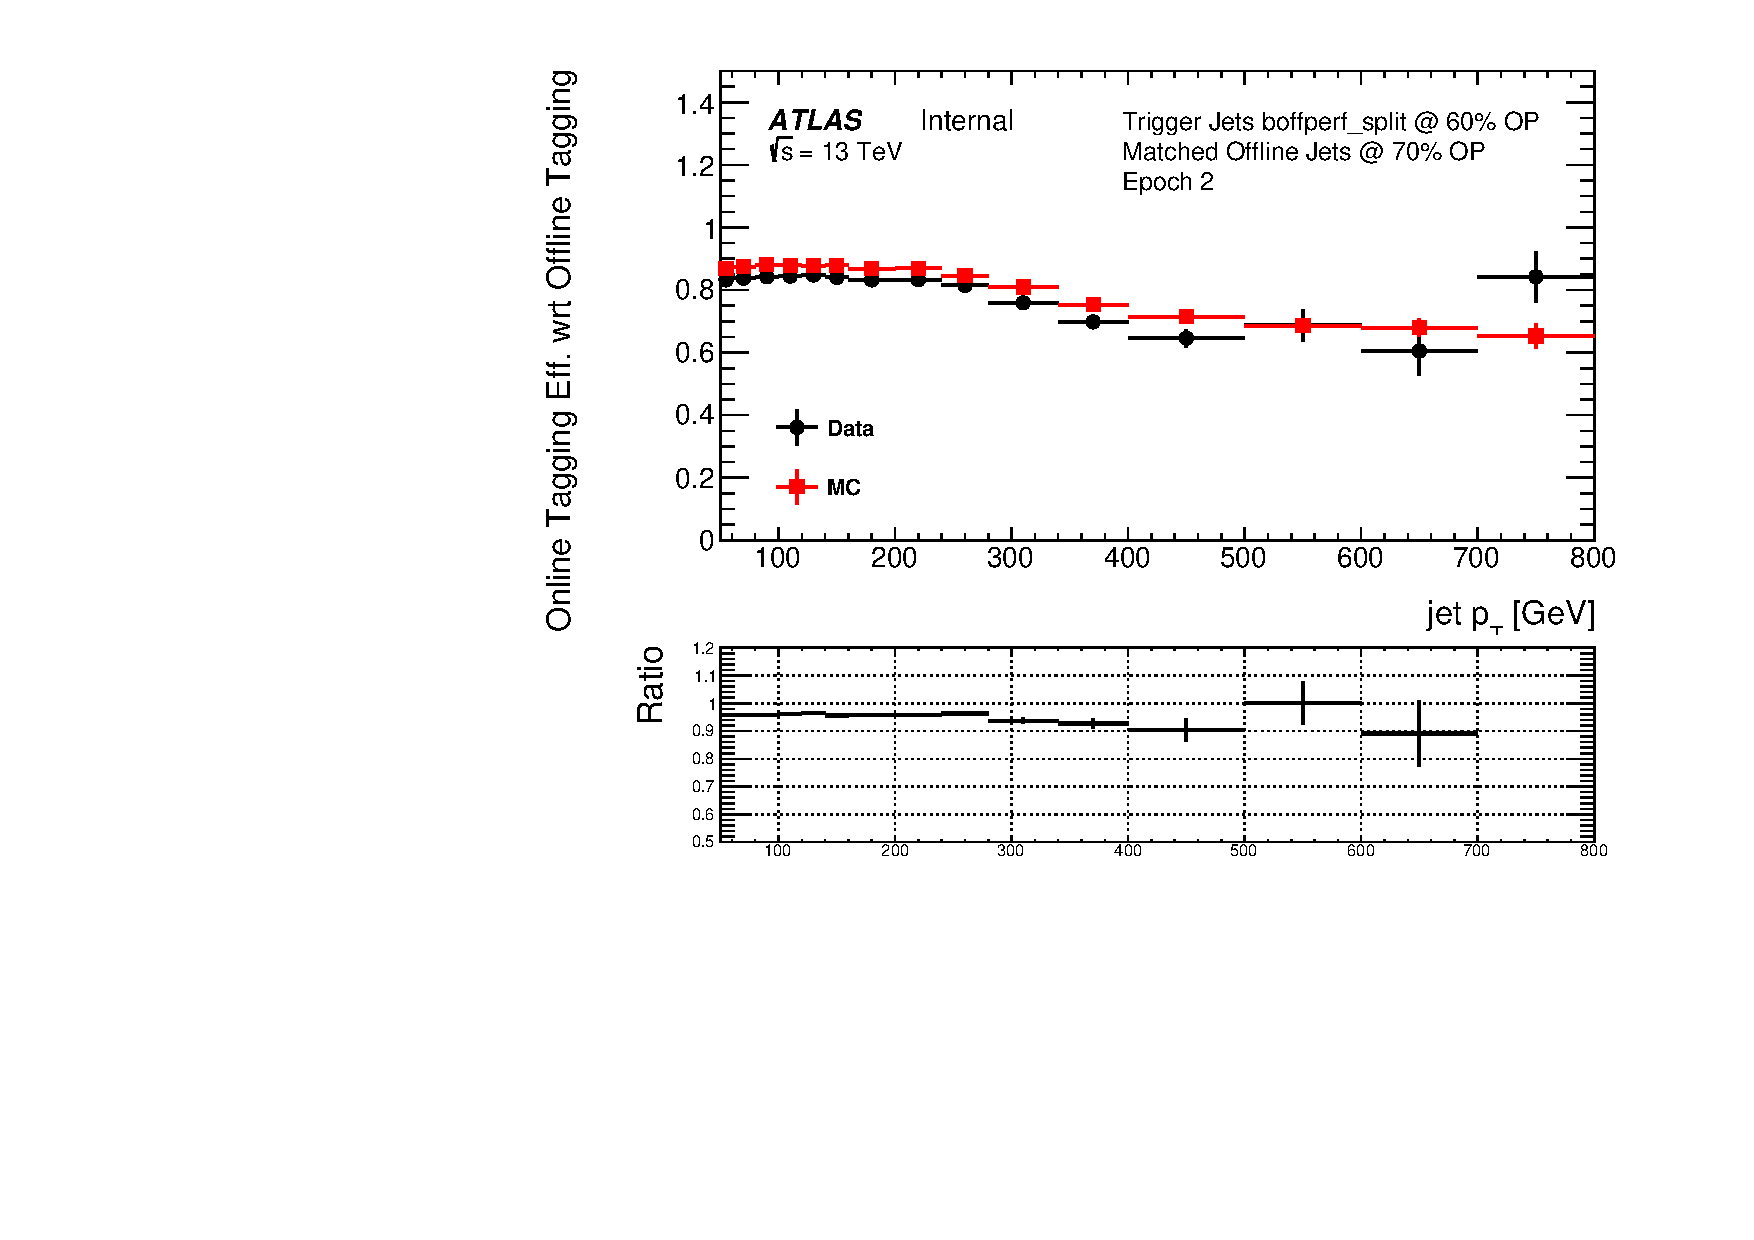
\includegraphics[width=0.47\linewidth, angle=0]{figs/Trigger/btrigger_old/Epoch2_trigReq_eff_jetPt.pdf}}     
  \subcaptionbox{Jet-$\eta$}{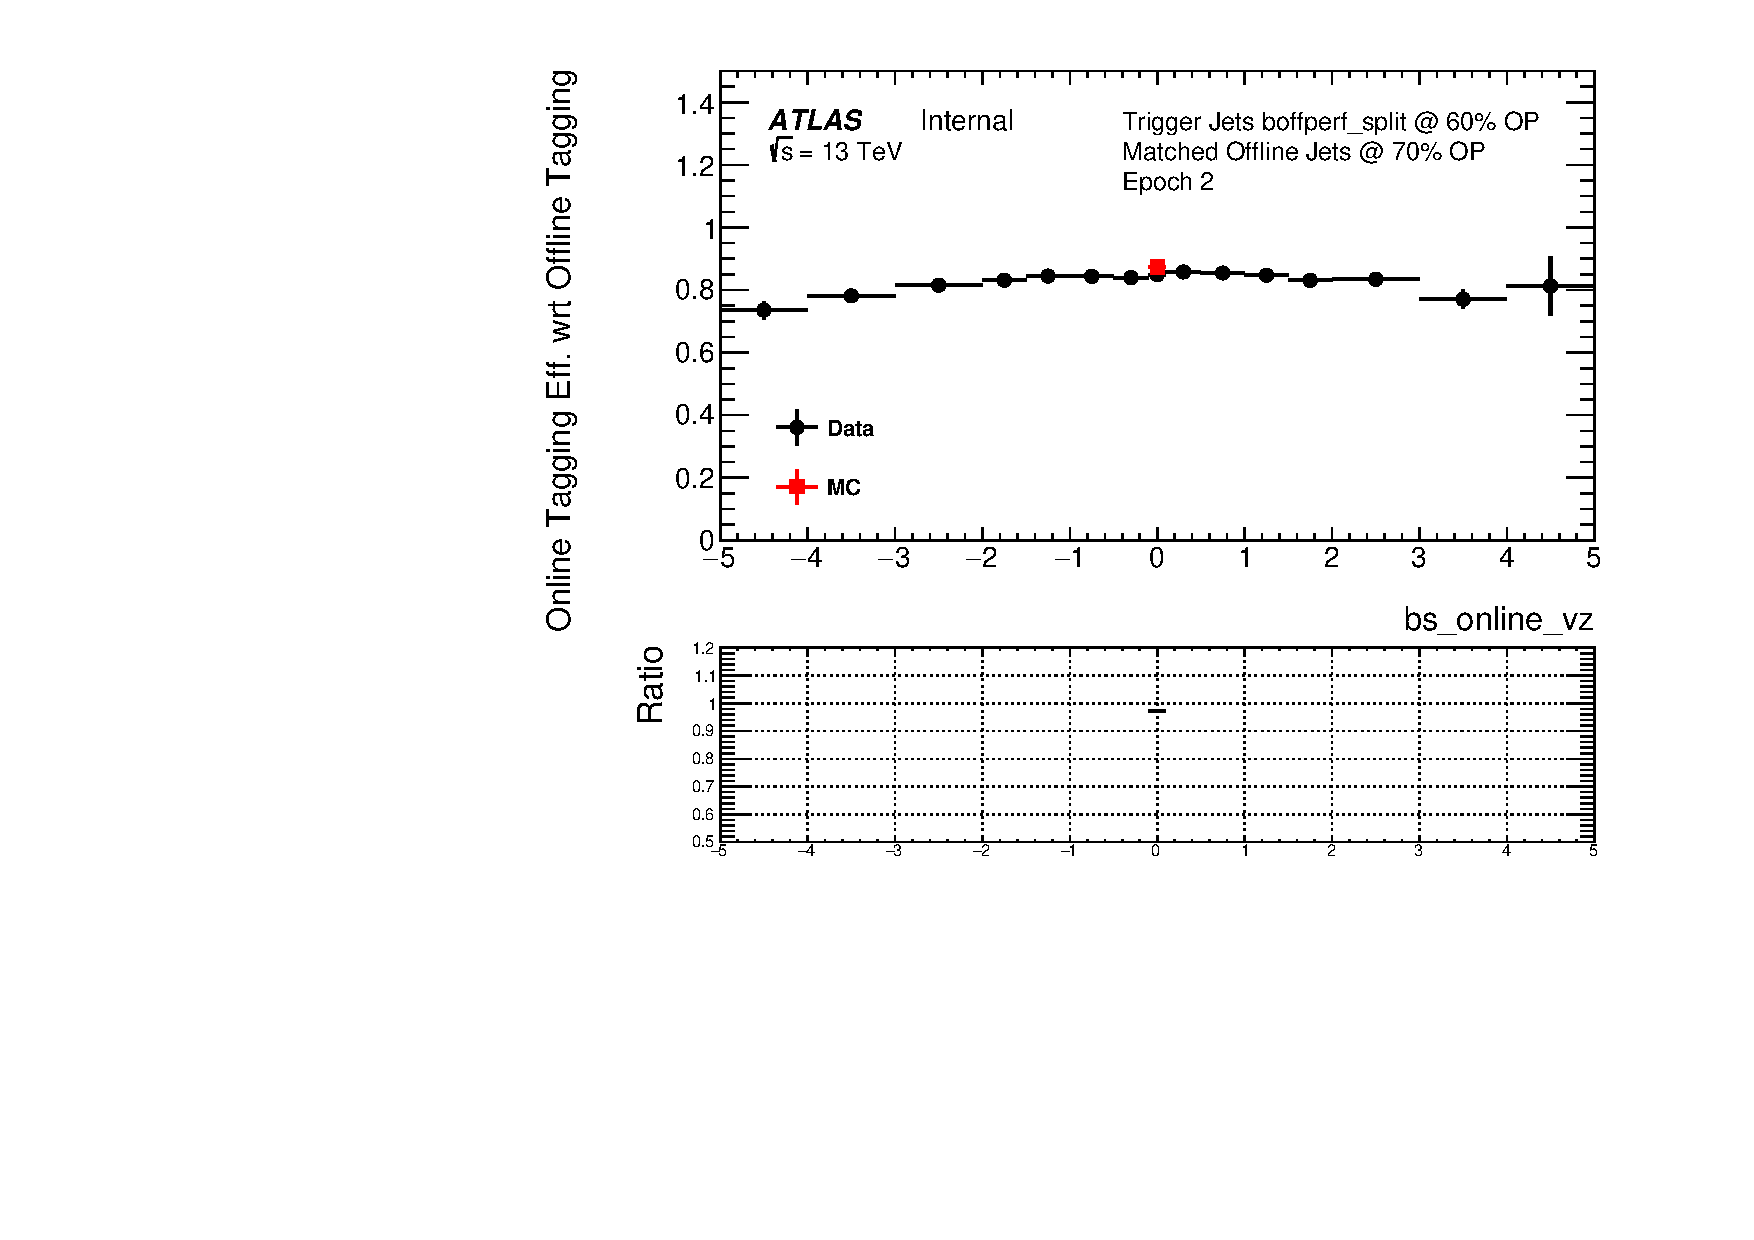
\includegraphics[width=0.47\linewidth, angle=0]{figs/Trigger/btrigger_old/Epoch2_trigReq_eff_bs_online_vz.pdf}}
  %\subcaptionbox{??}{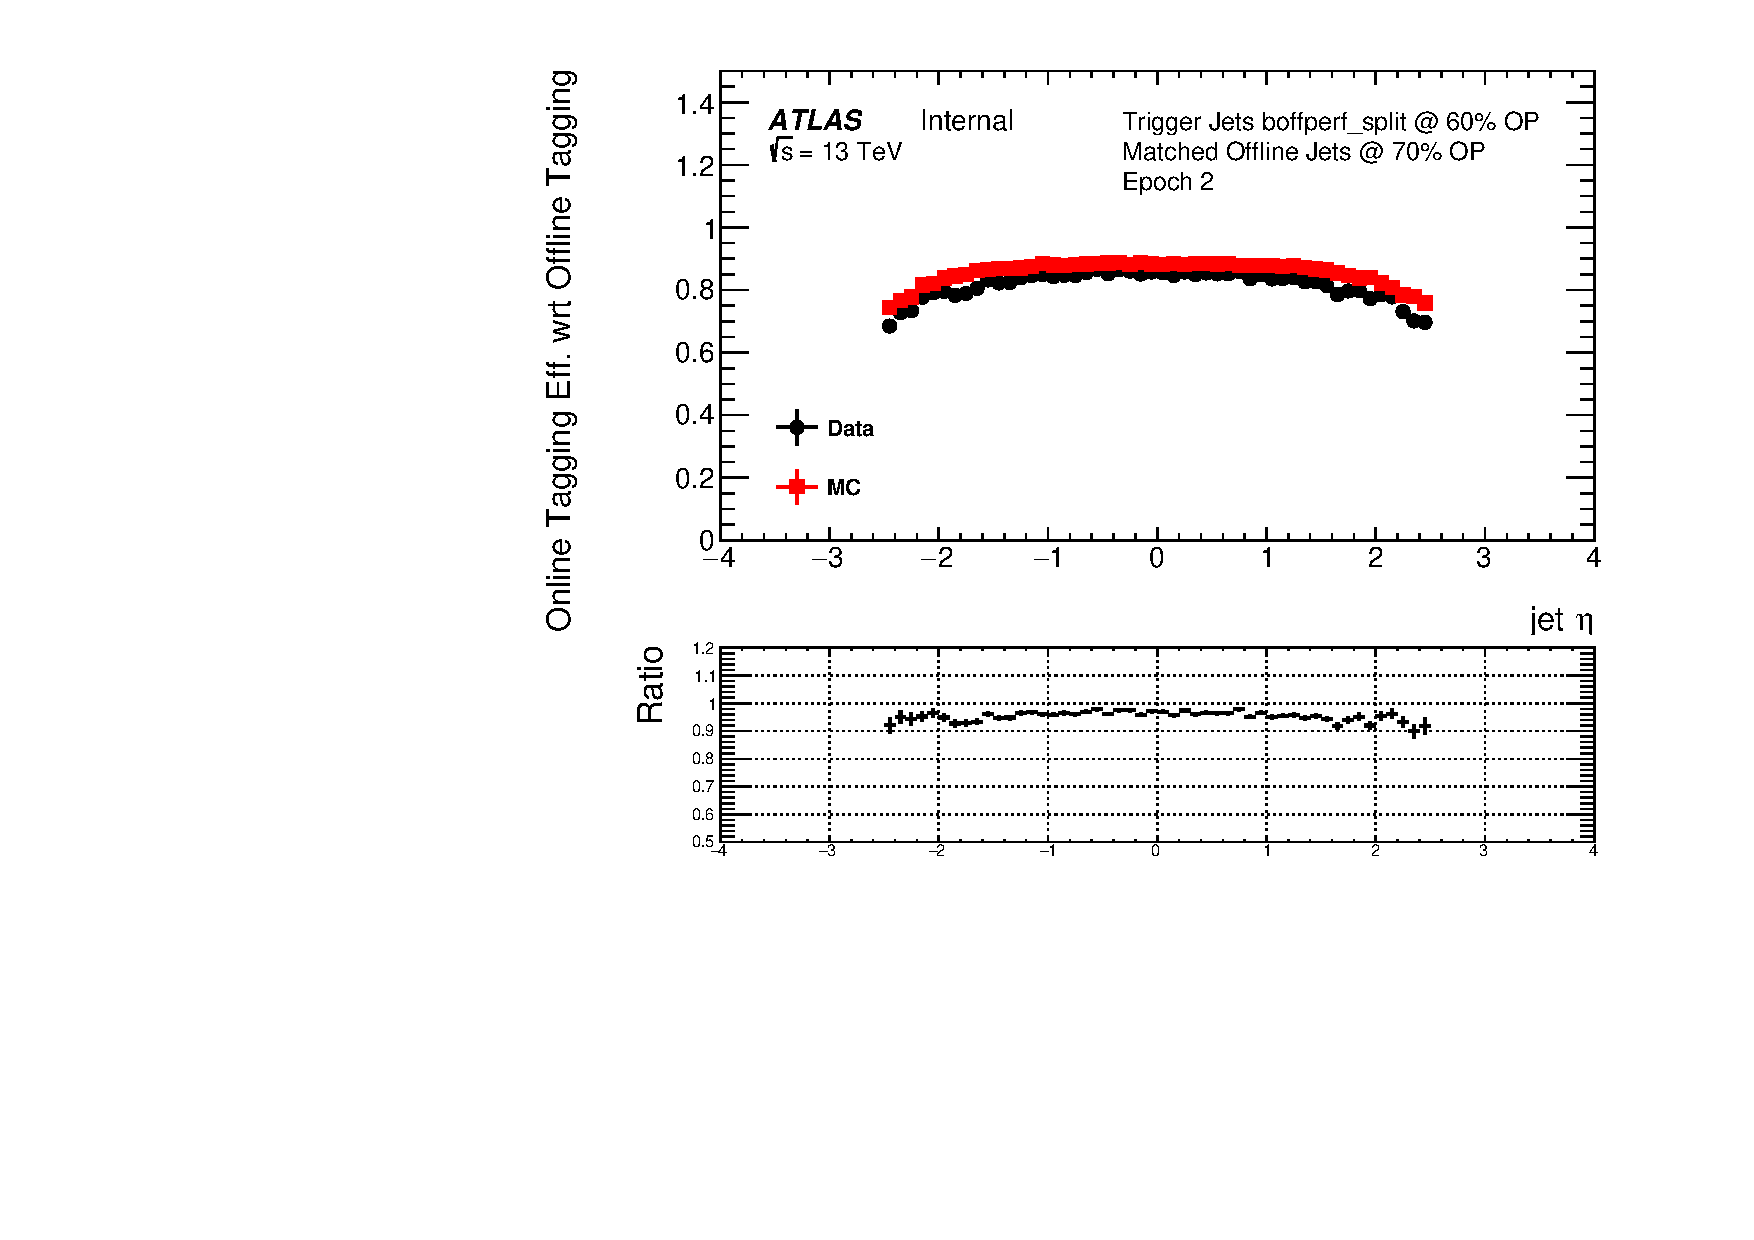
\includegraphics[width=0.47\linewidth, angle=0]{figs/Trigger/btrigger_old/Epoch2_trigReq_eff_jetEta.pdf}} \\
  %\subcaptionbox{??}{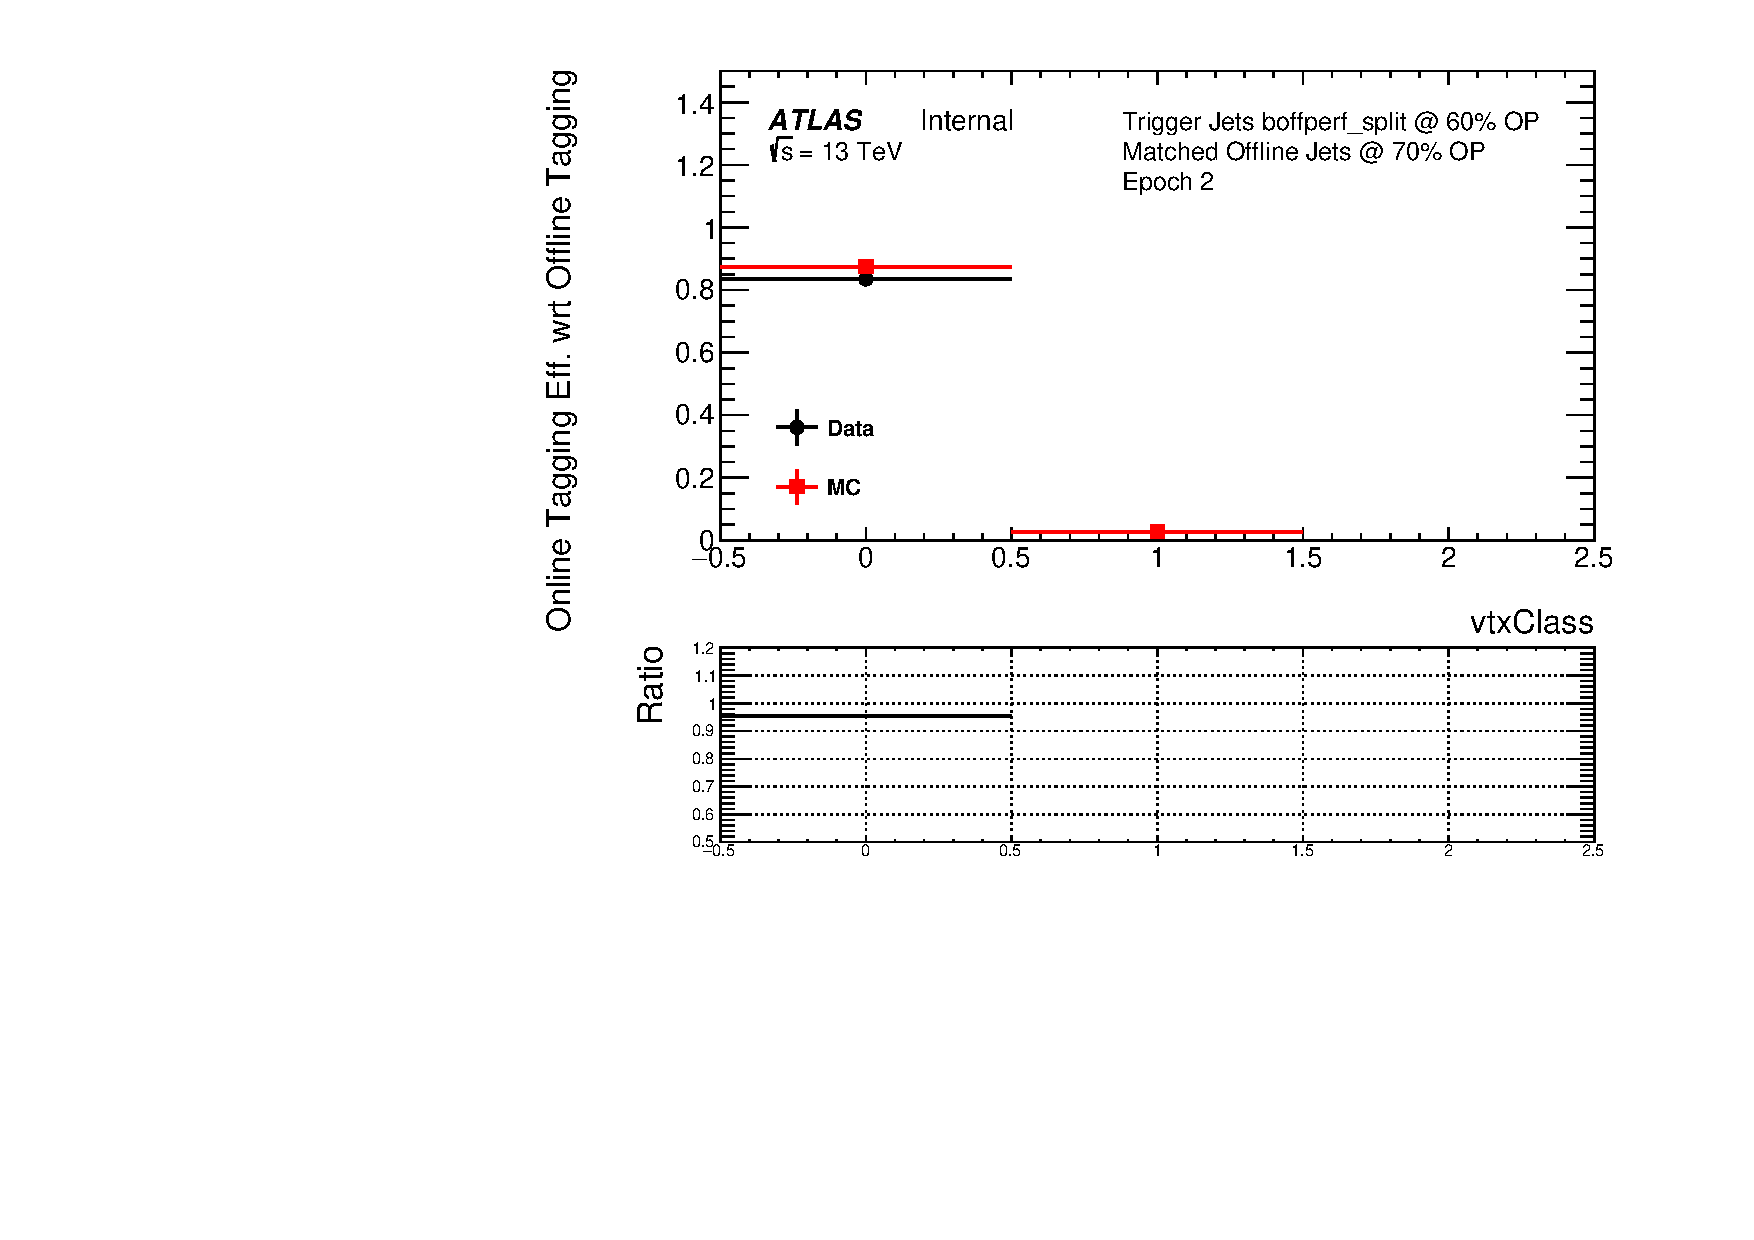
\includegraphics[width=0.47\linewidth, angle=0]{figs/Trigger/btrigger_old/Epoch2_trigReq_eff_vtxClass.pdf}}
\end{center}
\caption{The 60\% $b$-jet trigger efficiency with respect to an offline 70\% operating point tag
         for data from epoch 2 (black) and simulation (red) against jet-\pT~(a), jet-$\eta$ (b) and online beamspot $z$-position (c).}
\label{fig:Epoch2_eff}
\begin{center}
  \captionsetup[subfigure]{aboveskip=0pt,justification=centering}
  \subcaptionbox{Leading Jet-\pT}{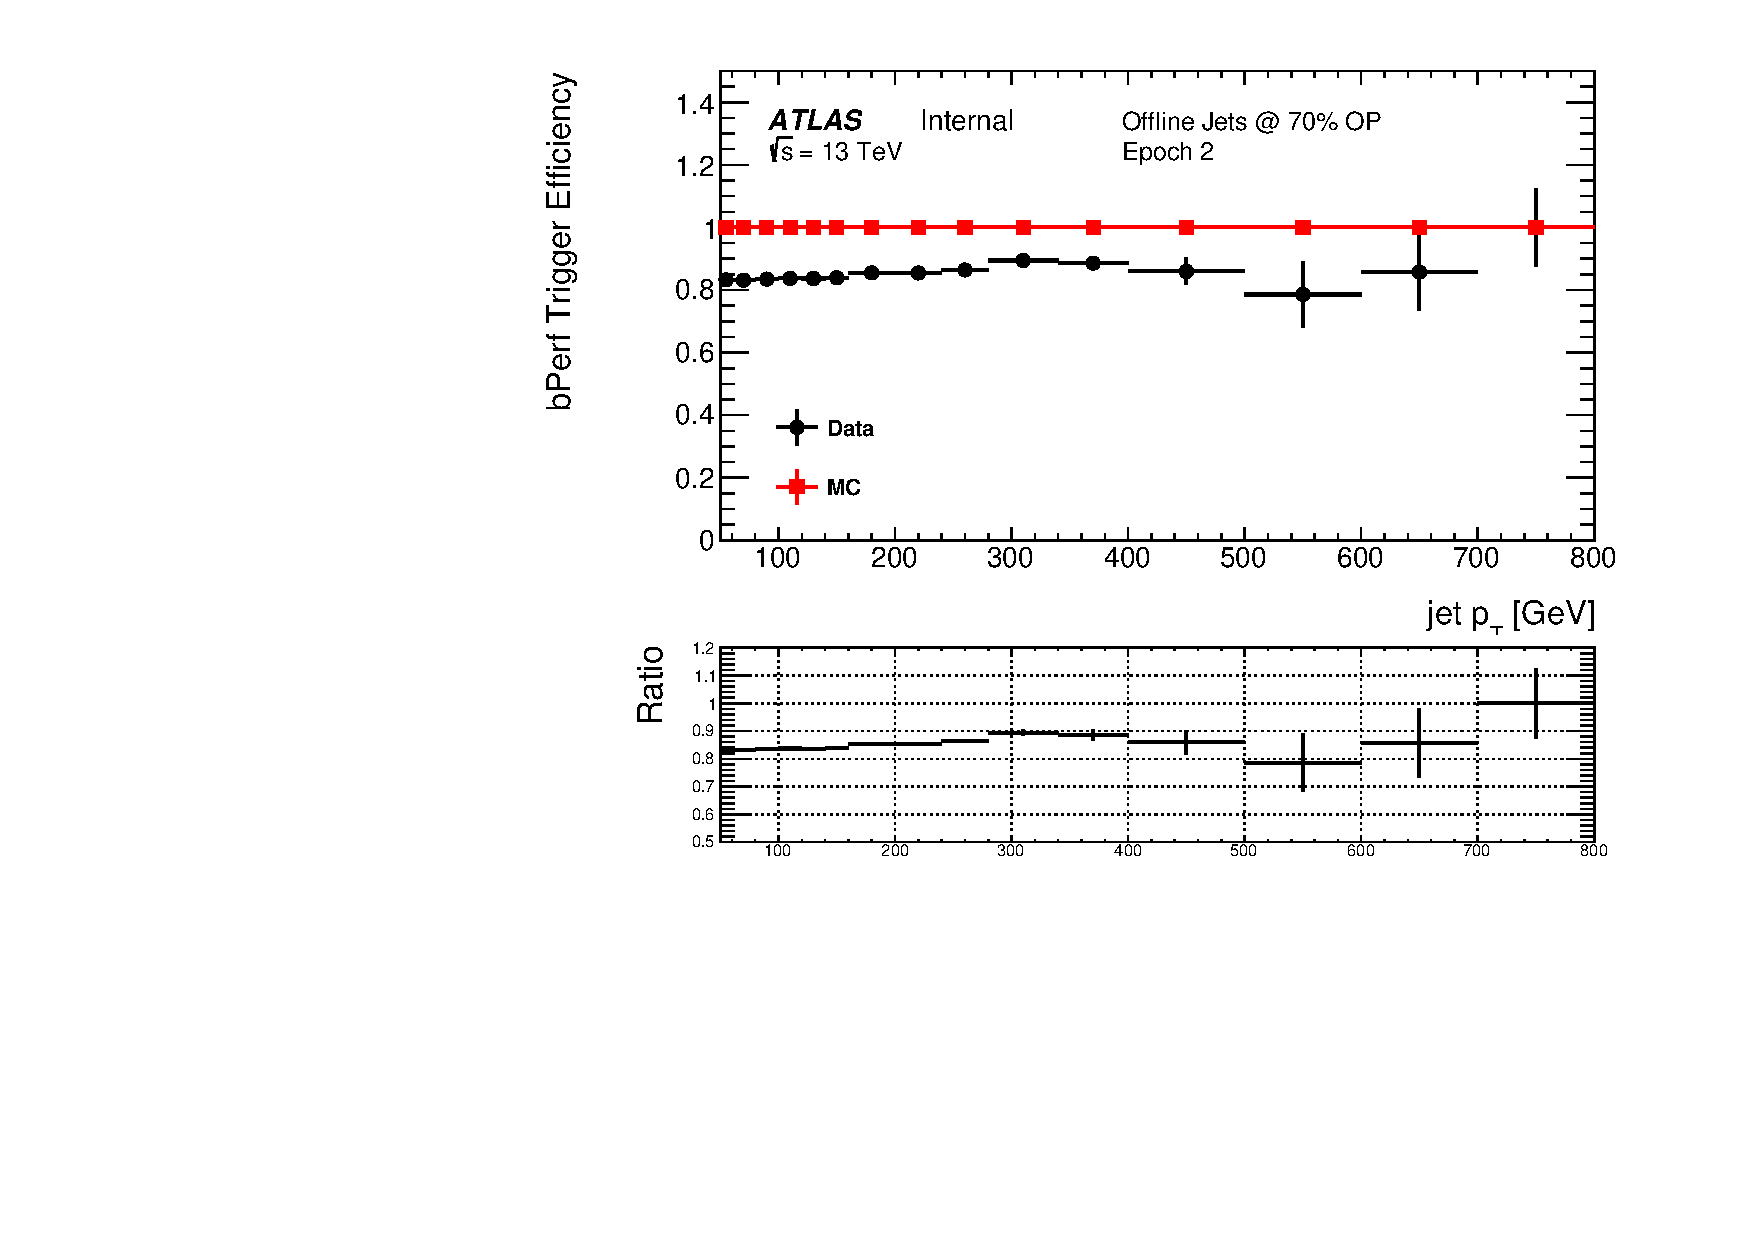
\includegraphics[width=0.47\linewidth, angle=0]{figs/Trigger/btrigger_old/Epoch2_trigReq_bPerfEff_jetPt.pdf}}
  \subcaptionbox{$z_{bs}^{online}$}{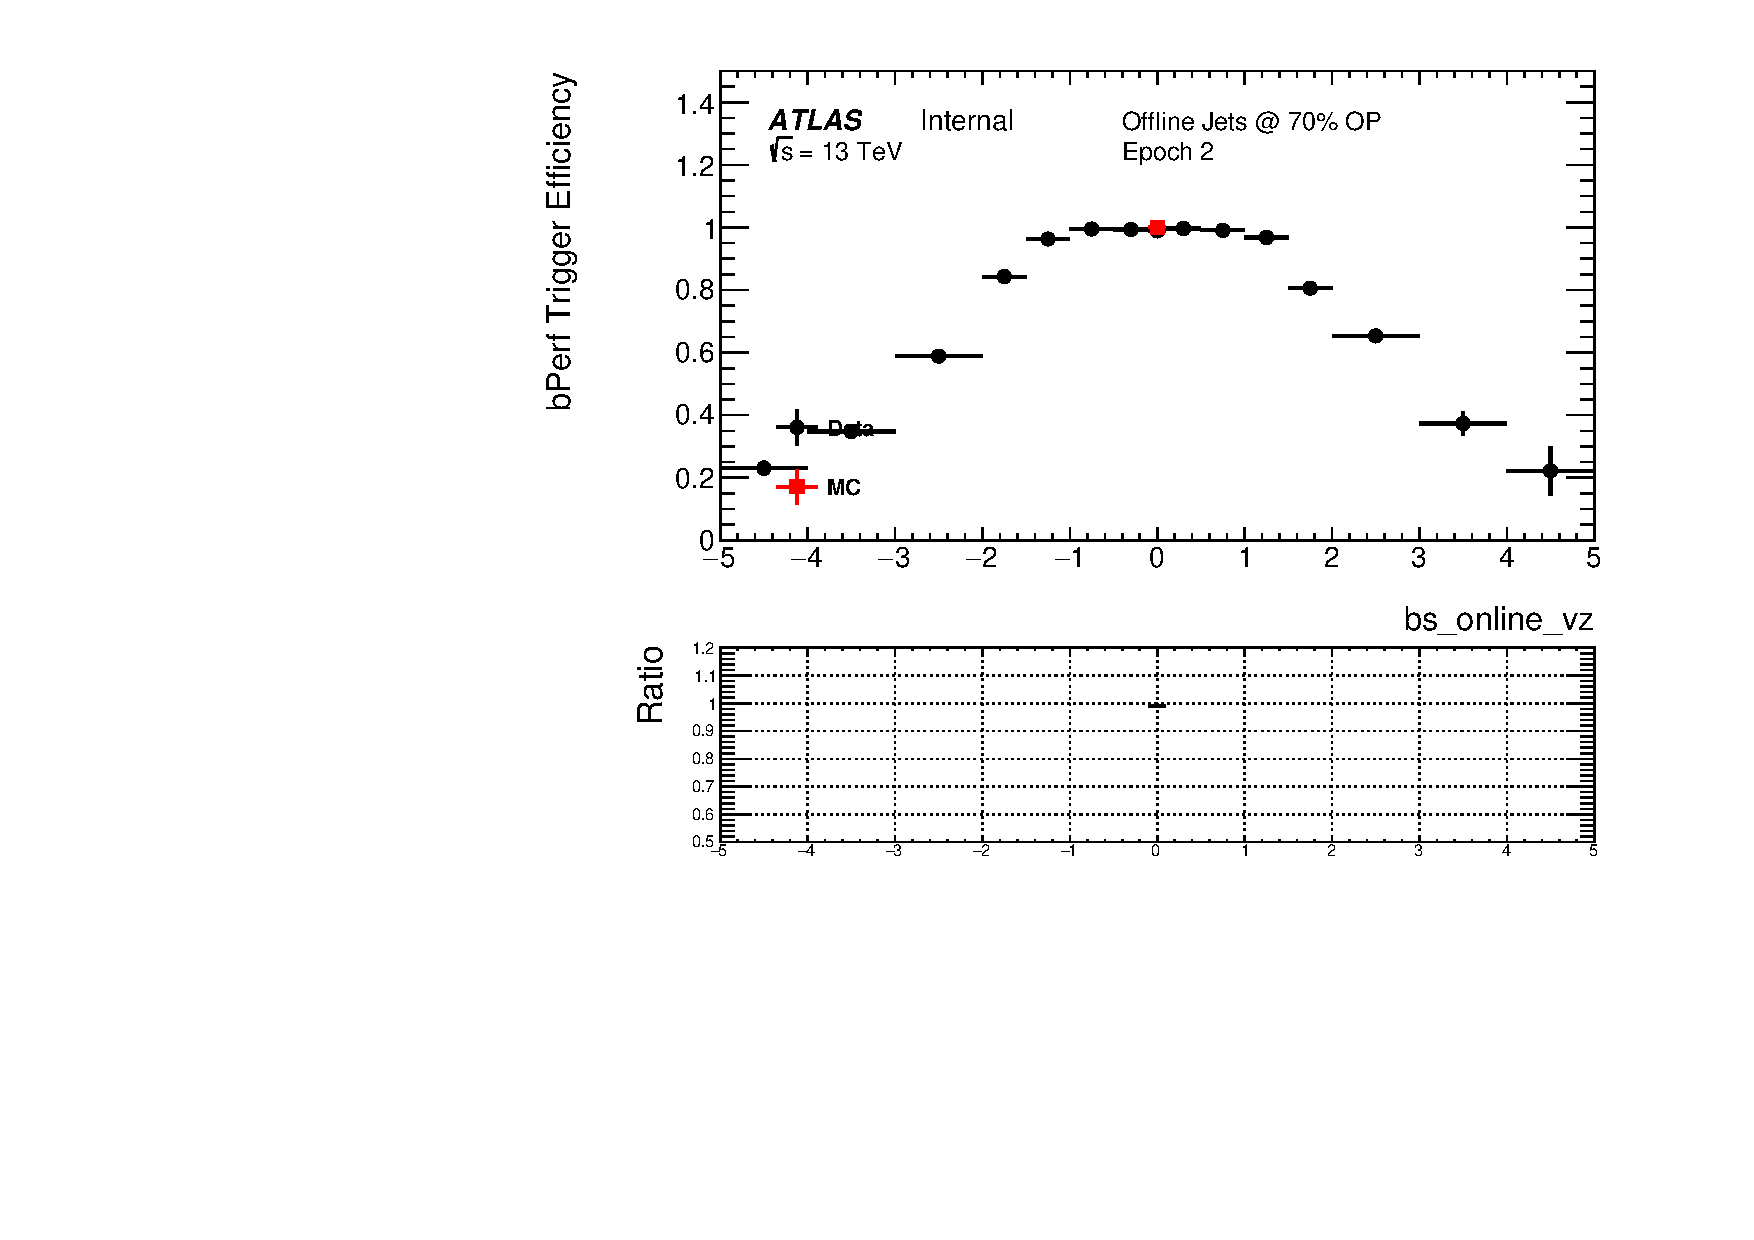
\includegraphics[width=0.47\linewidth, angle=0]{figs/Trigger/btrigger_old/Epoch2_trigReq_bPerfEff_bs_online_vz.pdf}}
  \subcaptionbox{Leading Jet-$\eta$}{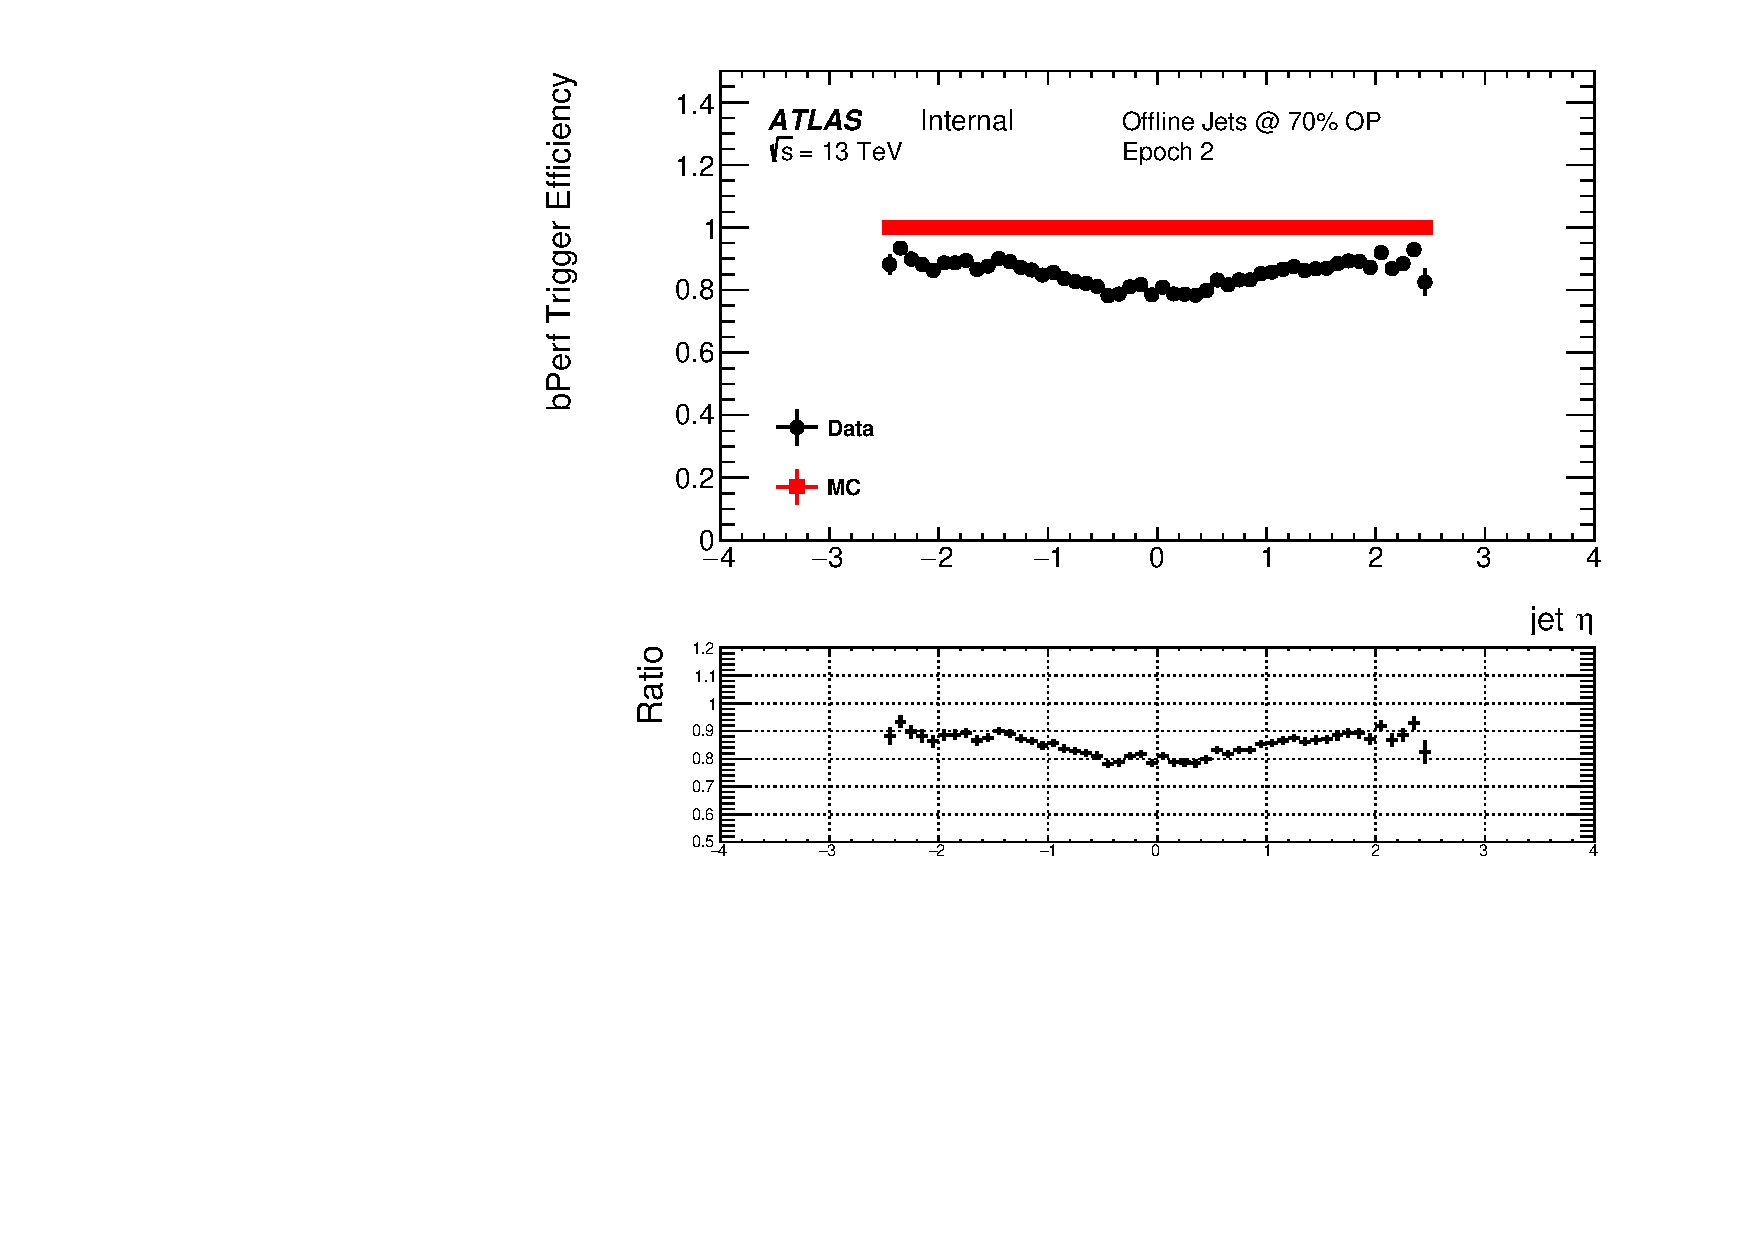
\includegraphics[width=0.47\linewidth, angle=0]{figs/Trigger/btrigger_old/Epoch2_trigReq_bPerfEff_jetEta.pdf}}
\end{center}
\caption{$b$-perf efficiency, $\epsilon_{bPerf}$, for data from Epoch 2 (black) and simulation (red) against leading-jet \pT~(a), online beamspot $z$-position (b) and leading jet-$\eta$ (c).}
\label{fig:Epoch2_bperf}
\end{figure}
Epoch 3, when no \verb|xPrmVtx| PV is found then a backup PV finding algorithm is used, known as \verb|EFHist|, which finds the PV through a basic histogramming of the tracks,
the simplicity of the algorithm means that a PV can be found as long as 1 track is present.
Figure~\ref{fig:Epoch3_eff} shows $\epsilon_{bTrig}$ for Epoch 3 for jet-\pT, jet-$\eta$,  $z_{bs}^{online}$ and vertex class (as defined above).
In Epoch 3 $\epsilon_{bTrig}$ measured in data is within 5\% of simulation and there is no shape difference between the two with respect to jet-$\eta$.
In addition it is shown that in Epoch 3 there is no strong dependence on  $z_{bs}^{online}$,
and that efficiency in data is consistent if a valid \verb|xPrmVtx| vertex or not (vertex class = 0 or 1 respectively).
This demonstrates the success of the backup vertex approach.

\begin{figure}[!ht]
\begin{center}
  \captionsetup[subfigure]{aboveskip=0pt,justification=centering}
  \subcaptionbox{Jet-\pT}{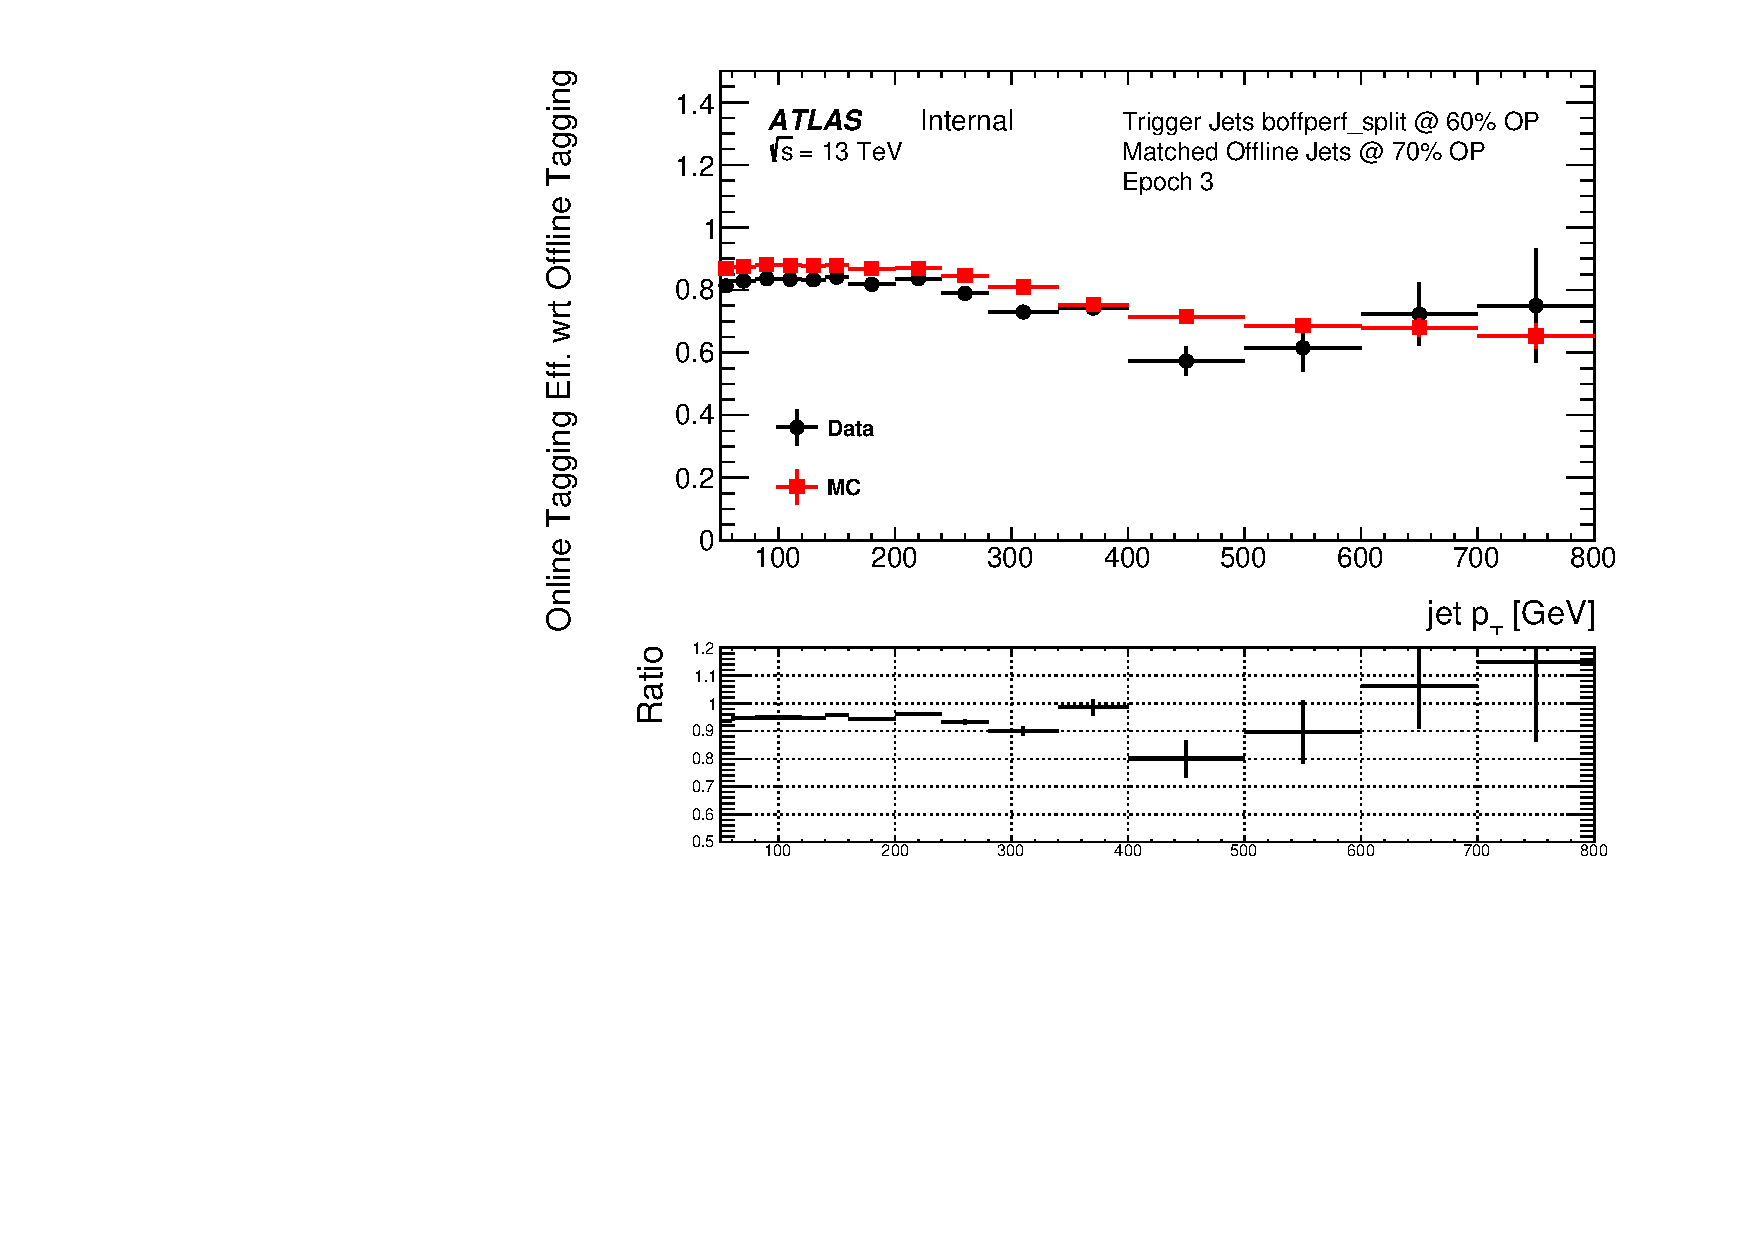
\includegraphics[width=0.47\linewidth, angle=0]{figs/Trigger/btrigger_old/Epoch3_trigReq_eff_jetPt.pdf}}
  \subcaptionbox{Jet-$\eta$}{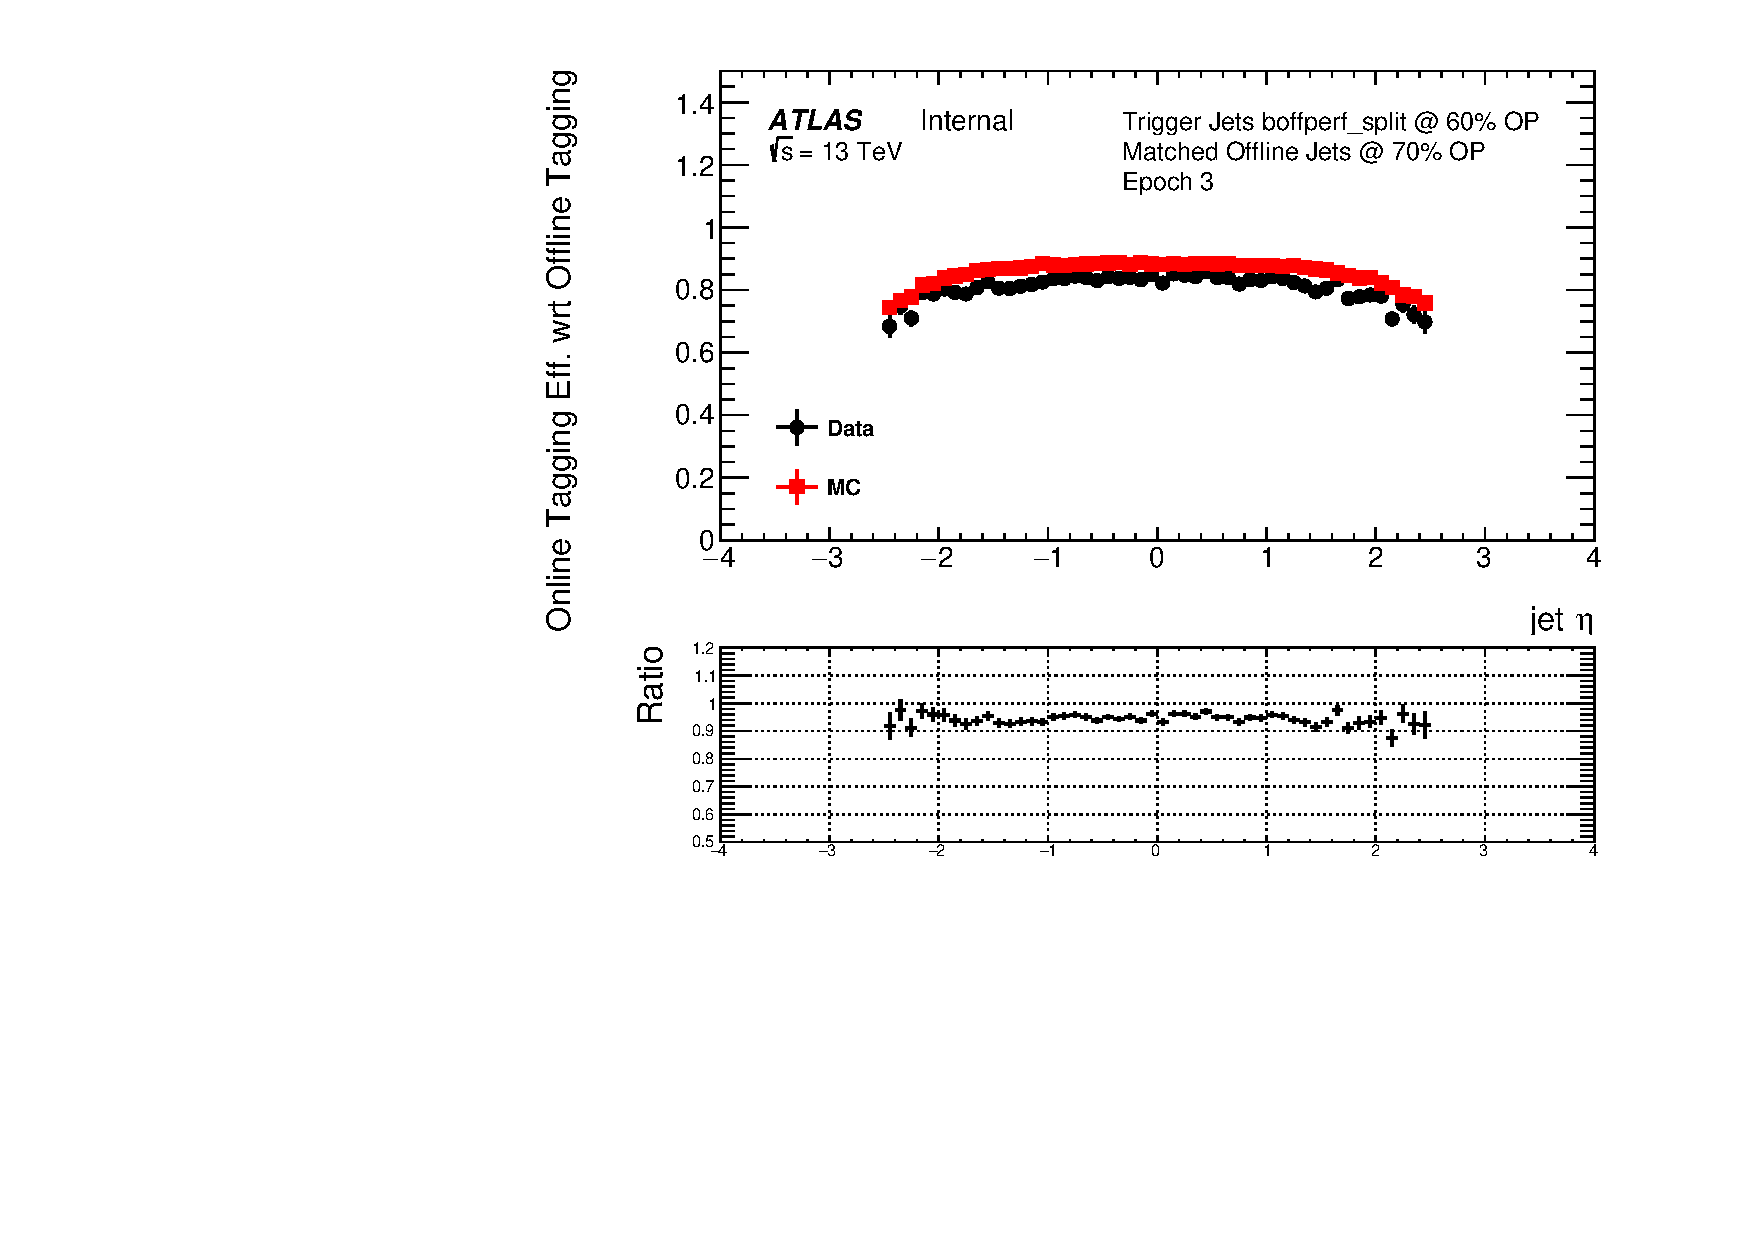
\includegraphics[width=0.47\linewidth, angle=0]{figs/Trigger/btrigger_old/Epoch3_trigReq_eff_jetEta.pdf}} \\
  \subcaptionbox{$z_{bs}^{online}$}{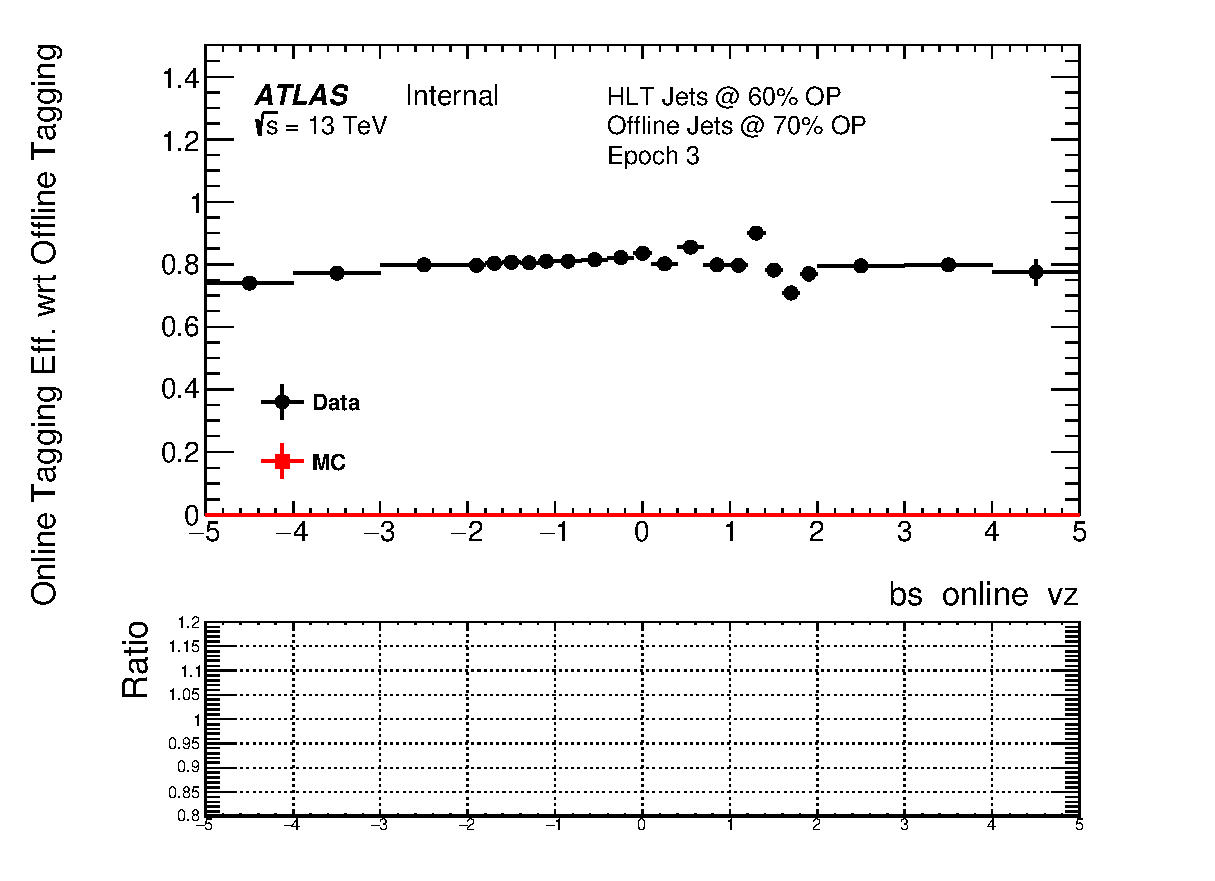
\includegraphics[width=0.47\linewidth, angle=0]{figs/Trigger/Epoch3_eff_bs_online_vz.eps}}
  \subcaptionbox{Vertex Class}{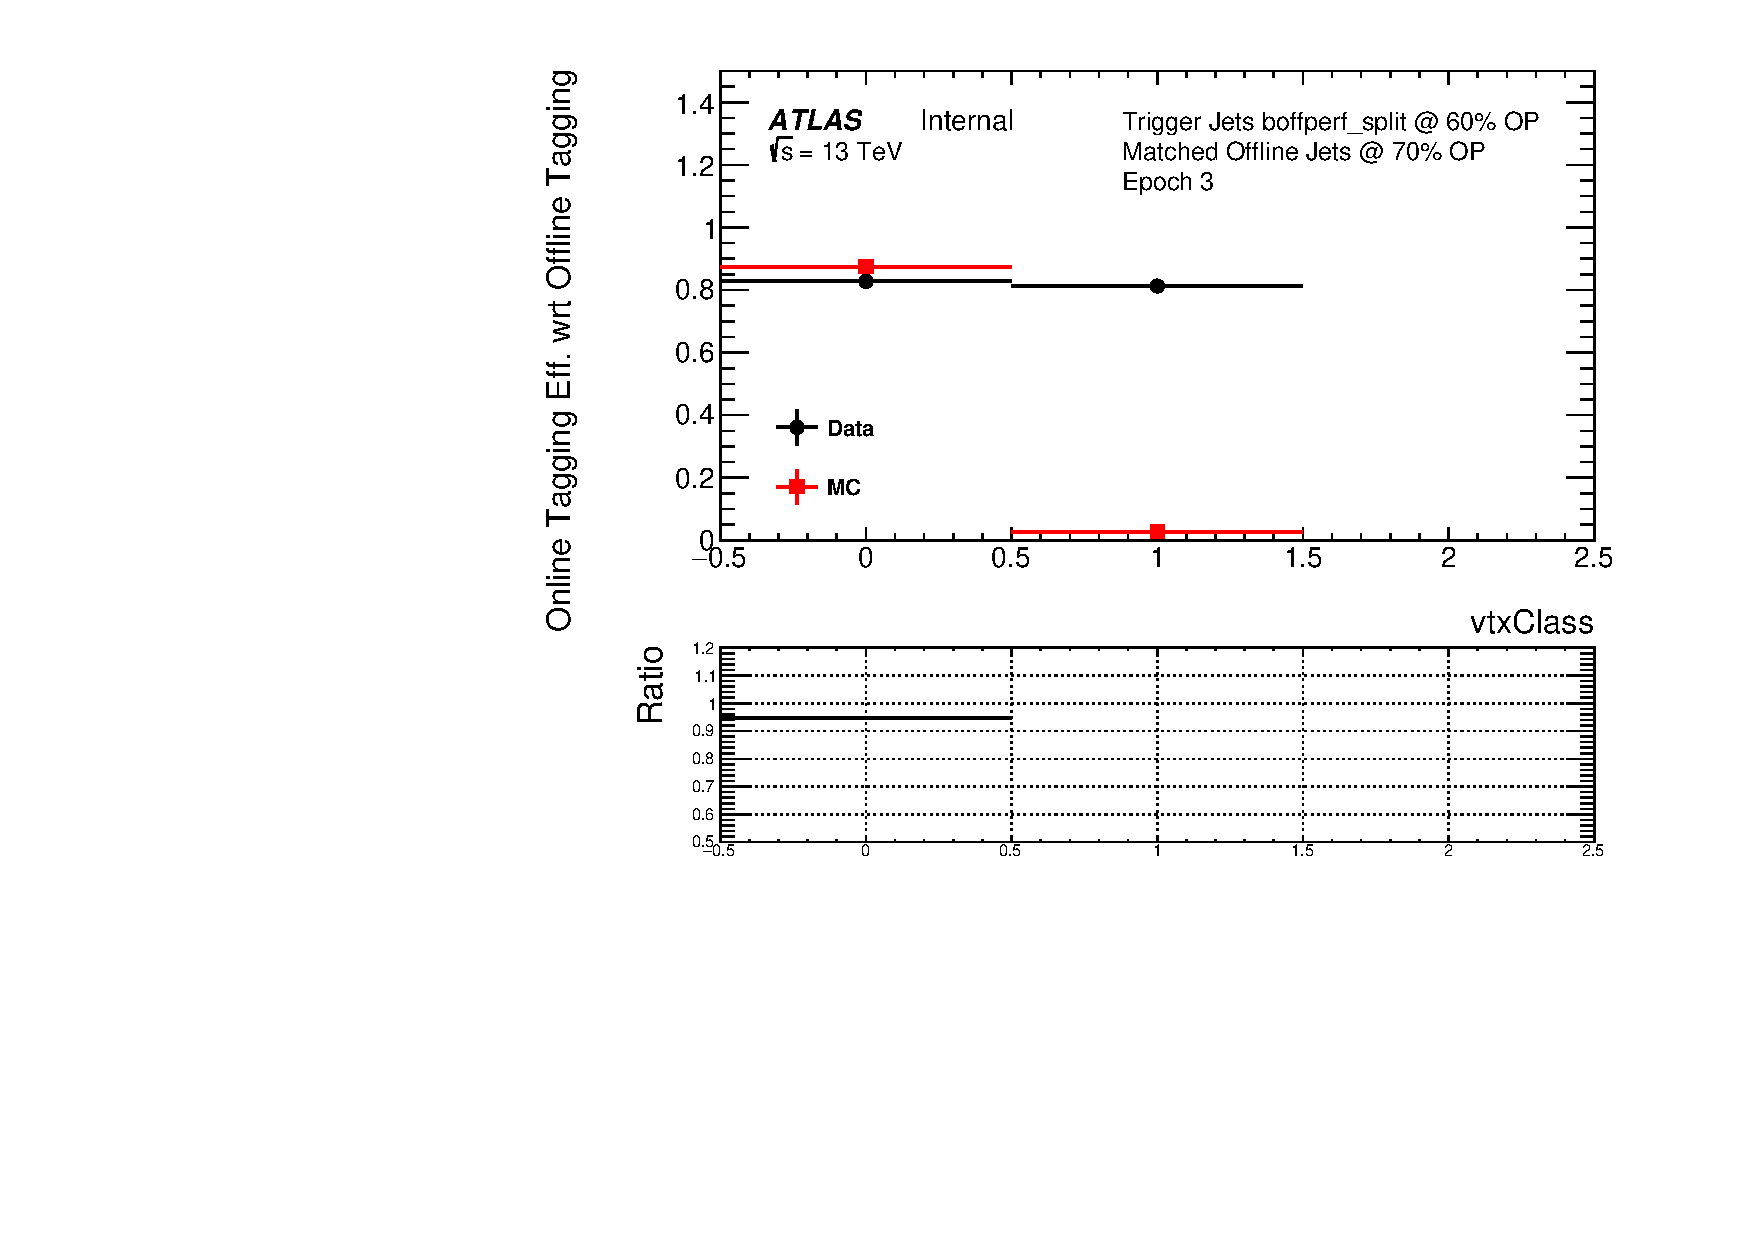
\includegraphics[width=0.47\linewidth, angle=0]{figs/Trigger/btrigger_old/Epoch3_trigReq_eff_vtxClass.pdf}}
\end{center}
\caption{The 60\% $b$-jet trigger efficiency with respect to an offline 70\% operating point tag
  for data from Epoch 3 (black) and simulation (red) against (a) jet-\pT, (b) jet-$\eta$,
  (c) online beamspot $z$-position and (d) vertex class.}
\label{fig:Epoch3_eff}
\end{figure}

\FloatBarrier

\subsection{Solution: $b$-Jet Trigger GRL}
\label{sec:trig-inv}

To summarise, in the previous section it is shown that at large values of absolute online beamspot $z$-position
the measured $\epsilon_{bTrig}$ in Epoch 1 and $\epsilon_{bPerf}$ in Epoch 2 is lower in data than in MC, due to poor \verb|xPrmVtx| PV finding performance.
In Epoch 3 there is reasonable data/simulation agreement due to the use of a backup vertex finding algorithm. 

The solution employed is to apply a $b$-jet trigger aware GRL 
that removes events with an absolute  $z_{bs}^{online}$ greater than 2mm in Epoch 1 and 2,
such that the events with low efficiency are removed.
The cost of this approach is the luminosity of our data-set is reduced, specifically the data-set falls from  32.9~\ifb to 24.3~\ifb.
However there are three key reasons why use of a $b$-jet trigger GRL was chosen over simply applying an overall efficiency.
Firstly, as there is no beamspot position distribution in simulation it is not clear that kinematics of events at high  $z_{bs}^{online}$ can be well understood and modelled;
the sculpting of the efficiency with respect to jet-$\eta$ is an example of this.
Secondly, the efficiencies are quite low at high beamspot $z$-position,
so the loss in luminosity x acceptance is relatively small
and finally the use of a GRL means a more realistic estimate of the actual luminosity used in an analysis is used. 

For the choice of which value of beamspot $z$ position to use for in the GRL,
it was required to select the widest cut where the efficiency had not significantly declined,
such that as much luminosity as possible is retained while removing most of the affected region.
This \SI{2}{\mm} cut was chosen from examining Figure~\ref{fig:Epoch1_eff}(b) and Figure~\ref{fig:Epoch2_bperf}(b)
and from studying a variety of cuts from \SI{2}{\mm} to \SI{1}{\mm}.

After the GRL is applied, $\epsilon_{bTrig}$ for Region 1 becomes approximately 90-95\% of the efficiency measured in simulation,
as shown in Figure~\ref{fig:Epoch1_bslt2mm_eff},
and $\epsilon_{bPerf}$ for Region 2 becomes approximately 95\% of the efficiency measured in simulation,
as shown in Figure~\ref{fig:Epoch2_bslt2mm_bperf}. 

\begin{figure}[!ht]
  \begin{center}
    \captionsetup[subfigure]{aboveskip=0pt,justification=centering}
    \subcaptionbox{Jet-\pT}{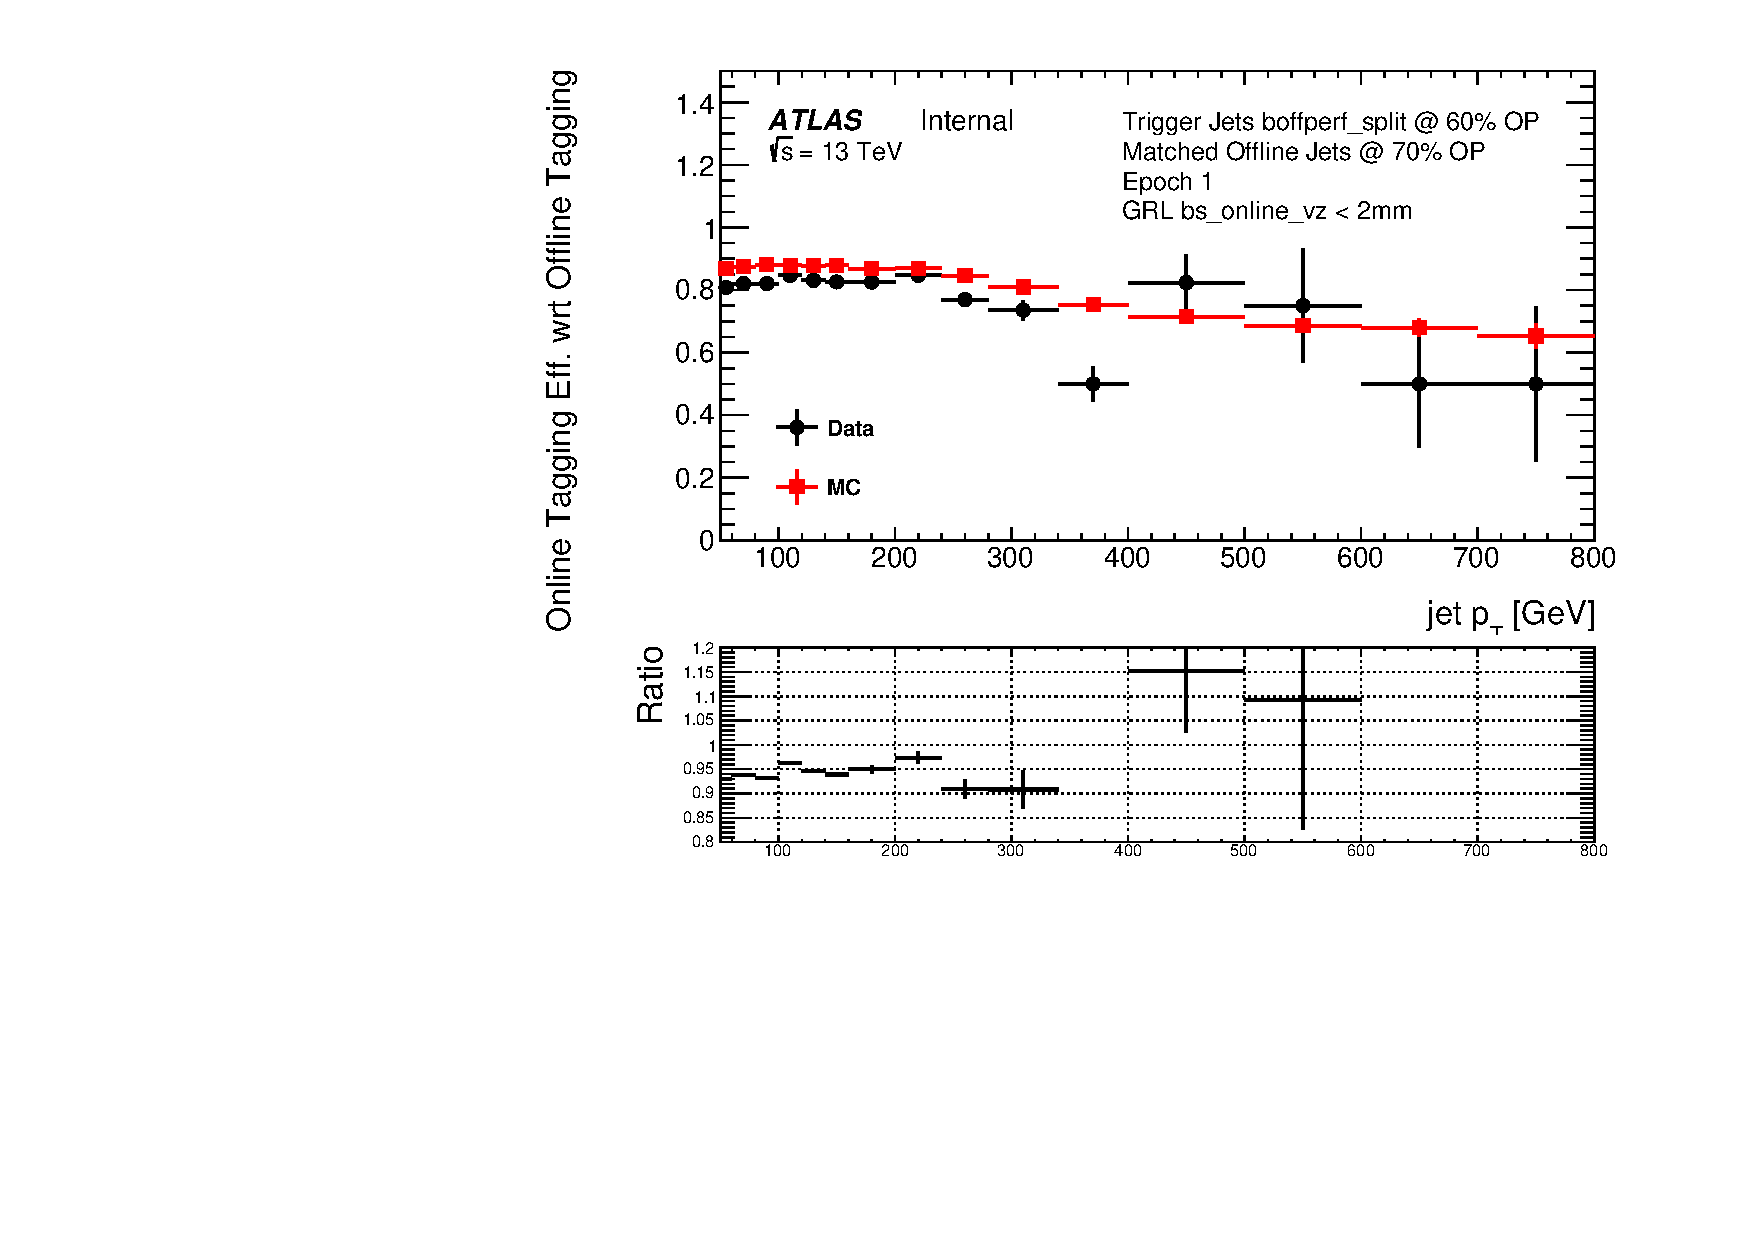
\includegraphics[width=0.47\linewidth, angle=0]{figs/Trigger/btrigger_old/Epoch1_GRL_bslt2mm_trigReq_eff_jetPt.pdf} }
    \subcaptionbox{Jet-$\eta$}{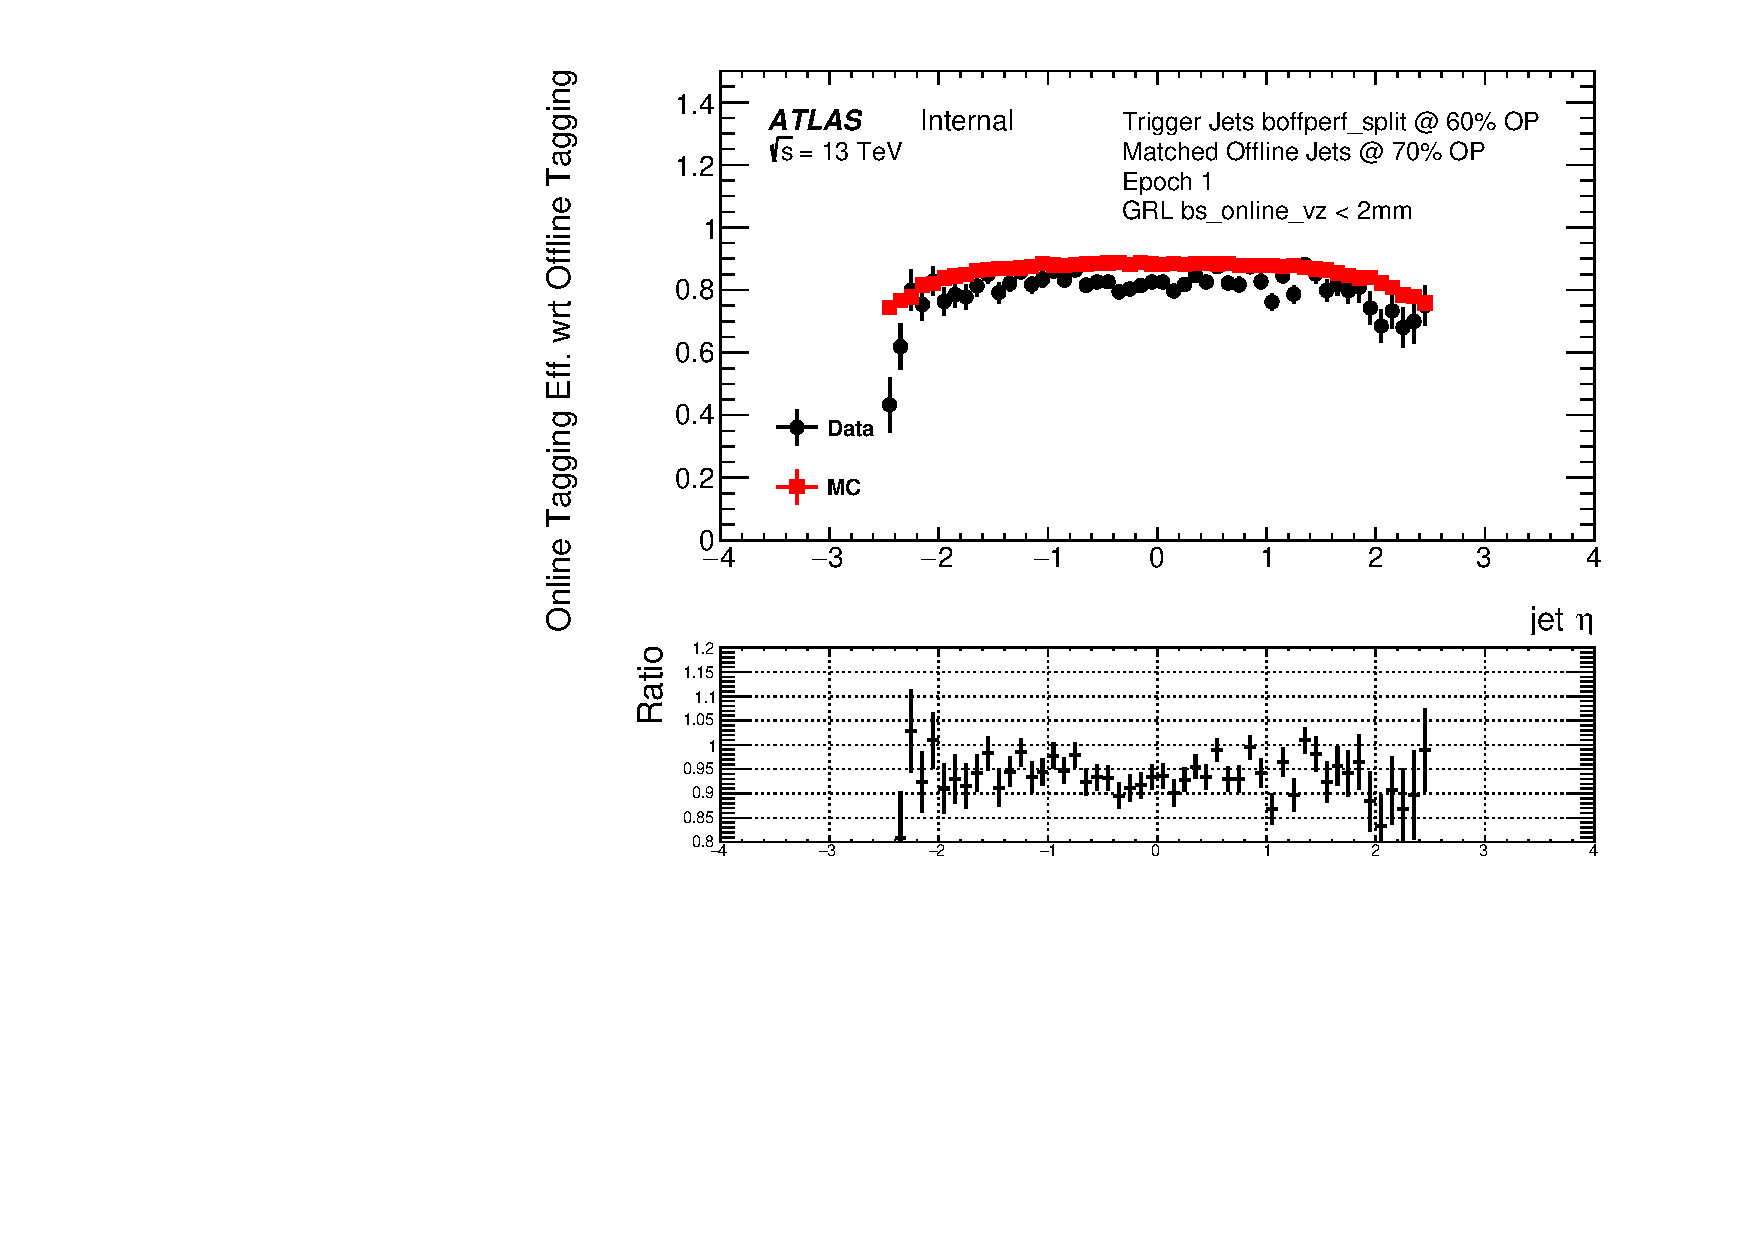
\includegraphics[width=0.47\linewidth, angle=0]{figs/Trigger/btrigger_old/Epoch1_GRL_bslt2mm_trigReq_eff_jetEta.pdf}}
  \end{center}
  \caption{The 60\% $b$-jet trigger efficiency with respect to an offline 70\% operating point tag
    for data from Region 1 (black) and simulation (red) against jet-\pT~(a) and jet-$\eta$ (b).
    The $b$-jet trigger aware GRL has been applied.}
  \label{fig:Epoch1_bslt2mm_eff}
  \begin{center}
    \captionsetup[subfigure]{aboveskip=0pt,justification=centering}
    \subcaptionbox{Leading Jet-\pT}{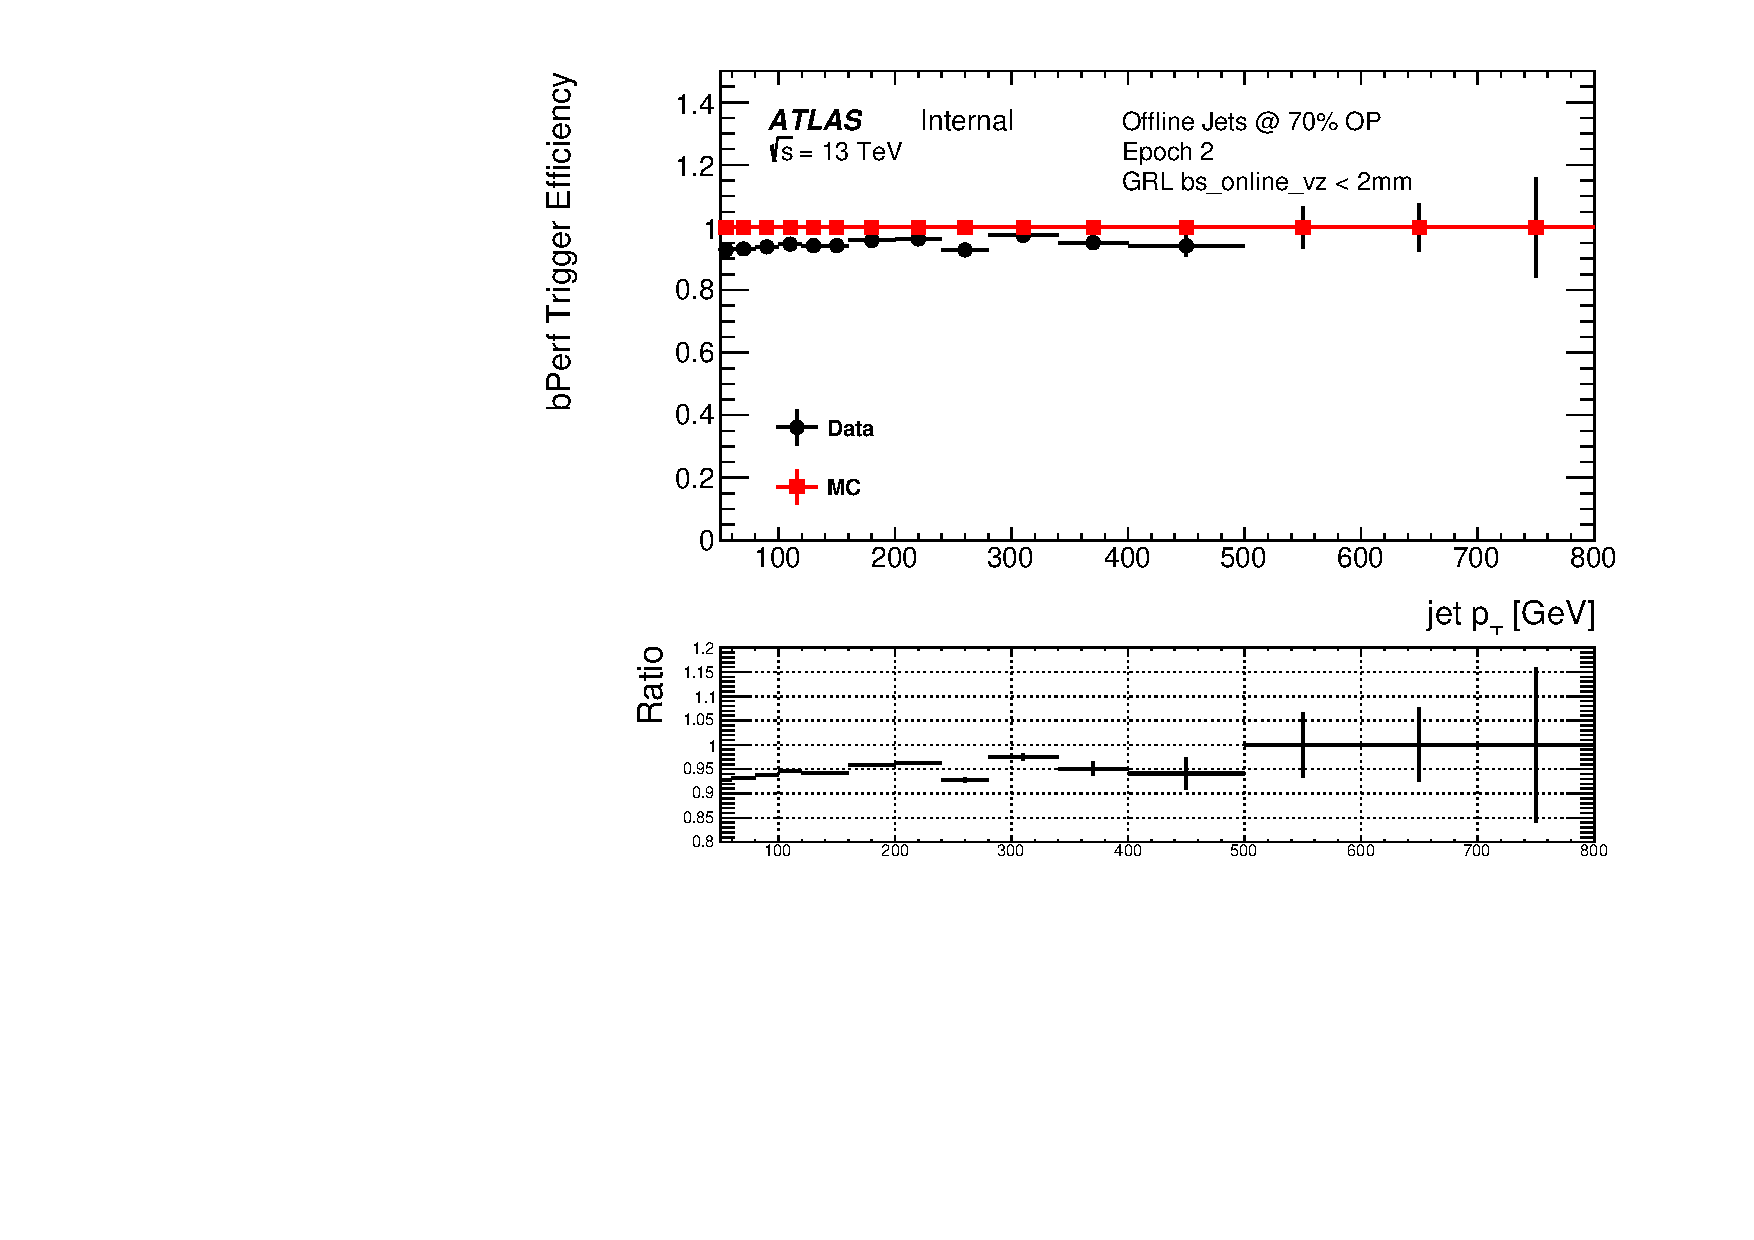
\includegraphics[width=0.47\linewidth, angle=0]{figs/Trigger/btrigger_old/Epoch2_GRL_bslt2mm_trigReq_bPerfEff_jetPt.pdf} }
    \subcaptionbox{Leading Jet-$\eta$}{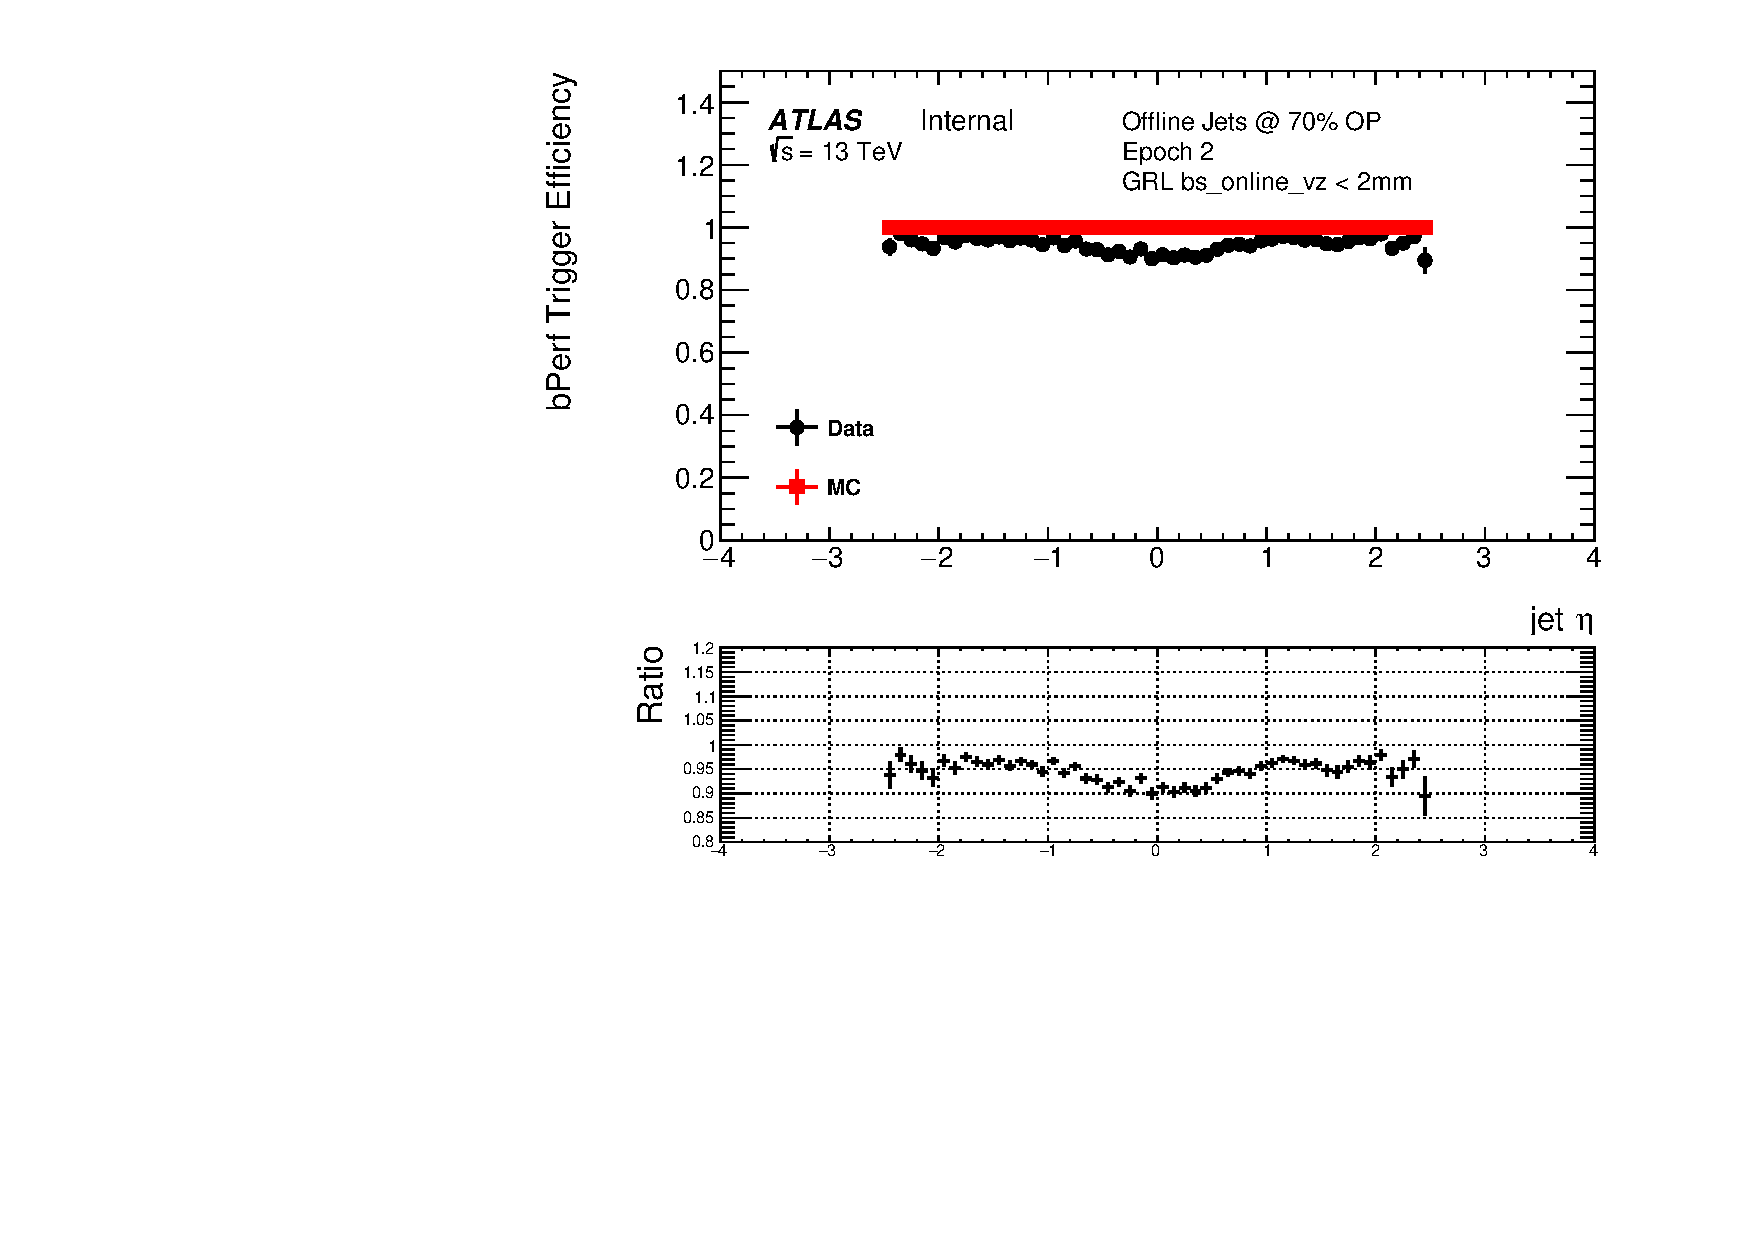
\includegraphics[width=0.47\linewidth, angle=0]{figs/Trigger/btrigger_old/Epoch2_GRL_bslt2mm_trigReq_bPerfEff_jetEta.pdf}}
  \end{center}
  \caption{$b$-perf efficiency, $\epsilon_{bPerf}$, for data from Region 2 (black) and simulation (red) against leading (a) jet-\pT~and (b) jet-$\eta$.
    The $b$-jet trigger aware GRL has been applied.}
  \label{fig:Epoch2_bslt2mm_bperf}
\end{figure}

\newpage

Figures~\ref{fig:Full_bslt2mm_eff} and ~\ref{fig:Full_bslt2mm_bperf}  shows measured
$\epsilon_{bPerf}$ and $\epsilon_{bTrig}$
for the full 2016 data-set, combining Regions 1, 2 and 3,
with the $b$-jet trigger aware GRL applied.
This represents the raw observed data/simulation efficiencies when the full event selection has been applied.

\begin{figure}[!ht]
  \begin{center}
    \captionsetup[subfigure]{aboveskip=0pt,justification=centering}
    \subcaptionbox{Jet-\pT}{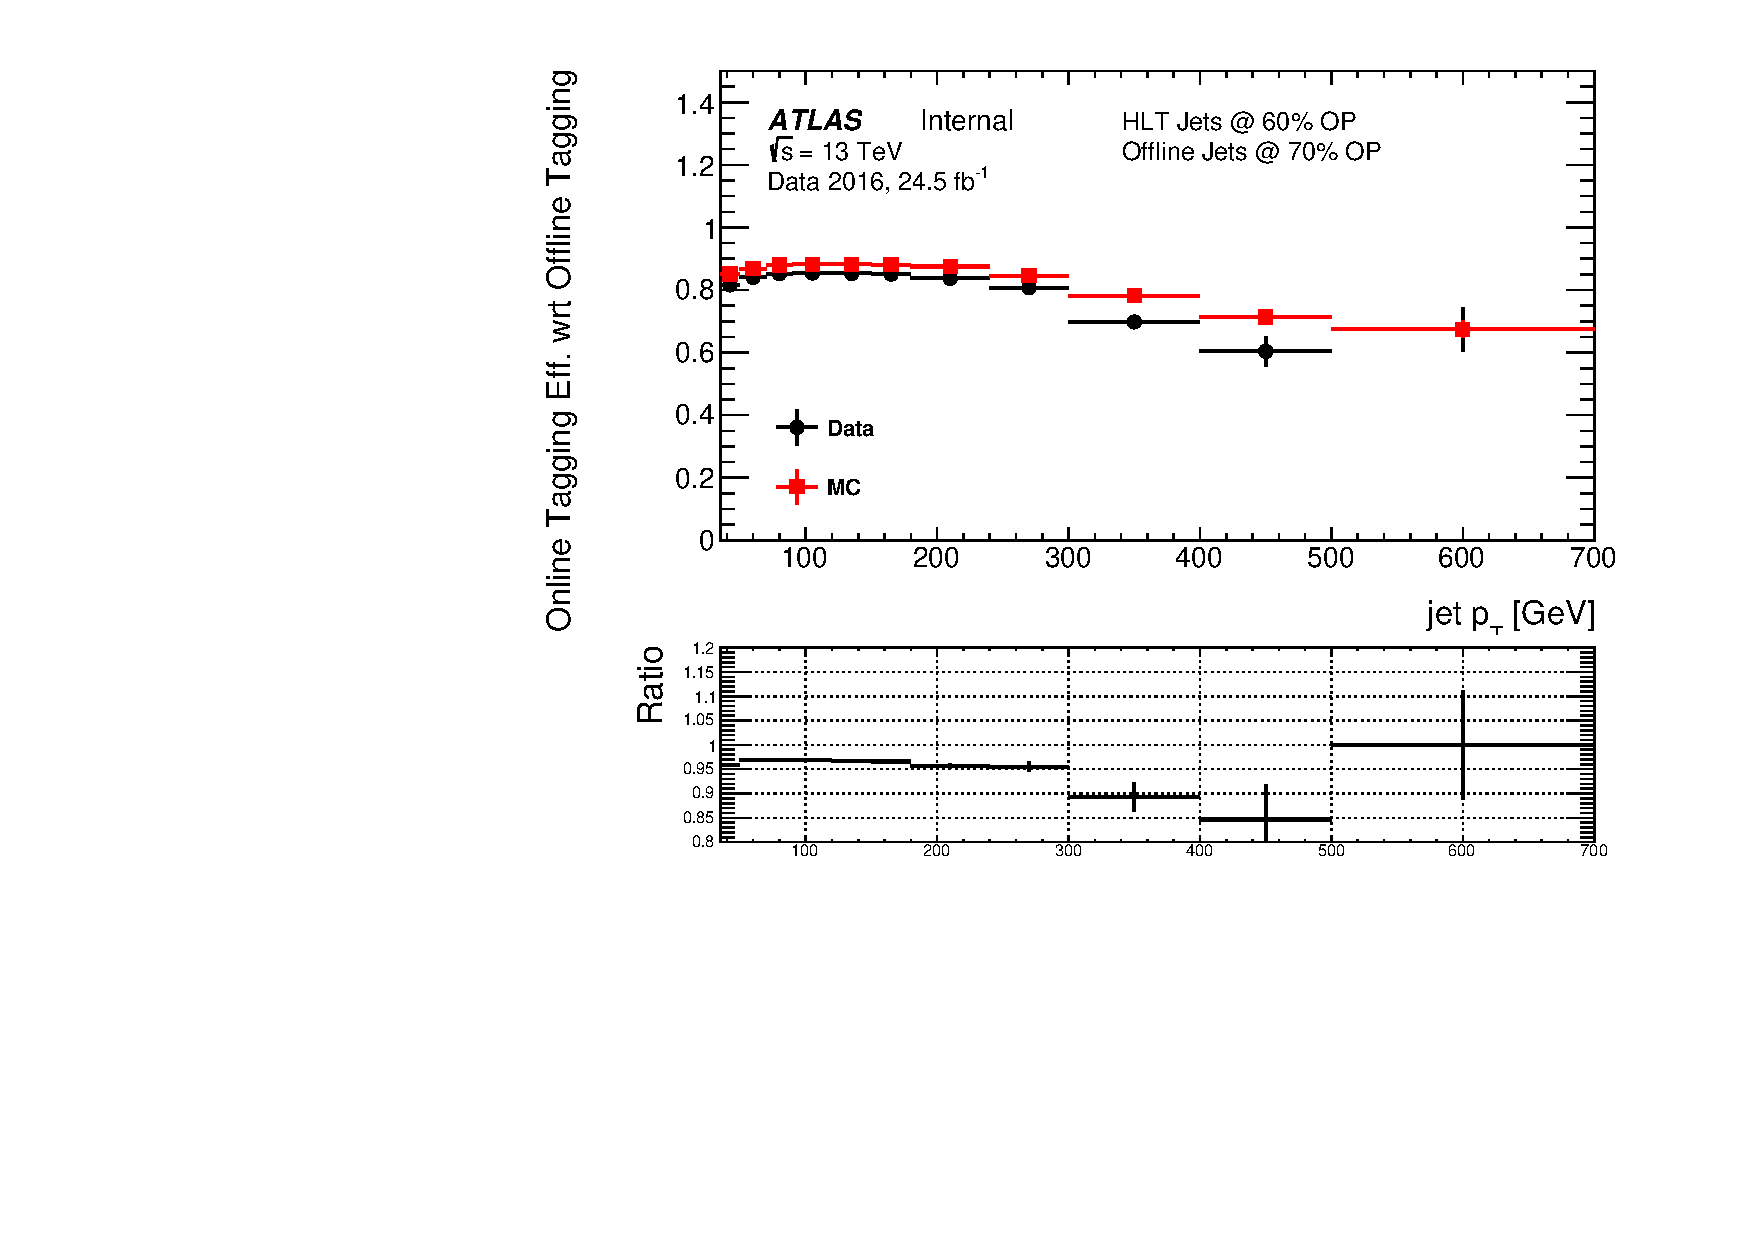
\includegraphics[width=0.47\linewidth, angle=0]{figs/Trigger/btrigger_old/Full_GRL_bslt2mm_trigReq_eff_jetPt.pdf}}
    \subcaptionbox{Jet-$\eta$}{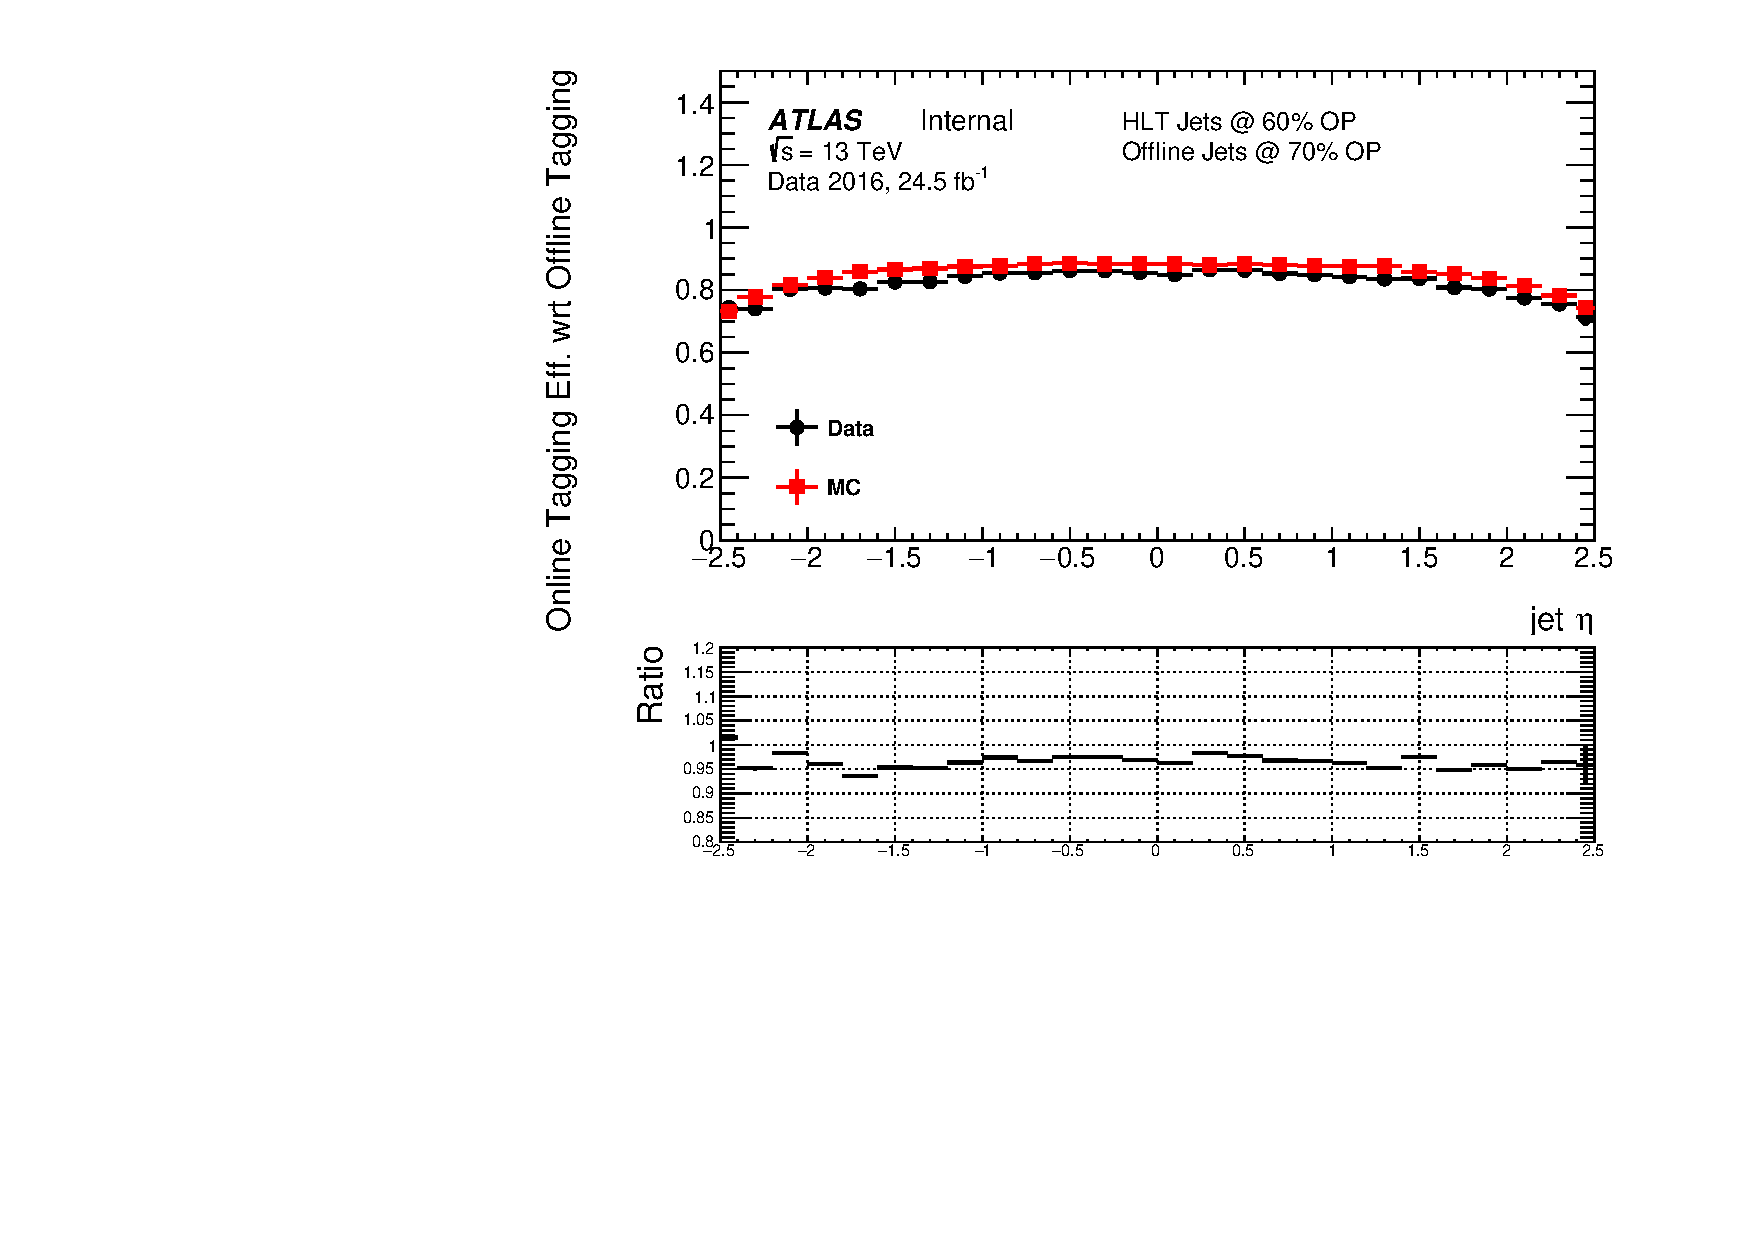
\includegraphics[width=0.47\linewidth, angle=0]{figs/Trigger/btrigger_old/Full_GRL_bslt2mm_trigReq_eff_jetEta.pdf}}\\
    \subcaptionbox{$z_{bs}^{online}$}{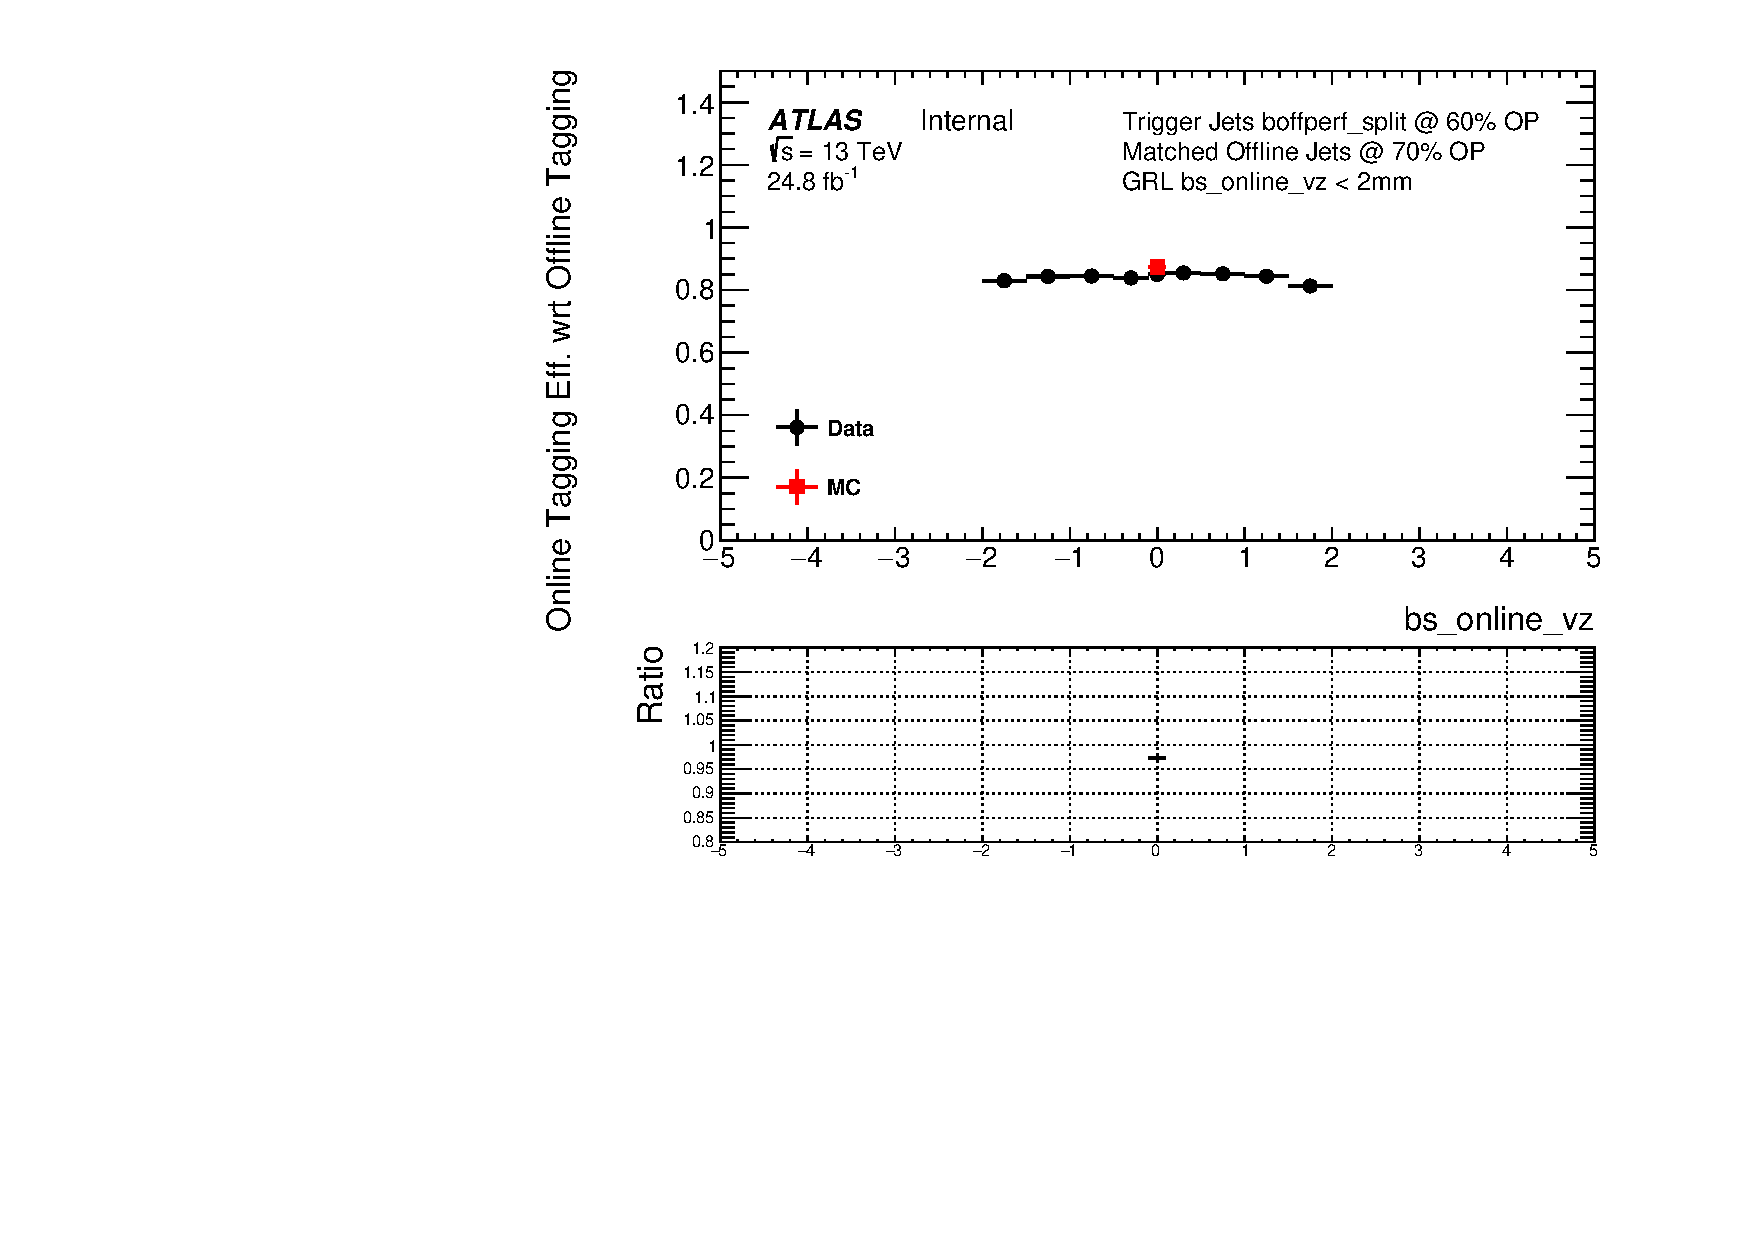
\includegraphics[width=0.47\linewidth, angle=0]{figs/Trigger/btrigger_old/Full_GRL_bslt2mm_trigReq_eff_bs_online_vz.pdf}}
    \subcaptionbox{Vertex Class}{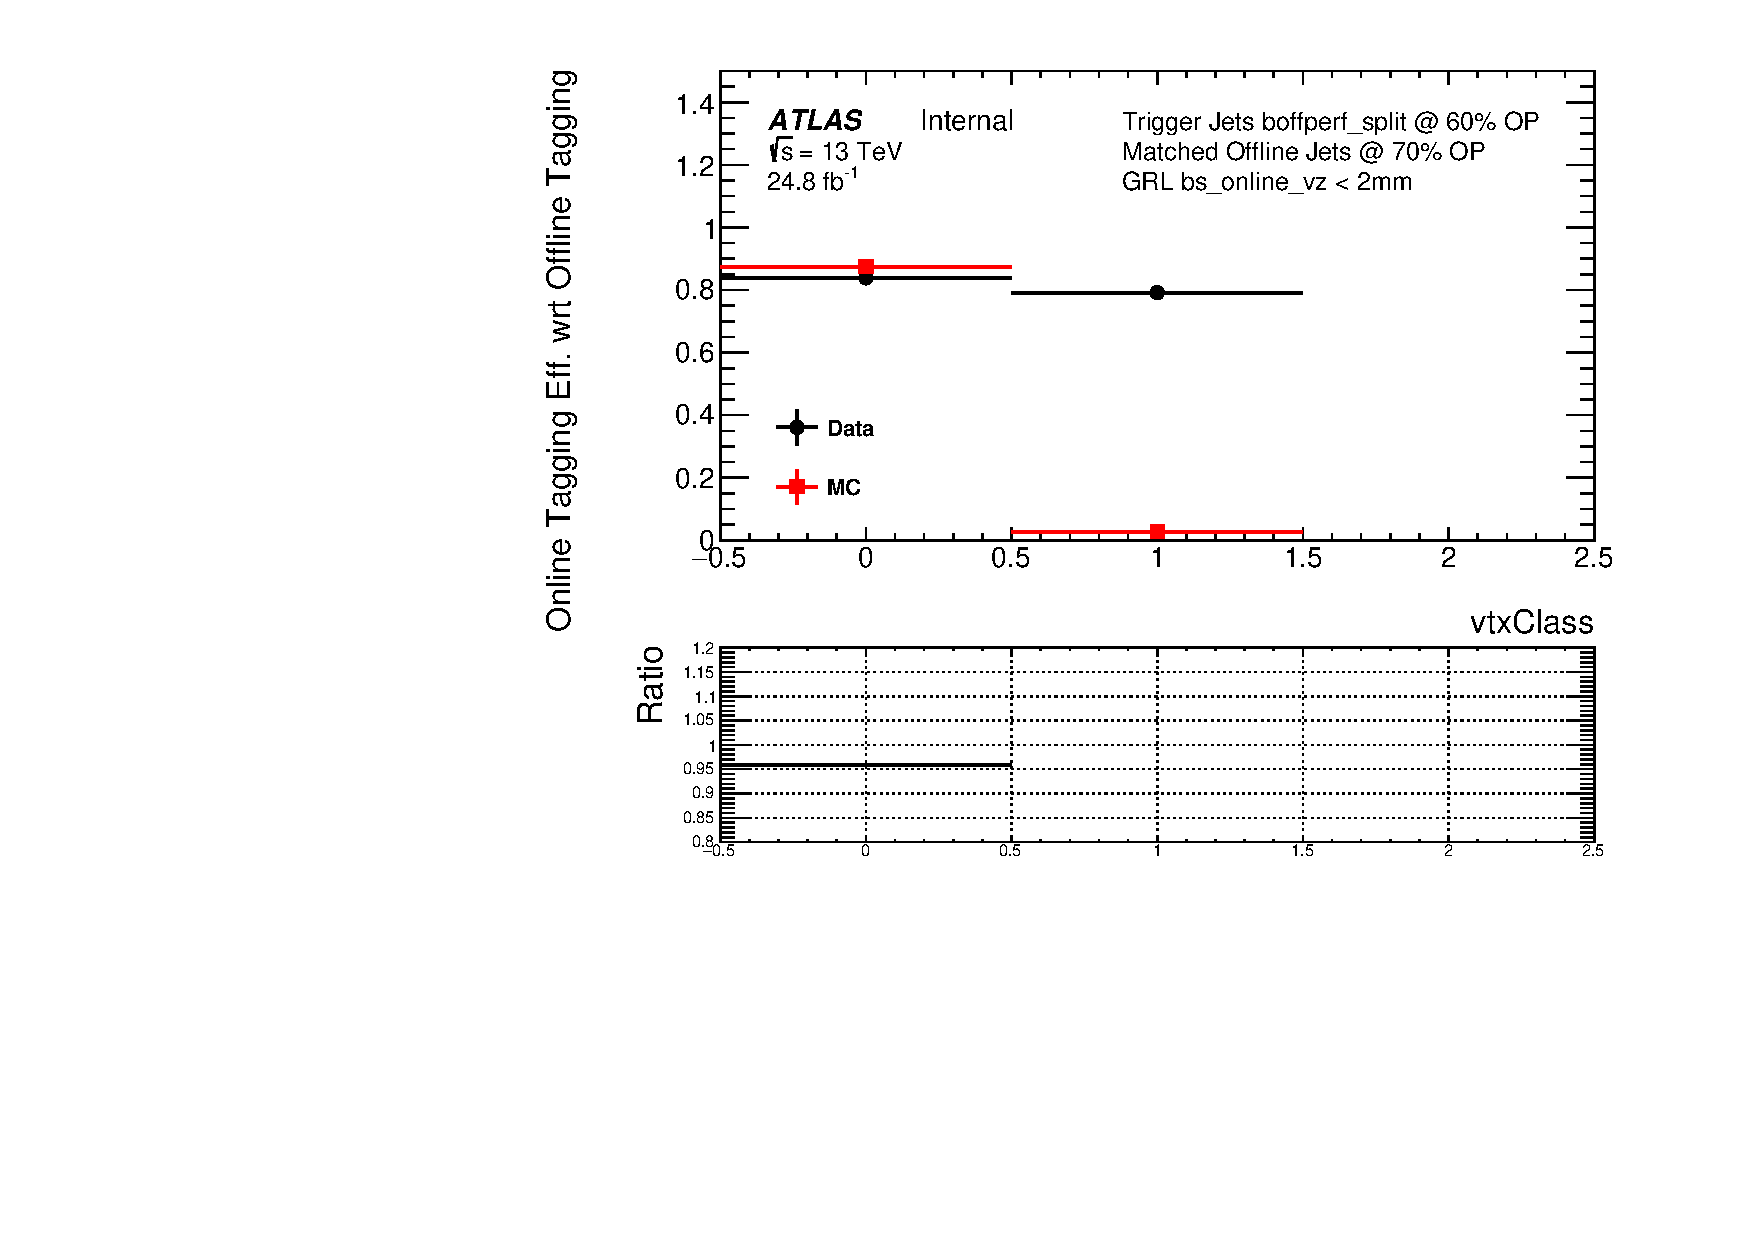
\includegraphics[width=0.47\linewidth, angle=0]{figs/Trigger/btrigger_old/Full_GRL_bslt2mm_trigReq_eff_vtxClass.pdf}}
  \end{center}
  \caption{The 60\% $b$-jet trigger efficiency with respect to an offline 70\% operating point tag
    for the full 2016 data-set (black) and simulation (red) against jet-\pT~(a), jet-$\eta$ (b), online beamspot $z$-position (c) and vertex class (d).}
  \label{fig:Full_bslt2mm_eff}
  \begin{center}
    \captionsetup[subfigure]{aboveskip=0pt,justification=centering}
    \subcaptionbox{Leading Jet-\pT}{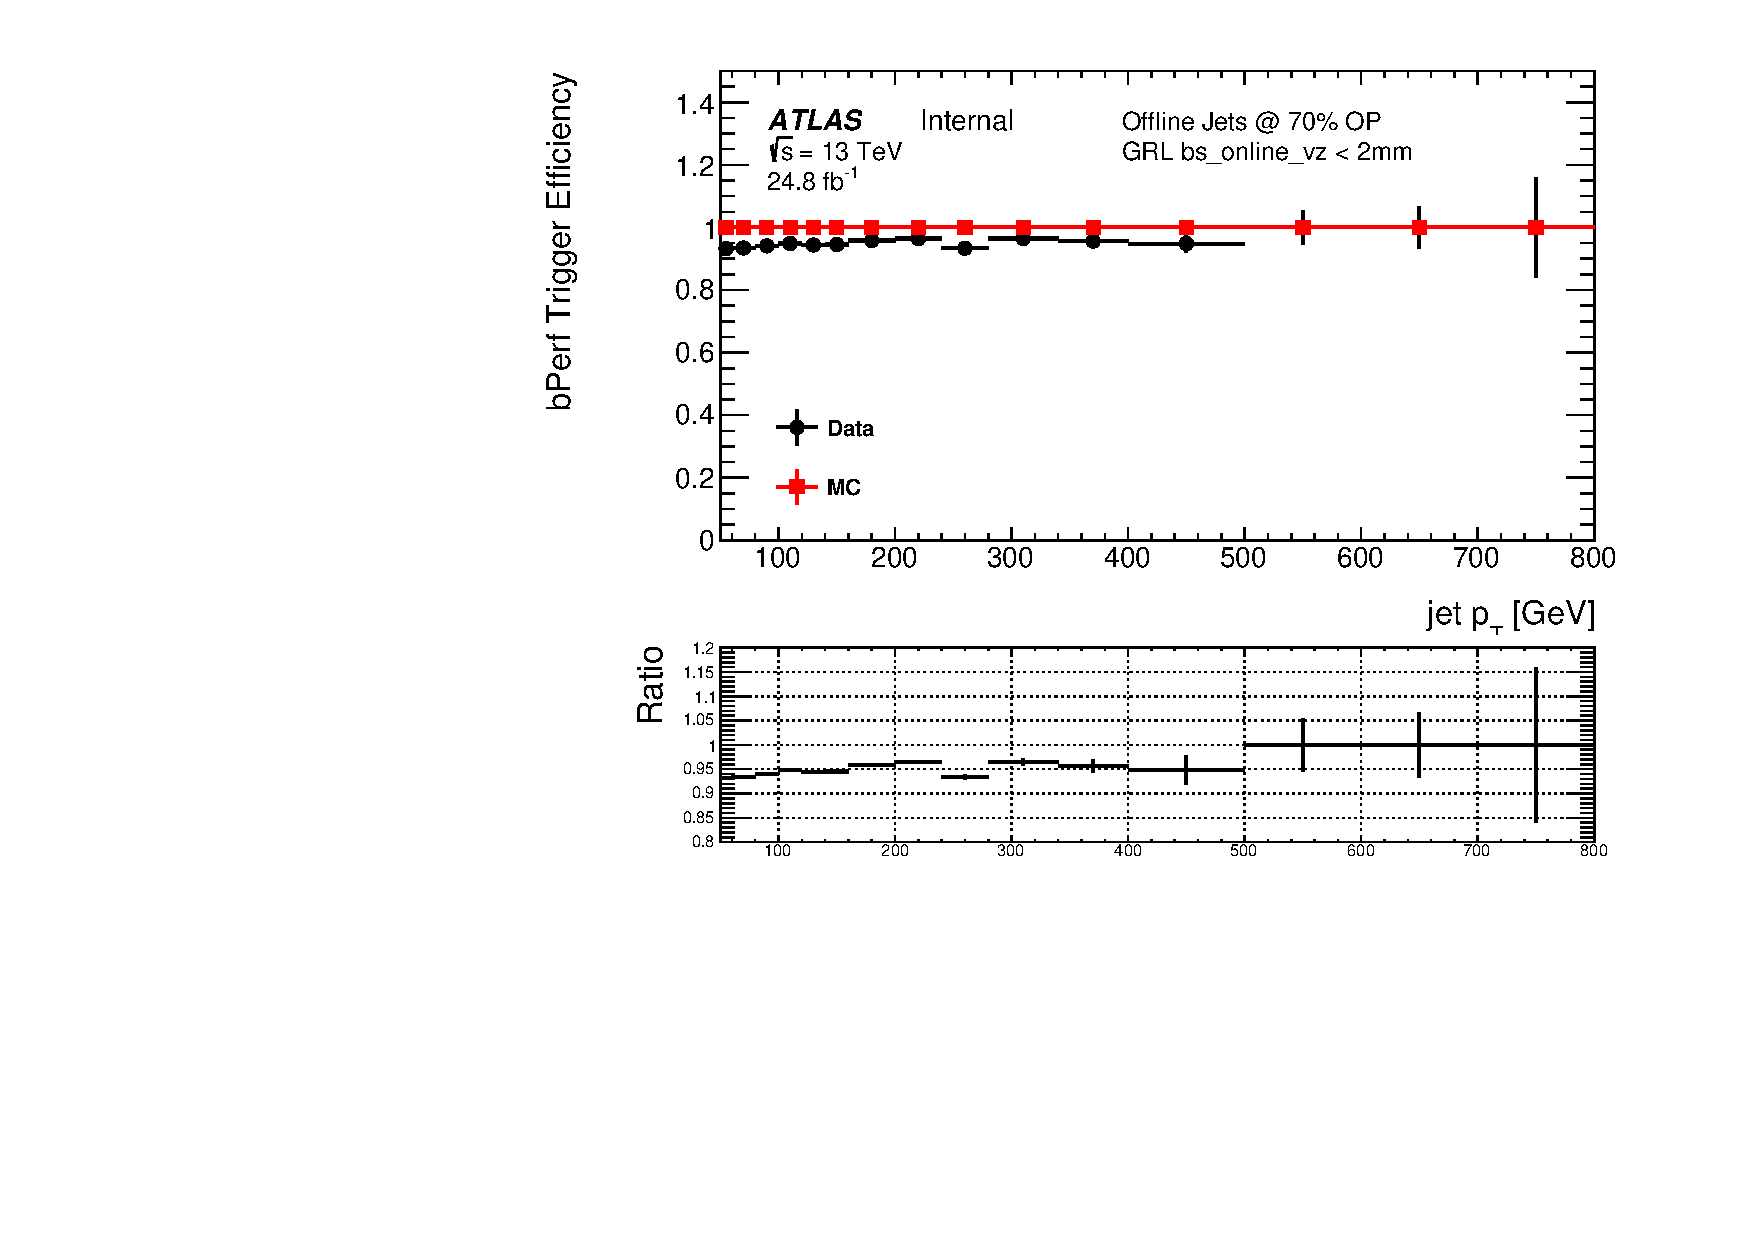
\includegraphics[width=0.47\linewidth, angle=0]{figs/Trigger/btrigger_old/Full_GRL_bslt2mm_trigReq_bPerfEff_jetPt.pdf}}
    \subcaptionbox{Leading Jet-$\eta$}{\includegraphics[width=0.47\linewidth, angle=0]{figs/Trigger/btrigger_old/Full_GRL_bslt2mm_trigReq_bPerfEff_jetEta.pdf}}
  \end{center}
  \caption{$b$-perf efficiency, $\epsilon_{bPerf}$, for the full 2016 data-set (black) and simulation (red) against (a) leading jet-\pT~and (b) jet-$\eta$.
    The $b$-jet trigger aware GRL has been applied.}
  \label{fig:Full_bslt2mm_bperf}
\end{figure}
  

\FloatBarrier
\newpage

\subsection{Efficiency Measurement and Systematic Derivation}
In the previous two sections it has been shown that when applying a $b$-jet aware GRL,
the $b$-jet trigger performance is understood and the data/simulation agreement is within 5\%.
In this section the measurement of data efficiency, data/simulation scale factors (SFs)
and associated systematics to account for the 5\% are described.

As discussed above, there are two factors considered in this section.
Firstly there is the $\epsilon_{bTrig}$ measurement
that accounts for differences in online and offline $b$-tagging given that a valid primary vertex has been found.
Sections~\ref{sec:trig-purity}~to~\ref{sec:trig-highPtExtrap} describes the derivation of a set of systematics and corrections to the raw measurement
and Section~\ref{sec:trig-jetLevelEff} presents the final measurement, which is applied as a jet-level efficiency in the final analysis.
Secondly, in Section~\ref{sec:trig-eventLevelEff}, is a description the measurement of the $\epsilon_{bPerf}$ that accounts
for the efficiency of finding a valid primary vertex and the relevant systematics, which is applied as an event level efficiency.

In this section describing the final measurement, the full 2016 data set is used,
the simulated ${t\bar{t}}$ sample includes single-top processes
and the full event selection from Section~\ref{sec:trig-evtSel} is applied.

% This section got cut and moved to jetLevelEff
%\subsubsection{$\eta$ Dependence on Efficiency}
%\label{sec:trig-etaDep}
%\begin{figure}[!ht]
%  \begin{center}
%    \includegraphics[width=0.47\linewidth, angle=0]{figs/Trigger/btrigger_old/Full_GRL_bslt2mm_trigReq_eff_jetPt.pdf}
%    \includegraphics[width=0.47\linewidth, angle=0]{figs/Trigger/btrigger_old/Full_GRL_bslt2mm_trigReq_eff_jetEta.pdf}
%  \end{center}
%  \caption{The 60\% $b$-jet trigger efficiency with respect to an offline 70\% operating point tag
%    for data from Periods A-L (black) and simulation (red) against jet-\pT~(a), jet-$\eta$ (b).}
%  \label{fig:Full_bslt2mm_eff_eta}
%\end{figure}

\subsubsection{Purity Error}
\label{sec:trig-purity}

It is known that despite the strict event selection there will inevitably be non b-jet contamination in our sample.
To estimate the b-jet purity simulation is used, where the true flavour of the jet is available.
Jets as categorised as true $b$-jets, meaning that a $B$-hadron was found within a cone of R = 0.4, or true non-b-jets if not.
Then distributions for inclusive jets to the truth matched b-jets in the simulation sample are compared.
Figure~\ref{fig:Purity} shows the b-jet purity for jet-\pT~and jet-$\eta$;
showing that the b-jet purity is $>$ 95\% up to jet-\pT$\sim$300~\GeV~and $>$ 90\% for higher values of jet-\pT.

To estimate the effect of these impurities on the efficiency measurement simulation is again used.
Firstly, the efficiency in our nominal inclusive simulation is compared
to the efficiencies if only true-b-jets or true non-b-jets are selected,
this is shown if Figure~\ref{fig:Eff_Purity}(a).
The ratio is applied as a correction to the final efficiency measurement.
Then any mismodelling of the  $b$-jet fraction in simulation is also considered,
to account for this the efficiency for the simulated inclusive sample is compared to the efficiency when the non b-jet content has been doubled, as shown in Figure~\ref{fig:Eff_Purity}(b).
The maximum difference from the efficiency measured in the inclusive simulated sample and the cases
where there is only true b-jets and where the non b-jet content has been doubled,
shown in the two ratio plots in Figure~\ref{fig:Eff_Purity}, is taken as a symmetric systematic.

\begin{figure}[!ht]
  \begin{center}
    \captionsetup[subfigure]{aboveskip=0pt,justification=centering}
    \subcaptionbox{Jet-\pT}{\includegraphics[width=0.47\linewidth, angle=0]{figs/Trigger/btrigger_old/PurityMC_jetPt.pdf}}
    \subcaptionbox{Jet-$\eta$}{\includegraphics[width=0.47\linewidth, angle=0]{figs/Trigger/btrigger_old/PurityMC_jetEta.pdf}}
  \end{center}
  \caption{A comparison of offline jets tagged at the 70\% operating point
    for inclusive jets (red) and truth-matched b-jets (blue)
    against jet-\pT~(a) and jet-$\eta$ (b) in a simulated $t\bar{t}$ sample.}
  \label{fig:Purity}
  \begin{center}
    \captionsetup[subfigure]{aboveskip=0pt,justification=centering}
    \subcaptionbox{}{\includegraphics[width=0.47\linewidth, angle=0]{figs/Trigger/btrigger_old/EffMC_jetPt_trueB.pdf}}
    \subcaptionbox{}{\includegraphics[width=0.47\linewidth, angle=0]{figs/Trigger/btrigger_old/EffMC_jetPt_2nonB.pdf}}
  \end{center}
  \caption{The 60\% $b$-jet trigger efficiency with respect to an offline 70\% operating point tag
    for inclusive jets (black) compared to truth matched b-jets and non b-jets (a) and the case where non b-jet content has been doubled (b) for a simulated $t\bar{t}$ sample.
    The lower panel in both plots show the ratio to the inclusive efficiency.
  }
  \label{fig:Eff_Purity}
\end{figure}

\subsubsection{Non-b-jet trigger efficiency error}
\label{sec:trig-lightTrigEff}

As one would expect and as shown in left plot of Figure~\ref{fig:Eff_Purity}, non b-jets (shown in blue) have a different b-jet trigger efficiency to that of b-jets.
However the exact efficiency is not known well and could be mismodelled in simulation.
To account for this uncertainty the nominal efficiency in simulation is compared
to the cases where the non-b-jet efficiency has been halved and doubled in simulation, as shown in Figure~\ref{fig:Eff_LTrigEff}.
When doubling the non-b-jet trigger efficiency this is limited at the upper end to being no greater than the true b-jet trigger efficiency.
The maximum bin-by-bin difference between the nominal and the two cases, as shown in the two ratio plots, is taken as a systematic.

\begin{figure}[!ht]
  \begin{center}
    \captionsetup[subfigure]{aboveskip=0pt,justification=centering}
    \subcaptionbox{}{\includegraphics[width=0.47\linewidth, angle=0]{figs/Trigger/btrigger_old/effMC_jetPt_lowLTrigEff.pdf}}
    \subcaptionbox{}{\includegraphics[width=0.47\linewidth, angle=0]{figs/Trigger/btrigger_old/effMC_jetPt_upLTrigEff.pdf}}
  \end{center}
  \caption{The 60\% $b$-jet trigger efficiency with respect to an offline 70\% operating point tag
    for nominal inclusive case (black) compared to varied inclusive case (red) and just non b-jets (blue)
    in the case where non b-jet efficiency has been halved (a) and doubled (b) for a simulated $t\bar{t}$ sample.
    The lower panel in both plots show the ratio of the varied inclusive efficiency to the nominal inclusive efficiency.
  }
  \label{fig:Eff_LTrigEff}
\end{figure}

\FloatBarrier

\subsubsection{High-\pT~extrapolation}
\label{sec:trig-highPtExtrap}

Measuring $b$-jet trigger efficiency for high-\pT~jets is limited by the statistics in the simulated $t\bar{t}$ sample,
so the shape from simulation will be used to extrapolate the efficiency for jet-\pT $>$ 240 GeV.
The point from which to extrapolate from was chosen as this is when data statistic error starts to become large. 

The procedure is made of two sequential fits (normalisation and correction) to the data/simulation ratio,
which are used to create a ``corrected simulation'' $\epsilon_{bTrig}$ distribution.
For jet-$pT$ $>$ 240 GeV, the corrected $\epsilon_{bTrig}$ is used in place of data when measuring the data $\epsilon_{bTrig}$ efficiency
and when calculating data/MC scale factors.
A final quadratic fit is used to assign a systematic. 

\noindent
In more detail:
\begin{itemize}
  \setlength\itemsep{1em}
\item \textbf{Flat Normalisation Fit}: \\
  The measured $\epsilon_{bTrig}$, in both data and simulation are compared,
  and a horizontal fit is performed to the ratio of the two.
  The fit range is set at $\pT > 50\GeV$ to discount the first bin, which has a larger purity uncertainty.
  This is then used to normalise the simulated efficiency distribution to match data.
  This fit is shown in the lower plot  of panel (a) in Figure~\ref{fig:bTrig_mcExtrap}.
  The error on the one parameter of this fit is taken as a systematic error.
  
\item \textbf{Linear Correction Fit}:  \\
  The measured $\epsilon_{bTrig}$, in both data and the normalised simulation are compared,
  and a linear fit is performed to the ratio of the two from jet-\pT $>$ 240 GeV.
  This is then used to correct the simulated efficiency distribution to match data.
  This fit is shown in the lower plot of panel (b) in Figure~\ref{fig:bTrig_mcExtrap}.
  The simulated $\epsilon_{bTrig}$, after both the normalisation and linear correction is referred to as the corrected simulation.
  To assign a systematic on the fit parameters, the slope of this fit is varied up and down within errors,
  whilst the point at which the fit crosses 1 is kept constant.
  The maximum difference between the nominal fit and the varied fits is taken as the error on the linear correction fit.
  Panel (c) of Figure~\ref{fig:bTrig_mcExtrap} shows the data compared to the corrected simulation.
  The lower panel shows the ratio of the two, and the blue lines represent the errors on the linear correction fit.
  
\item \textbf{Quadratic Systematic Fit}: \\
  Finally to assess an error on the choice of a linear fit as the functional form above,
  a fit is performed to the data and corrected simulation ratio using a quadratic function.
  This ratio and the fit is shown in panel (d) of Figure~\ref{fig:bTrig_mcExtrap}.
  The difference of the fit from 1 is considered as the functional form error when assigning as systematic.
  
\end{itemize}

The systematic error on the extrapolation is defined as the error from normalisation fit
added to the bin-by-bin maximum of the error from the linear correction fit and the error from the quadratic systematic fit.
The errors on the high-\pT~extrapolation procedure are summarised in Table~\ref{tab:bTrig_extrapSyst}
  
\begin{figure}[!ht]
\begin{center}
\captionsetup[subfigure]{aboveskip=0pt,justification=centering}
  \subcaptionbox{Data/MC with normalisation fit} {\includegraphics[width=0.47\linewidth, angle=0]{figs/Trigger/btrigger_old/Full_GRL_bslt2mm_trigReq_effFit_jetPt.pdf} }
  \subcaptionbox{Data/normalised MC with linear correction fit} {\includegraphics[width=0.47\linewidth, angle=0]{figs/Trigger/btrigger_old/Full_GRL_bslt2mm_trigReq_effNormFit_jetPt.pdf}} \\
  \subcaptionbox{Data/corrected MC with linear correction fit errors} {\includegraphics[width=0.47\linewidth, angle=0]{figs/Trigger/btrigger_old/Full_GRL_bslt2mm_trigReq_effCorrShapeErr_jetPt.pdf}}
  \subcaptionbox{Data/corrected MC with quadratic fit } {\includegraphics[width=0.47\linewidth, angle=0]{figs/Trigger/btrigger_old/Full_GRL_bslt2mm_trigReq_effCorrFitQuad_jetPt.pdf}}
\end{center}
\caption{A figure to demonstrate the high-\pT~extrapolation procedure for the 60\% $b$-jet trigger efficiency with respect to an offline 70\% operating point tag.
  Data (black) is compared against simulation (red) after various corrections have been applied  as a function of jet-\pT.
  Panel (a) shows the the flat normalisation fit uncorrected simulation, panel (b) shows the linear correction fit to normalised simulation,
  panel (c) shows the linear correction fit errors to the corrected simulation and panel (d) shows the quadratic fit to the corrected simulation.
  }
\label{fig:bTrig_mcExtrap}
\end{figure}

\begin{table}[!ht]
\begin{tabular}{|c||c||c|c|c|c|}
  \hline
  Jet pT [GeV] & MC Extrap. Error (\%) & Norm Fit Err. (\%) & Lin. Fit (\%) & Quad. Fit (\%)\\
  \hline
  240.0-300.0 & 0.8 & 0.0  & 0.8 & 0.3\\
  300.0-400.0 & 4.0 & 0.0  & 2.9 & 4.0\\
  400.0-500.0 & 5.6 & 0.0  & 5.6 & 1.7\\
  500.0-700.0 & 18.0 & 0.0 & 9.6 & 18.0\\
  \hline
\end{tabular}
  \vspace{10pt}
\caption{A table showing the systematic assigned for the high-\pT~extrapolation.}
\label{tab:bTrig_extrapSyst}
\end{table}

\FloatBarrier


\subsubsection{Jet-Level Efficiency and Scale Factor Measurement}
\label{sec:trig-jetLevelEff}

Now the raw measurements of $\epsilon_{bTrig}$ from Figure~\ref{fig:Full_bslt2mm_eff}
and the additional corrections and systematics described above can be brought together.
In Figure~\ref{fig:Full_bslt2mm_eff} it is shown that, whilst $\epsilon_{bTrig}$ does depend on jet-$\eta$,
the data to simulation ratio is flat with respect to jet-$\eta$.
However there is no significant dependence on jet-\pT~hence data/simulation scale factors are derived as a function of only jet-\pT. 

The full jet-level $\epsilon_{bTrig}$ measurement is shown in Figure~\ref{fig:bTrig_jetSys_eff}.
For use in combination with the simulation, a data/simulation scale factor as a
function of jet-\pT~is also derived and will be applied at the jet-level, which is also shown in Figure~\ref{fig:bTrig_jetSys_SF}.

The errors considered for the jet-level efficiency account for:
mismodelling of the b-jet purity in simulation, mismodelling of the b-jet trigger efficiency for non b-jets,
simulation statistical error , data statistical error (jet-$p_T <$ 240 \GeV) and simulation based extrapolation (jet-$p_T >$ 240 \GeV).
Table~\ref{tab:bTrig_jetSys} summarises the errors on the jet-level scale factor.
These errors are taken as a symmetric error in each jet-\pT~bin and the scale factors are applied to each b-tagged jet.\\

As a final sanity check Figure~\ref{fig:bTrig_jetSys_effComp} shows $\epsilon_{bTrig}$ measured in data to
that from the corrected simulation, in the lower panel a ratio of data to corrected simulation is shown
and the extrapolation and total errors are overlaid in red and green respectively.
The derivation of the corrected simulation and associated extrapolation errors is described in Section~\ref{sec:trig-highPtExtrap}
This shows that the corrected simulation lies within the total errors for the whole range of jet-\pT~
and at high-\pT, as one might expect, the error is dominated by the extrapolation uncertainties.
Note that the corrected simulation is only used to represent data for jet-\pT $>$ 240 \GeV.

\begin{figure}[!ht]
  \begin{center}
    \includegraphics[width=0.8\linewidth, angle=0]{figs/Trigger/btrigger_old/fullSyst_Efficiency_jetPt.pdf}
  \end{center}
  \caption{
    The measured 60\% $b$-jet trigger efficiency with respect to an offline 70\% operating point tag
    as measured in data as a function of offline jet-\pT.
    The central values are shown in black with the statistical error and the green bands represent the total error including systematic errors.
    \label{fig:bTrig_jetSys_eff}
  }
  \begin{center}
    \includegraphics[width=0.8\linewidth, angle=0]{figs/Trigger/btrigger_old/fullSyst_ScaleFactor_jetPt.pdf}
  \end{center}
  \caption{
    Data/simulation scale factors for the 60\% $b$-jet trigger efficiency with respect to an offline 70\% operating point tag
    as a function of offline jet-\pT.
    The central values are shown in black with the statistical error and the green bands represent the total error including systematic errors.
    \label{fig:bTrig_jetSys_SF}
  }
\end{figure}

\begin{table}[!ht]
  \begin{tabular}{|c||c|c||c|c|c|c|}
    \hline
    Jet $p_T$ [GeV] & SF & Total Err. (\%) & Stat. (\%) & Extrap. (\%) & Pur. (\%) & L. Trig. Eff. (\%)\\
    \hline
    35.0-50.0 & 95.9 & 1.0 & 0.1 & - & 0.7 & 0.7\\
    50.0-70.0 & 96.8 & 0.7 & 0.1 & - & 0.5 & 0.5\\
    70.0-90.0 & 96.9 & 0.6 & 0.1 & - & 0.5 & 0.5\\
    90.0-120.0 & 96.9 & 0.7 & 0.1 & - & 0.5 & 0.5\\
    120.0-150.0 & 96.7 & 0.6 & 0.2 & - & 0.4 & 0.4\\
    150.0-180.0 & 96.6 & 0.9 & 0.2 & - & 0.6 & 0.6\\
    180.0-240.0 & 95.7 & 1.1 & 0.5 & - & 0.7 & 0.7\\
    \hline
    240.0-300.0 & 95.3 & 2.6 & 0.4 & 0.8 & 1.8 & 1.7\\
    300.0-400.0 & 92.4 & 5.6 & 1.1 & 4.0 & 2.8 & 2.5\\
    400.0-500.0 & 88.8 & 8.1 & 2.6 & 5.6 & 4.2 & 3.3\\
    500.0-700.0 & 83.4 & 19.4 & 4.0 & 18.0 & 4.9 & 3.1\\
    \hline
\end{tabular}
  \caption{A table showing the jet-level Data/simulation scale factor (SF) as a function of jet-$p_{T}$
    with total error and the contributions of the different systematics considered;
    specifically statistical, high-\pT~extrapolation, non-$b$-jet purity and non-$b$-jet trigger efficiency.}
\label{tab:bTrig_jetSys}
\end{table}

\begin{figure}[!ht]
  \begin{center}
    \includegraphics[width=0.8\linewidth, angle=0]{figs/Trigger/fullSys_EfficiencyComp_jetPt.eps}
  \end{center}
  \caption{
    The measured 60\% $b$-jet trigger efficiency with respect to an offline 70\% operating point tag
    as measured in data (black) and from the corrected simulation (red) as a function of offline jet-\pT.
    In the ratio plot on the lower panel the extrapolation errors is represented by the red band, whilst the total error is overlaid in green.
    \label{fig:bTrig_jetSys_effComp}
  }
\end{figure}

\FloatBarrier
\newpage

\subsubsection{Event-Level Efficiency and Systematic}
\label{sec:trig-eventLevelEff}

As alread discussed, in some regions of data-taking the performance
b-jet trigger efficiency itself
depends on the online beamspot position.
Hence, a b-jet trigger aware GRL is applied to remove a large fraction of
events where poor b-jet trigger performance is observed.

However, even after the application of this GRL,
there remains a bias with respect to leading jet-$\eta$ in the
probability of finding a valid primary vertex, which is notated as $\epsilon_{bPerf}$.
This bias is shown in Figure~\ref{fig:Full_bslt2mm_bperf}.
This efficiency is measured differently in each epoch,
in Epoch 1 it can be found as the number of events with vertex class = 0 divided by the number of events,
in Epoch 2 it is defined as the dividing the number of events that pass the trigger
\verb|HLT_mu26_imedium_2j35_bperf| by the number that pass the trigger \verb|HLT_mu26_imedium|
and in Epoch 3, due to the back-up vertex.
It should be noted that this measurement made in each of the three regions separately and is then combined with each region weighted by its luminosity.

The value of $\epsilon_{bPerf}$ is extremely close to 1 in simulation, in this case the efficiency in data and the scale factor are the same.
To assign a systematic for this correction the statistical error in data and simulation in addition to a shape systematic are used.
The shape systematic, to account for possible variations of the shape with respect to jet-$\eta$,
is defined as half of the difference between the maximum efficiency and the minimum efficiency in any jet-$\eta$ bin,
which effectively covers a flat distribution with respect to jet-$\eta$ to one where the shape is twice is extreme as observed.

Table~\ref{tab:bTrig_eventEff} and Figure~\ref{fig:bTrig_eventSys}
summarises the event-level efficiency correction and the associated systematics.

\begin{figure}[!ht]
  \begin{center}
    \includegraphics[width=0.8\linewidth, angle=0]{figs/Trigger/btrigger_old/fullSyst_EventEfficiency_leadingJetEta.pdf}
  \end{center}
  \caption{
    The measured $\epsilon_{bPerf}$ as measured in data as a function of offline leading jet-$\eta$.
    The central values are shown in black with the statistical error and the green bands represent the total error including systematic errors.
  }
  \label{fig:bTrig_eventSys}
\end{figure}

\begin{table}[!ht]
\begin{tabular}{|c||c|c||c|c|c||c|}
Leading Jet $\eta$ & SF & Total Error (\%) & Data Stat. (\%) & MC Stat. (\%) & Shape Syst. (\%)\\
\hline
-2.5--1.5 & 97.3 & 1.9 & 0.3 & 0.1 & 1.9 \\
-1.5--1.0 & 97.4 & 1.9 & 0.1 & 0.0 & 1.9 \\
-1.0--0.5 & 95.5 & 1.9 & 0.1 & 0.0 & 1.9 \\
-0.5-0.0 & 93.8 & 1.9 & 0.2  & 0.0 & 1.9 \\
0.0-0.5 & 93.9 & 1.9 & 0.2   & 0.0 & 1.9 \\
0.5-1.0 & 95.5 & 1.9 & 0.2   & 0.0 & 1.9 \\
1.0-1.5 & 97.3 & 1.9 & 0.1   & 0.0 & 1.9 \\
1.5-2.5 & 96.4 & 1.9 & 0.3   & 0.1 & 1.9 \\
\end{tabular}
\caption{A table showing the event-level Data/MC scale factor (SF) as a function of leading jet-$\eta$ with total error and the contributions of the different systematics considered.}
\label{tab:bTrig_eventEff}
\end{table}

\FloatBarrier
\newpage

\subsection{Cross-checks}
\subsubsection{Simulation checks}
- Ttbar alone vs ttbar+tW\\
- Try powheg
\subsubsection{Electron/Muon overlap checks}
\subsubsection{Event Level Eff: Showing correlation with $z_{bs}^{online}$}
- Show that it comes from high beamspot z-position only.\\
- i.e. $\epsilon_{bPerf}$ vs eta for different bs regions.
\subsubsection{Event Level Eff: Re-weighting of sub-leading jet}
- We did a test where we applied correction to leading and showes the subleading was flat within systematics (2\%)

Any others that are good?

Cross-checks can be moved to appendix

\section{To Do}

These can be considered on my list.
\noindent
- Cite in plot caption\\
- Uncertainty instead of error\\
- Update plots to most current version (and label those that are not)\\
- In caption I want (a) befor plot i.e. (a) jet-pT, (b) jet-eta.
- Always use data/simulation instead of data/MC\\
- use Epoch instead of epoch\\

\chapter{Di-$b$-jet Search: Outline and Event Selection}
\label{sec:evt}

In Chapter~\ref{sec:theo} it was shown that many Beyond Standard Model theories
predict new particles decaying to one or two $b$-quarks that could be produced by the LHC.
Chapters~\ref{sec:det},~\ref{sec:obj}~and~\ref{sec:trig}
described the detectors and reconstruction techniques used to observe such events in the ATLAS detector.
Hence, I have now outlined in the motivation and the tools required to perform
a search for resonances decaying to one or two $b$-jets,
an analysis known as a di-$b$-jet search.

In Chapters~\ref{sec:evt},~\ref{sec:bkg}~and~\ref{sec:lim}
I will describe the di-$b$-jet search analysis using the ATLAS detector.
Each chapter will describe a separate part of the analysis:
specifically event selection, search phase and limit setting.
The different parts are outlined Section~\ref{sec:evt-outline}.
In this thesis, the di-$b$-jet analysis is performed using three different data-sets
which are described in Section~\ref{sec:evt-datasets}.

\vspace{-1em}
\section{Analysis Outline}
\label{sec:evt-outline}

The strategy used for the di-$b$-jet analysis
can be split up into three parts,
which form the three di-$b$-jet analysis chapters.
A brief outline of the parts is given here,
and full detail can be found in the relevant chapter.

\begin{itemize}[leftmargin=*]
\item\textbf{Di-$b$-jet Event Selection:} (\textit{Chapter~\ref{sec:evt}})\\
  The first step is to select events that are consistent with a resonance decaying to one or two $b$-quarks
  in a way such that the number of background events is minimised.
  Briefly, two high-momentum jets are required and two $b$-tag categories are considered;
  a category in which both jets have been $b$-tagged (2 $b$-tag) and a category where at least one jet has been $b$-tagged ($\geq$1~$b$-tag).
  This chapter will focus on event selection;
  Section~\ref{sec:evt-datasets} will describe the data-sets used,
  Section~\ref{sec:evt-s+b} will describe the signal and backgrounds
  considered when defining the selections
  and Section~\ref{sec:evt-sel} will set out
  the details of the event selection used for each of the data-sets.  \vspace{0.8em}

\item\textbf{Search Phase:} (\textit{Chapter~\ref{sec:bkg}})\\
  Once events have been selected the next part of the analysis aims to determine if there
  is evidence of a new particle in the selected events; this step is known as the `search phase'.
  This step uses the dijet mass (\mjj)~spectrum, where dijet mass is the invariant mass of the two highest \pT{} jets
  \footnote{The two highest \pT{} jets are selected before $b$-tagging is applied}.
  A new particle will appear as a resonance (or `bump') on the smoothly falling background
  dijet mass distribution from QCD dijet production, as illustrated in Figure~\ref{fig:evt-dijet_schem}.
  The background is modelled using a smoothly falling function and a
  model-independent search for resonances is performed using the {\sc BumpHunter} algorithm~\cite{dibjet-bh}.
  Chapter~\ref{sec:bkg} contains a full description of the search phase strategy.
  %including tests of the fitting functions used and the results of the search phase in the data-sets considered.
  \vspace{-2mm}
  \begin{figure}[!hbt]
  \begin{center}
    \includegraphics[width=0.6\linewidth, angle=0]{figs/Dibjet/Gen/dijet_schem.pdf}
  \end{center}
  \vspace{-3mm}
  \caption{A cartoon illustrating the use of the dijet mass (\mjj) distribution in the search phase of the di-$b$-jet analysis.
            Shown is the smoothly falling distribution from QCD dijet production (SM)
            and a resonance shape caused by a Beyond Standard Model particle (BSM)}
          \label{fig:evt-dijet_schem}
  \end{figure}
  \vspace{-5mm}
 
\item\textbf{Limit Setting:} (\textit{Chapter~\ref{sec:lim}})\\
  If, in the search phase stage of the analysis, no significant evidence of a resonance is found
  then 95\% confidence level limits are set on the mass and cross-section of the benchmark signal models.
  Chapter~\ref{sec:lim} presents the limit-setting methodology,
  a description of the systematic uncertainties
  and the limit setting results for each of the data-sets.

\end{itemize}

\section{List of Data Sets Used}
\label{sec:evt-datasets}

The di-$b$-jet analysis is performed in several iterations
as data is being collected, where each iteration uses a different data-set.
This is done for two reasons;
firstly it is important to know as soon as possible
if there is evidence of a new resonance as
this would affect the strategy of future di-$b$-jet analyses and that of other analyses at ATLAS.
Secondly, this allows us to incrementally
expand, adapt and improve the analysis in each iteration.

In this thesis three different data-sets are considered by the di-$b$-jet analysis.
The overall analysis strategy is the same for each data-set,
so the iterations are described together.
However, there are some significant differences in the details;
as such during the analysis description it will be clearly labelled
which data-set is being referred to.

For any data-set a Good Run List (GRL)
is applied to remove events of low data-quality,
which is typically caused by an element of the detector not operating optimally.
For example, data-taking periods where the inner-most layer of the inner detector,
the IBL, was not operating are removed as
this data-taking period has a lower $b$-tagging performance.
A GRL is applied to all data-sets considered in this analysis.

The data-sets are listed below, the trigger used in each data-set is described.
All quoted luminosities are given after the GRL has been applied.

\begin{itemize}[leftmargin=*]
%\item\textbf{Summer16+15}: \\
\item\textbf{\summer{}}: \\
  The \summer{} data-set contains 13 TeV $pp$ collision data collected
  between January 2015 to July 2016 which has an integrated luminosity 13.3~\ifb.
  The trigger used in this data-set is \verb|HLT_j380|,
  which requires an online \footnote{Online refers to
    reconstructed objects used in the trigger decision
  whilst offline refers to objects reconstructed after events have passed the trigger at the data-processing level,
  from the definition in Section~\ref{sec:trig-bjet_eff}.}  jet with $p_T >$ 380 GeV, 
  and is chosen as it is the lowest unprescaled single jet trigger \footnote{Unprescaled means that the trigger accepts every event passing the trigger selection criteria}.
  Section~\ref{sec:trig-jet} contains a further details on single jet triggers.
  The analysis on this data-set has been published as a conference note in~\cite{dibjet-ichep_conf}. \\
  
\item\textbf{\hm{}}:\\
  The \hm{} data-set contains 13 TeV $pp$ collision data collected
  between January 2015 to December 2016, which has an integrated luminosity of 36.1~\ifb.
  The trigger used in this data-set is \verb|HLT_j380|, as used in the \summer{} data-set.
  The analysis on this data-set is to be published soon.\\
  
\item\textbf{\lm{}}: \\
  The \lm{} data-set contains 13 TeV $pp$ collision data collected
  between January 2016 to December 2016, which has an integrated luminosity of 24.3~\ifb.
  The trigger used in this data-set is a double $b$-jet trigger 
  which requires two online jets with $p_T >$ 150 GeV and $p_T >$ 50 GeV
  where both online jets have been $b$-tagged at the trigger level.
  Section~\ref{sec:trig-bjet} contains further details of $b$-jet triggers and the particular trigger used in this analysis.
  The \lm{} data-set uses a $b$-jet trigger as the lower \pT{} thresholds allow
  the analysis to probe a lower range of dijet mass.
  This analysis does not include data from 2015 which was collected using a significantly different $b$-jet trigger configuration.
  The \lm{} data-set uses a $b$-jet trigger aware GRL which additionally
  removes periods of data where the $b$-jet trigger was performing in a sub-optimal way,
  the GRL is described in Section~\ref{sec:trig-grl}.
  As a double $b$-jet trigger is used only the 2 $b$-tag category is considered.
  The analysis on this data-set is to be published together with the \hm{} data-set.

\end{itemize}

\section{Backgrounds and Signal}
\label{sec:evt-s+b}

In the di-$b$-jet analysis selection two
benchmark signal models and one dominant background are considered.
The signal models and dominant background are
used to optimise event selection.

For both the background and the signal models Monte-Carlo simulations of the processes are produced.
Unless specified, all Monte-Carlo simulations are produced using
the \textsc{Pythia8}~\cite{dibjet-pythia8} program for event generation,
the \textsc{EvtGen} package~\cite{trig-evtGen} to model the decays of the $B$ and $C$ hadrons,
and the A14 parameter set~\cite{dibjet-a14} to model the parton shower, hadronisation and underlying event.
The NNPDF23LO PDF set~\cite{dibjet-nnpdf} is used to describe the Parton Distribution Function (PDF) and
the detector response is modelled using the ATLAS detector simulation package~\cite{dijet-sim_ATLAS}.
%The effect of pile-up is modelled by superimposing simulated minimum-bias events
%on the hard-scatter simulation,
%where minimum-bias events are events collected with a loose trigger requirement
%and are dominated by inelastic scattering.

\begin{itemize}[leftmargin=*]
\item\textbf{Background: QCD Di-jet}:  \vspace{1em} \\
  Section~\ref{sec:theo-qcd} discussed the details of QCD dijet production.
  In particular in Section~\ref{sec:theo-qcd-dijet_features} it was noted that the
  relative strength of the strong force compared to other forces
  of the Standard Model means that QCD dijet production dominates all other backgrounds in a di-$b$-jet event selection.
  %Hence, this will be considered as the only background.
  A description of how the QCD dijet background is modelled in this analysis is described in Chapter~\ref{sec:bkg}.
  A simulated QCD dijet sample is also used in this analysis
  for background studies and background modelling validation.
  \end{itemize}

\noindent
Before describing the signal models used it is useful to clearly differentiate between the two definitions of mass used in this analysis.
The dijet mass or reconstructed mass is the invariant mass of the two leading jets, and is denoted by~\mjj.
The simulated mass is defined as the pole mass of the signal model used in the generator.
The two differ due to uncertainties in jet energy measurements.

\begin{itemize}[leftmargin=*]
\item\textbf{Signal: $Z'$ Boson}:  \vspace{1em} \\
  The $Z'$ boson is an additional gauge boson that can decay to two $b$-quarks.
  The $Z'$ boson models considered are
  described in detail in Section~\ref{sec:theo-bsm_zprime}.
  The $Z'$ boson provides a benchmark model in the 2 $b$-tag category.\\
  %in the case that both jets have been $b$-tagged.

  In the \summer{}, \hm{} and \lm{} data-set analyses
  the Sequential Standard Model (SSM) $Z'$ and the leptophobic $Z'$ models are considered.
  The intrinsic width of the $Z'$ boson has been set to 3\% of the simulated mass.
  Monte-Carlo simulation is used to produce dijet mass signal templates at leading order (LO).
  Only decays to $b\bar{b}$ are simulated;
  other decays of the  $Z'$ boson are ignored such that the
  results are easier to interpret for other signal models decaying to pairs of $b$-quarks.
  It has been shown that for a $Z'$ boson model the cross-sections can increase by up to 30\%
  from the addition of next-to-leading order (NLO) diagrams~\cite{evt-NLO_zprime}.
  Therefore the signal template normalisation is corrected to account for NLO effects,
  the correction factors have been derived by comparing
  the LO and NLO matrix calculations performed using the \textsc{MadGraph} generator~\cite{dibjet-madGraph}
  and are found to be between 1.2 and 1.3 depending on the simulated mass.
  Simulated SSM and leptophobic $Z'$ boson templates are produced at simulated mass points of
  600, 800, 1000, 1250, 1500, 1750, 2000, 2500, 3000, 4000 and 5000 GeV.\\
  
  Further to this, for the \hm{} and \lm{} data-sets
  the Dark Matter mediator (DM) $Z'$ boson is also considered.
  For this model the DM $Z'$ boson signal generation is performed at next-to-leading order using the \textsc{MadGraph5\_aMC@NLO} generator~\cite{dibjet-madGraph_NLO},
  whilst all other aspects of event modelling, including parton shower and hadronisation, are performed using the configuration with \textsc{Pythia8} as described above.
  The coupling of the DM $Z'$ boson to the Dark Matter fermion ($g_{\chi}$) is set to 1 and
  the mass of the Dark Matter fermion ($m_{\chi}$) is 10 TeV,
  the large value of $m_\chi$ means that decays of the $Z'$ boson to the Dark Matter fermion are suppressed.
  For the \lm{} data-set the coupling to quarks ($g_{SM}$) is set to 0.1,
  decays to $b$, $c$ and light flavour quarks are considered,
  and the simulated mass points are 600, 800 and 1000 GeV.
  This configuration is chosen to be consistent with recommendations in~\cite{theo_bsm-zprime_dm}
  and to be consistent with other dijet searches at ATLAS~\cite{dijet-mori16_paper}.
  In the \hm{} data-set the simulated mass points are 1250, 1500, 1750, 2000, 2500, 3000, 4000 and 5000~GeV
  and the coupling to quarks ($g_{SM}$) is set to 0.25,
  as at high simulated mass the $Z'$ boson has a significantly lower cross-section.
  In addition, for the \hm{} data-set only decays of the DM $Z'$ boson to $b$-quarks is considered,
  which is requred to create dijet mass signal template with sufficient statistics
  \footnote{ This is required as the signal acceptance of the di-$b$-jet event selection is reduced at high mass.
    This will be shown in Section~\ref{sec:evt-sel-acc}.}.\\

  %Similarly the same models are considered in the \lm{}... \\

\item\textbf{Signal: $b^*$ Quark}:  \vspace{1em} \\ 
  The $b^*$ quark is a third generation excited quark which results from
  quark compositeness models.
  The dominant decay mode of the  $b^*$ quark is to $bg$.
  The model considered is
  described in detail in Section~\ref{sec:theo-bsm_bstar}.
  The $b^*$ quark provides a benchmark model in the $\geq$1~$b$-tag category.\\
  %case that at least one of the jets has been $b$-tagged.
  
  For the \summer{} and \hm{}
  data-sets the same $b^*$ quark model is considered.
  Monte-Carlo simulation is used to produce a $b^*$ quark dijet mass signal template.
  Only leading order calculations are considered.
  %again \textsc{Pythia8}~\cite{dibjet-pythia8} with the A14~\cite{dibjet-a14} tune and the NNPDF23LO PDF set~\cite{dibjet-nnpdf} is used.
  Decays to $bg$, $b\gamma$, $bZ_0$ and $tW^{-}$ are considered
  \footnote{Using the branching ratios described in Section~\ref{sec:theo-bsm_bstar}.}.
  %further details can be found in Section~\ref{sec:evt-sel-btag}.
  Simulated $b^*$ quark signal templates are produced at simulated mass points of
  1250, 1500, 1750, 2000, 2500, 3000, 4000 and 5000~GeV.
  In the \lm{} data-set the $b^*$ quark model is not considered 
  as only the 2 $b$-tag category is used.
\end{itemize}

\section{Event Selection}
\label{sec:evt-sel}

The overall aim when designing the di-$b$-jet analysis event selection
is two-fold.
Firstly, events are selected to
maximise sensitivity to signal;
which is approximated in terms of $S$/$\sqrt{B}$,
where $S$ is the number of benchmark signal events and $B$ is the number of background events.
Secondly, the smoothly falling nature of the background needs to be maintained
as this is the underlying assumption of the background estimation strategy,
which will be described in Chapter~\ref{sec:bkg}.
Here, smooth means that the spectrum is monotonically decreasing with no discontinuities.
In addition, it is desirable that the event selection for the
\hm{} and \lm{} data-set are
harmonised where possible as the two analyses are to be published together.
Any differences in event selection between the two must be well motivated.

The di-$b$-jet event selection is split up into three sections each described separately.
Firstly, a pair of jets are selected (Section~\ref{sec:evt-sel-jets}),
then a set of event-level kinematic cuts are applied using the selected jets (Section~\ref{sec:evt-sel-event})
and finally $b$-tagging is applied to the jets (Section~\ref{sec:evt-sel-btag}).
In Section~\ref{sec:evt-sel-acc} the full event selection is summarised and
the signal acceptance is evaluated.

The event selection is slightly different for each of the data-sets considered,
these differences will be noted and discussed in the text.

\subsection{Jet Selection}
\label{sec:evt-sel-jets}

Jets are reconstructed using the anti-$k_T$ algorithm~\cite{obj-jets_reco_akt} with $R=0.4$
and calibrated using the EM+JES scheme;
a full description of jets used in this analysis is in Section~\ref{sec:obj-jets}.

At least two jets are required in an event.
The two highest \pT{} jets, referred to as the leading and subleading jet,
are the jets used throughout this analysis.
To reduce the number of fake jets from sources such as calorimeter noise
both jets are required to pass \textit{loose} jet cleaning cuts
based on the properties and distributions of the energy deposits in the calorimeter associated to the jet;
details can be found in~\cite{evt-jet_cleaning}.

Requirements are placed on  the leading and subleading jet-\pT{} such that events are on the trigger plateau;
the kinematic region where all events that pass the offline jet-\pT{} requirments
also pass the online jet-\pT{} requirements of the trigger.
To be on the trigger plateau of a single jet trigger the offline jet-\pT{} must be above some threshold value,
which is referred to as the threshold jet-\pT{}.

For the \summer{} data-set; it is required that the leading jet has \pT{} $>$ 430 GeV to be on the trigger plateau of \verb|HLT_j380|.
This cut is derived by comparing the leading jet-\pT{} distributions of jets that pass the trigger, \verb|HLT_j380|,
relative to a reference trigger with a lower jet-\pT{} threshold, \verb|L1_J75|.
Figure~\ref{fig:evt-ICHEP_turnon}(a) shows the leading jet-\pT{}
of events that pass the single jet triggers \verb|HLT_j360| (red), \verb|HLT_j380| (green) and \verb|HLT_j400| and (blue)
compared to events that pass the reference trigger \verb|L1_J75| (black),
in one run of data where \verb|L1_J75| was unprescaled.
In the ratio it is shown that for leading jet-\pT{}~$>$~430 GeV events are on the trigger plateau of \verb|HLT_j380|.
The subleading jet is required to have jet-\pT{}~$>$~60 GeV
to reduce contamination from pile-up jets
\footnote{Specifically, if jets have \pT{} $<$ 60 GeV then it is recommended that
  a pile-up suppression algorithm known as Jet Vertex Tagger (JVT) is used~\cite{evt-jvt}.
  There is little gain in acceptance from the addition of low \pT{} subleading jets and
  complications from implementing the recommendations so the jets are removed. }.
Both jets  are required to have $|\eta| <$ 2.4
such that the jets lie within the volume of the ATLAS pixel detector,
which is essential for optimal $b$-tagging performance.

\begin{figure}[!ht]
  \begin{center}
    \captionsetup[subfigure]{aboveskip=0pt,justification=centering}
    \hspace{-2mm}
    \subcaptionbox{Jet-\pT{} ($p_T^{\text{lead}}$) } {\includegraphics[width=0.47\linewidth, angle=0]{figs/Dibjet/ICHEP/evt-jet_pt.pdf}}
    \subcaptionbox{\mjj}                   {\includegraphics[width=0.46\linewidth, angle=0]{figs/Dibjet/ICHEP/evt-mjj.pdf}}
  \end{center}
  \caption[The comparisons of the (a) leading jet-\pT{} ($p_T^{\text{lead}}$) and (b) dijet mass (\mjj{})~using events that pass an
            unprescaled L1\_J75 trigger (black) compared to events that pass a range of single-jet triggers (coloured) in one run of 2016 data.
            As shown in the legend, the single-jet triggers considered are HLT\_j380, HLT\_j400 and HLT\_j360.
            In plot (b) the \textit{Summer16+15} event selection (excluding $b$-tagging) is applied with a leading jet-\pT{} cut as described in the legend.
            The ratio with respect to L1\_J75 is shown in the lower panel.]
          {The comparisons of the (a) leading jet-\pT{} ($p_T^{\text{lead}}$) and (b) dijet mass (\mjj{})~using events that passed an
            unprescaled L1\_J75 trigger (black) compared to events that pass a range of single-jet triggers (coloured) in one run of 2016 data.
            As shown in the legend, the single-jet triggers considered are HLT\_j380, HLT\_j400 and, in plot (a), HLT\_j360.
            In plot (b) the \textit{Summer16+15} event selection (excluding $b$-tagging) is applied with a leading jet-\pT{} cut as described in the legend.
            The ratio with respect to L1\_J75 is shown in the lower panel~\cite{dibjet-ichep_conf}.}
     \label{fig:evt-ICHEP_turnon}
\end{figure}

For the \hm{} data-set the trigger \verb|HLT_j380| is also used,
and as such the leading jet is again required to have \pT{} $>$ 430 GeV.
The subleading jet is required to have \pT{}~$>$~80 GeV to be consistent with the subleading jet-\pT{} requirement of the \lm{} event selection,
which will be described in the following paragraph.
Both jets  are required to have $|\eta| <$ 2.0;
the tighter cut on $|\eta|$ (relative to the \summer{} data-set) is selected as the
$b$-jet energy scale uncertainty is significantly increased at large values of jet-$|\eta|$.

For the \lm{} data-set a double $b$-jet trigger is used;
which requires that there is one online jet with $p_T >$~150~GeV and another online jet with $p_T >$~50~GeV.
As before, to be on the trigger plateau, it is required that the leading and subleading offline jets
have a large enough jet-\pT{} such that the corresponding online jets will pass the trigger-level \pT{} requirements.
To derive the \pT{} requirements one can consider the threshold jet-\pT{} of the equivalent single jet triggers,
one that requires that there is an online jets with $p_T >$~150~GeV and the other $p_T >$~50~GeV.
To find the threshold jet-\pT{} of the two single-jet triggers,
a linear fit to the threshold jet-\pT{} of a range of single jet triggers is used,
details are in Appendix~\ref{app:triggerTurnOn_fit}.
Using the results of the linear fit the leading jet is required to have \pT{} $>$ 200 GeV
and the subleading jet is required to have \pT{} $>$ 80 GeV.
Both jets  are required to have $|\eta|~<$~2.0 to be consistent with the \hm{} event selection.

%\begin{figure}[!ht]
%  \begin{center}
%    \includegraphics[width=0.8\linewidth, angle=0]{figs/Dibjet/ICHEP/evt-jet_pt.pdf}
%  \end{center}
%  \caption[The comparisons of the leading jet-\pT{} using unprescaled L1\_J75 trigger (black dots) to the HLT\_J360 trigger (red dots),
%    HLT\_J380 trigger (green dots) and HLT\_J400 trigger (blue dots) in one run of 2016 data.
%  The ratio with respect to L1\_J75 is shown in the lower panel.]
%        {The comparisons of the leading jet-\pT{} using an unprescaled L1\_J75 trigger (black dots) to the HLT\_J360 trigger (red dots),
%          HLT\_J380 trigger (green dots) and HLT\_J400 trigger (blue dots) in one run of 2016 data.
%          The ratio with respect to L1\_J75 is shown in the lower panel~\cite{dibjet-ichep_conf}.}
%  \label{fig:evt-jet_pt}
%\end{figure}

\subsection{Event-Level Cuts}
\label{sec:evt-sel-event}

The next part of the event selection is a set of event-level requriements using the two selected jets.
Firstly, the primary vertex must have at least two  tracks associated with it
to ensure good primary vertex reconstruction,

\noindent
Secondly, there is a cut applied to the variable $y^*$, defined as
\begin{equation}
  y^* = \frac{(y_1-y_2)}{2}
\end{equation}
where $y_1$ and $y_2$ are the rapidities of the leading and subleading jet respectively.
As discussed in Section~\ref{sec:theo-qcd-dijet_features}, QCD dijet production can occur through $t$-channel processes leading to more background events at large values of $|y^*|$,
whilst signal production occurs only through $s$-channel processes so will have no dependence on $y^*$.
Therefore, by requiring that $|y^*|$ is below some threshold value will lead to increased sensitivity.

In the \summer{} data-set it is required that $|y^*| <$ 0.6.
This value has been shown to maximise $S/\sqrt{B}$ when no $b$-tagging is applied
at previous inclusive dijet searches at ATLAS~\cite{dijet-mori16_paper}
\footnote{Inclusive dijet analysis means a dijet analysis where no $b$-tagging is applied}.
The effect of $b$-tagging on the optimal value of this cut is assumed to be small,
as $t$-channel processes still dominate the background.

In the \hm{} data-set it is required that $|y^*| <$ 0.8.
This value is found by maximising $S/\sqrt{B}$ in the 2 $b$-tag category for a range of simulated mass points
using the SSM $Z'$ boson model as signal and the QCD background from simulation as background.

In the \lm{} data-set it is required that $|y^*| <$ 0.6.
The $|y^*|$ cut was not harmonised with the \hm{} data-set
as it was shown that the looser cut introduced a kinematic bias at low values of dijet mass.
This will be demonstrated below.

Finally, the dijet mass, \mjj{}, is required to be above a threshold value to ensure that two conditions are met.
Firstly it is required that there is no kinematic bias on the dijet mass distribution
caused by the trigger or jet-\pT{} requirements described in Section~\ref{sec:evt-sel-jets}.
Secondly, it is also required that the background is smooth in the dijet mass region chosen
such that it can be described using our background modelling strategy.

In the \summer{} data-set it is required that \mjj~\gt~1378 GeV;
which ensures the two conditions listed above are met.
Firstly, Figure~\ref{fig:evt-ICHEP_turnon}(b) shows the dijet mass spectra for events
that pass the trigger \verb|HLT_j380| and the \summer{} jet-\pT{} requirements
compared to events that pass a reference trigger, \verb|L1_J75|,
in one run of data where \verb|L1_J75| was unprescaled.
For both spectra events are required to pass the $\eta$ and $y^*$ requirements of the \summer{} event selection.
The ratio plot demonstrates that for \mjj~\gt~1100 GeV there is no kinematic bias from the trigger or event selection.
Secondly, it has been shown using simulated events that
\mjj~\gt~1378 GeV is required such that the dijet mass distribution from QCD dijet production
can be described by our background modelling strategy;
this study is presented in Section~\ref{sec:bkg-summer_range}.
Hence, \mjj~\gt~1378 GeV is the loosest cut that meets both of the conditions.

In the \hm{} data-set it is required that \mjj~\gt~1200 GeV in the 2 $b$-tag category and
\mjj~\gt~1341 GeV in the $\geq1$ $b$-tag category;
which again ensures the two conditions discussed above are met.
Firstly, Figure~\ref{fig:evt-hm_turnon} compares the dijet mass spectrum
for events that pass the trigger \verb|HLT_j380| and the \hm{} jet-\pT{} requirements
to events that pass a reference trigger, \verb|L1_J75|.
The comparison is done in one run of data where \verb|L1_J75| was unprescaled.
For both spectra it is required that events pass the $y^*$ and jet-$\eta$ requirements of the \hm{} event selection.
The ratio plot demonstrates that for \mjj~\gt~1200 GeV there is no kinematic bias from the trigger or event selection.
Secondly, it will be shown in Section~\ref{sec:bkg-hm_spsig_1b}\textbf{LM Fix: Not written yet...}
that in the $\geq1$ $b$-tag category a cut of \mjj~\gt~1341 GeV is required such that the
dijet mass distribution from the background can be described by our background modelling strategy.
No such effect was observed in the 2 $b$-tag category.
Hence, \mjj~\gt~1200 GeV is required in the 2 $b$-tag category and
\mjj~\gt~1341 GeV is required in the 1 $b$-tag category.


\begin{figure}[!ht]
  \begin{center}
    \includegraphics[width=0.6\linewidth, angle=0]{figs/Dibjet/HighMass/evt-mjj.pdf}
  \end{center}
  \caption{The comparisons of the dijet mass (\mjj{}) spectrum of events that pass an unprescaled L1\_J75 trigger (black squares)
    and events that pass the  HLT\_j380 trigger and the \hm{} event selection jet-\pT{} requirements (red dots)
    in one run of 2016 data where L1\_J75 is unprescaled.
    The \hm{} event selection requires that leading jet \pT{} ($p_T^{lead}$)~\gt~430 GeV and subleading jet-\pT{} \gt~80 GeV.
    The jet-$|\eta|$ and $|y^*|$ of the \hm{} event selection have been applied.
    The ratio with respect to L1\_J75 is shown in the lower panel.}
     \label{fig:evt-hm_turnon}
\end{figure}

For the \lm{} data-set it is found that for \mjj~\gt~500 GeV there is no kinematic bias
from the jet-\pT{} cuts used in the \lm{} data-set event selection.
Figure~\ref{fig:evt-lowmass_turnon}(a) compares the dijet mass distribution of events
that pass the event selection requirements that the leading (subleading) jet-\pT{}~$>$~200~(80)~GeV, labelled as `analysis~cuts',
compared to events that pass lower requirements that the leading (subleading) jet-\pT{}~$>$~150~(50)~GeV, labelled as `low~cuts'.
Events are required to pass the \verb|L1_J75| trigger and are taken from a run of 2016 data where \verb|L1_J75| was unprescaled.
The events are additionally required to pass the jet-$\eta$ and $|y^*|$ requirements of the \lm{} data-set event selection.
For \mjj~\gt~500 GeV there is no kinematic bias from the \lm{} event selection,
this includes a one~\mjj~bin buffer that is used as a safety measure.
Figure~\ref{fig:evt-lowmass_turnon}(b) shows an identical comparison of  dijet mass distribution
when it is required that $|y^*|~<$~0.8.
For $|y^*|~<$~0.8 there is a kinematic bias in the dijet mass range 500-544 GeV,
and as such the $|y^*|~<$~0.8 is not used in the event selection.

For the \lm{} data-set the upper bound of the dijet mass range considered by the search phase is 1533 GeV.
This value is chosen such that there is no gap in the mass range searched by the three data-sets.
There is no need for the \lm{} analysis to consider higher masses as in this mass range the \summer{} and \hm{}
analyses are more sensitive to signal due to the looser $b$-tagging requirements.

\begin{figure}[!ht]
  \begin{center}
    \captionsetup[subfigure]{aboveskip=0pt,justification=centering}
    \subcaptionbox{$|y^*| <$ 0.6} {\includegraphics[width=0.5\linewidth, angle=0]{figs/Dibjet/LowMass/evt-mjj_yStar0p6.pdf}}\hspace{-2mm}
    \subcaptionbox{$|y^*| <$ 0.8} {\includegraphics[width=0.5\linewidth, angle=0]{figs/Dibjet/LowMass/evt-mjj_yStar0p8.pdf}}
  \end{center}
  \caption{Comparisons of the dijet mass (\mjj{})~of events that pass the analysis jet-\pT{} cuts of leading (subleading) jet-\pT{} $>$ 200 (80) GeV (black)
    compared to events that pass a set of low jet-\pT{} cuts of leading (subleading) jet-\pT{} $>$ 200 (80) GeV (red).
    The events are required to pass the L1\_J75 trigger and are taken from one run of 2016 data where the trigger L1\_J75 is unprescaled.
    In addition the events are required to have (a) $|y^*| <$ 0.6 and (b) $|y^*| <$ 0.8.
    No $b$-tagging cuts have been applied.}
     \label{fig:evt-lowmass_turnon}
\end{figure}

However, for the \lm{} data-set
there is an additional kinematic bias on dijet mass 
due to the effect of jets other than the leading or subleading jet
that was discovered as the analysis progressed.
To account for this effect it is required that \mjj{}~\gt{}~566~\GeV{}.
To the studies showing this effect are described below in Section~\ref{sec:evt-sel_btrigMatch}
as the $b$-tagging selections used in the \lm{} event selection must be introduced first


\subsection{$b$-Tagging}
\label{sec:evt-sel-btag}

The selection of $b$-jets, known as $b$-tagging,
forms an essential technique in the di-$b$-jet event selection.
A detailed description of $b$-tagging is found in Section~\ref{sec:obj-bjets}.
$b$-Tagging is performed using a multi-variate algorithm known as MV2c10 which has been described in~\ref{sec:obj-bjets_MV2}.

Two $b$-tagging categories are used for the two different types of signal model considered.
The 2 $b$-tag category requires that both jets are $b$-tagged,
and is used to search for resonances decaying to 2 $b$-quarks such as the $Z'$ boson.
The $\geq 1$ $b$-tag category requires that at least one jet is tagged,
and is used to search for resonances decaying to 1 $b$-quark and a quark/gluon such as the $b^*$ quark.
The exclusive 1 $b$-tag category was also considered but was found to be less sensitive to the $b^*$ quark model.

In the \summer{} and \hm{} data-sets
$b$-tagging is performed using the 85\% operating point of the MV2c10 algorithm,
details on the operating points of MV2c10 are found in Section~\ref{sec:obj-bjets_MV2}.
This operating point was chosen to maximise $S/\sqrt{B}$ for a range of simulated mass points in the 2 $b$-tag category.

In the \lm{} data-set $b$-tagging is performed using the 70\% operating point of the MV2c10 algorithm.
This operating point was chosen to maximise $S/\sqrt{B}$ for a range of simulated mass points.
A tighter operating point than the high-mass analyses is optimal as $b$-tagging has already been applied at the online level.
As the double $b$-jet trigger used applies $b$-tagging to the leading and subleading jet at the online level
only the 2 $b$-tag category is considered.

To select the  $b$-tagging operating point for the \hm{} data-set
the number of background events, $B$, is estimated in
a narrow dijet mass window around
each simulated mass point considered using a
18.9~\ifb~subset of data for the 2 $b$-tag category.
The number of signal events, $S$, is estimated
in the same narrow dijet mass windows using 
the simulated SSM $Z'$ boson signal template
described in Section~\ref{sec:evt-s+b} scaled to 18.9~\ifb~\footnote{This is
  the amount of data collected when the studies were performed}.
The full \hm{} event selection has been applied.
Table~\ref{tab:evt-btag_hm} summarises $S/\sqrt{B}$ for each operating point;
the 85\% operating point is selected as it performs well across the full range of mass points considered.
The conclusions of this study are luminosity independent
as $S/\sqrt{B} \propto \sqrt{L}$ such that the relative sensitivity
between operating points will be the same for all luminosities.
Therefore the results also validate the choice of $b$-tagging operating point in the \summer{} data-set.

\vspace{-0.4em}
\begin{table}[ht]
\begin{center}
\begin{tabular}{|c||c|c|c|}
  \hline
  Simulated Mass [GeV]        &  1500  &   2000  &  2500  \\
  \hline
  Mass window [GeV]               & 1378-1573       &  1785-2114   &  2267-2659 \\
  \hline
  $S/\sqrt{B}$ for 85\% OP        &  2.02           &  0.72        &  0.21          \\
  $S/\sqrt{B}$ for 77\% OP        &  2.12           &  0.64        &  0.17          \\
  $S/\sqrt{B}$ for 70\% OP        &  1.73           &  0.47        &  0.12          \\
  $S/\sqrt{B}$ for 60\% OP        &  0.96           &  0.21        &  0.07          \\ \hline
\end{tabular}
\caption[The estimated $S/\sqrt{B}$ at 18.9~\ifb~for 4 different MV2c10 operating points (OP).
  $S$ is estimated using a simulated SSM $Z'$ boson sample and $B$ is estimated using a 18.9~\ifb~subset of 2 $b$-tag category data.
  The \hm{} data-set event selection has been applied.
  Three different simulated mass points are considered and the mass windows used
  to estimate $S$ and $B$ for each mass point are shown in the table.]
        {The estimated $S/\sqrt{B}$ at 18.9~\ifb~for 4 different MV2c10 operating points (OP).
          $S$ is estimated using a simulated SSM $Z'$ boson sample and $B$ is estimated using a 18.9~\ifb~subset of 2 $b$-tag category data.
          The \hm{} data-set event selection has been applied.
          Three different simulated mass points are considered and the mass windows used
          to estimate $S$ and $B$ for each mass point are shown in the table~\cite{dibjet-full_int}.}
        \label{tab:evt-btag_hm}        
\end{center}
\vspace{-2em}
\end{table}

Similarly, the $b$-tagging operating point is chosen for the \lm{} data-set
by estimating $B$ and $S$ in narrow dijet mass windows around a range of simulated mass points.
The number of background events, $B$, is estimated  using a
3~\ifb~subset of \lm{} data and 
the number of signal events, $S$, is estimated using the simulated SSM $Z'$ boson signal template
described in Section~\ref{sec:evt-s+b} scaled to 3~\ifb~
\footnote{A subset of data was used such that the studies were not biased if signal is present in the final data-set.}.
The full \lm{} event selection has been applied.
The 85\% operating point is not considered,
because the associated $b$-jet trigger systematic uncertainties
are significantly larger as shown in Table~\ref{tab:trig-bTrig_jetSys_opComp}
\footnote{Section~\ref{sec:trig-bjet_eff} contains a full description of the $b$-jet trigger systematic uncertainties.}.
Table~\ref{tab:evt-btag_lm} summarises $S/\sqrt{B}$ for each operating point;
the 70\% operating point is selected as it performs well across the full range of mass points considered
and, as shown in Table~\ref{tab:trig-bTrig_jetSys_opComp}, has a smaller $b$-jet trigger uncertainty associated than the 77\% operating point.
Again the conclusions of this study are luminosity independent.

\vspace{-0.4em}
\begin{table}[ht]
\begin{center}
\begin{tabular}{|c||c|c|c|}
  \hline
  Simulated Mass [GeV]            &   800       &  1000       & 1250\\
  \hline
  Mass window [GeV]               &  657-861    &  861-1068   & 1068-1269 \\
  \hline
  $S/\sqrt{B}$ for 77\% OP        &  4.30       &  2.09       & 0.86     \\
  $S/\sqrt{B}$ for 70\% OP        &  4.57       &  1.97       & 0.77     \\
  $S/\sqrt{B}$ for 60\% OP        &  4.50       &  1.57       & 0.52     \\
  \hline
\end{tabular}
\caption[The estimated $S/\sqrt{B}$ at 3~\ifb~for 3 different MV2c10 operating points (OP).
  $S$ is estimated using a simulated SSM $Z'$ boson sample and $B$ is estimated using a 3~\ifb~subset of data.
  The \lm{} data-set event selection has been applied.
  Three different simulated mass points are considered and the mass windows used
  to estimate $S$ and $B$ for each mass point are shown in the table.]
        {The estimated $S/\sqrt{B}$ at 3~\ifb~for 3 different MV2c10 operating points (OP).
          $S$ is estimated using a simulated SSM $Z'$ boson sample and $B$ is estimated using a 3~\ifb~subset of data.
          The \lm{} data-set event selection has been applied.
          Three different simulated mass points are considered and the mass windows used
          to estimate $S$ and $B$ for each mass point are shown in the table~\cite{dibjet-full_int}.}
\vspace{-2em}
\label{tab:evt-btag_lm}
\end{center}
\end{table}

To further understand the effect of $b$-tagging in this analysis the flavour composition of the background is studied.
The dijet flavour composition is defined as the truth flavour of the jets used in the di-$b$-jet analysis,
using the definition of truth flavour from Section~\ref{sec:obj-bjets_label},
and is estimated using the Monte Carlo simulated QCD dijet sample described in Section~\ref{sec:evt-s+b}
Figure~\ref{fig:evt-summer_flavcomp} shows the dijet flavour composition of the QCD background in
the case where no $b$-tagging has been applied (inclusive) and in the $\geq1$ and 2 $b$-tag categories.
For this figure the \summer{} data-set event selection has been applied,
although the distributions are very similar for the \hm{} data-set
as the same $b$-tagging operating point has been chosen.

\begin{figure}[!ht]
  \begin{center}
    \includegraphics[width=0.99\linewidth, angle=0]{figs/Dibjet/ICHEP/evt-summer_flavcomp.pdf}
  \end{center}
  \caption{The dijet flavour composition of the simulated dijet background as a function of dijet mass (\mjj{}) for the \textit{Summer16+15} data-set
    shown without applying $b$-tagging (inclusive) and for $\geq1$ $b$-tag and 2 $b$-tag categories.
    In the legend b, c and l refer to a truth matched $b$-jet, $c$-jet and light jet respectively.
    The \textit{Summer16+15} data-set event selection has been applied.}
  \label{fig:evt-summer_flavcomp}
\end{figure}

There are a few features that should be noted in this figure.
Firstly, the background before $b$-tagging is dominated by light-jets
for the reasons outlined in~Section~\ref{sec:theo-qcd-dijet_features}.
As the background is dominated by light-jets the application
of $b$-tagging can increase background rejection
and thus increase sensitivity to signal models that decay to $b$-quarks.
This motivates the use of $b$-tagging in the analysis.

Secondly, even after the application of $b$-tagging the largest contribution to the background is from light jets,
except for a small region at low mass in the 2 $b$-tag category.
This shows that the sensitivity of the analysis is limited by the
light-jet rejection of $b$-tagging at high jet-\pT.

Finally, in all three cases the dijet flavour fractions are smoothly changing,
where smooth means montonically chaning with no discontinuities.
This is evidence that the effect of $b$-tagging on the background does not produce
a non-smooth feature in the background dijet mass spectra.

Figure~\ref{fig:evt-lowmass_flavcomp} shows the dijet flavour composition of the QCD dijet background
when the \lm{} data-set event selection has been applied.
In the \lm{} data-set the background is dominated by $b$-jets
due to the tighter $b$-tagging operating point used and improved $b$-tagging performance a low jet-\pT.

\begin{figure}[!ht]
  \begin{center}
    \includegraphics[width=0.6\linewidth, angle=0]{figs/Dibjet/LowMass/evt-flavcomp.pdf}
  \end{center}
  \caption[The dijet flavour composition of the simulated dijet background as a function of dijet mass (\mjj) for the \lm{} data-set
    shown after the application of online and offline $b$-tagging requirements.
    In the legend b, c and l refer to a truth matched $b$-jet, $c$-jet and light jet respectively.
    The \lm{} data-set event selection has been applied.]
          {The dijet flavour composition of the simulated dijet background as a function of dijet mass for the \lm{} data-set
            shown after the application of online and offline $b$-tagging requirements.
            In the legend b, c and l refer to a truth matched $b$-jet, $c$-jet and light jet respectively.
            The \lm{} data-set event selection has been applied~\cite{dibjet-full_int}.}
  \label{fig:evt-lowmass_flavcomp}
\end{figure}

\newpage
\subsection{Effect of $b$-Jet Trigger Matching in the \lm{} Data-set}
\label{sec:evt-sel_btrigMatch}

As discussed in Section~\ref{sec:trig-bjet},
the double $b$-jet trigger used in the \lm{} data-set
requires that there is one online jet with \pT{}~\gt~150~GeV,
another online jet with \pT{}~\gt~50~GeV
and that both jets are $b$-tagged at the 60\% online operating point.

As described in Section~\ref{sec:evt-sel-jets}, it is required that the leading and subleading offline jet have a jet \pT{} above
the threshold jet-\pT{} of the two trigger level jet requirements
\footnote{The offline jet-\pT{} above which a single jet-trigger is on the trigger plateau is referred to as the threshold jet-\pT.}.
Then, in Section~\ref{sec:evt-sel-event} it was shown that in the \lm{} data-set
there is no kinematic bias in the dijet mass distribution due to the leading and subleading offline jet \pT{} cuts for \mjj{}~\gt{}~500~GeV.

However, it has been discovered that one must also consider the effect of offline jets other than the leading and subleading jet,
these jets I will refer to as `non-leading jets'.
It is possible that, due to the application of online $b$-tagging,
in an event that has passed the double $b$-jet trigger the
leading and subleading offline jet do not correspond to the
online jets that have been used by the double $b$-jet trigger.
Instead a non-leading offline jet can be used by the double $b$-jet trigger.
Therefore, it must be additionally shown that in the dijet mass range considered there is not a kinematic bias
due to events where a non-leading jet is used by the trigger.

A study is performed to determine the effect of the $b$-jet trigger using non-leading jets on the dijet mass spectrum.
For this study offline jets are matched to online jets in a process known as trigger matching.
An offline jet is matched to an online jet if $\Delta R$
\footnote{Defined as $\Delta R = \sqrt{\Delta\eta^{2} + \Delta\phi^{2}}$. See Equation~\ref{eqn:det-deltaR} for more details.}
between the jets $<$ 0.4.
The matching is exclusive, which means that no online or offline jet can be involved in two matchings.
In the case that an offline jet can be matched to two online jets, then the pair of jets with the smallest~$\Delta R$ is chosen.
In the case where two offline jets can be matched to an online jet, the offline jet with the highest-\pT{} is chosen;
this is done as there is a prior reason to believe that the leading and subleading offline jets are responsible
for passing the $b$-jet trigger requirements as they are known to pass offline $b$-tagging.
%To keep matching exclusive the following algorithm is performed.
%Firstly, the leading offline jet is matched to the online jet with the smallest $\Delta R$, if the value of $\Delta R <$ 0.4.
%This process is repeated with the subleading offline jet, excluding online jets that have already been matched.
%The other jets are the matched in a similar manner considered in order of jet-\pT.

Then one can define `$b$-jet trigger matched events' as events where
the leading and subleading offline jets have successful been matched to online jets
and that these online jets pass the double $b$-jet trigger requirements described above.
In $b$-jet trigger matched events it is known that there is no effect from the non-leading jets.

To study $b$-jet trigger matched events an additional complication has to be overcome.
To perform trigger matching the \pT, $\eta$, $\phi$ and MV2c20 output of the online jets is required.
Data from the ATLAS collaboration is processed and stored in containers known as `derivation containers'
\footnote{Formally the `derivation containers' are known as Derived Analysis Object Data (DAODs)}.
To reduce the computer resources required to analyse a derivation container
there are many types of derivation containers,
where each contains only the events and the reconstructed object information required to perform an analysis.
For the di-$b$-jet analysis a derivation called \textit{EXOT2} is used,
however the online jet information required for trigger matching is not present in the \textit{EXOT2} derivation containers.
Instead, a derivation container called \textit{FTAG1} is used, in which the online jet information is present.
However, in the \textit{FTAG1} derivation not all events that pass the double $b$-jet trigger are included.
Therefore, neither derivation container contains the full information required to do $b$-jet trigger matching on the full \lm{} data-set.

To overcome this problem the effect of $b$-jet trigger matching can be studied using the \textit{FTAG1} derivation
to test if there is a kinmeatic bias.
Firstly, one can consider the dijet mass spectrum of all events in the \textit{FTAG1} derivation
that pass the \lm{} data-set event selection before $b$-jet trigger matching is applied.
I will refer to this as the dijet mass spectrum from \textit{FTAG1}.
Figure~\ref{fig:evt-btrig_match}(a) shows the dijet mass spectrum from \textit{FTAG1}
compared to the full dijet mass spectrum from the \textit{EXOT2} derivation, where all events are present.
The full \lm{} data-set event selection has been applied to both.
The ratio shows that there is a deficit of events in the dijet mass spectrum from \textit{FTAG1} at low mass.

\begin{figure}[!ht]
  \begin{center}
    \captionsetup[subfigure]{aboveskip=0pt,justification=centering}
    \subcaptionbox{} {\includegraphics[width=0.5\linewidth, angle=0]{figs/Dibjet/LowMass/evt-trigmatch_exot2.pdf} }\hspace{-5mm}
    \subcaptionbox{} {\includegraphics[width=0.5\linewidth, angle=0]{figs/Dibjet/LowMass/evt-trigmatch_ftag1.pdf} }
  \end{center}
  \caption{(a) A comparison of the dijet mass (\mjj) spectra created using the \textit{EXOT2} derivation and the \textit{FTAG1} derivation.
    (b) A comparison of the dijet mass spectra of all events and $b$-jet trigger matched events using the \textit{FTAG1} derivation.
    For both plots the full \lm{} event selection is applied. Details of the derivation containers is given in the text. }
     \label{fig:evt-btrig_match}
\end{figure}

Figure~\ref{fig:evt-btrig_match}(b) shows the comparison of the dijet mass spectrum from \textit{FTAG1}
before and after the application of $b$-jet trigger matching.
The full \lm{} data-set event selection has been applied in both cases.
A ratio of the two spectra is in the lower panel.
The ratio shows that $\sim$8\% of events that
pass the \lm{} event selection do not pass $b$-jet trigger matching requirement.
In these events it can be concluded that a non-leading jet is used by the double $b$-jet trigger.
For~\mjj~\gt~566 GeV the ratio is smooth with respect to dijet mass.
However in the region 500~\lt~\mjj~\lt~566 GeV, which is shown by the first three \mjj{}~bins,
there is a clear discontinuity in the ratio plot
which indicates that a kinematic bias could be present in the final data-set.

The background estimation strategy (described in Section~\ref{sec:bkg}) requires that the dijet mass spectrum must be smooth,
therefore it is required that there is no effect that can cause a non-smooth feature in the dijet mass spectrum.
It has been shown that for~\mjj~\gt 566 GeV there is no effect of non-leading jets in the double $b$-jet trigger
that can cause an un-smooth feature in the final data-set.
Therefore, for the \lm{} data-set it is required that~\mjj~\gt~566 GeV.

Finally it should be noted that for future iterations of the di-$b$-jet analysis
the full information required for $b$-jet trigger matching will be included in the \textit{EXOT2} derivation,
and as such trigger matching can be applied such that analyses can search a dijet mass range beginning at 500 GeV.

\newpage 
\subsection{Event Selection Summary}
\label{sec:evt-sel-acc}

A summary of the  key components of the di-$b$-jet event selection
for each of the data-sets considered
is listed in Table~\ref{tab:evt}.

{\renewcommand{\arraystretch}{1.5}
\begin{table}[!htb]
  \begin{tabular}{|c||c|c|c|}
    \hline
    \thead{Detail}              &  \thead{Summer16+15} & \thead{Full16+15\_HighMass} & \thead{Full16+15\_LowMass} \\
    \hline
Luminosity               &       13.3 \ifb{}    &           36.1 \ifb{}       &        24.3 \ifb{}         \\
  \hline
%Trigger          & HLT\_380 & HLT\_380 & \makecell{ HLT\_j150\_bmv2c2060\_split\\\_j50\_bmv2c2060\_split} \\
Trigger                & Single-jet       & Single-jet    & Double $b$-jet (60\% OP) \\
Online LJ \pT          & \gt~380 GeV      & \gt~380 GeV   & \gt~150 GeV  \\
Online SLJ \pT         & -                & -             & \gt~50 GeV \\
\hline
Leading Jet-\pT    &  \gt~430 GeV & \gt~430 GeV &  \gt~200~GeV\\
Subleading Jet-\pT &  \gt~60 GeV & \gt~80 GeV  &  \gt~80~GeV\\
Jet-$|\eta|$   & $<$ 2.4 & $<$ 2.0 & $<$ 2.0 \\
\hline
$m_{jj}$  & \gt~1378 GeV & \makecell{\gt~1200 GeV (2 $b$-tag)\\ \gt~1341 GeV ($\geq1$ $b$-tag)} &  \makecell{566 - 1533 GeV} \\
$|y^*|$  & $<$ 0.6 & $<$ 0.8 & $<$ 0.6  \\
\hline
$b$-Tagging OP & 85\% & 85\% & 70\%\\
$b$-Tag Categories & 2 and $\geq$1 & 2 and $\geq$1 & 2 \\
\hline
\end{tabular}
\centering
\caption{A summary of the key details of the di-$b$-jet event selections applied for each of the data-sets considered.
For full details refer to the text.}
\label{tab:evt}
\end{table}}
\vspace{-2em}

To visualise events that pass the event selection,
Figure~\ref{fig:evt-vp1} show events displays for high dijet mass events that pass
the $\geq$1 and 2 $b$-tag event selection respectively.
The figure was made using the VP1 event display package~\cite{evt-vp1}.
These events pass both the \summer{} and \hm{} data-set event selection.

\begin{figure}[!ht]
  \begin{center}
    \captionsetup[subfigure]{aboveskip=0pt,justification=centering}
    \subcaptionbox{2 $b$-tag\vspace{5mm}}      {\includegraphics[width=0.95\linewidth, angle=0]{figs/Dibjet/Gen/evt-vp1_bb.png}}\\
   \subcaptionbox{$\geq$1 $b$-tag}{\includegraphics[width=0.95\linewidth, angle=0]{figs/Dibjet/Gen/evt-vp1_b.png}}
  \end{center}
  \caption
      {Event displays showing high dijet mass (\mjj{})~events that pass the (a) 2 and (b) $\geq$1 $b$-tag di-$b$-jet event selection.
        The left section of the figures show a cut-away of the ATLAS detector;
        the inner detector is shown in purple, the hadronic calorimeter is shown in blue
        and the toroid magnet and supporting structure is shown in black and grey.
        The upper right section of the figures show a close-up view of the inner tracker in the $r-z$ plane.
        In both sections tracks inside the inner detector are shown in orange
        and energy deposits in the EM and hadronic calorimeter are shown in green and yellow respectively.
        The two leading jets formed are indicated by the cones, a blue cone indicates that the jet has been
        $b$-tagged and a yellow cone indicates that it has not.
        In the upper right panel the yellow spheres show the primary vertex candidates and the red spheres show the secondary vertex candidates.
      }
  \label{fig:evt-vp1}
\end{figure}

With the event selection now defined,
the signal acceptance of the di-$b$-jet analysis is studied
to understand the performance of the analysis selection
and as an input to the limit-setting phase of the analysis.
The signal acceptance multiplied by trigger efficiency is defined as the 
fraction of signal events that pass the analysis' trigger and event selection.
In addition, as $b$-tagging is a unique selection in our analysis relative to other dijet searches,
the event-tagging efficiency is also considered, which is defined as the fraction of signal events that pass
the $b$-tagging requirements given that the event has passed all other aspects of the event selection.
Signal acceptance and event tagging efficiency are estimated using the
Monte-Carlo signal templates discussed in Section~\ref{sec:evt-s+b}.

For the \summer{} data-set event selection;
Figure~\ref{fig:evt-ichep_acc}(a) shows the signal acceptance multiplied by trigger efficiency
for the $b^*$ quark and SSM $Z'$ boson signal models
as a function of the simulated mass
in the case that $b$-tagging is applied and when it is not applied.
Figure~\ref{fig:evt-ichep_acc}(b) shows the event tagging efficiency
for the $b^*$ quark and SSM $Z'$ boson for a range of simulated mass points
as a function of the dijet mass.
Fot the SSM $Z'$ boson only decays to $b$-quarks are considered.
In both plots the $b$-tagging category used is labelled in the legend.

\begin{figure}[!ht]
  \begin{center}
    \captionsetup[subfigure]{aboveskip=0pt,justification=centering}
    \subcaptionbox{Signal acceptance multiplied \\by trigger efficiency}{\includegraphics[width=0.48\linewidth, angle=0]{figs/Dibjet/ICHEP/evt-acc.pdf} }
    \subcaptionbox{Event tagging efficiency}{\includegraphics[width=0.49\linewidth, angle=0]{figs/Dibjet/ICHEP/evt-tagEff.pdf} }
  \end{center}
  \caption[Plots to show the acceptance of the \textit{Summer16+15} data-set event selection for the $b^*$ quark and SSM $Z'$ boson signal models.
            Panel (a) shows the signal acceptance multiplied by trigger efficiency as a
            function of the simulated mass of the signal model, in the case where $b$-tagging has been applied and not.
            Panel (b) shows the event tagging efficiency as a function of the dijet mass (\mjj{})
            for a range of simulated masses, $m$, as indicated on the plot.
            In both figures the $b$-tagging categories used are indicated in the legend.
            Details of the \textit{Summer16+15} data-set event selection are described in the text.]
          {Plots to show the acceptance of the \textit{Summer16+15} data-set event selection for the $b^*$ quark and SSM $Z'$ boson signal models.
            Panel (a) shows the signal acceptance multiplied by trigger efficiency as a
            function of the simulated mass of the signal model, in the case where $b$-tagging has been applied and not.
            Panel (b) shows the event tagging efficiency as a function of the dijet mass (\mjj{})
            for a range of simulated masses, $m$, as indicated on the plot.
            In both figures the $b$-tagging categories used are indicated in the legend.
            Details of the \textit{Summer16+15} data-set event selection are described in the text.
            Figures taken from~\cite{dibjet-ichep_conf}.} 
  \label{fig:evt-ichep_acc}
\end{figure}

For the \hm{} data-set event selection;
Figure~\ref{fig:evt-hm_acc}(a) shows the signal acceptance multiplied by trigger efficiency
for the $b^*$ quark, SSM $Z'$ boson and Dark Matter mediator (DM) $Z'$ boson signal models
as a function of the simulated mass.
For both models the signal acceptance is shown before and after the
dijet mass and $b$-tagging requirements are applied.
Figure~\ref{fig:evt-hm_acc}(b) shows the event tagging efficiency
for the $b^*$ quark and SSM $Z'$ boson for a range of simulated mass points
as a function of the dijet mass (\mjj{}).
The SSM $Z'$ boson is used to show the event tagging efficiency such that the
comparisons can be made between the different data-sets.
In both plots the $b$-tagging category used is labelled in the legend.

\begin{figure}[!ht]
  \begin{center}
    \captionsetup[subfigure]{aboveskip=0pt,justification=centering}
    \subcaptionbox{Signal acceptance multiplied \\by trigger efficiency}{\includegraphics[width=0.48\linewidth, angle=0]{figs/Dibjet/HighMass/evt-acc.pdf} }
    \subcaptionbox{Event tagging efficiency}{\includegraphics[width=0.49\linewidth, angle=0]{figs/Dibjet/HighMass/evt-tagEff.pdf} }
  \end{center}
  \caption[Plots to show the acceptance of the \hm{} data-set event selection for the $b^*$ quark,
            Sequential Standard Model (SSM) $Z'$ boson and Dark Matter mediator (DM) $Z'$ boson signal models.
            Panel (a) shows the signal acceptance multiplied by trigger efficiency as a
            function of the simulated mass of the signal model, before and after the
            dijet mass and $b$-tagging requirements are applied.
            Panel (b) shows the event tagging efficiency as a function of the dijet mass (\mjj{}),
            for the $b^*$ quark and SSM $Z'$ boson models
            for a range of simulated masses, $m$, as indicated in the legend.
            In both figures the $b$-tagging categories used are indicated in the legend.
            Details of the \hm{} data-set event selection are described in the text.]
          {Plots to show the acceptance of the \hm{} data-set event selection for the $b^*$ quark,
            Sequential Standard Model (SSM) $Z'$ boson and Dark Matter mediator (DM) $Z'$ boson signal models.
            Panel (a) shows the signal acceptance multiplied by trigger efficiency as a
            function of the simulated mass of the signal model, before and after the
            dijet mass and $b$-tagging requirements are applied.
            Panel (b) shows the event tagging efficiency as a function of the dijet mass (\mjj{}),
            for the $b^*$ quark and SSM $Z'$ boson models
            for a range of simulated masses, $m$, as indicated in the legend.
            In both figures the $b$-tagging categories used are indicated in the legend.
            Details of the \hm{} data-set event selection are described in the text.
            Figures taken from~\cite{dibjet-full_int}.} 
  \label{fig:evt-hm_acc}
\end{figure}

For the \lm{} data-set event selection;
Figure~\ref{fig:evt-lm_acc}(a) shows the signal acceptance multiplied by trigger efficiency
for the SSM $Z'$ boson and Dark Matter mediator (DM) $Z'$ boson signal models as a function of the simulated mass.
For both models the signal acceptance is shown before and after the
dijet mass and offline $b$-tagging requirements are applied.
The signal acceptance is considerably lower for the DM $Z'$ boson model in the \lm{} data-set
as decays to light, $c$ and $b$ quarks are considered
whilst for the SSM model only decays to $b$-quarks are considered.
Figure~\ref{fig:evt-lm_acc}(b) shows the event tagging efficiency
of just online $b$-tagging and the combination of online and offline $b$-tagging
for the SSM $Z'$ boson for a range of simulated mass points
as a function of the dijet mass,~\mjj.

\begin{figure}[!ht]
  \begin{center}
    \captionsetup[subfigure]{aboveskip=0pt,justification=centering}
    \subcaptionbox{Signal acceptance multiplied \\by trigger efficiency}{\includegraphics[width=0.49\linewidth, angle=0]{figs/Dibjet/LowMass/evt-acc.pdf} }
    \subcaptionbox{Event tagging efficiency}{\includegraphics[width=0.48\linewidth, angle=0]{figs/Dibjet/LowMass/evt-tagEff.pdf} }
  \end{center}
  \caption[Plots to show the acceptance of the \lm{} data-set event selection for the
    Sequential Standard Model (SSM) $Z'$ boson and Dark Matter mediator (DM) $Z'$ boson signal models.
            Panel (a) shows the signal acceptance multiplied by trigger efficiency as a
            function of the simulated mass of the signal model, before and after the
            dijet mass and offline $b$-tagging requirements are applied.
            Panel (b) shows the event tagging efficiency of just online $b$-tagging and the combination of online and offline $b$-tagging
            as a function of the dijet mass,~\mjj, for the SSM $Z'$ boson 
            at a range of simulated masses, $m$, as indicated in the legend.
            Details of the \lm{} data-set event selection are described in the text.]
          {Plots to show the acceptance of the \lm{} data-set event selection for the
            Sequential Standard Model (SSM) $Z'$ boson and Dark Matter mediator (DM) $Z'$ boson signal models.
            Panel (a) shows the signal acceptance multiplied by trigger efficiency as a
            function of the simulated mass of the signal model, before and after the
            dijet mass and offline $b$-tagging requirements are applied.
            Panel (b) shows the event tagging efficiency of just online $b$-tagging and the combination of online and offline $b$-tagging
            as a function of the dijet mass,~\mjj, for the SSM $Z'$ boson 
            at a range of simulated masses, $m$, as indicated in the legend.
            Details of the \lm{} data-set event selection are described in the text.
            Figures taken from~\cite{dibjet-full_int}.} 
  \label{fig:evt-lm_acc}
\end{figure}

There are a few features of the signal acceptance and tagging efficiency that should be commented on.
There is a reduced signal acceptance at lower values of simulated mass
because the dijet mass template has a bias towards low mass events which
can be rejected by the dijet mass requirements of the event selection.
The low mass bias is caused by a preference for low values of dijet mass by the PDFs.
In addition, the event tagging efficiency decreases at high values of dijet mass
due to a lower performance of $b$-tagging at high jet-\pT,
which has been discussed in Section~\ref{sec:obj-bjets_highpt}
\textbf{LM Fix: add high-pT~$b$-tagging is b-tag chapter}.
Finally, the $b^*$ quark has a similar tagging efficiency
as the $Z'$ boson in the $\geq$1 $b$-tag category when~\mjj~\gt~3 TeV;
whilst naively one would expect that the SSM $Z'$ boson should have a higher
event tagging efficiency as it decays to two $b$-quarks,
the gluon from the $b^*$ quark decay can split into a pair of lower \pT{} $b$-quarks
which can often be tagged leading to a similar tagging efficiency.

\chapter{Di-$b$-jet Search: Search Phase}
\label{sec:bkg}

The role of the search phase is to identify
if there is any evidence of a resonance
in the~\mjj~spectra of the di-$b$-jet events events selected.
This is carred out in two parts;
firstly a background fit is used to estimate
the~\mjj~distribution of the QCD dijet background.
Then, the difference between the data
and the background estimation is used 
to search 
for a significant excess that would be evidence
of a resonance.

In this chapter
I will describe
the details of the $m_{jj}$ spectra used in the analysis
(Section~\ref{sec:bkg-mjj}),
the background estimation strategy
(Section~\ref{sec:bkg-fit})
the technique used to search for excesses
(Section~\ref{sec:bkg-bh})
and then I will present the search phase
validation and results from each of the data sets.

\section{Invariant Dijet Mass Spectrum}
\label{sec:bkg-mjj}

The invariant mass spectrum is the number of events
with an invariant mass~\mjj~
of the leading and subleading jet.
The~\mjj~spectrum is analysed in a binned histogram,
the bin size is chosen to give a smooth spectrum
and to be larger than the mass resolution of the detector \textbf{LM Fix: I though mass res was ~5\%. Check}.
The exact bins are chosen following the study found here~\cite{dijet-mori16_int}
and are shown in Appendix~\ref{app:dijet_bins}.

There is a different~\mjj~spectrum for each
$b$-tagging category considered,
and an independant search phase will be performed for both.

%Which is defined as;
%begin{equation}
% \mjj = \sqrt{ p^\mu_{L}^2 + p^\mu_{SL}^2 }
%end{equation}
%here $p^\mu_{L}$ and $p^\mu_{SL}^2$ are the four vectors of the leading and su


\section{Background Estimation}
\label{sec:bkg-fit}

Many analyses at ATLAS use Monte-Carlo simulation
to model backgrounds~\cite{obj-Hbb}.
However, simulation is not used to model the
background in the di-$b$-jet search due to three problems;
firstly it is difficult to produce Monte-Carlo simulation at high-enough statistical precision,
secondly there are large theoretical uncertainties for Monte-Carlo QCD
(such as PDF uncertainties and choice of renormalisation scale)
and finally there are large experimental uncertainties affecting
data-simulation comparisons (such as jet energy scale).

Instead, the background is described using a smooth fit function.
This approach utilises the fact that the QCD dijet spectrum
is smoothly falling with respect to~\mjj,
as discussed in Section~\ref{sec:theo-qcd-dijet_features}.
Fit functions have been widely used
in a wide range of searches for resonances on smoothly falling backgrounds
including previous dijet and di-$b$-jet searches~\cite{dijet-mori16_paper,dibjet-mori16_paper}.

This approach gives two requirements on a fit function;
firstly the fit function must be able to describe the di-$b$-jet spectrum from QCD,
including any contributions caused by detector effects such as $b$-tagging.
Secondly,  the fit function used must be contrained enough
such that there is no bias if there is a resonance present in the di-$b$-jet spectrum.
As evidence of such a resonance is found when the data diverges from the fit,
such a bias would reduce the sensitivity to signal.
The fit functions considered in this analysis will be described in the following section.

For any given fit function, 
data is used to determine the parameters of the fit function.
This is done by minimising the negative log likelihood,
where the likelihood is calculated from comparing
the binned data to the fit function
under the assumption of poisson-like errors.

\subsection{Dijet Fit Functions}
\label{sec:bkg-bkg_func}


%\begin{equation}
%  f(x)=p_1(1-x)^{p_2}(x)^{p_3+p_4\ln{x}+p_5(\ln{x})^{2}}
%  %p_6(\ln{x})^{3}%},
%\label{eqn:bkg-fit}
%\end{equation}
%where $p_i$ are fit parameters, and $x=m_{jj}/\sqrt{s}$.

%Degrees of freedom can be removed to give a family of dijet fit functions which have a number of parameters ranging from 3 to 6.
%The 3 parameter dijet fit function is defined by setting $p_{i} = 0$ for $i > 3$ in Table~\ref{tab:bkg-fit}
%and the definition is equivalent for the 4 and 5 parameter dijet fit function.
%There is in addition a 6 parameter dijet fit function where $x=m_{jj}/p_6$.

The di-$b$-jet mass spectrum will be described by the dijet fit functions,
which are a family of functions with a varying number of parameters.
The dijet fit functions are listed in Table~\ref{tab:bkg-fit}.
The dijet fit functions are motivated using a theoretical understanding of the QCD dijet production
and experience from previous dijet searches~\cite{theo-dijet_harris}.
The three parameter dijet fit function has been used in dijet searches beginning with CDF~\cite{dijet-CDF_3par}
and the three components are motivated as follows:
the $p_1$ term gives the normalisation,
the $(1-x)^{p_2}$ term is a common parameterisation for the behaviour of the PDFs with the property of vanishing as $x$ approaches unity,
and the $x^{p_3}$ term is motivated by the $1/m_{kl}$ term in the matrix element (shown in Equation~\ref{eq:theo-qcd_dijet_xs}).
Additional parameters of $x^{p_4\ln{x}}$ and $x^{p_5\ln{x}^{2}}$ have been considered in dijet searches to give an adequete discription of the tail
when large mass ranges are considered~\cite{dijet-CDF_4par,dijet-mori16_int}.
Finally, the $x=m_{jj}/p_6$ term is added as an additional degree of freedom.
This function has been found to provide a satisfactory fit to the leading and next-to-leading-order QCD Monte-Carlo simulation.

{\renewcommand{\arraystretch}{1.2}
\begin{table}[!thb]
\centering
\begin{tabular}{|c||c|c|}
  \hline
  Function Name & Equation                                          & $x$ \\
  \hline
  3 parameter   & $f(x)=p_1(1-x)^{p_2}x^{p_3}$                         & $m_{jj}/\sqrt{s}$ \\
  4 parameter   & $f(x)=p_1(1-x)^{p_2}x^{p_3+p_4\ln{x}}$                &$m_{jj}/\sqrt{s}$\\
  5 parameter   & $f(x)=p_1(1-x)^{p_2}x^{p_3+p_4\ln{x}+p_5(\ln{x})^{2}}$   & $m_{jj}/\sqrt{s}$\\ 
  6 parameter   & $f(x)=p_1(1-x)^{p_2}x^{p_3+p_4\ln{x}+p_5(\ln{x})^{2}}$   &  $m_{jj}/p_6$\\ 
  \hline
\end{tabular}
\caption{The dijet fit function equations. The fit functions are named by the number of free parameters used. $p_{i}$ are the free parameters of the fit function}
\label{tab:bkg-fit}
\end{table}}

Adding additional parameters to the 3-parameter dijet fit function may be required to describe the di-$b$-jet mass spectrum;
especially in large data-sets where small statistical errors reveal finer details of the QCD background shape
and large mass ranges where larger constraints are applied to the fit in each mass range.
However, additional parameters also allow for more flexibility in the background shape
which might cause a fit bias if a resonance is present.
Hence, there is an overall strategy to use the fewest parameters
that can adequetely describe the background,
such that we maximise sensitivity to signal.

\subsection{Wilks' Statistic}
\label{sec:bkg-bkg_wilks}

To decide whether a fit function has adequete number of parameters the Wilks' test statistic is used,
as done in previous iterations of both the inclusive and $b$-tagged dijet search~\cite{dijet-mori16_paper,dibjet-mori16_paper}.
The Wilks' test statistic tests the null hypothesis that the nominal fit function contains enough parameters to describe the data
by comparing the nominal to an alternate fit that has 1 extra parameter.
One can calculate the Wilks' test statistic, which is defined as $-\log{(\Lambda)}$, where $\Lambda$ is the likelihood ratio of the nominal and alternate function.
Using Wilks' theorem it is known that for nested functions
\footnote{Nested functions occur when the simpler function can be taken from a more complex function by setting one parameter to a specific value.
  For example the 3 parameter function can be taken from the 4 parameter function when $p_4$ = 0 and so on},
such as the functions in Table~\ref{tab:bkg-fit},
the Wilks' test statistic will follow a $\chi^2$ distribution with 1 degree of freedom~\cite{dibjet-wilks}.
Using this a $p$-value can be calculated for our null hypotheses that the nominal function has sufficient number of parameters.
Such a $p$-value will be referred to as the Wilks' $p$-value throughout this section.

%\subsection{Parameter Optimsation}
%\label{sec:bkg-bkg_param}

\section{BumpHunter Algorithm}
\label{sec:bkg-bh}

Once the background has been modelled using a fit, the next step is to determine
if there is evidence of a resonance in our di-$b$-jet invariant mass spectrum.
As shown in Figure~\ref{fig:evt-dijet_schem} such a resonance would appear as a bump on the smoothly falling background distribution.
This can be observed as a discrepant excess in the~\mjj~spectrum;
where an excess is defined as any set of consecutive bins that contain
more events in data than the background prediction,
and discrepant describes how inconsistent an excess is with the background estimation.
To set this up in terms of hypothesis testing, the null hypothesis, $H_0$,
states that there is only QCD dijet events described by our background function,
whilst the alternate hypothesis, $H_1$, proposes that there is a resonance at some
unknown mass point in the di-$b$-jet spectrum causing a discrepant excess.

Due to statistical fluctuations in the background,
it is expected that excesses will occur in data even if there is no new physics occuring.
Therefore, to claim evidence of a new resonance a significant excess is required,
which is an excess that is highly unlikely to have occured from such a fluctuation.
To quantify how significant any excess is a $p$-value is used,
where a $p$-value is defined as the probablity of finding an excess which is at least as discrepant as the excess found in data
under the assumption of $H_0$.
Hence, a small $p$-value indicates the excess is inconsistent with the null hypothesis and that new physics is present;
in particle physics it is conventional to consider that a $p$-value below 0.0027 (3 \sigma) is considered as evidence of new physics
whilst a $p$-value below 1 in $\sim$3.5 million (5 \sigma) is considered as the discovery of new physics.

In this analysis the BumpHunter algorithm~\cite{dibjet-bh} is employed;
this algorithm uses a test-statistic to 
search for the most discrepant excess in our data-set
and calculate the $p$-value of such an excess.
The bumpHunter test statistic gives a quantitive measure of how discrepant any given excess in data is
under the assumption of $H_0$.
To derive the test statistic let's consider $N$ consecutive bins for which
a total of $d$ data events are found and a total of $b$ background events are expected.
As this is a search for excesses we will consider the case where $d > b$.
Using poisson statitics one can calculate the probability of seeing an excess which is at least that discrepant
under the assumption of the null hypothesis:
\begin{equation}
  P(d,b) = \sum_{n=d}^{\infty} \frac{b^n~e^{-b}}{n!}
\end{equation}
From this probablity, the BumpHunter test statistic, $t$, is defined as
\begin{equation}
 t = -\log{\big(P(b,d)\big)}
\end{equation}
The size of the test statistic represents how discrepant an excess is,
with a large $t$ indicating a discrepant excess.
%Note here that at this point we could have searched for a deficit using the same logic except for requiring that $ d < b$.

The bumpHunter algorithm will find the excess in data with the largest $t$ in the~\mjj~spectrum
by scanning over all possible combinations of consecutive bins.
The narrowest excess considered is 2 bins and the widest excess considered has half the number of bins in the spectrum.
This excess found will be refered to as the most discrepant excess and the value of of $t$ observed is labelled $t_{obs}$.

To calculate the $p$-value of the discrepant excess
Poisson fluctuations are applied to the background model to create pseudo-experients,
which give data-like spectra that are consistent with the null hypothesis.
In each pseudo-experiment the bumpHunter scan is performed to find the most discrepant excess and corresponding value of $t$.
This is done for many pseudo-experiments to estimate the probability density function of $t$ under the assumption of the null hypothesis,
which I will label as $f_{PE}(t| H_0)$.
By comparing the observed test-statistic in data, $t_{obs}$,
to the distribtution in the pseudo-experiments,
the BumpHunter $p$-value of the most discrepant excess in data is calculated using
\begin{equation}
  \text{BumpHunter}~p\text{-value} = \int_{t_{obs}}^\infty f_{PE}(t | H_0)
\end{equation}

The bumpHunter algorithm is chosen to search for excesses due to two important features.
Firstly, the bumpHunter $p$-value is model independant;
the algorithm makes no prior assumptions about the nature of the new physics model that could be present
other than it would produce extra events and that the extra events would occur in consecutive~\mjj~bins.
%This means that the bumpHunter algorithm is agnostic to the shape of the signal, the width of the signal and the location of the signal.
Secondly, the bumpHunter $p$-value is naturally global;
this means that the $p$-value accounts for the fact that under the null hypothesis an excess such as the one observed could have occured at any mass point in the~\mjj~spectrum.
This is due to the fact that in the pseudo-experiments there is no prior assumption on the location of the largest excess.

\section{Summer\_2016 Search Phase}
\label{sec:bkg-summer}

\subsection{Global Fit Strategy}
\label{sec:bkg-summer_global}

To select a fit function the following strategy is used with the final data-set.
The 3-parameter dijet function is used as the initial nominal function and hence the 4 parameter dijet function is the initial alternate.
Using the Wilks' statistic a $p$-value can be calculated,
if the $p$-value is less than 0.05, the nominal fit function is rejected and the alternative function would then become the nominal.
The process is iteratively run until a fit function is selected with a stable Wilks' $p$-value.

\subsection{Fit Tests: Background Only Sample}
\label{sec:bkg-summer_fitCR}

\subsection{Fit Tests: Mass Range Studies}
\label{sec:bkg-summer_range}

\subsection{Fit Tests: Spurious Signal}
\label{sec:bkg-summer_spusig}

\subsection{Search Phase}
\label{sec:bkg-summer_results}

\section{Full\_2016 Search Phase}
\label{sec:bkg-full}

SWiFt and ect...

\chapter{Di-$b$-Jet Search: Limit Setting Phase}
\label{sec:lim}

In Chapter~\ref{sec:bkg} it was shown that there is no evidence of new physics in the dijet mass spectra of the observed di-$b$-jet events
\footnote{\ Defined as events that pass the di-$b$-jet event selection.}. %%%%% This is reference by hand later!!!! Change below if changing this.
However, it is also useful to quantify what this result means in the context
of the signal models that are being searched for.
Specifically, one can estimate the degree of belief that a signal model is true given the di-$b$-jet events that have been observed.
If the degree of belief in a specific model is less than a certain threshold the model is excluded.
This process is known as the limit setting phase.

In this Chapter,
Section~\ref{sec:lim-strat} will describe the limit setting methodology and
Section~\ref{sec:lim-syst} will discuss the systematic uncertainties considered.
Then Sections~\ref{sec:lim-summer}~and~\ref{sec:lim-full} present the details and
the results of the limit setting phase for the \summer{} and \lm{} data-sets respectively.

\section{Limit Setting Methodology}
\label{sec:lim-strat}

In this analysis a Bayesian limit setting approach is used~\cite{det-thesis_kate,lim-bayes}.
To set a limit on a particular model, one considers the hypothesis that the di-$b$-jet events
are produced by a combination of the QCD background and the new physics process.
A background template is produced using the background estimation procedures described in the previous chapter
and the BSM physics model is described by a dijet mass signal template, normalised such that $\nu$ di-$b$-jet events~$^{1}$ are produced.  %%%%% This is a footnote reference. Be careful!!!!
This signal plus background hypothesis is denoted by the symbol $H_{\nu}$.

Now let us consider this hypothesis in the context of the data, denoted by $D$,
which in this case is one of the observed dijet mass spectra.
For the hypothesis, $H_{\nu}$, the probability of producing the data is known as the likelihood.
In each dijet mass bin, labelled by the index~$i$: $n_i$ is the number of events observed in data
and $s_i(\nu)$ and $b_i$ are the number of signal and background events predicted by $H_{\nu}$.
Therefore, by only considering statistical uncertainties, the likelihood for a given value of $\nu$ is given by:
\begin{equation}
  \Like (\nu,D) = P(D \mid \nu) =  \Pi_i \left(\frac{(s_i(\nu)+b_i)^{n_i}~e^{-(s_i(\nu)+b_i)}}{n_i!}\right)
  \label{eqn:lim-like}
\end{equation}
where the product is over all dijet mass bins and
the notation $P(A \mid B)$ represents the probability of event $A$ occurring
under the assumption of $B$.

\noindent
Then, one can employ Bayes' theorem which states that
\begin{equation}
  P(A \mid B) = \frac{P(B \mid A) \, P(A)}{P(B)}
\end{equation}
to obtain the probability density function of $\nu$ given the observed dijet mass spectrum,
\begin{equation}
  P(\nu \mid D) = \frac{ P(D \mid \nu) \, \Pi( \nu ) }{ \Pi( D ) }
  \label{eq:lim-conf_statOnly}
\end{equation}
This quantity, known as the posterior, is an expression of the degree of belief in the hypothesis
$H_{\nu}$ for any particular value of $\nu$.
The $\Pi( \nu )$ term in the posterior %Equation~\ref{eq:lim-conf_statOnly}
is called the signal prior
and gives the probability density of $\nu$ before the experiment took place.
A prior flat with respect to $\nu$ is chosen
\footnote{\ Flat from $\nu$ = 0 to the value of $\nu$ where the
likelihood has fallen to $10^{-5}$ of the maximised value.}
which represents ignorance to the size of the signal.
The $\Pi(D)$ term does not depend on $\nu$ and as such can be considered as a normalisation term.

To accurately represent a true degree of belief in a model, one must consider the systematic uncertainties
in the values of $b_i$ and $s_i$ in Equation~\ref{eqn:lim-like}.
The sources of systematic uncertainty considered in this analysis are listed in Section~\ref{sec:lim-syst}.
The systematic uncertainties are incorporated by explicitly considering $s_i$ and $b_i$ as a
function of the parameters which are considered as sources of systematic uncertainty,
the parameters are known as nuisance parameters.
For example, the number of signal events in a dijet mass bin, $s_i$, is linearly dependant on luminosity ($L$) such that $s_i(L) \propto L$.
Luminosity is a source of systematic uncertainty, so is an example of a nuisance parameter.

\noindent
Therefore, the likelihood can be expressed in terms of a set of nuisance parameters, $\vec{\theta}$:
\begin{equation}
  \Like (\nu,D,\vec{\theta}) = P(D \mid \nu, \vec{\theta} ) =  \Pi_i \left( \frac{[s_i(\nu,\vec{\theta})+b_i(\vec{\theta})]^{n_i}~e^{-[s_i(\nu,\vec{\theta})+b_i(\vec{\theta})]}}{n_i!} \right)
\end{equation}
%where $\vec{\theta}$ represents the set of nuisance parameters.

%The effect of the systematic uncertainties are then propagated to the posterior. %Equation~\ref{eq:lim-conf_statOnly}.
\newpage
A prior probability is introduced for each of the nuisance parameters, given by $\Pi(\vec{\theta})$,
that describes the systematic uncertainty on each of the nuisance parameters.
By integrating over the nuisance parameters,
one obtains the posterior for $\nu$ that accounts for systematic uncertainties
\begin{equation}
  P(\nu \mid D) \propto \int d \vec{\theta} \, \Like (\nu, D, \vec{\theta} ) \, \Pi( \nu )  \, \Pi(\vec{\theta})
  \label{eq:lim-conf_syst}
\end{equation}
One can calculate the likelihoods for the data,
perform the integral over nuisance parameters
and then normalise to calculate the probability density of $\nu$
\footnote{\ This integral is performed using a Markov chain Monte-Carlo using the Bayesian Analysis Toolkit.
  Full details on the implementation can be found in~\cite{det-thesis_kate}.}.
The process of integrating over nuisance parameters is known as marginalisation.

Using the posterior calculated from Equation~\ref{eq:lim-conf_syst},
the 95\% credibility level upper limit of $\nu$, denoted by $\nu^{\,\text{up}}\,$,
is calculated using the expression
\begin{equation}
\int_0^{\nu^{\,\text{up}}} d \nu \, \, P(\nu \mid D)~=~0.95
\end{equation}
Under the assumption of $H_{\nu}$ there is a 95\% probability that the value of $\nu$ lies
within the credibility interval defined as \mbox{$0 \leq \nu < \nu^{\,\text{up}}$}.
Therefore, any model under the hypothesis $H_{\nu}$ that predicts a $\nu$
value above the upper limit, $\nu^{\,\text{up}}$, is excluded at the 95\% credibility level.

In the di-$b$-jet analysis, limits are set on the benchmark models for a range of generated mass points,
%the models and mass points considered
the dijet mass signal templates used are described in Section~\ref{sec:evt-s+b}.
Upper limits are set on the product of cross-section, detector acceptance and tagging efficiency,
$\sigma\,\text{x}\,\mathit{A}\,\text{x}\,\epsilon$,
which is related to the parameter $\nu$ used in the limit setting description
\footnote{\ 
  Specifically $\nu$=$L\,\text{x}\,\sigma\,\text{x}\,\mathit{A}\,\text{x}\,\epsilon$, where $L$ is the luminosity.
}.
$\mathit{A}$ and $\epsilon$ have been measured in Section~\ref{sec:evt-sel-acc} for the benchmark signal models.
%Limits are set on $\sigma\,\text{x}\,\mathit{A}\,\text{x}\,\epsilon$ such that they can be easier reinterpretated
%for other signal models with a similar width to the benchmark models,
%using the measurents of $\epsilon$ and a calculation of acceptance using the event-selection calculated in Section~\ref{sec:evt-sel}.

Further to this, limits are set on a signal shape of a Gaussian distribution with a range of different signal widths,
these limits are referred to as Gaussian limits.
In Gaussian limits, it is assumed that, for an unspecified signal,
when low-mass off-shell tails and non-perturbative effects are neglected the convolution of the signal shape, detector effects and PDF effects
can be approximated by a Gaussian distribution.
Using this assumption Gaussian limits can be reinterpreted for a range of BSM models predicting resonances not explicitly considered by this analysis;
a detailed method of how one can reinterpret the limits for a specific model is given in Appendix A of~\cite{lim-dijet-gaussian}.
%Gaussian limits have been set by many previous dijet and di-$b$-jet searches at ATLAS

The di-$b$-jet analysis will present two limits.
The first is the observed limit, which is set using the observed dijet mass spectra, as described above.
The second is the expected limit, which is the upper limit that would be set if there is no signal present in the dijet mass spectrum;
the expected limit represents the sensitivity of the limit setting phase.
To calculate the expected limit, the limit setting phase is performed on pseudo-experiments
created by varying the background estimate within the systematic uncertainties.
This process is done for many pseudo-experiments; the median upper limit gives the expected limit
and the 68\% and 95\% percentiles give the 1 and 2 $\sigma$ uncertainty bands on the expected limit.

In this analysis the Bayesian approach for limit setting is used,
there is another widely used alternative known as the frequentist approach~\cite{lim-cowan}.
The Bayesian approach defines a credibility interval using the probability (or degree of belief) in a hypothesis given the observed data \mbox{( $P(\nu \mid D)$ )}.
On the other hand, the frequentist approach calculates the probability (or fraction of trials)
of obtaining the data assuming a given signal model is true \mbox{( $P(D \mid \nu)$ )} and rejects models that produce a low probability.
%Bayesian limits are used for two reasons,
%firstly, it has been argued that the Bayesian approach is a more intuitive statistical interpretation of the limits.
%Secondly, the Bayesian approach has been used in other di-jet search analyses at ATLAS~\cite{dijet-mori16_paper}
%which allows for comparable results and shared development of computational framework.
Both approaches are valid and logically consistent,
but it is important that one states clearly which approach is being taken~\footnote{\ As a side note the BumpHunter $p$-value uses the frequentist approach to calculate a $p$-value.}.

\section{Description of Systematic Uncertainties}
\label{sec:lim-syst}

The sources of systematic uncertainty in the di-$b$-jet analysis are grouped into two categories.
The first group are uncertainties on the dijet mass signal templates used in the limit setting phase, which are produced using Monte-Carlo simulations.
The signal systematic uncertainties considered are:
\vspace{-0.5em}
\begin{itemize}[leftmargin=*]
\item\textbf{Jet Energy Scale, Jet Energy Resolution  and $b$-Jet Energy Scale} \hspace{1mm} (\textit{Signal})\\
  Jet energy scale (JES), jet energy resolution (JER) and  $b$-jet energy scale ($b$JES) are uncertainties
  on the energy measurement of a $b$-jet.
  The JES and JER uncertainties used in this analysis were described in Section~\ref{sec:obj-jets_uncert}.
  The $b$JES uncertainty used is 2.6\% for all jets, which, 
  as described in Section~\ref{sec:obj-bjets_bjes}, corresponds to the $b$JES uncertainty for jets with $p_T >$ 60 GeV,
  covering jet-$p_T$ considered in this thesis.
  The three jet energy measurement uncertainties cause an uncertainty on the dijet mass of a simulated signal event.\vspace{0.5em}

\item\textbf{$b$-Tagging} \hspace{1mm} (\textit{Signal})\\
  The modelling of $b$-tagging in Monte-Carlo simulation is corrected to data using measured $b$-tagging scale factors;
  the scale factors and associated uncertainties are discussed in Section~\ref{sec:obj-bjets_calib}.
  The uncertainty on the $b$-tagging scale factors cause an uncertainty on the normalisation of each bin in the dijet mass signal template.
  %The $b$-tagging systematic uncertainty is large at high values of jet-\pT.%, and as such is the dominant uncertainty in this analysis.
  \vspace{0.3em}

\newpage
\item\textbf{$b$-Jet Trigger} \hspace{1mm} (\textit{Signal}) - \lm{} data-set only\\
  Similarly, when using the $b$-jet trigger,
  the modelling of the online $b$-tagging efficiency in simulation is corrected to data using $b$-jet trigger scale factors.
  The $b$-jet trigger scale factors and relevant uncertainties are derived in Section~\ref{sec:trig-bjet_eff}.
  The uncertainty on the $b$-jet trigger scale factors cause an uncertainty on the normalisation of each point in the dijet mass signal template.
  This systematic uncertainty is only used in the \lm{} data-set, as this is the only data-set using a $b$-jet trigger.
  \vspace{0.3em}
\item\textbf{Luminosity} \hspace{1mm} (\textit{Signal})\\
  The luminosity uncertainty is determined using the methodology outlined in~\cite{lim-syst_lumi}.
  %from van der Meer scans performed in August 2015 and May 2016.
  The luminosity uncertainties used are 2.9\% in the \summer{} data-set and 2.2\% in the \lm{} data-set.
  The uncertainty on luminosity causes an uncertainty on the normalisation of the dijet mass signal template.
  \vspace{0.3em}
\item\textbf{Parton Distribution Functions (PDFs) } \hspace{1mm}  (\textit{Signal})\\
  The PDFs are important in calculating the cross-section of any process at the LHC.
  As shown in Section~\ref{sec:theo-qcd_pdf} there are uncertainties on the measurements of the PDFs
  which cause an uncertainty on the dijet mass signal template used.
  A flat 1\% uncertainty on the normalisation of the dijet mass signal templates is applied,
  which has been found at previous dijet searches to conservatively cover
  the effect of the PDF uncertainties~\cite{dijet-mori16_paper,dijet-isr}.
\end{itemize}

\vspace{-0.3em}
The second group are systematic uncertainties on the background estimation.
As the background estimate is data-driven, the set of uncertainties related to modelling in simulation are not required.
The uncertainties on the background estimation model are:
\vspace{-0.3em}
\begin{itemize}[leftmargin=*]
\item \textbf{Fit Function Parameters} \hspace{1mm} (\textit{Background})\\
  The parameters of the fit function are determined by maximising the likelihood with respect to the data-set.
  However, due to the statistical fluctuations in data the optimal parameters
  %to describe the %true background shape
  may not have been chosen.
  To estimate the uncertainty on the parameters of the fit function,
  the background estimation procedure is performed on pseudo-experiments created by applying Poisson fluctuations to the nominal background estimate.
  The root mean square of the difference between the nominal background estimate and those from the pseudo-experiments is taken as a symmetric uncertainty. \vspace{0.3em}
\item\textbf{Fit Function Choice}  \hspace{1mm} (\textit{Background})\\
  A different background estimation can be obtained if a different fit function is chosen.
  To obtain an uncertainty on the choice of fit function an alternate function is considered,
  which is the dijet fit function with one extra degree of freedom than the nominal function.
  The alternate function is then used to fit to the pseudo-experiments described in the previous bullet point.
  The mean of the difference between the nominal and alternate functions is taken as a one-sided uncertainty.
\end{itemize}

\clearpage
\section{\summer{} Data-Set Limits}
\label{sec:lim-summer}

Table~\ref{tab:lim-summer_syst} summarises the systematic uncertainties
on the signal templates used in the \summer{} data-set at
three different dijet masses.
Figure~\ref{fig:lim-summer_systBkg} shows the systematic uncertainties on the background estimate
for both $b$-tagging categories as a function of dijet mass.
%Reconstructed mass is defined as invariant mass of the two observed jets.
%$b$-tagging is the dominant systematic uncertainty for the full range of~\mjj.

\begin{table}[!htb]
  \centering
  \begin{tabular}{|c||c|c|c|c|c|c|}
    \hline
    \textbf{Dijet}   & \multicolumn{6}{c|}{\textbf{Signal Systematic Uncertainties}}                             \\ \cline{2-7} 
    \textbf{Mass}    & JES   & JER   & $b$JES  & $b$-Tagging ($\geq$1 / 2 $b$-tags) & PDF & Lumi.       \\
    \hline                                                                        
    1.5~TeV          & 1.2\% & 1.0\% & 2.2\%   &        20\% / 10\%                 & 1\% & 2.9\%       \\
    3~TeV            & 1.4\% & 0.7\% & 0.7\%   &        50\% / 60\%                 & 1\% & 2.9\%       \\
    5~TeV            & 2.3\% & 0.3\% & 0.3\%   &        50\% / 70\%                 & 1\% & 2.9\%       \\
    \hline
    % The background uncertainties
    %& \multicolumn{2}{c|}{Bkg. Uncert}             
    %&  Para. ($\geq$1 / 2)   & Func. ($\geq$1 / 2) 
    %                                               
    %&  1.3\%/0.0\%      & 0.3\%/0.0\%              
    %&  3.9\%/1.7\%      & 1.3\%/0.6\%           
    %&   22\%/ 17\%      & 7.5\%/5.1\%
  \end{tabular}
\caption[The signal systematic uncertainties used in the \summer{} data-set analysis.]
        {The signal systematic uncertainties used in the \summer{} data-set analysis.
          Jet Energy Scale (JES), Jet Energy Resolution (JER) and $b$-Jet Energy Scale ($b$JES)
          are uncertainties on the dijet mass of a simulated event,
          whilst $b$-tagging, PDF and luminosity are uncertainties on simulated event weight.
          Values taken from~\cite{dibjet-ichep_conf}.}
  \label{tab:lim-summer_syst}
  \end{table}

\begin{figure}[!ht]
  \begin{center}
    \captionsetup[subfigure]{aboveskip=0pt,justification=centering}
    \subcaptionbox{2 $b$-tag}{\includegraphics[width=0.47\linewidth, angle=0]{figs/Dibjet/ICHEP/lim-summer_systBkg_bb.pdf}}
    \subcaptionbox{$\geq$1 $b$-tag}{\includegraphics[width=0.47\linewidth, angle=0]{figs/Dibjet/ICHEP/lim-summer_systBkg_b.pdf}}
  \end{center}
  \vspace{-1em}
  \caption[The background systematic uncertainties as a function of dijet mass
    in the \summer{} data-set analysis.]
          {The fractional background systematic uncertainties for the (a) 2 and (b) $\geq$1 $b$-tag categories
            as a function of dijet mass,~\mjj, for the \summer{} data-set analysis.
            The red shaded region shows the function parameter uncertainty and
            the blue line shows the function choice uncertainty.  }
          \label{fig:lim-summer_systBkg}
\end{figure}

%Figure~\ref{fig:lim-summer_zprime} and \ref{fig:lim-summer_bstar} show the %% When there was two
Figure~\ref{fig:lim-summer_benchmark} shows the
95\% credibility level upper limits set on $\sigma\,\text{x}\,\mathit{A}\,\text{x}\,\epsilon$
as a function of generated mass
for the $Z'$ boson and $b^*$ quark.
%The signal models considered are described in Section~\ref{sec:evt-s+b}.
The observed limit, the expected limit and the associated 1 and 2 $\sigma$ uncertainty bands on the expected limit are shown.
The $\geq1$ $b$-tag category is used for the $b^*$ quark model
and the 2 $b$-tag category is used for the $Z'$ boson models.
%as these categories provide the strongest limits on the models.
Overlaid are theoretical predictions of
$\sigma\,\text{x}\,\mathit{A}\,\text{x}\,\epsilon$ for the benchmark models described in Section~\ref{sec:evt-s+b}.

%\begin{figure}[!ht]
%  \centering
%   \includegraphics[width=0.7\linewidth, angle=0]{figs/Dibjet/ICHEP/lim-zprime.pdf}
%   \caption[Bayesian 95\% credibility level upper limits on cross-section times acceptance times tagging efficiency
%     for the $Z'$ boson as a function of generated mass
%     for the 2 $b$-tag category using the \summer{} data-set.
%     The observed limit is shown by the solid black line,
%     the expected limit is shown by the dotted black line
%     and the 1 and 2 $\sigma$ uncertainty bands are shown by the green and yellow bands respectively.
%     The theoretical predicition of $\sigma\,\text{x}\,\mathit{A}\,\text{x}\,\epsilon$
%     for the Sequential Standard Model (SSM) and leptophobic $Z'$ boson are overlaid.]
%           {Bayesian 95\% credibility level upper limits on cross-section times acceptance times tagging efficiency
%             for the $Z'$ boson as a function of generated mass
%             for the 2 $b$-tag category using the \summer{} data-set.
%             The observed limit is shown by the solid black line,
%             the expected limit is shown by the dotted black line
%             and the 1 and 2 $\sigma$ uncertainty bands are shown by the green and yellow bands respectively.
%             The theoretical predicitions of $\sigma\,\text{x}\,\mathit{A}\,\text{x}\,\epsilon$
%             for the Sequential Standard Model (SSM) and leptophobic $Z'$ boson are overlaid~\cite{dibjet-ichep_conf}.
%           }
%  \label{fig:lim-summer_zprime}
%  \vspace{1cm}
%  \centering
%   \includegraphics[width=0.7\linewidth, angle=0]{figs/Dibjet/ICHEP/lim-bstar.pdf}
%   \caption[Bayesian 95\% credibility level upper limits on cross-section times acceptance times tagging efficiency
%    for the $b^*$ quark  as a function of generated mass
%    for the $\geq$1 $b$-tag category using the \summer{} data-set.
%    The observed limit is shown by the solid black line,
%    the expected limit is shown by the dotted black line
%    and the 1 and 2 $\sigma$ uncertainty bands are shown by the green and yellow bands respectively.
%    The theoretical predicitions of $\sigma\,\text{x}\,\mathit{A}\,\text{x}\,\epsilon$
%    for the $b^*$ quark is overlaid.]
%           {Bayesian 95\% credibility level upper limits on cross-section times acceptance times tagging efficiency
%             for the $b^*$ quark  as a function of generated mass
%             for the $\geq$1 $b$-tag category using the \summer{} data-set.
%             The observed limit is shown by the solid black line,
%             the expected limit is shown by the dotted black line
%             and the 1 and 2 $\sigma$ uncertainty bands are shown by the green and yellow bands respectively.
%             The theoretical predicition of $\sigma\,\text{x}\,\mathit{A}\,\text{x}\,\epsilon$
%             for the $b^*$ quark is overlaid~\cite{dibjet-ichep_conf}.
%           }
%  \label{fig:lim-summer_bstar}
%\end{figure}


%The observed and expected limits decrease with increasing generated mass
%due to reduced number of background events at higher mass.
%The theoretical $\sigma\,\text{x}\,\mathit{A}\,\text{x}\,\epsilon$ predictions
%decrease rapidly as mass increases, due to a combination of
%lower signal acceptance times efficiency at high mass, as shown in Figures~\ref{fig:evt-ichep_acc},
%and a smaller signal cross-section at high mass.
%The signal cross-section is smaller at high mass because of PDF and matrix element effects,
%similar to those that caused a smaller QCD dijet production at high mass as described in
% Section~\ref{sec:theo-qcd-dijet_features}. 

In the mass regions where the theoretical prediction of $\sigma\,\text{x}\,\mathit{A}\,\text{x}\,\epsilon$
is larger than the upper limit, it can be concluded that the model is excluded at the 95\% credibility level.
Using the \summer{} data-set:
the \mbox{$b^*$ quark} is excluded in the mass range of 1.4~--~2.3~TeV,
the SSM $Z'$ boson cannot be excluded,
and the leptophobic $Z'$ boson is excluded at a mass of 1.5~TeV.

\begin{figure}[!htb]
  \centering
  \captionsetup[subfigure]{aboveskip=0pt,justification=centering}
  \subcaptionbox{$Z'$ boson,\hspace{1mm} 2 $b$-tag\vspace{12pt}}{\includegraphics[width=0.9\linewidth, angle=0]{figs/Dibjet/ICHEP/lim-zprime.pdf}\vspace{-8pt}}
  \subcaptionbox{$b^*$ quark,\hspace{1mm} $\geq$1 $b$-tag}{\includegraphics[width=0.9\linewidth, angle=0]{figs/Dibjet/ICHEP/lim-bstar.pdf}\vspace{-8pt}}
  \caption
      [95\% credibility level upper limits on the product of cross-section, detector acceptance and tagging efficiency
        for the $Z'$ boson and $b^*$ quark as a function of generated mass
        using the \summer{} data-set.]
      {95\% credibility level upper limits on
        the product of cross-section, detector acceptance and tagging efficiency ($\sigma\,\text{x}\,\mathit{A}\,\text{x}\,\epsilon$)
        for the (a) $Z'$ boson and (b) $b^*$ quark  as a function of generated mass
        using the \summer{} data-set in the 2 and $\geq$1 $b$-tag category respectively.
        The observed limit is shown by the solid black line,
        the expected limit is shown by the dotted black line,
        and the associated 1 and 2 $\sigma$ uncertainty bands on the expected limit are shown by the green and yellow bands.
        The theoretical predictions of $\sigma\,\text{x}\,\mathit{A}\,\text{x}\,\epsilon$
        for the Sequential Standard Model (SSM) and leptophobic $Z'$ boson and the $b^*$ quark are overlaid~\cite{dibjet-ichep_conf}.
      }
  \label{fig:lim-summer_benchmark}
\end{figure}

\newpage 
To produce generic Gaussian limits,
a signal template with a Gaussian shape in dijet mass is used.
The Gaussian distributions are centred on a range of mass points between 1.4 and 6.0~TeV,
the centre of the  Gaussian distribution is referred to as the generated mass.
The width of the Gaussian distributions are
15\%, 10\% and 7\% of the generated mass
in addition to a Gaussian with the width of the detector mass resolution.
The detector mass resolution has been estimated
at previous dijet searches~\cite{dijet-mori16_paper}
and varies from 3\% at 1.5~TeV to 2\% at~5~TeV.
%The dijet mass resolution is defined as the width of a Gaussian fit to mreco/mtruth
% for matched leading and subleading jets divided by the mean of the Gaussian.
The sources of the systematic uncertainty considered for the Gaussian limits 
are the luminosity uncertainty,
the background modelling uncertainties,
and a 10\% flat uncertainty to account for sources of
experimental uncertainties related to signal modelling,
such as jet energy scale.

Figure~\ref{fig:lim-summer_gauss} shows the observed 95\% credibility upper limits
on the product of cross-section, detector acceptance, tagging efficiency and branching ratio,
$\sigma\,\text{x}\,\mathit{A}\,\text{x}\,\epsilon\,\text{x}\,\mathit{BR}$,
for the full range of Gaussian signals described above in both $b$-tagging categories;
where the branching ratio is defined as the fraction of decays of the proposed BSM particle to 2 $b$-quarks in the 2 $b$-tag category,
or to a $b$-quark and a gluon in the $\geq1~b$-tag category.
For the \summer{} data-set analysis an upper limit is set on the $\sigma\,\text{x}\,\mathit{A}\,\text{x}\,\epsilon\,\text{x}\,\mathit{BR}$
for a generic Gaussian signal ranging from 0.2 to 0.001 pb in the mass range 1.4 to 6~TeV.

\begin{figure}[!ht]
  \begin{center}
    \captionsetup[subfigure]{aboveskip=0pt,justification=centering}
   \subcaptionbox{2 $b$-tag}      {\includegraphics[width=0.49\linewidth, angle=0]{figs/Dibjet/ICHEP/lim-summer_gauss_bb.pdf}}
   \subcaptionbox{$\geq$1 $b$-tag}{\includegraphics[width=0.49\linewidth, angle=0]{figs/Dibjet/ICHEP/lim-summer_gauss_b.pdf}}
  \end{center}
  \vspace{-1em}
  \caption[95\% credibility observed upper limits
    on the product of cross-section, detector acceptance, tagging efficiency and branching ratio
    for Gaussian signals using the \summer{} data-set.]
  {95\% credibility observed upper limits
    on the product of cross-section, detector acceptance, tagging efficiency and branching ratio,
    $\sigma\,\text{x}\,\mathit{A}\,\text{x}\,\epsilon\,\text{x}\,\mathit{BR}$,
    for Gaussian signals in both $b$-tagging categories using the \summer{} data-set.
    The signal templates are Gaussian in dijet  mass with
    widths of 15\%, 10\% and 7\% of the generated mass
    in addition to a Gaussian with the width of the detector mass resolution~\cite{dibjet-ichep_conf}.
  }
  \label{fig:lim-summer_gauss}
\end{figure}

\vfill
\clearpage

\section{\lm{} Data-set Limits}
\label{sec:lim-full}

\subsection{Signal Morphing}
\label{sec:lim-full_morphing}

The limit setting phase requires dijet mass signal templates as an input.
For the \lm{} data-set analysis, simulated dijet mass signal templates of the SSM $Z'$ boson are created at generated mass points of
600, 800, 1000 and 1250 GeV, as described in Section~\ref{sec:evt-s+b}.
To obtain dijet mass signal templates for intermediate points a signal morphing technique is used,
first implemented in an inclusive dijet search at ATLAS~\cite{dijet-mori17_paper}.

A `Gaussian + reverse Landau' fit is performed to the simulated dijet mass signal templates.
The reverse Landau function is the transformation of the Landau function~\cite{lim-landau} under $x\to-x$.
The Gaussian + reverse Landau fit function is therefore defined as:
\begin{equation}
  f(x)=p_0 \left[ \,p_1\,\mathrm{Gauss}\left(x,p_2,p_3\right)\,+\,\left(\,1-p_1\,\right)\,\mathrm{Landau}\,\left(-x,p_4,p_5\right)\, \right]
\end{equation}
The Gaussian distribution models the convolution of a Breit-Wigner resonance distribution and detector mass resolution effects.
The reverse Landau distribution provides a description of the off-shell contributions to the dijet mass signal templates which are enhanced at low mass by PDF effects.
The parameters of the Gaussian + reverse Landau fits are interpolated to produce dijet mass signal templates at intermediary generated mass points
in the range 600 to 1250 GeV with a separation of 50 GeV.

Figure~\ref{fig:lim-full_morphing} shows the simulated SSM $Z'$ boson dijet mass signal templates
compared to the dijet mass signal templates created using the signal morphing technique.
The lower panel of Figure~\ref{fig:lim-full_morphing} shows the ratio of the simulated signal templates to the morphed signal templates;
for clarity the ratios for each mass point are truncated such that only one point is shown for each dijet mass bin.

For each generated mass point considered it is shown that,
in the mass region where the signal is largest,
the simulated and morphed signal templates are consistent within the
statistical uncertainties on the simulated dijet mass signal templates.
For the generated mass point of 600 GeV,
there is a large disagreement between the morphed and simulated signal templates at dijet masses greater than 650 \GeV,
however this does not impact the analysis as the fraction of events with a dijet mass greater than 650 \GeV is small for the 600 GeV simulated signal template.

In the limit setting phase for the \lm{} data-set analysis
the simulated signal dijet mass spectra are used at generated mass points of 600, 800, 1000 and 1250 GeV and
morphed signal templates are created at generated mass points of 650, 700, 750, 850, 900, 950, 1050, 1100, 1150 and 1200 GeV.

\begin{figure}[!htb]
  \vspace{-1.2em}
\begin{center}
  \includegraphics[width=0.8\linewidth, angle=0]{figs/Dibjet/LowMass/lim-morphing_mine.pdf} 
\end{center}
\vspace{-2em}
\caption[Simulated SSM $Z'$ boson dijet mass signal templates and dijet mass signal templates
  created using the signal morphing technique used in the \lm{} data-set limit setting phase.]
        {The simulated SSM $Z'$ boson dijet mass (\mjj) signal templates (coloured points) compared to the
          dijet mass signal templates created using the signal morphing technique (black lines)
          at generated mass points of 600, 800, 1000 and 1250 GeV.
          The error bars represent the statistical uncertainties on the simulated dijet mass signal templates.
          The \lm{} event selection has been applied~\cite{dibjet-full}.
          %The upper panel shows the number of events for both the generated and morphed signal templates.
          The lower panel shows the ratio of the generated to the morphed dijet mass signal template; the ratios for each mass point are truncated.
          \label{fig:lim-full_morphing}}
\end{figure}

\FloatBarrier
\subsection{Summary of Systematic Uncertainties}
\label{sec:lim-full_systs}

Table~\ref{tab:lim-lowmass_syst} summarises the systematic uncertainties considered for the
signal templates used in the \lm{} data-set at three different dijet masses.
%Reconstructed mass is defined as invariant mass of the two observed jets.
%$b$-tagging, $b$-jet trigger and $b$-jet energy scale are the dominant sources of systematic uncertainties at the lowest mass point,
%whilst for the remaining dijet mass range $b$-jet trigger uncertainties are dominant.

\begin{table}[!htb]
  \centering
  \begin{tabular}{|c||c|c|c|c|c|c|c|}
    \hline
    \textbf{Dijet}   & \multicolumn{7}{c|}{\textbf{Signal Systematic Uncertainties}}                    \\ \cline{2-8} 
    \textbf{Mass}    & JES   & JER   & $b$JES  & $b$-Tagging & $b$-Jet Trigger & PDF & Lumi.        \\
    \hline                                                                        
    0.6~TeV          & 0.9\% & 1.4\% & 5\%     &     5\%     &      5.4\%   & 1\% & 2.2\%       \\
    1.0~TeV          & 0.8\% & 1.2\% & 3\%     &     7\%     &       15\%   & 1\% & 2.2\%       \\
    1.5~TeV          & 1.1\% & 1.0\% & 1.8\%    &    10\%     &       29\%   & 1\% & 2.2\%       \\
    \hline
    % The background uncertainties
    %& \multicolumn{2}{c|}{Bkg. Uncert}             
    %&  Para. ($\geq$1 / 2)   & Func. ($\geq$1 / 2) 
    %                                               
    %&  1.3\%/0.0\%      & 0.3\%/0.0\%              
    %&  3.9\%/1.7\%      & 1.3\%/0.6\%           
    %&   22\%/ 17\%      & 7.5\%/5.1\%
  \end{tabular}
  \caption[The signal systematic uncertainties used in the \lm{} data-set analysis.]
          {The signal systematic uncertainties used in the \lm{} data-set analysis
           for three different dijet mass (\mjj{}) points.
          Jet Energy Scale (JES), Jet Energy Resolution (JER) and $b$-jet Energy Scale ($b$JES)
          are uncertainties on the dijet mass of a simulated event,
          whilst $b$-tagging, $b$-jet trigger, PDF and luminosity uncertainties are uncertainties on simulated event weight.
          All values except the $b$-jet trigger uncertainty are taken from~\cite{dibjet-full}.}
  \label{tab:lim-lowmass_syst}
  \end{table}

\newpage
Figure~\ref{fig:lim-lowmass_syst}(a) shows the total $b$-jet trigger systematic uncertainty as a function of dijet  mass;
this includes both the jet-level and event-level uncertainties described in Section~\ref{sec:trig-bjet_eff}.
Figure~\ref{fig:lim-lowmass_syst}(b) shows the systematic uncertainties on the background estimate as a function of dijet  mass.

\begin{figure}[!ht]
  \begin{center}
    \captionsetup[subfigure]{aboveskip=0pt,justification=centering}
    \subcaptionbox{$b$-Jet Trigger Uncertainty}{\includegraphics[width=0.47\linewidth, angle=0]{figs/Dibjet/LowMass/lim-bTrigUncert.pdf}}
    \subcaptionbox{Background Uncertainties}{\includegraphics[width=0.47\linewidth, angle=0]{figs/Dibjet/LowMass/lim-lowmass_systBkg.pdf}}
  \end{center}
  \vspace{-1em}
  \caption[The $b$-jet trigger and background systematic uncertainties for the \lm{} data-set as a function of dijet mass.]
    {Panel (a) shows the total $b$-jet trigger systematic uncertainty as a fraction for the \lm{} data-set as a function of dijet mass (\mjj).
    Panel (b) shows the background systematic uncertainties as a fraction for the \lm{} data-set as a function of dijet mass;
    the red shaded region shows the function parameter uncertainty and the blue line shows the function choice uncertainty.}
  \label{fig:lim-lowmass_syst}
\end{figure}

\FloatBarrier
\subsection{Signal Subtracted Background Estimation}
\label{sec:lim-full_ssb}

Section~\ref{sec:bkg-full_swift} described the SWiFt background estimation procedure used in the search phase of the \lm{} data-set, 
for clarity this will be referred to as the \textit{`nominal SWiFt background estimation'} in this section.
The nominal SWiFt background estimation is model independent as there is no assumption of any signal models in the procedure.
In Section~\ref{sec:bkg-full_signalInj} it was shown that there is a signal induced fit bias present when
the nominal SWiFt background estimation is performed on a background-only test data-set with a SSM $Z'$ boson injected.
This is particularly notable for a SSM $Z'$ boson with a generated mass of 600~GeV,
as this is near the edge of the dijet mass spectrum considered.

To remove any signal induced fit bias in the limit setting phase, a signal plus background fit
is performed for each signal point considered in the limit setting phase.
The signal is modelled using the dijet mass signal templates described in Section~\ref{sec:lim-full_morphing}
and the background is modelled using the 5 parameter dijet fit function.
The signal plus background fit is performed in the SWiFt window in which the generated mass of the signal being considered is at the window centre,
the fit does not use the full mass range as it has been shown in Section~\ref{sec:bkg-full_globalFit} that a global background fit is not reliable.
A window half-width of 16 and the 5 parameter dijet fit function are chosen to match the configuration used in the search phase results shown in Section~\ref{sec:bkg-full_results}.
The normalisation of the signal template and the parameters of the background fit function are
chosen to maximise the likelihood (defined in Equation~\ref{eqn:lim-like}), the signal normalisation is required to be greater or equal to zero.

The signal plus background fit provides an estimate of the number of signal and background events in the SWiFt window considered,
however the framework used for the limit setting phase requires a background estimation for the full mass range considered.
To extend the background estimate to the full range, the signal template, normalised by the signal plus background fit, is subtracted from the data.
The SWiFt background estimation procedure is then performed to the signal subtracted data,
using the 5 parameter dijet fit function and a window half-width of 16, which is again chosen to match the configuration used in the search phase.
The resulting background estimation is known as the \textit{`signal subtracted background estimation'} (SSB).
A signal subtracted background estimation is created for each generated mass point and
is used as the background template in the limit setting phase for the \lm{} data-set analysis.

The signal subtracted background estimate is used as it provides a simple method of using the results of the signal plus background fit
performed in a SWiFt window to create a background estimate for the full mass range. 
Furthermore, the signal subtracted background estimate is used by the most recent inclusive dijet search at ATLAS~\cite{dijet-mori17_paper}.
It is beneficial for related analyses at ATLAS to utilise similar background estimation techniques for three main reasons:
it increases reliability as the technique is independently validated multiple times,
shares framework development responsibilities between multiple analyses,
%increases the productivity of ATLAS due to the sharing of computing framework,
and leads to greater consistency in the presentation of ATLAS results.

To demonstrate that the signal subtracted background estimation will remove the signal induced fit bias,
the procedure is performed to a data-like dijet mass spectrum from the fit control region when a SSM $Z'$ boson dijet mass signal template is injected.
The same distributions were used in the signal injection studies presented in Section~\ref{sec:bkg-full_signalInj}.
The performance of the signal subtracted background estimation can be compared to that of the nominal SWiFt background estimation.

In Figure~\ref{fig:lim-lowmass_ssb_test}(a) the nominal SWiFt background estimate~(red) and the signal subtracted background estimate~(blue)
for a data-like dijet mass spectrum from the fit control region with a SSM $Z'$ boson injected at 600 GeV are
shown as a ratio to the nominal SWiFt background estimation for the same data-like dijet mass spectrum when no signal is injected (black).
This ratio is used to clearly show any signal induced fit biases.
The signal injected dijet mass spectrum is shown by the green points and the grey area represents the statistical uncertainty of the data.
Figure~\ref{fig:lim-lowmass_ssb_test}(b) shows the same comparison using a SSM $Z'$ boson injected at 1000 GeV.
These two mass points are shown as the signal injection studies, presented in Section~\ref{sec:bkg-full_signalInj},
found that the search phase would not produce a significant observation of a SSM $Z'$ boson at these generated mass points. 

\begin{figure}[!ht]
  \begin{center}
    \captionsetup[subfigure]{aboveskip=0pt,justification=centering}
    \subcaptionbox{$Z'$ boson, $m$ = 600 GeV}{\includegraphics[width=0.51\linewidth, angle=0]{figs/Dibjet/LowMass/lim-ssb_test600.pdf}} \hspace{-7mm}
    \subcaptionbox{$Z'$ boson, $m$ = 1000 GeV}{\includegraphics[width=0.51\linewidth, angle=0]{figs/Dibjet/LowMass/lim-ssb_test1000.pdf}} \hspace{-5mm}
  \end{center}
  \vspace{-1em}
  \caption[The nominal SWiFt background and signal subtracted background estimations
    for a data-like dijet mass  spectrum from the fit control region with a SSM $Z'$ boson injected
    as a ratio to the nominal SWiFt background estimation performed on the same data-like dijet mass spectrum when no signal is injected.]
          {The nominal SWiFt background (red) and signal subtracted background (SSB) (blue) estimations
    for a data-like dijet mass (\mjj) spectrum from the fit control region with a SSM $Z'$ boson injected (green points)
    as a ratio to the nominal SWiFt background estimation performed on the same data-like dijet mass spectrum when no signal is injected.
    The grey area represents the statistical uncertainties of the data-set.
    The generated mass of the SSM $Z'$ boson is (a) 600 GeV and (b) 1000 GeV.
    The nominal SWiFt background estimation procedure is used in the search phase,
          the signal subtracted background estimation procedure is used in the limit setting phase.}
  \label{fig:lim-lowmass_ssb_test}
\end{figure}

The nominal SWiFt background estimation has a large signal induced fit bias when a SSM $Z'$ boson is injected,
shown by the fact that the red line is significantly drawn towards the injected signal in Figure~\ref{fig:lim-lowmass_ssb_test}.
The signal induced fit bias is especially notable in the case of a SSM $Z'$ boson at 600 GeV.
The signal induced fit bias of the signal subtracted background is small relative to the size of the injected signal,
shown by the fact that the blue line lies close to one for all dijet masses.
Therefore, the signal subtracted background estimation is used in the limit setting phase of the \lm{} data-set analysis,
for both the $Z'$ boson and generic Gaussian signals.
A signal subtracted background estimate is created for each signal mass point using the dijet mass spectrum observed in data.

If the signal subtracted background estimates differ greatly from the nominal SWiFt background estimate,
this is evidence that there may be a signal induced fit bias present in the search phase.
Figure~\ref{fig:lim-lowmass_ssb_data} shows the ratio of the 
signal subtracted background estimations to the nominal SWiFt background estimate (black) performed on the full \lm{} data-set
\footnote{\ The SWiFt background estimate for the full data-set is shown in comparison to the data in Figure~\ref{fig:bhFit_lm_unblind}.}.
The grey area represents the parameter choice uncertainty of the nominal SWiFt background estimation.
Signal subtracted background estimations are created for all generated mass points considered,
but for clarity only those at mass points of 600, 800, 1000 and 1250~GeV are shown in the figure.

\begin{figure}[!htb]
  \begin{center}
    \includegraphics[width=0.6\linewidth, angle=0]{figs/Dibjet/LowMass/lim-ssb_data.pdf}
  \end{center}
  \vspace{-1em}
  \caption[The ratio of signal subtracted background estimations
    and the SWiFt background estimate performed on the full \lm{} data-set.]
          {The ratio of signal subtracted background (SSB) estimations (coloured lines)
    and the nominal SWiFt background estimate (black) performed on the full \lm{} data-set.
    The parameter choice uncertainty on the background is shown by the grey area.
    The generated mass points used in the signal subtracted background estimations are indicated in the legend.}
  \label{fig:lim-lowmass_ssb_data}
\end{figure}

For all generated mass points, including those not shown in Figure~\ref{fig:lim-lowmass_ssb_data},
the signal subtracted background estimate is consistent with the nominal SWiFt background estimation
within background uncertainties.
Therefore, the background estimation used in the search phase and the limit setting phase are consistent.
Furthermore, this shows that there is no signal induced fit bias due to a $Z'$ boson
in the nominal SWiFt background estimation performed to the \lm{} data-set.

%It is worth noting that in Figure~\ref{fig:lim-lowmass_ssb_test}(a) for the 600 GeV $Z'$ boson
%the ratio of the signal subtracted background estimate when signal is present
%and the nominal SWiFt background estimate when no signal is present are not identical.
%This is due to the fact that as the 600 GeV signal template is close to the edge of the dijet mass
%spectrum there is no sideband to constrain the background at this point.
%However, this is not considered a problem for three reasons.
%Firstly, in Figure~\ref{fig:lim-lowmass_ssb_data} the nominal SWiFt background estimate
%and the signal subtracted background estimate are consistent within background uncertainties,
%showing that there is no signal induced fit bias cause by a $Z'$ boson at 600 GeV.
%Secondly, the signal induced fit bias is small relative to the size of the signal
%meaning that the result of the limit setting phase is unlikely to be affected.
%Finally, it is important to note that the generic Gaussian limits are set from
%650 GeV, such that the 600 GeV point is not considered in the Gaussian limits.

The nominal SWiFt background estimate used in the search phase
does not utilise a signal plus background fit
as this would mean that the search phase result is not model independent.
However, it is clear that the nominal SWiFt background estimation can be affected by a signal induced fit bias,
as shown in Figure~\ref{fig:lim-lowmass_ssb_test}.
As a result the sensitivity of the search phase is reduced to specific signal models relative to the results of the limit setting phase presented below;
the reduced sensitivity is accepted to maintain model independence.
In Chapter~\ref{sec:fut} I will discuss how a signal plus background fit
could be employed differently to benefit both the search phase and the limit setting phase in future analyses.

\newpage
\subsection{Results}
\label{sec:lim-full_results}

For the \lm{} data-set analysis, limits are set on the product of cross-section and branching ratio ($\sigma\,\text{x}\,\mathit{BR}$)
of the benchmark $Z'$ boson models described in Section~\ref{sec:evt-s+b}.
Limits are set on $\sigma\,\text{x}\,\mathit{BR}$ by calculating limits for $\sigma\,\text{x}\,\mathit{A}\,\text{x}\,\epsilon\,\text{x}\,\mathit{BR}$,
using the same methodology used for the \summer{} data-set result,
and dividing by the $\mathit{A}\,\text{x}\,\epsilon$ shown in Figure~\ref{fig:evt-lm_acc}(a).
$\mathit{A}\,\text{x}\,\epsilon$ is corrected for such that limits set by the \lm{} and \hm{} data-set analyses can be shown on the same figure,
even though different trigger and event selections are used~\cite{dibjet-full}; the \hm{} data-set analysis result is not presented in this thesis~\footnote{\ Details
  of the \hm{} data-set are found in Section~\ref{sec:evt-datasets}.}.
$\mathit{BR}$ is explicitly referred to for limits in the \lm{} data-set analysis to clearly identify that
limits set on the SSM and leptophobic $Z'$ models only consider decays to pairs of $b$-quarks,
whilst for the DM $Z'$ boson decays to pairs of $u$, $d$, $s$, $c$ or $b$ quarks are considered.
%Further details on the benchmark $Z'$ models used in the \lm{} are found in Section~\ref{sec:evt-s+b}.

Figure~\ref{fig:lim-lowmass_benchmark} shows the
95\% credibility level upper limits set on $\sigma\,\text{x}\,\mathit{BR}$
for the (a) SSM and leptophobic $Z'$ boson
and the (b)  DM $Z'$ boson as a function of generated mass.
The observed limit, expected limit, and the associated 1 and 2 $\sigma$ uncertainty bands on the expected limit are shown.
Overlaid are theoretical predictions of $\sigma\,\text{x}\,\mathit{BR}$ for the
%SSM, leptophobic and DM
$Z'$ boson benchmark models.
%The \lm{} data-set analysis has not yet been published and as such the results of the limit setting phase should be considered as preliminary.

The change in gradient of the observed and expected limits at $m_{Z'} =$ 800~GeV
is a result of a reduction in the acceptance of the $Z'$ boson for $m_{Z'} <$ 800~GeV
caused by the requirement that the dijet mass of an event is greater than 566~GeV.
This effect can be seen clearly in Figure~\ref{fig:evt-lm_acc}(a).

Using the \lm{} data-set the SSM and leptophobic $Z'$ boson are
excluded in the generated mass range 0.6 -- 1.25~TeV at the 95\% credibility level.
Additionally, the DM $Z'$ boson is excluded in the generated mass range
0.6 -- 1.0~TeV  at the 95\% credibility level.

It should be noted that the largest $Z'$ boson mass considered in the limits for the \lm{} data-set is
1.25~\TeV{} (as shown in Figure~\ref{fig:lim-lowmass_benchmark}),
whereas largest dijet mass considered in the search phase results
for the \lm{} data-set is 1.53~\TeV{} (as shown in Section~\ref{sec:bkg-full_results}).
The largest mass considered in the limits is not higher than 1.25~\TeV{} because the \hm{} data-set
analysis~\footnote{ The \hm{} data-set analysis is not presented in this thesis.},
to be published together with the \lm{} data-set analysis~\cite{dibjet-full},
is able to set stricter limits in the mass region 1.25 -- 1.5~\GeV{}
than can be set using the \lm{} data-set analysis.
Therefore, there is no gap in the limits set by the \lm{} and \hm{} data-set analyses in the mass region 1 and 1.5~\TeV, as presented in~\cite{dibjet-full},
the desire for no such gap to exist was an important factor in selecting the dijet mass range considered by the \lm{} data-set, as discussed in Section~\ref{sec:evt-sel-event}.

\begin{figure}[!ht]
  \centering
  \captionsetup[subfigure]{aboveskip=0pt,justification=centering}
  \subcaptionbox{SSM and Leptophobic $Z'$ Boson\vspace{12pt}} {\includegraphics[width=0.85\linewidth, angle=0]{figs/Dibjet/LowMass/lim-zprime_SSM_BR.pdf}\vspace{-4pt}}  
  \subcaptionbox{DM $Z'$ Boson}                               {\includegraphics[width=0.85\linewidth, angle=0]{figs/Dibjet/LowMass/lim-zprime_DM_BR.pdf}}
  \caption
      [95\% credibility level upper limits on the product of cross-section and branching ratio 
        for the SSM, leptophobic and DM $Z'$ boson and as a function of generated mass using the \lm{} data-set.]
      {95\% credibility level upper limits on the product of
        cross-section and branching ratio ($\sigma\,\text{x}\,\mathit{BR}$)
        for (a) the Sequential Standard Model (SSM) and leptophobic $Z'$ boson decaying to a pair of $b$-quarks
        and (b) the DM $Z'$ boson decaying to a pair of $u$, $d$, $s$, $c$ or $b$ quarks
        as a function of generated mass using the \lm{} data-set.
        The observed limit is shown by the solid black line, the expected limit is shown by the dotted black line
        and the associated 1 and 2 $\sigma$ uncertainty bands on the expected limit are shown by the green and yellow bands.
        The theoretical predictions of $\sigma\,\text{x}\,\mathit{BR}$
        for the  SSM, leptophobic and DM $Z'$ models are overlaid~\cite{dibjet-full}.
      }
  \label{fig:lim-lowmass_benchmark}
\end{figure}

\clearpage

For the generic Gaussian limit setting phase there is a significant difference with respect to the \summer{} data-set analysis.
In the \summer{} data-set analysis a signal template with a Gaussian distribution in dijet mass is used,
however, this approach relies on an assumption that the convolution of the signal shape and the detector response can be modelled by a Gaussian distribution.
Therefore, for the \lm{} data-set analysis a new approach is taken, which was first used in~\cite{dijet-mori17_paper}.
In the \lm{} data-set analysis a signal template with a Gaussian distribution in the truth mass distribution is used,
where the truth mass is defined as the invariant mass of the leading and subleading truth jets using the definition of truth jet from Section~\ref{sec:obj-jets_calib}.

The Gaussian limit setting method used in the \lm{} data-set analysis is preferred,
as in this approach the limits can be interpreted for a range of signal models without
any assumption of the effect of the response of the detector on the signal shape.
It should be noted that the \lm{} data-set analysis is published
together with the \hm{} data-set analysis~\footnote{ The \hm{} data-set analysis is not presented in this thesis.}
in~\cite{dibjet-full_paper}, and in this publication both analyses use the same generic Gaussian limit setting methodology.

The centre of the truth mass Gaussian distribution is referred to as the generated mass,
the generated mass points used are in the range 0.65--1.45~TeV with a spacing of 0.05~TeV.
The lowest generated mass considered by the Gaussian limits is 0.65~TeV,
such that the majority of the signal events have a dijet mass above the 566~GeV requirement in the \lm{} data-set event selection.
The width of the Gaussian distributions are 15\%, 10\%, 7\%, 5\%, 3\% and 0\% of the generated mass;
a Gaussian distribution with a 0\% width is a Dirac delta peak.
The transformation of the signal templates from truth mass to dijet mass is performed using
transfer matrices calculated in a Monte-Carlo simulated QCD dijet sample,
following the procedure outlined in~\cite{dijet-mori17_paper}.
The Gaussian signal with a 0\% width in truth mass will have
a width of the mass resolution of the detector in dijet mass.

For the Gaussian limit setting phase, the sources of systematic uncertainties
are the luminosity uncertainty,
the background modelling uncertainties and a flat 5\% uncertainty to cover
the JES, JER and $b$JES systematic uncertainties.
Other systematic uncertainties are not included in the %preliminary
limits, as these are found to have a small effect on the upper limit relative to the jet energy uncertainties.
This is because the jet energy uncertainties cause uncertainties on the dijet mass of a simulated event and
therefore can significantly affect the shape of the dijet mass signal template.

Figure~\ref{fig:lim-lowmass_gauss} shows the observed 95\% credibility upper limits set 
on the product of cross-section, detector acceptance, tagging efficiency and branching ratio,
$\sigma\,\text{x}\,\mathit{A}\,\text{x}\,\epsilon\,\text{x}\,\mathit{BR}$,
for the full range of Gaussian signals described above.
For the Gaussian signal with 0\% width in truth mass, which corresponds to the detector resolution in dijet mass,
the expected limits are shown by the dotted lines and the associated 1~and~2~$\sigma$ uncertainty bands are shown in green and yellow.
%The results have not yet been published so should be considered as preliminary.

For the \lm{} data-set an upper limit is placed on the $\sigma\,\text{x}\,\mathit{A}\,\text{x}\,\epsilon\,\text{x}\,\mathit{BR}$
for a generic Gaussian signal ranging from 0.05 to 0.003 pb in the mass range 0.65~to~1.45~TeV.

\begin{figure}[!ht]
  \begin{center}
    \includegraphics[width=0.9\linewidth, angle=0]{figs/Dibjet/lowmass/lim-gaussian.pdf}
  \vspace{-1.5em}
  \end{center}
  \caption[95\% credibility upper limits
    on the product of cross-section, detector acceptance, tagging efficiency and branching ratio
    for Gaussian signals using the \lm{} data-set.]
  {95\% credibility observed upper limits
    on the product of cross-section, detector acceptance, tagging efficiency and branching ratio,
    $\sigma\,\text{x}\,\mathit{A}\,\text{x}\,\epsilon\,\text{x}\,\mathit{BR}$,
    for Gaussian signals using the \lm{} data-set as a function of generated mass ($m_X$) are shown by the solid lines.
    The signal templates are a Gaussian distribution in truth mass with
    widths of 15\%, 10\%, 7\%, 5\%, 3\% and 0\% of the generated mass.
    The Gaussian distribution with 0\% width in truth mass represents the width of the detector resolution in dijet mass.
    Also shown are the expected 95\% credibility expected upper limit on the Gaussian signal shape with a 0\% width (dotted line)
    and the associated 1 and 2~\sigma{} uncertainty bands (green and yellow)~\cite{dibjet-full}.
  }
  \label{fig:lim-lowmass_gauss}
\end{figure}

\addtocontents{toc}{\protect\pagebreak}
\chapter{Future Prospects of Di-$b$-Jet Searches}
\label{sec:fut}

This chapter will consider the future prospects of di-$b$-jet searches at ATLAS,
including a discussion of possible improvements and developments of the analyses presented in this thesis.

\section{Di-$b$-Jet Searches at Higher Luminosities} 

The LHC has been collecting 13~TeV $pp$ collision data since May 2015 and is scheduled to continue until 2038~\cite{fut-lhc-shedule}.
The di-$b$-jet searches presented in Chapters~\ref{sec:ana}-\ref{sec:lim} used 13~TeV $pp$ collision data collected in 2015 and 2016.
%From 2015-2022 it is expected that $pp$ collision data at a similar instantaneous luminosity as was collected in 2015 and 2016;
It is expected that the integrated luminosity of $pp$ collision data collected by the end of 2022 will be $\sim$300~\ifb{}~\cite{fut-lhc-shedule}.
After 2022, significant upgrades to the LHC accelerator and ATLAS detector are planned such that data can be taken at a higher instantaneous luminosity,
this is known as the High-Luminosity LHC.
The High-Luminosity LHC is expected to collect 14~\TeV{} $pp$ collision data with an integrated luminosity of $\sim$3000~\ifb{} by the end of 2038~\cite{fut-lhc-shedule}.

Table~\ref{tab:fut-lumi} summarises the integrated luminosity of the data-sets used by di-$b$-jet searches
at ATLAS and the expected integrated luminosities at the key points in the LHC schedule discussed above.
All di-$b$-jet searches at ATLAS use 13 TeV $pp$ collisions.
%The table includes the \summer{} \lm{} and \hm{} data-set that have been discussed in this thesis;
%these are references in the table.

{\renewcommand{\arraystretch}{1.4}
\begin{table}[!htb]
\centering
\begin{tabular}{|c|r l|r l|}
  \hline
\textbf{End of Data}       &  \multicolumn{2}{c|}{\textbf{Integrated Luminosity}}         &   \multicolumn{2}{c|}{\textbf{Integrated Luminosity}}           \\
\textbf{Collection}        &  \multicolumn{2}{c|}{\textbf{using a Single Jet Trigger}}    &   \multicolumn{2}{c|}{\textbf{using a Double $b$-Jet Trigger}}  \\
\hline                                                                    
End of 2015       &  3.2 \ifb{} & \cite{dibjet-mori16_paper}            &  3.2 \ifb{}           & \cite{dibjet-lhcp_conf}          \\
%\hline              
July  2016        & 13.3 \ifb{} & \cite{dibjet-ichep_conf}              &  \multicolumn{2}{c|}{No analysis performed}              \\
%                  & \multicolumn{2}{l|}{\summer{} data-set}           &            &                                             \\
%\hline              
End of 2016       & 36.1 \ifb{} & \cite{dibjet-full}          &  24.3 \ifb{}          & \cite{dibjet-full} \hspace{2mm}$\dagger$      \\
%                  & \multicolumn{2}{l|}{\hm{} data-set}               &  \multicolumn{2}{l|}{\lm{} data-set}                   \\
%\hline              
End of 2022       & $\sim$ 300 \ifb{} &  \textit{(Projection)}          &  $\sim$ 300  \ifb{}   &  \textit{(Projection)}           \\
%\hline              
End of 2038       & $\sim$ 3000 \ifb{} & \textit{(Projection)}          &  $\sim$ 3000 \ifb{}   &  \textit{(Projection)}           \\
\hline
\end{tabular}
\caption[A summary of the integrated luminosity of data-sets used by the di-$b$-jet analyses performed at ATLAS and the expected integrated luminosities at key points in the LHC schedule]
        {A summary of the integrated luminosity of data-sets used by the di-$b$-jet analyses performed at ATLAS and the expected integrated luminosities at key points in the LHC schedule~\cite{fut-lhc-shedule}.
          All data-sets contain 13~TeV $pp$ collision data collected since May 2015,
          with the exception of the `End of 2016' data-set using a double $b$-jet trigger ($\dagger$) which is collected from March 2016.
          %Citations are given for published analyses.
          %Di-$b$-jet analyses of the \summer{} and \lm{} data-set are both presented together in Chapters~\ref{sec:ana}-\ref{sec:lim} of this thesis.
          %Di-$b$-jet analysis of the \hm{} data-set are soon to be published joint with the \lm{} data-set analysis.
        }
\label{tab:fut-lumi}
\end{table}}

The sensitivity of the di-$b$-jet analysis can be estimated as $S/\sqrt{B}$,
where $S$ and $B$ are the number of signal and background events passing the di-$b$-jet event selection in the mass region of the signal.
This approximation assumes that a perfect background estimation model is used and that there is no change in the systematic uncertainties used.
Therefore the estimated sensitivity of the di-$b$-jet analysis is proportional to the square root of the integrated luminosity.
Using this approximation and the values in Table~\ref{tab:fut-lumi}, it can be seen that the addition of data collected in 2016
increased the sensitivity of di-$b$-jet searches by a factor of $\sim\sqrt{10}$.
The next analysis to obtain a similar gain in sensitivity must contain all $pp$ collision data collected up to end of 2022,
and then for the same increase again all data collected up to the end of 2038 must be included.

Therefore it can be seen that the increasing integrated luminosity of data collected by ATLAS will
allow for di-$b$-jet searches with increased sensitivity in the future,
although the time intervals between similar improvements of sensitivity become large.
Furthermore, at the Hi-Lumi LHC it is likely that there might be other limitations,
for example $b$-tagging performance may decrease in the high track density environments expected at the Hi-Lumi LHC.
%% mu ~ 100 
Therefore, it is important to investigate other techniques to increase the sensitivity on a shorter time-scale.
%In the remainder of this section other techniques to provide increases of sensitivity on a shorter time-scale are investigated.

\section{Combination of $b$-Tagging Categories}

The \summer{} data-set analysis presented in Chapters~\ref{sec:ana}-\ref{sec:lim} uses
two $b$-tag categories; the 2 $b$-tag and $\geq1~b$-tag category.
The two categories are considered independently;
the former is used to search for a $Z'$ boson and the latter is used to search for a $b^{*}$ quark.
However, a $Z'$ boson can sometimes have only one $b$-tag as a true $b$-jet may not be $b$-tagged.
Similarly, a $b^*$ quark can have two $b$-tags as a gluon can split into two $b$-quarks which can be tagged.
The two features described above can be seen in Figure~\ref{fig:evt-ichep_acc}(b).

Hence, to increase the signal acceptance of the current analysis one could consider three exclusive $b$-tagging categories;
where there are two jets that contain exactly 0, 1 or 2 $b$-tags.
Limits are then set on the benchmark models using a statistical combination of the three $b$-tagging categories.
This would allow for limits to be set on each model using the information from all three categories.

A di-$b$-jet search using a combination of the three $b$-tagging categories has been performed by the CMS collaboration~\cite{dibjet-cms}.
The CMS analysis uses 8 TeV $pp$ collision data with an integrated luminosity of 19.6~\ifb{} in the mass region $\mjj>$~1.1~TeV.
Table~\ref{tab:fut-cmsComp} shows a comparison of the 95\% credibility-level observed upper mass limits set on the benchmark models
by the \summer{} data-set analysis and the CMS di-$b$-jet search;
the upper mass limit is the highest mass excluded.
The \summer{} data-set analysis sets a higher upper mass limit on the $b^*$ quark than the CMS search;
likely due to the larger centre-of-mass energy used.
The improvement from combining categories is smaller for the $b^*$ quark as the $\geq1~b$-tag category is already used by the \summer{} analysis.
However, the CMS search is able to set a limit on the SSM $Z'$ boson, where the \summer{} data-set analysis cannot.

It should be noted that the direct comparison of limits is not perfect as the CMS detector, object reconstruction and analysis structure is different
to those at ATLAS and different luminosities and centre-of-mass energies have been used.
That said, the comparison does suggest that a combination of categories could lead to a significant improvement
of the sensitivity to the $Z'$ boson signal models in future ATLAS di-$b$-jet analyses and should be investigated.

{\renewcommand{\arraystretch}{1.2}
\begin{table}[!htb]
\centering
\begin{tabular}{|c||c|c|c|c|}
  \hline
\multirow{2}{*}{\textbf{Analysis}} & \multirow{2}{*}{\textbf{$\sqrt{s}$}} &   \textbf{Integrated}                & \multicolumn{2}{c|}{\textbf{95\% CL Observed Upper Mass Limit}} \\\cline{4-5}
                          &                             &   \textbf{Luminosity}                & SSM $Z'$ boson              & $b^*$ quark             \\
\hline
ATLAS~\cite{dibjet-ichep_conf}& 13 TeV                  & 13.3 \ifb                   &       -                     &   2.3 TeV               \\
CMS~\cite{dibjet-cms}         & ~8 TeV                   & 19.6 \ifb                  &       1.7 TeV               &   1.5 TeV               \\
\hline      
\end{tabular}
\caption[A comparison of the observed 95\% credibility level upper mass limits set by the \summer{} data-set analysis and a di-$b$-jet search performed by the CMS collaboration]
        {A comparison of the observed 95\% credibility level (CL) upper mass limits set on the Sequential Standard Model $Z'$ boson and $b^*$ quark
         by the \summer{} data-set analysis at ATLAS
         and a di-$b$-jet search performed by the CMS collaboration~\cite{dibjet-cms}. 
          The upper mass limit represents the highest mass excluded by the analysis on the two benchmark models considered. A dash indicates that no limit was set.}
\label{tab:fut-cmsComp}
\end{table}}

\section{Improvement of $b$-Jet Trigger Efficiency Measurement}

In Section~\ref{sec:lim-full} it was shown that in the \lm{} data-set analysis there
is a large systematic uncertainty at high dijet mass due to the 
measurement of the $b$-jet trigger efficiency, the details of which are described in Chapter~\ref{sec:trig}.
Tables~\ref{tab:bTrig_jetSys}~and~\ref{tab:bTrig_eventEff} show that the largest sources of uncertainty
on the measurement of the $b$-jet trigger efficiency are caused by non-$b$-jet impurities
and the high-\pT{} extrapolation process required due to the low number of high-\pT{} jets in di-lepton $t\bar{t}$ events.

Techniques have been developed to reduce the same sources of systematic uncertainties in
measurements of the offline \footnote{Offline refers to objects reconstructed after events have passed the trigger at the data-processing level
  and online refers to reconstructed objects used in the trigger decision.
  From the definition in Section~\ref{sec:trig-bjet_eff}.}
$b$-tagging efficiency~\cite{obj-bjets_calib_tech,obj-bjets_calib_plots}, described in Section~\ref{sec:obj-bjets_calib}.
For example, a Boosted Decision Tree (BDT) is used to increase the $b$-jet purity of the selected jets
and di-lepton $t\bar{t}$ events containing two electrons or two muons are included to increase the number of di-lepton $t\bar{t}$ events.
Such techniques can be used to improve the $b$-jet trigger efficiency measurements.

A possible future development is to combine the frameworks used by the
$b$-jet trigger and offline $b$-tagging efficiency measurements.
This would allow for a combined offline plus online $b$-tagging efficiency measurement using
the improved techniques from the offline $b$-tagging measurement described above.

\section{Signal Plus Background Fit in the Search Phase}

In Figure~\ref{fig:lim-lowmass_ssb_test} it was shown that, for the \lm{} data-set analysis,
there is a signal induced fit bias when the nominal background estimate is applied to a
background-only dijet mass spectrum injected with a dijet mass signal template of a SSM $Z'$ boson.
This could be because higher order dijet fit functions
and more complex fitting models, such as SWiFt, are required to estimate the background from QCD dijet production at high luminosity.
The signal induced fit bias is removed when a technique employing a signal plus background fit is applied.
The signal plus background fit is not used in the search phase of the \lm{} analysis such that model independence can be maintained.

%It is likely that a return background estimation models can be used in future di-$b$-jet analyses at high luminosities.
Therefore, to improve the sensitivity of the search phase in future analyses
a signal plus background fit should be considered, such that the signal induced fit biases are removed.
To reduce the dependence of such a search phase on any signal model, a large range of signal widths should be considered. 
A similar approach has been used in a search for resonances decaying into a pair of photons at ATLAS~\cite{fut-diphoton}.

Furthermore, an analysis based around the signal plus background fit could be developed
such that same signal plus background fit is used in the search phase and limit setting phase.
This would simplify the analysis structure as the same background estimate would
be used in the search phase and limit setting phase.

\chapter{Conclusions}
\label{sec:conc}

Two searches for Beyond Standard Model (BSM) resonances in the invariant mass of pairs of jets,
where at least one or both jets contain a $b$-quark,
have been performed using 13~TeV $pp$ collision data collected by the ATLAS detector.
Such searches are sensitive to BSM resonances that preferentially decay to one or two $b$-quarks, such as the excited $b^*$ quark and the $Z'$ boson.

%The first di-$b$-jet search probes the mass region 1.4-6~TeV
%13~TeV $pp$ collisions collected in 2015 and 2016 by the ATLAS detector with an integrated luminosity of 13.3~\ifb{}.
%Dijet events where one or both jets has been identified as a $b$-jet have been considered.

A high-mass di-$b$-jet search probes the mass region 1.4~--~6~TeV
%in the $\geq1$ and 2 $b$-tag categories
using data collected in 2015-16 with an integrated luminosity of 13.3~\ifb{}.
No evidence of a BSM resonance is found.
The excited $b^*$ quark with a mass in the interval 1.4~--~2.3~TeV
and the leptophobic $Z'$ boson with a mass of 1.5~TeV are excluded at the 95\% credibility level.
95\% credibility level upper limits on $\sigma\,\text{x}\,\mathit{A}\,\text{x}\,\epsilon\,\text{x}\,\mathit{BR}$
are set in the range 0.2 to 0.001 pb for generic Gaussian signals with widths from 15\% to 3\% and masses in the interval 1.4~--~6~TeV.
This di-$b$-jet search has been published as a conference note~\cite{dibjet-ichep_conf}.

A low-mass di-$b$-jet search probes the mass region 0.6~--~1.5~TeV
%in the 2 $b$-tag category
using data collected using the ATLAS $b$-jet trigger in 2016 with an integrated luminosity of 24.3~\ifb{}.
No evidence of a BSM resonance is found.
The sequential standard model and leptophobic $Z'$  boson models with a mass in the interval 0.6~--~1.25~TeV
and a Dark Matter inspired $Z'$ boson model with a mass in the interval 0.6~--~1.0~TeV are excluded at the 95\% credibility level.
95\% credibility level upper limits on $\sigma\,\text{x}\,\mathit{A}\,\text{x}\,\epsilon\,\text{x}\,\mathit{BR}$ in the range 0.05 to 0.003 pb
are set for generic Gaussian signals with widths from 15\% to 0\% and masses in the interval 0.65~--~1.4~TeV.
This di-$b$-jet search is soon to be published.

The low-mass di-$b$-jet search uses the ATLAS $b$-jet trigger; therefore a detailed understanding of the $b$-jet trigger performance is required.
It was identified that some regions of data collected by the ATLAS $b$-jet trigger in 2016 were defective
and a strategy was developed to mitigate the observed issues.
Then, a measurement of the $b$-jet trigger efficiency in 2016 data was performed.
The $b$-jet trigger studies and efficiency measurement presented in this thesis will be used by a number of other ATLAS analyses,
such as a proposed update to a search for resonances decaying to 4 $b$-quarks via a pair of Higgs bosons~\cite{trig-H4b} using 2016 data.

The outlook for future di-$b$-jet searches at the ATLAS detector has been considered,
including a summary of the prospects for di-$b$-jet searches at high luminosities
and a discussion of possible future developments to further develop the analyses presented in this thesis.




% The \appendix command resets the chapter counter, and changes the chapter numbering scheme to capital letters.
%\chapter{Appendices}
\appendix

\clearpage
\phantomsection
\addcontentsline{toc}{chapter}{Appendices}
\chapter{Dijet Mass Binning}
\label{app:dijet_bins}

\noindent
The dijet mass binning used in the di-$b$-jet analyses, given in units of GeV:
\begin{verbatim}
203, 216, 229, 243, 257, 272, 287, 303, 319, 335, 352, 369,
387, 405, 424, 443, 462, 482, 500, 523, 544, 566, 588, 611, 
634, 657, 681, 705, 730, 755, 781, 807, 834, 861, 889, 917,
946, 976, 1006, 1037, 1068, 1100, 1133, 1166, 1200, 1234, 
1269, 1305, 1341, 1378, 1416, 1454, 1493, 1533, 1573, 1614,
1656, 1698, 1741, 1785, 1830, 1875, 1921, 1968, 2016, 2065, 
2114, 2164, 2215, 2267, 2320, 2374, 2429, 2485, 2542, 2600, 
2659,2719, 2780, 2842, 2905, 2969, 3034, 3100, 3167, 3235, 
3305, 3376, 3448,3521, 3596, 3672, 3749, 3827, 3907, 3988, 
4070, 4154, 4239, 4326, 4414, 4504, 4595, 4688, 4782, 4878, 
4975, 5074, 5175, 5277, 5381, 5487, 5595, 5705, 5817, 5931, 
6047, 6165, 6285, 6407, 6531, 6658, 6787, 6918, 7052, 7188, 
7326, 7467, 7610, 7756, 7904, 8055, 8208, 8364, 8523, 8685, 
8850, 9019, 9191, 9366, 9544, 9726, 9911, 10100, 10292, 
10488, 10688, 10892, 11100, 11312, 11528, 11748, 11972, 
12200, 12432, 12669, 12910, 13156
\end{verbatim}


\chapter{Single Jet Trigger Threshold~\pT{} Fit}
\label{app:triggerTurnOn_fit}

The trigger plateau is defined as the kinematic region where all events that pass the offline jet-\pT{} selection
also pass the online jet-\pT{} selection at the trigger level.
To be on the trigger plateau of a single jet trigger
the offline jet-\pT{} must be above some threshold value,
which is referred to as the threshold jet-\pT{}.

For single jet triggers it is found that the threshold offline jet-\pT{} follows
a linear behaviour with respect to the online jet-\pT{} requirements at the trigger level.
Therefore a linear fit can be used to predict the threshold jet-\pT{} of any single jet trigger
from considering a small number of single jet triggers.
The single jet triggers considered require that there is an online jet with \pT{} above
15, 25, 35, 45, 60, 110, 175, 260 and 360 GeV respectively.
%are \verb|HLT_j15|, \verb|HLT_j25|, \verb|HLT_j35|, \verb|HLT_j45|,
%\verb|HLT_j60|, \verb|HLT_j110| , \verb|HLT_j175| , \verb|HLT_j260| and \verb|HLT_j360|,
%where, as an example, \verb|HLT_j360| requires that there is an online jet with \pT{}~\gt{}~360~GeV.

Figure~\ref{fig:triggerTurnOn_fit} shows the threshold jet-\pT{} 
at which a trigger is 99\% efficient with respect to a lower-\pT{} benchmark trigger
as a function of the jet-\pT{} requirement of the single jet trigger.
A linear fit is performed, as shown by the red line.
The 1$\sigma$ error band on the fit slope is shown by the dotted lines~\cite{evt-jet_turnOnFit}.

\begin{figure}[!hbt]
    \begin{center}
        \includegraphics[width=0.7\linewidth, angle=0]{figs/Dibjet/LowMass/jetTriggerTurnOn.pdf}
      \end{center}
  \caption[A plot showing the threshold jet-\pT{} of a single jet trigger as a function of the trigger-level jet-\pT{} requirements.]
           {A plot showing the threshold offline jet-\pT{} at which a trigger is 99\% efficient
             with respect to a lower-\pT{} benchmark trigger as a function of the trigger-level~\pT{} requirements of the single jet trigger.
             A linear fit is performed, as shown by the red line. The 1$\sigma$ error band on the fit slope is shown by the dotted lines~\cite{evt-jet_turnOnFit}.}
          \label{fig:triggerTurnOn_fit}
\end{figure}

\noindent
The resulting linear fit has a normalisation of 12.3 and a slope of 1.24.
Applying the fit to the trigger level jet requirements of the double $b$-jet trigger we obtain:
\vspace{-0.5em}
\begin{itemize}[leftmargin=*]
\item Trigger level jet~\pT{} $>$ 150 GeV,~  Threshold offline jet~\pT{} $>$ 198~GeV 
\item Trigger level jet~\pT{} $>$  50 GeV,~~ Threshold offline jet~\pT{} $>$ 74.1~GeV
\end{itemize}
\vspace{-0.3em}
\noindent
The values are rounded up in the analysis to give a safety margin.

%\chapter{All SWiFt Configurations for \lm{} Data-Set Fit Validation Studies}
\chapter{Additional Plots for \lm{} Data-Set Fit Validation Studies}
\label{app:lowMass_Swift}
\vspace{-3em}

\begin{figure}[!htb]
\captionsetup[subfigure]{aboveskip=0pt,justification=centering}
\centering
\subcaptionbox{4 parameter fit, $wHW$ = 16} {
  \includegraphics[width=0.32\linewidth, angle=0]{figs/Dibjet/LowMass/FitStudy_min566/pVal_bumpHunter_corrFitCR_4para_low16_high16.pdf}
}\hspace{-3mm}                                       
\subcaptionbox{4 parameter fit, $wHW$ = 14} {                                                    
  \includegraphics[width=0.32\linewidth, angle=0]{figs/Dibjet/LowMass/FitStudy_min566/pVal_bumpHunter_corrFitCR_4para_low14_high14.pdf}
}\hspace{-3mm}                                       
\subcaptionbox{4 parameter fit, $wHW$ = 12} {                                                    
  \includegraphics[width=0.32\linewidth, angle=0]{figs/Dibjet/LowMass/FitStudy_min566/pVal_bumpHunter_corrFitCR_4para_low12_high12.pdf}
}\hspace{-3mm}                                       
\subcaptionbox{4 parameter fit, $wHW$ = 10} {                                                    
  \includegraphics[width=0.32\linewidth, angle=0]{figs/Dibjet/LowMass/FitStudy_min566/pVal_bumpHunter_corrFitCR_4para_low10_high10.pdf}
}\hspace{-3mm}                                       
\subcaptionbox{5 parameter fit, $wHW$ = 16} {                                                    
  \includegraphics[width=0.32\linewidth, angle=0]{figs/Dibjet/LowMass/FitStudy_min566/pVal_bumpHunter_corrFitCR_5para_low16_high16.pdf}
}\hspace{-3mm}                                       
\subcaptionbox{5 parameter fit, $wHW$ = 14} {                                                    
  \includegraphics[width=0.32\linewidth, angle=0]{figs/Dibjet/LowMass/FitStudy_min566/pVal_bumpHunter_corrFitCR_5para_low14_high14.pdf}
}\hspace{-3mm}                                       
\subcaptionbox{5 parameter fit, $wHW$ = 12} {                                                    
  \includegraphics[width=0.32\linewidth, angle=0]{figs/Dibjet/LowMass/FitStudy_min566/pVal_bumpHunter_corrFitCR_5para_low12_high12.pdf}
}\hspace{-3mm}                                       
\subcaptionbox{5 parameter fit, $wHW$ = 10} {                                                    
  \includegraphics[width=0.32\linewidth, angle=0]{figs/Dibjet/LowMass/FitStudy_min566/pVal_bumpHunter_corrFitCR_5para_low10_high10.pdf}
}
\caption[Figure~\ref{fig:bumpH_spuriousSignal} for all SWiFt configurations.]
 {\label{fig:app-bumpH_spuriousSignal}
 Figure~\ref{fig:bumpH_spuriousSignal} for all SWiFt configurations.
  This figure shows the normalised distribution of \bh{} $p$-values from performing the SWiFt background estimate to an ensemble of
  data-like dijet mass spectra taken from the fit control region for the \lm{} data-set.
  The SWiFt configurations considered use the 4 and 5 parameter dijet fit function for a window half-width ($wHW$) range of 10 to 16.
}
\end{figure}


\begin{figure}[!htb]
\captionsetup[subfigure]{aboveskip=0pt,justification=centering}
\centering
\subcaptionbox{4 parameter fit, $wHW$ = 16} {
  \includegraphics[width=0.35\linewidth, angle=0]{figs/Dibjet/LowMass/FitStudy_min566/bhFit_corrFitCR_smooth_4para_low16_high16.pdf}
}
\subcaptionbox{4 parameter fit, $wHW$ = 14} {
  \includegraphics[width=0.35\linewidth, angle=0]{figs/Dibjet/LowMass/FitStudy_min566/bhFit_corrFitCR_smooth_4para_low14_high14.pdf}
}
\subcaptionbox{4 parameter fit, $wHW$ = 12} {
  \includegraphics[width=0.35\linewidth, angle=0]{figs/Dibjet/LowMass/FitStudy_min566/bhFit_corrFitCR_smooth_4para_low12_high12.pdf}
}
\subcaptionbox{4 parameter fit, $wHW$ = 10} {
  \includegraphics[width=0.35\linewidth, angle=0]{figs/Dibjet/LowMass/FitStudy_min566/bhFit_corrFitCR_smooth_4para_low10_high10.pdf}
}
\subcaptionbox{5 parameter fit, $wHW$ = 16} {
  \includegraphics[width=0.35\linewidth, angle=0]{figs/Dibjet/LowMass/FitStudy_min566/bhFit_corrFitCR_smooth_5para_low16_high16.pdf}
}
\subcaptionbox{5 parameter fit, $wHW$ = 14} {
  \includegraphics[width=0.35\linewidth, angle=0]{figs/Dibjet/LowMass/FitStudy_min566/bhFit_corrFitCR_smooth_5para_low14_high14.pdf}
}
\subcaptionbox{5 parameter fit, $wHW$ = 12} {
  \includegraphics[width=0.35\linewidth, angle=0]{figs/Dibjet/LowMass/FitStudy_min566/bhFit_corrFitCR_smooth_5para_low12_high12.pdf}
}
\subcaptionbox{5 parameter fit, $wHW$ = 10} {
  \includegraphics[width=0.35\linewidth, angle=0]{figs/Dibjet/LowMass/FitStudy_min566/bhFit_corrFitCR_smooth_5para_low10_high10.pdf}
}
\vspace{10pt}
\caption[Figure~\ref{fig:bhFit_lm_corrFitCR_smooth} for all SWiFt configurations.]
        {\label{fig:app-bhFit_lm_corrFitCR_smooth}
        Figure~\ref{fig:bhFit_lm_corrFitCR_smooth} for all SWiFt configurations.
          The SWiFt search phase run on the smooth dijet mass spectrum from the fit control region for the \lm{} data-set.
          The SWiFt configurations considered use the 4 and 5 parameter dijet fit function for a window half-width ($wHW$) range of 10 to 16.
  
}    
\end{figure}


\begin{figure}[!htb]
\captionsetup[subfigure]{aboveskip=0pt,justification=centering}
\centering
\subcaptionbox{4 parameter fit, $wHW$ = 16} {
  \includegraphics[width=0.35\linewidth, angle=0]{figs/Dibjet/LowMass/FitStudy_min566/bhFit_corrFitCR_dataLike_v13_4para_low16_high16.pdf}
}
\subcaptionbox{4 parameter fit, $wHW$ = 14} {
  \includegraphics[width=0.35\linewidth, angle=0]{figs/Dibjet/LowMass/FitStudy_min566/bhFit_corrFitCR_dataLike_v13_4para_low14_high14.pdf}
}
\subcaptionbox{4 parameter fit, $wHW$ = 12} {
  \includegraphics[width=0.35\linewidth, angle=0]{figs/Dibjet/LowMass/FitStudy_min566/bhFit_corrFitCR_dataLike_v13_4para_low12_high12.pdf}
}
\subcaptionbox{4 parameter fit, $wHW$ = 10} {
  \includegraphics[width=0.35\linewidth, angle=0]{figs/Dibjet/LowMass/FitStudy_min566/bhFit_corrFitCR_dataLike_v13_4para_low10_high10.pdf}
}
\subcaptionbox{5 parameter fit, $wHW$ = 16} {
  \includegraphics[width=0.35\linewidth, angle=0]{figs/Dibjet/LowMass/FitStudy_min566/bhFit_corrFitCR_dataLike_v13_5para_low16_high16.pdf}
}
\subcaptionbox{5 parameter fit, $wHW$ = 14} {
  \includegraphics[width=0.35\linewidth, angle=0]{figs/Dibjet/LowMass/FitStudy_min566/bhFit_corrFitCR_dataLike_v13_5para_low14_high14.pdf}
}
\subcaptionbox{5 parameter fit, $wHW$ = 12} {
  \includegraphics[width=0.35\linewidth, angle=0]{figs/Dibjet/LowMass/FitStudy_min566/bhFit_corrFitCR_dataLike_v13_5para_low12_high12.pdf}
}
\subcaptionbox{5 parameter fit, $wHW$ = 10} {
  \includegraphics[width=0.35\linewidth, angle=0]{figs/Dibjet/LowMass/FitStudy_min566/bhFit_corrFitCR_dataLike_v13_5para_low10_high10.pdf}
}
\vspace{10pt}
\caption[Figure~\ref{fig:bhFit_lm_corrFitCR_dataLike} for all SWiFt configurations.]
{\label{fig:app-bhFit_lm_corrFitCR_dataLike}
  Figure~\ref{fig:bhFit_lm_corrFitCR_dataLike} for all SWiFt configurations.
  The SWiFt search phase run on a data-like dijet mass spectrum
  from the fit control region for the \lm{} data-set.
  The SWiFt configurations considered use the 4 and 5 parameter dijet fit function for a window half-width ($wHW$) range of 10 to 16.
}
\end{figure}


\begin{figure}[!htb]
\captionsetup[subfigure]{aboveskip=0pt,justification=centering}
\centering
\subcaptionbox{4 parameter fit, $wHW$ = 16} {
  \includegraphics[width=0.35\linewidth, angle=0]{figs/Dibjet/LowMass/FitStudy_min566/bhFit_corrFitCR_dataLike_4para_low16_high16_inj_Zprimebb800_xsFactor1.pdf}
}
\subcaptionbox{4 parameter fit, $wHW$ = 14} {
  \includegraphics[width=0.35\linewidth, angle=0]{figs/Dibjet/LowMass/FitStudy_min566/bhFit_corrFitCR_dataLike_4para_low14_high14_inj_Zprimebb800_xsFactor1.pdf}
}
\subcaptionbox{4 parameter fit, $wHW$ = 12} {
  \includegraphics[width=0.35\linewidth, angle=0]{figs/Dibjet/LowMass/FitStudy_min566/bhFit_corrFitCR_dataLike_4para_low12_high12_inj_Zprimebb800_xsFactor1.pdf}
}
\subcaptionbox{4 parameter fit, $wHW$ = 10} {
  \includegraphics[width=0.35\linewidth, angle=0]{figs/Dibjet/LowMass/FitStudy_min566/bhFit_corrFitCR_dataLike_4para_low10_high10_inj_Zprimebb800_xsFactor1.pdf}
}
\subcaptionbox{5 parameter fit, $wHW$ = 16} {
  \includegraphics[width=0.35\linewidth, angle=0]{figs/Dibjet/LowMass/FitStudy_min566/bhFit_corrFitCR_dataLike_5para_low16_high16_inj_Zprimebb800_xsFactor1.pdf}
}
\subcaptionbox{5 parameter fit, $wHW$ = 14} {
  \includegraphics[width=0.35\linewidth, angle=0]{figs/Dibjet/LowMass/FitStudy_min566/bhFit_corrFitCR_dataLike_5para_low14_high14_inj_Zprimebb800_xsFactor1.pdf}
}
\subcaptionbox{5 parameter fit, $wHW$ = 12} {
  \includegraphics[width=0.35\linewidth, angle=0]{figs/Dibjet/LowMass/FitStudy_min566/bhFit_corrFitCR_dataLike_5para_low12_high12_inj_Zprimebb800_xsFactor1.pdf}
}
\subcaptionbox{5 parameter fit, $wHW$ = 10} {
  \includegraphics[width=0.35\linewidth, angle=0]{figs/Dibjet/LowMass/FitStudy_min566/bhFit_corrFitCR_dataLike_5para_low10_high10_inj_Zprimebb800_xsFactor1.pdf}
}
\vspace{10pt}
\caption[Figure~\ref{fig:bhFit_lm_corrFitCR_dataLike_inj_Zprimebb800_xsFactor1} for all SWiFt configurations.]
{\label{fig:app-bhFit_lm_corrFitCR_dataLike_inj_Zprimebb800_xsFactor1}
Figure~\ref{fig:bhFit_lm_corrFitCR_dataLike_inj_Zprimebb800_xsFactor1} for all SWiFt configurations.    
  The SWiFt search phase run on a data-like dijet mass spectrum
  from the fit control region with a SSM $Z'$ of mass 800 GeV injected.
  The SWiFt configurations considered use the 4 and 5 parameter dijet fit function for a window half-width ($wHW$) range of 10 to 16.

}
\end{figure}


%\chapter{Colophon}
%\label{appendixlabel3}
%\textit{This is a description of the tools you used to make your thesis. It hel%ps people make future documents, reminds you, and looks good.}

%\textit{(example)} This document was set in the Times Roman typeface using \LaTeX\ and Bib\TeX , composed with a text editor. 
 % description of document, e.g. type faces, TeX used, TeXmaker, packages and things used for figures. Like a computational details section.
% e.g. http://tex.stackexchange.com/questions/63468/what-is-best-way-to-mention-that-a-document-has-been-typeset-with-tex#63503

% Side note:
%http://tex.stackexchange.com/questions/1319/showcase-of-beautiful-typography-done-in-tex-friends

%%%%%%%%%%%%%%%%%%%%%%%%%%%%%%%%%%%%%%%%%
%
%
%
\chapter{Contents Plan}

\noindent
A few notes from Laurie:\\
\indent\\
The aim is to be concise and to focus on what I used and did.
If I have not done or used something then I should not write it much detail about it.
Christian Gutchow did it in 100 pages including everything, this shows that it can be concise!

\section{Introduction}

\textbf{Status: Not Started}

\begin{itemize}
  \item{Introduce basics of analysis}
  \item{Explain why each section fits into larger picture}
\end{itemize}

\section{Theoretical Background}

\textbf{Status: Not Started}

\begin{itemize}
\item{The Standard Model (v. short)}
\item{Talk about QCD, background major background, part of standard model}
  \begin{itemize}[label={$-$}]
  \item{Major background, part of standard model}
  \item{Not an in-depth theoretical discussion, rather hints at why this is so large and smooth.}
  \end{itemize}     
\item{Why do we expect new physics (short)}
  \begin{itemize}[label={$-$}]
  \item{Dark Matter, SM generational structure}   
  \item{Why heavy flavour is interesting}
  \end{itemize}  
\item{Benchmark models - Z' and b*}
\end{itemize}

\section{ATLAS Detector}

\textbf{Status: First Draft Done}\\
\noindent
Still needs cleaning and response to comments

\begin{itemize}
\item{LHC and ATLAS}
  \begin{itemize}[label={$-$}]
  \item{Discuss CERN, LHC and ATLAS.}
  \item{Explanation of machine and luminosity plots in 2015+2016}
  \end{itemize}

\item{Inner Detector}
  \begin{itemize}[label={$-$}]
  \item{Pixel, SCT, TRT}
  \end{itemize}
\item{EM Cal.}
\item{Hadronic Cal.}
\item{Muon Chamber}  
\end{itemize}

\noindent
\\I see no reason to make this chapter too long.\\
Gutchow described detector in 3 pages!!, will not ask what Jiggins did it in.

\section{Object Reconstruction And Calibration}

\textbf{Status : First Draft In Progress}\\
\noindent
Done b-Tagging - calibration, doing jets.

\begin{itemize}

\item{Tracks}

\item{Jets}
  \begin{itemize}[label={$-$}]
  \item{Hadronic cluster reconstruction}
  \item{Jet Reconstruction anti-$k_T$}
  \item{Basics of calibration (JES, JER, BJES) description}
  \end{itemize}
  
\item{b-tagging}  
  \begin{itemize}[label={$-$}]
  \item{Algorithm descriptions}
    \begin{itemize}[label={$+$}]
    \item{Impact parameter based}
    \item{Secondary Vertex}
    \item{Jet Fitter}
    \item{Multi-variate}
    \end{itemize}
  \item{Calibration/performance (short): It would be nice to describe briefly and see results as it fits with b-Trigger}
  \item{bTagging: Validation in Dijet Events}
  \end{itemize}

\item{Leptons (short)}
  \begin{itemize}[label={$-$}]
  \item{Electron, Muon}
  \end{itemize}
\end{itemize}

  \noindent\\
  Validation in dijet events...\\
  

  \newpage
\section{Trigger}

\textbf{Status : First draft done}\\
\noindent
Needs a bit more cleaning and a bit of upmarketing



  \begin{itemize}
  \item{Intro to Trigger at ATLAS (why and how?)}
  \item{Jet Triggers}\\
    \url{https://twiki.cern.ch/twiki/bin/viewauth/Atlas/TrigJetOverview}\\%{https://twiki.cern.ch/twiki/bin/viewauth/Atlas/TrigJetOverview}
    \url{https://twiki.cern.ch/twiki/bin/view/Atlas/TrigJetMenuRunII}%{https://twiki.cern.ch/twiki/bin/view/Atlas/TrigJetMenuRunII}
    \begin{itemize}[label={$-$}]
    \item{Level 1}
    \item{HLT}
    \end{itemize}
  \item{b-Jet Triggers Description}
    \begin{itemize}[label={$-$}]
    \item{General decription}
    \item{Changes since Run-2}
    \end{itemize}
  \item{Efficiency of b-jet trigger measurement (long!) }
    \begin{itemize}[label={$-$}]
    \item{Strategy}
    \item{First plots and problem}
    \item{Investigation and Solution}
    \item{Measurement and Systematic Assignment}
    \item{Cross-checks: Electon/Muon overlap checks, reweighting of subleading}
    \end{itemize}
  \end{itemize}

  \noindent\\
  I think on this efficiency I have quite a bit of material, so is probably worth spending some time on as this was an important part of my work.\\

\section{Event Selection}

\textbf{Status: Not Started, Material from INT Note}

  \begin{itemize}
  \item{Jets : $p_{T}$ cut, eta cut}
  \item{$m_{jj}$ cut : Added complication here, we sometimes choose kinematic region based on fit quality}
  \item{$|y^*|$ cut (for analyses)}
  \item{Cleaning cuts ect.}
  \item{b-tagging requirements and efficiencies}
  \item{Overall event efficiency and event tagging}
  \item{VP1 displays}
  \end{itemize}

 Repeat for low mass and high mass...

\section{Background Estimation and Search Phase}

\textbf{Status: Not Started, Material from INT Note}


\begin{itemize}
  \item{High-mass flavour composition}
  \item{Fit Function Strategy and  bumpHunter Description}
  \item{Global fit at ICHEP - i.e. mass cut and spurious signal.}
  \item{SWiFt description (long!) }
  \item{SWiFt studies for 2017}
  \begin{itemize}[label={$-$}]
    \item{Fit quality and spurious signal, Signal injection}
  \end{itemize}
  \item{Search Phase results}
\end{itemize}
\noindent\\
Here there might be a challenge about how to combine studies from ICHEP and 2017.    

\section{Systematics and Limits Setting}


\textbf{Status: Not Started, Material from INT Note}

  \begin{itemize}
  \item{Systematics} 
    \begin{itemize}[label={$-$}]
    \item{Fit function chice and parameters}
    \item{Signal: Jets (JES/JER/BJES), b-Tagging and b-Trigger, Theoretical/pdf, Luminosity}
    \end{itemize}
  \item{Limit Setting}
    \begin{itemize}[label={$-$}]
    \item{Note Kate's thesis is somewhat of a bible on this so can reference this}
    \end{itemize}
  \item{Limits and discussion}
    \begin{itemize}[label={$-$}]
    \item{Maybe I can make a limit comparison plot with high/low mass and incl., would be useful}
    \end{itemize}
  \end{itemize}

\section{Looking Forward - What more can be done?}

\textbf{Status: Not started}

\begin{itemize}
  \item{Fit Function Options}
    \begin{itemize}[label={$-$}]
    \item{SWiFt development, other functions considered, (v. short as I don't work on it)}
    \end{itemize}
  \item{Combination of b-tagging channels}
    \begin{itemize}[label={$-$}]
    \item{Refer to CMS paper and the way they do it. We probably should have done this.}
    \end{itemize}
  \item{1 b-tag low mass}
    \begin{itemize}[label={$-$}]
    \item{See if appropriate trigger exists, could be done...}
    \end{itemize}
  \item{bTrigger efficiency.}
    \begin{itemize}[label={$-$}]
    \item{Optimise purity selection, bTrigger combined with offline b-tagging, (i.e. one systematic.) }
    \end{itemize}
  \end{itemize}
  
\newpage

\section{Rough list of things I have done}

Note from Laurie: Apologies, the stuff in italics is useful for me, and probably not for anyone else.

\section{2014/15 - High $p_{T}$ b-tagging}
\textit{See 2015\_09\_EndOfFirstYear.pdf and 15\_05\_TrackStudies.pdf  }
\begin{itemize}
\item{Studied pt distribution of tracks from different origin}
\item{Found a cut that would be able to increase selection of tracks from B-hadron}
\item{Suggested that this is taken into b-tagging algorihms}
  I think this is intersting, but I didn't really drive this through.
  I think some version of this was adopted, can  I refer to this.  
\end{itemize}

\section{2015 - Validation of b-tagging in dijet events}
\textit{See https://cds.cern.ch/record/2032461, 15\_09\_CTIDE.pdf, 2015\_09\_EndOfFirstYear.pdf }
\begin{itemize}
\item{Setup - selecting jets}
\item{Comparison of bunch of variables}
\item{Spot discrepancy in data in IP3D}
\item{What could be the problem}
  \begin{itemize}[label={$-$}]
  \item{IBL Geometry}
  \end{itemize}
\item{b-jet enhanced selection}
\item{New geometry comparisons}
  \subitem{\textit{See 16\_08\_newGeoComp.pdf}}
\end{itemize}

\section{2015 Di-b-jet - Moriond}
\begin{itemize}
\item{Background flavour fraction studies.}
\item{Plot flavour fraction.}
\item{Show robustness with respect to flavour fraction changes.}  
  \begin{itemize}[label={$-$}]
  \item{Extract flavour fractions}
  \item{Fit to individual flavour fractions}
  \item{Combine in various ways and re-fit}
  \end{itemize}
\subitem{(See~\textit{16\_03\_FlavourFit\_bumpHunter.pdf})}
\\
\item{VP1 Displays ( :] )}
\end{itemize}

\section{2015 low mass Di-b-jet - LHCP}

\begin{itemize}
\item{LHCP low mass MC studies. Difficult to do...}
\item{Flavour composition studies, various iterations.}
\item{Emulated trigger, emulated offline b-tagging, trigger from MC.}
\end{itemize}

\begin{itemize}
\item{Fitting studies with MC and fitting CR.}
\item{Changing fit CR, spurious signal}
\subitem{\textit{16\_05\_dibjet\_spuriousSignal\_EB2.pdf}}\\
\item{Effect on limits of any spurious signal.}
\item{Search for deficits in spectrum.}
\item{What happens if you play with paramter 2 of fit.}
\subitem{(\textit{16\_06\_dibjet\_S+B\_Check.pdf})}\\
\end{itemize}

\section{Half 2016 high mass Di-b-jet - ICHEP}

\begin{itemize}
\item{Fitting studies with MC.}
\item{Mass cut choice from MC fitting}
\item{Spurious signal check.}
\item{Background flavour fraction.}
\subitem{(\textit{16\_07\_mjjCut\_pValues\_INTnote.pdf}).}
\end{itemize}

\newpage
\section{2017 - bTrigger}
\textit{See bTriggerEfficiencies\_00-02-01.pdf}
\begin{itemize}
\item{Event selection}
\item{Derivation of efficiency}
\item{Investigation}
  \begin{itemize}[label={$-$}]
  \item{We spot problem, early plots period A-F}
  \item{Split into regions correctly}
  \item{Observation of dependance w.r.t online beamspot postion}
  \item{Suggestion of GRL creation of GRL}
    \subitem{\textit{See 17\_01\_Trig\_full.pdf}}
  \end{itemize}
\item{Jet-level Efficiency}
  \begin{itemize}[label={$-$}]
  \item{Purity Systematic}
  \item{Light Eff. Systematic}
  \item{Extrapolation to high pT}
  \item{Result}
  \end{itemize}
\item{Event-level correction}
  \begin{itemize}[label={$-$}]
  \item{Systematics and measurement}
  \item{Cross-checks, including on subleading jet.}
    \subitem{\textit{See 17\_01\_bTrigPres\_bPerf\_Eta.pdf}}
  \end{itemize}
\end{itemize}

\section{Full 2016 low mass Di-b-jet}

\begin{itemize}
\item{Analysis contact:}
  \begin{itemize}[label={$-$}]
  \item{Followed and reviewed all aspects of analysis closely,}
  \item{note editing, close interaction with paper editors ;),}
  \item{represenation of analysis in approval process.}
  \end{itemize}
\item{Event Selection:}
  \begin{itemize}[label={$-$}]
  \item{Trigger turn-on}
  \item{OP selection (with Nishu)}
  \item{y* selection (with Bing). }
  \end{itemize}
\item{Fit studies:}
  \begin{itemize}[label={$-$}]
  \item{Global fit fails}
  \item{SWiFt: Window selection procedure}
  \item{SWiFt: Spurious signal for various wHW and fit functions}
  \item{SWiFt: Signal injection tests}
  \end{itemize}
\end{itemize}

\section{Event Display}
\begin{itemize}
  \item{Was on call expert for 18 months}
\end{itemize}


% This line manually adds the Bibliography to the table of contents.
\addcontentsline{toc}{chapter}{Bibliography}

% Actually generates your bibliography.
%\bibliography{references-det}
\bibliography{References/Introduction,References/Theory,References/Detector,References/Object,References/Trigger,References/EventSel,References/SearchPhase,References/Limits,References/Future}
\end{document}
%%%%%%%%%%%%% Document ends here %%%%%%%%%%%%%%%%%

%%%%%%%%%%%%%%%%%%%%%%%%%%%%%%%%%%%%%%%%%%%%%%%%%%%%%%%%%%%%%%%%%%
%%%%%%%%%%%%%%%%%%%%%%%%  Info  %%%%%%%%%%%%%%%%%%%%%%%%%%%%%%%%%%
%%%%%%%%%%%%%%%%%%%%%%%%%%%%%%%%%%%%%%%%%%%%%%%%%%%%%%%%%%%%%%%%%%
%
% This is a template/skeleton for PhD/MPhil/MRes theses.
%
% It uses a rather split-up file structure because this tends to
%  work well for large, complex documents.
% We suggest using one file per chapter, but you may wish to use more
%  or fewer separate files than that.
% We've also separated out various bits of configuration into their
%  own files, to keep everything neat.
% Note that the \input command just streams in whatever file you give
%  it, while the \include command adds a page break, and does some
%  extra organisation to make compilation faster. Note that you can't
%  use \include inside an \include-d file.
% We suggest using \input for settings and configuration files that
%  you always want to use, and \include for each section of content.
% If you do that, it also means you can use the \includeonly statement
%  to only compile up the section you're currently interested in.
% You might also want to put figures into their own files to be \input.
%
% For more information on \input and \include, see:
%  http://tex.stackexchange.com/questions/246/when-should-i-use-input-vs-include
%
% Formatting rules for theses are here: 
%  http://www.ucl.ac.uk/current-students/research_degrees/thesis_formatting
% Binding and submitting guidelines are here:
%  http://www.ucl.ac.uk/current-students/research_degrees/thesis_binding_submission
%
%%%%%%%%%%%%%%%%%%%%%%%%%%%%%%%%%%%%%%%%%%%%%%%%%%%%%%%%%%%%%%%%%%
%%%%%%%%%%%%%%%%%%%%%%%%%%%%%%%%%%%%%%%%%%%%%%%%%%%%%%%%%%%%%%%%%%
